\documentclass[a4paper, oneside, BCOR1.0cm, DIV11, parskip=full, 11pt]{scrbook}
\usepackage{setspace}
\usepackage[explicit]{titlesec}
\usepackage{forest}
\usepackage{fancyvrb}
\usepackage{lmodern}
\usepackage{hyperref}
% textcomp need to use testrightarrow
% https://tex.stackexchange.com/questions/229289/arrow-in-text-mode
\usepackage{textcomp}
\usepackage{graphicx}
\usepackage{listings}
% Used for creating clean tables within app
\usepackage{booktabs}
% Used for creating check marks in app, amongst others
\usepackage{amssymb}
% Used for creating gray color background boxes
\usepackage[breakable, theorems, skins]{tcolorbox}
% dirtytalk is used for quotation marks using \say{}
\usepackage{dirtytalk}
\usepackage{csquotes}
\DeclareRobustCommand{\mybox}[2][gray!20]{
\begin{tcolorbox}[   %% Adjust the following parameters at will.
        breakable,
        left=0pt,
        right=0pt,
        top=0pt,
        bottom=0pt,
        colback=#1,
        colframe=#1,
        width=\dimexpr\textwidth\relax,
        enlarge left by=0mm,
        boxsep=5pt,
        arc=0pt,outer arc=0pt,
        ]
        #2
\end{tcolorbox}
}
\definecolor{folderbg}{RGB}{124,166,198}
\definecolor{folderborder}{RGB}{110,144,169}

% Allows for everything to be single quote 
% https://stackoverflow.com/a/11331659/2453489
\usepackage{upquote}

\def\Size{4pt}
% Drawing for folder directories across app
\tikzset{
  folder/.pic={
    \filldraw[draw=folderborder,top color=folderbg!50,bottom color=folderbg]
      (-1.05*\Size,0.2\Size+5pt) rectangle ++ (.75*\Size,-0.2\Size-5pt);
    \filldraw[draw=folderborder,top color=folderbg!50,bottom color=folderbg]
      (-1.15*\Size,-\Size) rectangle (1.15*\Size,\Size);
  }
}
\definecolor{lightgray}{rgb}{.9,.9,.9}
\definecolor{darkgray}{rgb}{.4,.4,.4}
\definecolor{purple}{rgb}{0.65, 0.12, 0.82}
\definecolor{black}{rgb}{0, 0, 0}

\lstdefinelanguage{JavaScript}{
  keywords={typeof, new, true, false, catch, function, return, null, catch, switch, var, if, in, while, do, else, case, break},
  keywordstyle=\color{blue}\bfseries,
  ndkeywords={class, export, boolean, throw, implements, import, this},
  ndkeywordstyle=\color{darkgray}\bfseries,
  identifierstyle=\color{black},
  sensitive=false,
  comment=[l]{//},
  morecomment=[s]{/*}{*/},
  commentstyle=\color{purple}\ttfamily,
  stringstyle=\color{red}\ttfamily,
  morestring=[b]',
  morestring=[b]"
}

\lstset{
   language=JavaScript,
   backgroundcolor=\color{lightgray},
   extendedchars=true,
   basicstyle=\footnotesize\ttfamily,
   showstringspaces=false,
   showspaces=false,
   numbers=left,
   numberstyle=\footnotesize,
   numbersep=9pt,
   tabsize=2,
   breaklines=true,
   showtabs=false,
   captionpos=b
}

\forestset{
  default preamble={
    for tree={
      font=\ttfamily,
      grow'=0,
      child anchor=west,
      parent anchor=south,
      anchor=west,
      calign=first,
      inner xsep=7pt,
      edge path={
        \noexpand\path [draw, \forestoption{edge}]
        (!u.south west) +(7.5pt,0) |- (.child anchor) pic {folder} \forestoption{edge label};
      },
      % style for your file node
      file/.style={edge path={\noexpand\path [draw, \forestoption{edge}]
        (!u.south west) +(7.5pt,0) |- (.child anchor) \forestoption{edge label};},
        inner xsep=2pt,font=\small\ttfamily
                   },
      before typesetting nodes={
        if n=1
          {insert before={[,phantom]}}
          {}
      },
      fit=band,
      before computing xy={l=15pt},
    }
  }
}

\newcommand{\codeowners}{CODEOWNERS}
\newcommand{\fileName}{grid-form}
\newcommand{\appName}{Pixel Illustrator}
\newcommand{\appNameKebabCase}{pixel-illustrator}

\title{Angular - The Full Gamut}
\author{Charlie Greenman}
\renewcommand{\familydefault}{\sfdefault}
\renewcommand\textbullet{\ensuremath{\bullet}}
\begin{document}
\tableofcontents
\maketitle{}
\section{Introduction}

The current landscape of UI development is in a very interesting place, for many
reasons. For starters, the mere capacity of web to do many tasks previously
unavailable(Add examples here), is growing by the year. In addition, frameworks
which allow for scalability, DRY development, and consistency is ever going. In
your average web application, it generally includes type checking, unit testing,
integration testing, as well as state management, and observables/effects. These
are all things that 3 years ago were not common place in the enterprise, and it
is only becoming a greater landscape as time goes on.

Angular in my opinion, having worked with other frameworks such as Elm, Vue,
React, and Cycle, is in a very unique place. I will admit, there are many
reasons as to why other to use other front end frameworks(, or if you prefer to
not call them frameworks, I understand that as well). For instance, Vue, is very
simple to use. React, is always on the cusp of cutting edge. Reason in
particular as of this writing is simply incredible. Cycle, in it's approach
towards functional programming, is refreshing. However, Angular specializes in
consistency, therefore productivity, as well as safety.

It does not surprise me that the most robust command line, by a long shot, is
with Angular. Everything, from how to style a component, folder structure,
routing, observables, state management, type checking, is agreed upon by the
entire Angular community. It is a very safe bet when building out an enterprise
application. It makes architectural decisions very easy, and it does have the
ability to layer on newer technologies, if need be, albeit harder than some
frameworks such as React. It does not surprise me, that the first full gamet
book will be written on Angular. It towers over the rest in consistency, and
that deserves a head nod.

The issue with many technical books, is that as a reader I will walk away from
it feeling like I scratched the surface. That is, I am not confident I have
covered the full gamut of that topic. So that if I plan on building it myself,
I still have to do research on my own. In addition, when I do plan on building
an app, I do not have an example app to work against. Essentially making the
book useless. Like seriously, it has me wondering the benefit of many of the
technical books I've reading lately!

As of now, it pretty much helps as discovery, and for maintaining new material.
However, learning it does not help. This book on the other hand will help you,
really one of the first of it's kind and sort of revolutionary. By offering a
QR code, with the latest commit, linked to a stackblitz, you will simaltaneously
be able to follow along while reading the book, seamlessly. In addition, when
you have read the entire book, and need to reference bits here, and there,
you can look at a specific commit for a certain part of the book, and remind
yourself how to do it once again.

In this the full gamut series, we will build a sample application. The
application will be a pixel illustrator. The ability to draw a pixel on an
artboard, and plot the coordinates on the left side. In addition, the ability to
change colors on the right side.

The intent of the book, is that it will be built in the most cuting edge
capacity. The reader should be walking away knowing, that what they have learnt
from this book is best practices, as well the Full Gamut of Angular. Being
confident, that they are aware of the full scope of the Angular ecosystem at
this time.

In addition, conventions will be casually sprinkled from time to time.
Conventions are on wide spectrum of impact. Some conventions beckon being
chosen, while others are chosen without the thought of doing so. From an
architectural perspective, they are equally as important, because choosing them
ahead of time, will save days of unneccesary re-factoring. This book as a result
will also consider conventions as part of it's architecture, and will put them
in a blue box.

In addition, this book acknowledges that there are three parts to learning:
\begin{enumerate}
  \item Discovery
  \item Maintaining
  \item Learning
\end{enumerate}

Some parts of this book are discovery, and some parts are learning. This are
parts that every book has, but this one would like to also add maintenance to
the mix. As we build out our app throughout this book, we will also repeat steps
when possible, that we have already learnt.

Part of the value of this book as well, is if this is something that you would
like to implement, the time can be minimized by using the content mentioned
in this book.

In addition, for the core part of this book. I tried, to make the core
documenation as similar to that, that can me found in the documenation, to make
it as least confusing as possible for the reader.

Some might consider this book opinion. However, after working at 5 different
companies, I can say with confidence that they all could have used the same
architecture, and component library. That is, if you a web application, that
is data heavy, trying to allow user to interact with said data, creating,
removing, updating, and deleting, this architecture will work for you. It is
therefore my opinion that this is the singular best architecture for Angular,
and I feel 100\% comfortable calling it the Definitive Guide.

Also, the idea of a good architecture, isn't neccesarily so that it goes through
everything. The idea of good architecture, is so that if something new comes up,
you will be able to have to drastically change your codebase.

This book is going to be app agnostic. However, it is going to work against the
app in order to show how technology should be integrated in real time. In
addition, there is going to be commits made in the repo alongside the book,
so that it can give a better idea of how this architecture will work in real
time.

Each section is meant to be looked through throughly before one goes ahead and
one actually does actual wokr on them. For instance, for the section on state,
it goes through the architecture for all sections on the ngrx/store. Only once
it does so, will it go through the folder/file architecture for state.


\chapter{ Building our Application }

In order to go through the full gamut of Angular, we are going to focus on as
lightweight of an application as possible. In order to go through entire Angular
architecture, we obviously do not want to over due it, nor do too little. It
goes without saying, that your classic todo app, will not suffice. Instead the
following is the application that we will be building.

We are going to call it a pixel to coordinate illustrator. The idea behind the
app, is that we should have a canvas, paint a pixel on that canvas. We then have
a coordinate, that will appear based on where pixels are currently located.

In our application we have:
\begin{enumerate}
  \item Form
    \begin{enumerate}
      \item Pixel Size
      \item Number of Rows
      \item Number of Columns
    \end{enumerate}
  \item Color Picker
    \begin{enumerate}
      \item Background Color Picker
      \item Pixel Color Picker
    \end{enumerate}
  \item Pixel Canvas
    \begin{enumerate}
      \item Pixel Grid
      \item Ability to Remove Pixel
      \item Ability to Add Pixel
      \item Ability to Change Pixel Color
    \end{enumerate}
  \item Coordinate Viewer
    \begin{enumerate}
      \item Show x Coordinate
      \item Show y Coordinate
      \item Show Pixel Size
      \item Show Pixel Color
    \end{enumerate}
\end{enumerate}

Application will be made responsive. Without further ado, let's begin our
applcation.


\section{ Versioning }

\subsection { Git }
It goes without saying that you should be using Git. Unless you have an
incredibly huge diffing tree in your repo, which is most of us, then you should
be using Git.

\subsection { Integration with JIRA }
In any JIRA ticket, if one has the proper webhooks setup with Github, or if one
is using BitBucket, then it will automatically hook up the commit into the
ticket. All that is neccesary, is for the the commit message to include the
ticket name. (Screenshot for example should go here).

\subsection { Analyzing a Git Branch }
In any git environment, the name of the git branch is important for the
following reasons:

\begin{enumerate}
  \item It can inform the developer about the type of branch
    \begin{enumerate}
      \item feature
      \item hotfix
      \item bugfix
      \item refactor
      \item cleanup
    \end{enumerate}
  \item It can inform the developer of ticket being worked on
  \item It can inform the developer of abstract of ticket.
\end{enumerate}

In addition, as we have mentioned above, it will be particularly advantageous to
having the branch name, when it comes to integrating with JIRA.

\subsection { Branching Name Convention }
Let's imagine our project is called PIXE. We have a ticket called PIXE-113,
which is responsible for adding a pixel color picker to our Pixel Illustrator
app. We would create our branch as following:

\begin{verbatim}
  feature/PIXE-113-details-and-actions
\end{verbatim}

\begin{itemize}
  \item feature is name of issue type all lowercase followed by forward slash
  \item PIXE-113 is name of ticket in all caps, followed by dash
  \item details-and-actions is abstract of ticket
\end{itemize} \marginpar{Todo: Create a graphic for this one}

\subsection { Git Client }
When it comes to using an IDE, I strongly believe that every team member should
have the freedom to use whatever they want. It is very important, in general,
that all team members feel free to use whatever they want. In this same vein
they should feel comfortable in using a client if they would like. I personally
prefer using the terminal.

\subsection { Fork and Pull Workflow }
It is reccomended to use a fork and pull workflow. There are a number of
benefits to adopting such a workflow. Most importantly, however, is the
realization, that setting up a workflow the sooner the better is for a project.
In addition, the realization, that it is a one time setup.

\subsubsection { Setting up a Fork and Pull Workflow with Github }
Similar to how in this book we reccomend the usage of particular architecture,
we also reccomend specific platforms to use. We will run through this workflow
with Github, however, it is very possible with any other client.

Click on the button which says fork: (Include image for fork here).
Then go ahead


\subsection { Squash and Merge }
Github, is our preferred client. It gives the option to squash and merge a
particular commit. Squashing your commits should be your preferred way of doing
commits. It allows for a clean git history. By having a clean git history, one
can create a very clean version log, which specifies which features were built
in the latest version.

\maketitle{}
\section{ Npm Vs. Yarn }

One of the inevitable conversations that comes into play when starting to use
an app for the first time, is whether, or not to use yarn. Once upon a time,
yarn introduced a yarn.lock file. This was fantastic, and really did increase
install time. In addition, the syntax was a bit more intuitive, such as yarn
add, vs npm install. However, as time progressed, NPM received it's own lock
file. Performance time between the two became negligable. In addition, yarn
always came with it's own set of problems. I remember a package giving me an
error once that really took me sometime to solve.

\subsection{ Reasons to stick with NPM }
\begin{enumerate}
  \item There are no noticable differences between Yarn and NPM
  \item NPM has been borrowing features from Yarn.
  \item NPM has it's own package lock.
  \item NPM Ci, will tell differences between package.json and package.json.lock.
\end{enumerate}

That's really all the argument there is need to be had. At this point in time
Yarn really does not offer anything valuable in ways of NPM. I am thankful for
the contributions they have made to ecosytem. However, having the entire team
use Yarn, when it doesn't come at a particular advantage and at times at a
dis-advantage does not make complete sense.

So, if your team is curious which package manager to go with, unless they have
a personal preference as a collective unit, feel free to tell them NPM. 

\maketitle{}
\section{ Technical Design Notes }

When creating a ticket, it is important that technical design notes be written
as a part of actual JIRA ticket.

\subsection{ What are Technical Design Notes? }
Technical Design Notes are a way to abstract the decisions one will make
towards architecting an app.

\subsection{ Benefits of Creating Technical Design Notes }
It allows the app to be thought through before app is built. Saving time on
re-factoring code, ensure code quality, and retain confidence that tickets will
be done the way they should be done.

\subsection{ When to Create Technical Design Notes }
Technical Design Notes can be cumbersome, and writing them does not make sense
in all instances. In one of two situations, technical design notes should be
created, when one, or more of the following is true:

\begin{enumerate}
  \item When Unit Testing is involved. For instance, let's say we have a
  filtering component, and we need to test what will happen if a user inputs a
  word with a space in it, or with a uppercase character.
  \item When strategy architecture is involved. For instance, we need to create
  a strategy for routing, or how we will end up pulling in data. Sometimes, it
  is something which will be an unknown, and saying this is what I am trying to
  figure out, and it is a unknown is more than perfect.
\end{enumerate}

\subsection{ What Goes into Technical Design Notes }
It should mention at a very high level, what should go into the component. For
instance, if I am building a filter, it should mention:
\begin{enumerate}
  \item That I plan on using ngrx/store in order to store filters.
    \begin{enumerate}
      \item Specifically as strings
    \end{enumerate}
  \item Will be using <md-input> material design component for filters.
  \item Will be writing integration test for filters individually, and how they
  will interact with each other.
  \item Will be creating filters for the following test scenarios.
    \begin{enumerate}
      \item Camel case
      \item Space in filter
      \item Pure text
      \item Dates
    \end{enumerate}
\end{enumerate}


\chapter{ Acceptance Criteria }
Acceptance Criteria should generally not be in the court of the software
engineer. However, as is quite common in software engineering, product will
need a bit of prodding from engineering, in order to discuss what it is that
they are looking for.

\section{ Real Quick - What are Acceptance Criteria? }
They are the conditions that a software product must satisfy to be accepted by
a user, customer, or in the case of system level functionality, the consuming
system.

\section{ Ideal Syntax for Acceptance Criteria? }
After being in a number of settings, the ideal way to create acceptance criteria
is to use Cucumber/Gherkin syntax.

\section{ What Gherkin Syntax? }
Gherkin is a syntax which supports BDD. It is aimed at making executable
specifications written in plain language\footnote{We will get to how we will
integrate this with our QA efforts in a moment}:
\begin{verbatim}
  Scenario: eat 5 out of 12
  Given there are 12 cucumbers
  When I eat 5 cucumbers
  Then I should have 7 cucumbers
\end{verbatim}

\section{ Why is it important that we use Gherkin Syntax? }
Gherkin syntax is designed to be succint, and easily understandable which it is.
In addition, it is a syntax that the entire company can rally around, being that
it will be used by Automation Engineers as well\footnote{Surpise! They will be
using Gherkin as well, unless you knew that one already. In which case it is
not a suprise.}. It is also in my experience, the only way to convince product
to write acceptance criteria that actually stays the same from ticket from
ticket, but don't tell them I said that!

\section{ Sample Ticket Creation for Choose Size Form. }
\begin{verbatim}
Scenario: When Using the Choose Size picker
  Given I enter pixel size
  Given I enter column size
  Given I enter row size
  When I  click on the Create Pixel Grid button
  Then I should see grid created
\end{verbatim}

Note that this is the ticket for creating a component for the choose size picker.
However, we still do now know what the design will look. This we leave for the
next chapter.


\chapter{ Ticket Creation - Component Design }
We have discussed the two initial steps with regards to creating a ticket.
Technical Design Notes, and acceptance criteria. The third and final step
with regards to any good ticket is design. The chapter regarding talking to
UI/UX is not here, but you should be using JIRA as your ticketing system.

Within a JIRA setting, two things should happen so you have a clear idea of
how a component should be designed within a PWA setting:

\begin{enumerate}
  \item Description
  \item Invision Link within JIRA
\end{enumerate}

\section{ Component Design Quirk }

When creating a ticket in a PWA environment, there is a need to create a specify
the specific functionality around mobile, and desktop. Many times, the
functionality is not the same. In addition, while we develop from a mobile first
perpective, it is not the case for business and product. For engineers, there
is an understanding that whatever is not used for mobile, is used for desktop.
This is not the case for business. They look at the two as two separate
entities.

In addition, understandably for design, they also look at mobile and desktop as
two different entities.

It is therefore reccomended that you will have to create two separate tickets.

\mybox{
\section{ Development Corner }
Having two tickets for mobile and development will cause conflict with regards
to pull requests. In order to solve this concern, make git commit's against
the web ticket. In addition, in your JIRA ticket, make mobile dependent on the
web ticket.
}

\chapter{ Weekly Meetings }


Weekly Dev Meetings is something that can be extremely beneficial to the team
at large. A large app that is managed without a planned, methodic method of
approaching the code base, might end up getting tangled in places here and
there. In addition, it is a great forum for software engineers to be able to
show off what they've seen. Some items that have been discussed in meetings,
include the data-access architecture, organizing of interfaces. This helps to
tidy corners in places wherein help may not have been an option beforehand.

\maketitle{}
\section{ Angular CLI }

In any Angular setting the Angular CLI(Command Line Interface) is going to be
a good friend. The following are things which you are able to do, in the Angular
CLI:

\begin{enumerate}
  \item Create an application out of the box
  \item Generate a module
  \item Generate a component
  \item Generate a route
  \item Generate a service
  \item Serve application
  \item Test application
  \item Lint application
\end{enumerate}

\maketitle{}
\section{Introducing Nrwl Nx}

\subsection{Arguably–The Greatest Strength of Angular}

Arguably one of the greatest strengths of the Angular(2+) ecosystem is
consistency(a point we've discussed before). As a result, Angular has the most
advanced Front End Framework CLI.

\subsection{Angular CLI Shortcoming with Regards to State Management}

However, the Angular CLI does not deal with state management. State management
in Angular2, for the most part should be done using NGRX. State management in
it's self, however, can be unwieldy. For every new reducer, a new constant file,
as well as action, effect, and proper unit testing files are needed.
In addition, the Angular Framework is not built around state management. It is
easy for it to fall through the cracks, and for an app to be done without it in
the first place. Introducing the Nrwl nx CLI.

\subsection{NX CLI}
NX is built by a team called Nrwl. They are perhaps thought leaders in the
Angular space, as they well should be, being that a large part of them came
from the core Angular team. They decided to build a cli around state management.
However, using their cli comes the following pre-conditions, include the NX
Workspace.

\subsection{Introducing the NX Workspace}
One of the things that the Nrwk team really tries to push, that isn't mainstream
yet, is the concept of a workspace. Perhaps you will remember an article
floating around a while back, about
\href{https://cacm.acm.org/magazines/2016/7/204032-why-google-stores-billions-of-lines-of-code-in-a-single-repository/fulltext}
{Google's Mono Repo}. [Worth noting, this idea
has been popularized at
\href{https://code.facebook.com/posts/218678814984400/scaling-mercurial-at-facebook/}{Facebook}
as well]. The idea is that there is a singular repository for everything.
The benefits of such are
(\href{https://nrwl.io/nx/why-a-workspace}{Taken from Nrwl site}):

\begin{enumerate}
  \item Unified versioning
    \begin{enumerate}
      \item Everything at that current commit works together
      \item A label or branch can capture the same
    \end{enumerate}
  \item Promotes code sharing and reuse
    \begin{enumerate}
      \item Easy to split code into lib modules
      \item Easy to consume implement that code and the latest changes to it
    \end{enumerate}
  \item Easier dependency management
    \begin{enumerate}
      \item One node\_modules for all code
      \item One build setup (like the AngularCLI)
    \end{enumerate}
  \item Refactoring benefits
    \begin{enumerate}
      \item Code editors and IDEs are "workspace" aware
      \item Can have a single commit for a refactor that spans applications in the domain
    \end{enumerate}
  \item Consistent developer experience
    \begin{enumerate}
      \item Ensures all necessary dependent code is available
    \end{enumerate}
\end{enumerate}

Some of the biggest disadvantages include:
\begin{enumerate}
  \item Taking time to limit access to part of workspace.
  \item One upgrade in a lib, changes all areas.
  \item Make it overkill to work on a small feature.
\end{enumerate}

\maketitle{}
\section{ Nx Lib Conventions }

\section{ Why is an NX Workspace different than an NPM Repo }
One of the difficult things when starting with an Nx workspace for the first
time, is comparing it to an NPM repo. One may ask, why is it different than an
actual NPM repo?

\begin{enumerate}
  \item All code in the lib can be modified by any one person in the
  ogranization, as opposed to an NPM repo. It is therefore cheaper, and faster.
  \item There is no need to upgrade dependencies. Editing and updating a lib,
  will automatically affect all apps.
  \item It is cheaper to create a lib, as opposed to creating a new NPM package.
  No need to set up a CI/CD, or otherwise.
\end{enumerate}

\maketitle{}
\section{ Fragments Queries and Mutations }


\section{ Lib File Structure }

When working in a monospace repo, file archticture is very important, as
different parts of an application tend to be abstracted. First let's outline
the different potential parts of an Angular application.


\begin{forest}
  [libs
    [common
      [animations
      ]
      [assets
      ]
      [core
       [auth]
       [guards]
       [pipes]
       [validators]
      ]
      [models
      ]
      [testing
      ]
      [ui
      ]
      [utils
      ]
      [styles
      ]
      [vendor
      ]
    ]
  ]
\end{forest}

\subsection{ Lib File Structure in Detail }

\subsubsection{Animations}
Animations are where any common animations might go. Things such as ripple
effects, ghost elements, etc. Animations are really a whole different science
when it comes to development, and therefore makes sense for them to have their
own folder.

\subsubsection{ Assets }
This is where commonly re-used assets, such as icons, or logos are used.

\subsubsection{ Core }
Any piece of functionality that is re-used the app is used here.

\subsubsection{ Models }
This is where interfaces used across the app are used. This will simply type
annotations across the app. In addition, when using a place to reference the
full capacity of data requests within app, this model will be a life saver.

\subsubsection{ Testing }
All data mocks that are common, can go here as well. Data tends to be re-used
many different times within different parts of apps. So ideally, all mocks
should go here.

\subsubsection{ UI }
All presententational components go here. Some examples of might go into an
example app is a header, footer, loading spinner, or charts.

\subsubsection{ Utils }
Shared services used across different apps. For instance, dates.

\subsubsection{ Styles }
Any shared styles used across app, for instance spacing, media queries etc.

\subsubsection{ Vendor }
The vendor folder is used to customized 3rd party libraries. Some libraries
customized might include Angular Materal.

\maketitle{}
\section{ Setting Up Lib Folder Structure }

In the previous chapter we discussed what an ideal lib folder structure should
look like. Setting up an architecture that looks like this can be a bit
cumbersome. In addition, it is repeated time and time again.

\marginpar{We should create a schematic for this. In fact, now would be a
good time to running through creating a schematic.}

\maketitle{}
\section{ Data Access }
When working within a GraphQL app, having a manageable way of accessing data
is important.

\subsection{ Data Access Folder/File Structure}
\begin{verbatim}
buyers
  state
    src
      lib
        data-access
          buyer.interface.ts
          buyers.service.spec.ts
          buyers.service.ts
          buyers.fragments.ts
          buyers.mutations.ts
          buyers.queries.ts
        +state
          buyers.actions.ts
          buyers.effects.spec.ts
          buyers.effects.ts
          buyers.facade.spec.ts
          buyers.facade.ts
          buyers.reducer.spec.ts
          buyers.reducer.ts
          buyers.selectors.spec.ts
          buyers.selectors.ts
        buyers-state.module.ts
    index.ts
\end{verbatim}
\subsection{ Data Access Deep Dive}
There are really four parts in one with regards to this folder/file structure.
They are
\begin{enumerate}
  \item GraphQL
  \item Models
  \item Service/Facade
  \item State
\end{enumerate}

\subsection{ The Data Access Life-Cycle}
First, one is to specify fragments and queries for the GraphQL request. At this
time, one is to specify the the interface, which is a UI carbon copy of the
fragment. Next, one is to create a service that will be used for the GraphQL
request. It will supply the proper params for the GraphQL request. Then depending
on the type of compoennt that the data will be used for. Creating an effect
that will be used in conjuction with the facade for providing data, that can be
used across the app is appropriate.

This is a cookie cutter process with regards to loading data, that allows for
repeating the process time and time across the app.

\maketitle{}
\section{ Data Access Interface }
In the previous chapter we discussed having a data access folder to manage
the various parts of our data. One of the primary benefits of such an
architecture, is that it can be enforced that there is to be one interface. This
interace can be used for service, component, state, and respective files.

\subsection{ The Beauty of a Singular Data Access Interface }
By having a singular data access interface, we can ensure that the data is
being formatted in the same way across the service, component, and state. In
addition, and perhaps more valuable, it allows us to mock all of specs. By
having a singular interface used across the app, it forces the mocked
functioanlity to be in sync with our specs.

\subsection{ Singleton Interface - An Example }
Just for clarity sake, let's run through singleton interface.
\begin{lstlisting}
export interface User {
  id: string;
  name: string;
  location: string;
}
\end{lstlisting}

\section{ Data Models }
\maketitle{}

A data model is an abstract model, that organizes different sorts of data,
and how they relate to each other. Interfaces in Typescript, very much so cater
to this cause. Coupling various functionality together is arguably Typescript's
greatest strength. Imagine 40 functions using the same data model, which has
required properties. If we add a single required property, or change/update
a single required property, the compiler will complain on the 40 functions that
now to be updated. This is incredibly valuable. There are many more benefits
which are beyond the scope of this chapter. However, introducing data-models
does introduce an interesting dilemma.

\subsection{Dilemma with interfaces in Typescript}
In any enterprise data heavy app, the majority of interfaces will
be created to be used in unison with data being retrieved from the backend.
In an Angular setting, this means that we will be using a service to make the
request. In addition, we will be feeding the data through the entire ngrx/store
pipiline, for http requests. Effect > Action > Action > Reducer. In addition,
inside of the component that will be consuming this data, we will also need
to use the interface. Not to mention, if we want to tightly couple our unit
tests to our interface. We want to make sure that there aren't any use cases
that we do not test properly. Data types can be unique. We might be missing as a result of data type(array, dictionary, object), some particular use case.
Integrating data type with component as well, is important. Keeping the
following scenarios in mind:
\begin{enumerate}
  \item Data Services
  \item ngrx/store pipeline (Data Access)
  \item Component (Consuming business logic)
  \item Unit Tests
\end{enumerate}

What would be the ideal place for us to place our interfaces?

\subsection{Data Models Directory Structure}
Data Models, are unique, by the fact that they tie everything together. Data
Models also seems like an appropriate name for the folder containing these interfaces. It is important to note that not all interfaces will go into this folder, but rather interfaces related to data being pulled in from backend. In addition, interfaces created as a result of interacting with aforementioned
data.

\begin{forest}
  [libs
    [px-illustrator
      [data-models
        [src
          [lib
            [user
              [\_user.interface.ts,file]
              [\_user.mocks.ts,file]
            ]
          ]
          [\_index.ts,file]
          [\_test.ts,file]
        ]
        [\_karma.conf,file]
        [\_README.md,file]
        [\_tsconfig.lib,file]
        [\_tsconfig.lib.json,file]
        [\_tsconfig.spec.json,file]
        [\_tslint.json,file]
      ]
    ]
  ]
\end{forest}


\subsection{Data Mocks}
You will notice that we have also coupled mocks with each interface. These mocks
help with unit tests, and by keeping them with the interface, it eases the
ability to update when an interface is updated as well. It is obviously of less
importance that these be kept to date, as long as general integrity of data
is represented closely. However, as a rule of thumb, actually hooking mocks
directly into interfaces, so that they closely represent interface, is the
easiest way to make sure unit tests cover all use cases.

\maketitle{}
\section{ Interfaces and Partials }

As we discussed in the previous chapter, interfaces are a large part of
data-access architecture. They are the glue that makes sure that all parts of
data-access are using the same data schema. However, within the interface, we
have the option to use either an optional, real value. The question is, do we
want to turn the interface into a real representation of the data in the real
world, or do we want to turn all parts of the data as neccesary? The value in
having all parts of the interface as neccesary is that it will 


\chapter{ Tsconfig }

\section{ What is the Tsconfig? }
The tsconfig file corresponds to the configuration of the Typescript compiler.

\section{ What the Default Tsconfig Looks Like. }
Angular CLI will generate a tsconfig out the box:
\begin{lstlisting}
  {
    "compileOnSave": false,
    "compilerOptions": {
      "sourceMap": true,
      "declaration": false,
      "moduleResolution": "node",
      "emitDecoratorMetadata": true,
      "experimentalDecorators": true,
      "target": "es5",
      "typeRoots": [
        "node_modules/@types"
      ],
      "lib": [
        "es2017",
        "esnext.asynciterable",
        "dom"
      ],
      "baseUrl": ".",
      "paths": {
        "@angularPixelIllustrator/*": [
          "libs/*"
        ]
      }
    },
    "exclude": [
      "node_modules",
      "tmp"
    ]
  }
\end{lstlisting}


\section{ Notable Mention }

\subsection{ sourceMap }
Source map true, will help debugging while using the console in the browser.
However, when debugging unit tests, it will cause somewhat of an issue.
Switching this to false at times can be helpful. Alternatively, one can hijack
the npm script for npm run test using.
\begin{verbatim}
  --source-maps=false
\end{verbatim}

\section{ Using paths }
Being that we are using a mono repo, if we were to pull components from within
the lib folder, we would have to use a very long relative path. However,
tsconfig has an option to specify a specific path. If you look above, in the
tsconfig, you will notice that there is a defauly path for libs, called the
angularPixelIllustrator.

In most cases the default name will suffice. However, in our scenario, let's
shorten the lib path to just ill.

\begin{lstlisting}
+      "@ill/*": [
-      "@angularPixelIllustrator/*": [
\end{lstlisting}

Now, whenever we would like to import a module/component from the lib folder
from within our app all we have to do is the following\marginpar{We are using
a barrel file, will get to that in a bit}:
\begin{lstlisting}
import {module} from '@ill/color-picker';
\end{lstlisting}

\maketitle{}
\section{ Component Inheritance }

Anyone who has worked with Javascript before frameworks became popular, is well
versed with prototypes in javascript. Arguably the most complicated part of the
language. In short, it allowed for objects(containing whatever you can think of)
, to be inherited by other prototypes. Thereby, allowing one to use classes in
Javascript without explicitly using classes.

When it comes to inheritance, JavaScript only has one construct: objects.
Each object has an internal link to another object called its prototype. That
prototype object has a prototype of its own, and so on until an object is
reached with null as its prototype. null, by definition, has no prototype, and
acts as the final link in this prototype chain.

\subsection{ Extending Classes }
In Typescript land, we have the ability to use a class to extend a parent class.
A classic example of this is let's say we have the following parent component:

\lstinputlisting{./typescript/component-inheritance/base.component.ts}

If we were to try and inherit it, using the following child component:

\lstinputlisting{./typescript/component-inheritance/child.component.ts}

We would unfortunately have to pass all parent providers into the child
component to extend it.

\subsection{ Creating a Class to Store Injector }
What we can do, is create a class to store our store injector. For instance:
\lstinputlisting{./typescript/component-inheritance/app-injector.service.ts}

We are then able to inject this into the AppInjector:
\lstinputlisting{./typescript/component-inheritance/main.ts}

\subsection{ New and Improved Base Component }
Our base component now uses the injector service in order to retrieve all
dependencies.
\lstinputlisting{./typescript/component-inheritance/updated-base.component.ts}

Now in our child component, we can simply do the following:

\lstinputlisting{./typescript/component-inheritance/updated-child.component.ts}

\subsection{ Where Component Inheritance Really Shines }
Component Inheritance is of course, very valuable. However, having a dumb and
smart component seems to suffice in many scenarios. However, what is very
valuable is when using forms. Inheritance really shines in those scenarios. 

\maketitle{}
\section{ Compodoc }
Having a documentation tool within your app is important. The following are
items which a documentation tool can be of benefit for your app:
\begin{enumerate}
  \item Overview of app chart.
  \item List of Modules, components, directives, classes, injectables, interfaces
  and pipes.
  \item Documentation Coverage
  \item
\end{enumerate}

\subsection{ Install Compodoc }
npm install -g @compodoc/compodoc

\subsection{ Add to package.json in a Nrwl Workspace Setting }
\begin{verbatim}
  "compodoc": "compodoc -p tsconfig.json",
  "compodoc-serve": "compodoc -s tsconfig.json",
\end{verbatim}

Using the above will include all components in a Nrwl workspace setting. You
will end up getting something that looks like this. \marginpar{put image here}

\maketitle{}
\section{ Barrel File }

\subsection{ What is a Barrel File? }

A barrel File is a way to rollup exports from several modules into a signle
convenience module. The barrel itself is a module file that re-exports selected
exports of other modules.
\\
\\
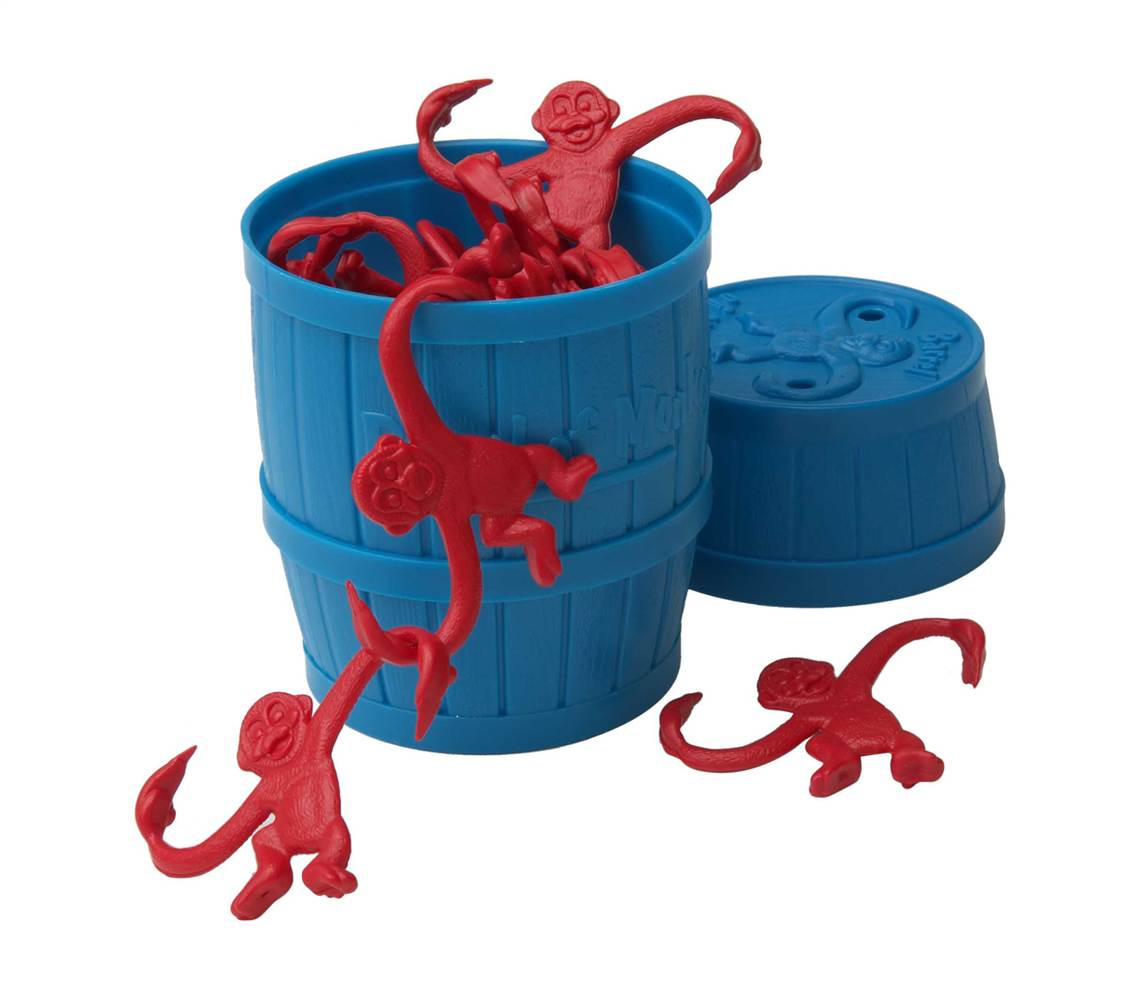
\includegraphics[width=12.1cm, height=9cm]{typescript/barrel-file/monkey-barrel}

\subsection{ Barrel File In Practice }
In the previous chapter we discussed doing something like the following:
\begin{lstlisting}
import {module} from '@ill/color-picker';
\end{lstlisting}

We are able to do this, because the nrwl nx layer on top Angular CLI, will
generate an index.tx file which will contain all imports. Anything that is
within the component, that should be exposed outside the lib, should be put
in the index.ts(barrel file).

\begin{lstlisting}[caption=index.ts]
export { IllColorPickerModule } from './src/ill-color-picker.module';
\end{lstlisting}

\subsection{ Enforcing Barrel File With Tslint }
In addition, Nrwl nx has a tslint add on called nx-enforce-module-bounderies.
\begin{lstlisting}
// tslint.json
"nx-enforce-module-boundaries": [
      true,
      {
        "allow": [],
        "depConstraints": [
          {
            "sourceTag": "*",
            "onlyDependOnLibsWithTags": [
              "*"
            ]
          }
        ]
      }
    ],
\end{lstlisting}

Adding true, will make the tslint complain whenever we are not using the barrel
import when accesing a lib file.


\section{ Typescript - Getting and Setting  }
Creating a getter and setter is a common occurance in OOP paradigm. When using
a class, Typescript offers an internal getter and setter. It is important to
note that within the Typescript documenation, a large part of the reason why
they create setters and getters, is to give a way of intercepting the setting
of a particular element. \footnote{typescriptlang.org\/docs\/handbook\/classes\.html}
For instance, let's say that you want to give people the ability for it to
error out if it doesn't actually contain one, or two strings. Doing something
like that with a setter is great.

\subsection{ Typescript - Why create a getter and setter? }
Another important point, is the syntactic sugar for two reasons.
\begin{enumerate}
  \item Getting and setting is a integral part of OOP programming. Before redux
  came around, it was literally a part of every component without a doubt.
  Having a functiin pegged with a get, or set directly before the function, helps
  specify the intent of the getter, or setter.
  \item While yes it is true, that one would be able to specifiy a function that
  will act as a setter or getter, it is syntactically, a bit awkward within an
  OOP setting. If I may:
  \begin{verbatim}
    getDinerText()
  \end{verbatim}

  \begin{verbatim}
    Diner.text
  \end{verbatim}
\end{enumerate}

So yes, can you set and get, without using the internal setter and getter that
Typescript has to offer like everything else, yes. However, the syntactic sugar
will make it seem like you are natively setting and getting. In addition,
putting emphasis on whenever an item is getted, or setted.

\subsection{ Valuable getting and setting within an ngrx/store setting }
So the question then becomes, if you are using ngrx/store within your app, for
what reason would you hvae value for getting and setting. For the most part, the
values that you have will either be set through @Input's within Angular, or
accessed through your @ngrx/store. There is one in particular very valuable
reason. That would be if within your Typescript component you have deep nested
data. Having a getter and setter within a component would be very useful. For
instance:
\begin{lstlisting}
get numberOfDocuments(): number {
  try {
    return this.userLog.user.documents.length;
  } catch (e) {
    return 0;
  }
}
\end{lstlisting}
Now we have a getter with logic, that says that if it doesn't exist, then it
will return something 0. We can then do something like the following:
\begin{verbatim}
<span> Number of Documents: {{ numberOfDocuments }} </span>
\end{verbatim}
in your html.

\maketitle{}
\section{ Typescript - Immutability }
Immutability is one of the core concepts when it comes to data. I first learnt
about it when I was introduced to Redux. However, as time progressed it was
something that I learn to integreate with all of my projects. With regards to
Typescript, it allows type annotations in the way of Immutability:
\begin{lstlisting}
export interface User {
  readonly firstName: string;
  readonly lastName: string;
}

let user: User = {
  firstName: 'Larry',
  lastName: 'Snow'
};

// This will result in a compile time error
person.firstName = 'Pam';

\end{lstlisting}

Instead this promotes using immutability. So if someone would like to turn this
data into something else, they would do something like the following:

\begin{lstlisting}
export interface NewUser extends User {
  location: string;
}
let newUser: NewUser = {
  ...user,
  location: 'New York'
};
\end{lstlisting}

\chapter{ Create a Custom Type Definition }
Typescript by default actually includes type definitions for all of core
Javascript. Any time you are using a core javascript method, typescript
within it's core framework has a typing for it. However, any time you
plan on using something not a part of core Typescript, you will have to
create a type definition. 

\section{Example Scenario}
For instance, in another chapter, we reccomend using the native Network 
Information API. Because it is experimental(atthe time of this writing),
as is the case in all scenarios, the Typescript team has not included 
type definitions for it. So, we need to go ahead, and create our own 
custom type definitions. 

In addition, there will be times within your Angular application, wherein 
due to the requirements of your organization, you might need to create your 
own custom type definition. Whether is be new technology, or simply security
concerns. 

The following is the cookie cutter process for creating a custom type 
definition within Typescript in Angular. 

\section{Create a Custom Type Definition File}
A custom type definition file, is a file that Typescript will automatically 
pull out. By default adding the type definition \lstinline{*.d.ts} suffix to
the app, will cause Typescript to know to use this type definition.

It is also important to note that as of Typescript 2.* and greater, the
tsconfig.json has two properties available: 
\begin{enumerate}
  \item \lstinline{typeRoots}
  \item \lstinline{types}
\end{enumerate}

\subsection{Type Roots}
Specifies the folder in which the Typescript transpiler should look for type 
definitions. This simplifies the process of being able to install npm packages.
Any typescript definition, can be created as an npm package underneath \lstinline{@types}.

\subsection{types}
Now that we have specified our \lstinline{typeRoots}, installed our type, into 
the \lstinline{@types} folder, all we need to do is specify it in our 
tsconfig.json file which types we want to use. Specifically within an Nrwl Nx 
setting, and it's mono-repo approach, there is a separate tsconfig.json file 
for every lib. That is where we will specify the types that we would like to 
use. 

\section{Example Code as is in Nrwl Workspace}
In the root \lstinline{tsconfig.json} file, the Angular CLI/Nrwl Nx has automatically
specify the root \lstinline{typeRoots} config for use, which is \lstinline{node_modules/@types}.
If we wanted, we could create our own package, and specify another 
\lstinline{typeRoots} to be used within Typescript. 
\begin{lstlisting}[caption=tsconfig.json]
{
  "compileOnSave": false,
  "compilerOptions": {
    "typeRoots": ["node_modules/@types"],
    "types": [],
    ...
  }
  "exclude": ["node_modules", "tmp"]
}
\end{lstlisting}

and then inside of our tsconfig.json file, Nrwl Nx will automatically generate
for us the types that we will be using within our lib. 
\begin{lstlisting}[caption=libs/common/services/tsconfig.json]
{
  "extends": "../../../tsconfig.json",
  "compilerOptions": {
    "types": ["node", "jest"]
  },
  "include": ["**/*.ts"]
} 
\end{lstlisting}

\section{Adding Our Own Custom Type NPM Package}
There are very few scenarios within Angular, wherein we would add our own 
custom types. I am of the opinion, that if you do find yourself having to 
add a custom type, let's make it available to everyone. I.e. let's open source 
our package, and make it something everyone can use. So let's run through the 
steps of creating our own NPM package. 

\subsection{Creating a Github Repo}
We have created a github repo entitled \lstinline{network-information-types}. 
We checked the box for initializing with a README, a .gitignore file for Node,
and a MIT license. We clone it locally by running: 
\begin{verbatim}
git clone git@github.com:razroo/network-information-types.git
\end{verbatim}

\subsection{Running npm init}
Next, we navigate to our newly cloned repo, and run: 
\begin{verbatim}
npm init -y
\end{verbatim}
The \lstinline{-y} tells the \lstinline{package.json} that we want to use all
default options. 
\begin{lstlisting}[caption=package.json]  
{
  "name": "project-name",
  "version": "0.0.1",
  "description": "Project Description",
  "main": "index.js",
  "scripts": {
    "test": "echo \"Error: no test specified\" && exit 1"
  },
  "repository": {
    "type": "git",
    "url": "the repositories url"
  },
  "author": "your name",
  "license": "N/A"
}
\end{lstlisting}

\subsection{Install Typescript and modify tsconfig.json}
First, let's go and install Typescript as a dev dependency: 
\begin{verbatim}
npm i typescript -D  
\end{verbatim}

Next, let's create a \lstinline{tsconfig.json} file and make it look like this:
\begin{lstlisting}
{
  "compilerOptions": {
    "target": "es5",
    "module": "commonjs",
    "declaration": true,
    "outDir": "./dist",
    "strict": true
  }
}  
\end{lstlisting}

\section{Adding a index.d.ts File}
When creating a custom type definition file, generally we will follow a three 
step process:
\begin{enumerate}
  \item Create Private Types
  \item Create Private Interfaces
  \item Create Public Interface 
  \item Extend Public Interface, to be Used/Consumed by Typescript
\end{enumerate}




\maketitle{}
\section{ Using Angular CLI in an Nx Workspace }

Now that we have created an nx workspace, let's create our app. Run
\begin{verbatim}
  ng g app angularPixelIllustrator --routing
\end{verbatim}

This will create an app called angular-pixel-illustrator\footnote{that's right
angular cli will automatically convert camel case to dash case} with routing
capabilities using the Angular CLI \footnote{If you will recall, we discussed
the Angular CLI folder/file directory in the Angular CLI Chapter}.

We can now serve\footnote{I.e. run on a server for development reasons} our app,
by running:
\begin{verbatim}
  ng serve
\end{verbatim} \footnote{It's important to note, that ng serve will open up
angularPixelIllustrator by default. As we begin to add more apps, it will make
more sense to specify specific app being opened.}


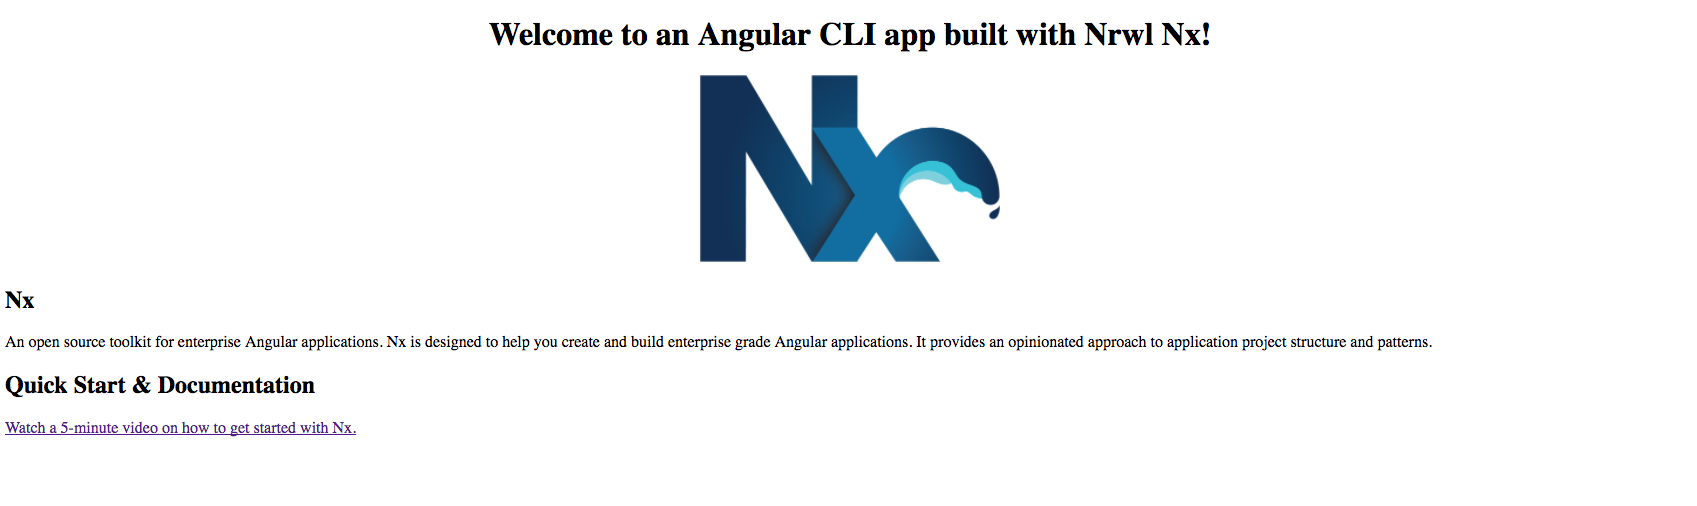
\includegraphics[width=13cm, height=9cm]{angular-cli-post-nx/angular_nx_initial_screen}

At this time, if you were to go to localhost:8080 you will see our app, is
ready to go.

Let's now create our first component. For our Pixel Illustrator, we want a form.
We will name the component chooseSize.

\subsection {Wait a Minute!}
Before we go ahead and create our component, we are going to want to tidy up
our folder architecture. The architecture we are introducing in this book is
heavily influenced by two projects. One, Nrwl, and by extension Nx. The other is
the example app, introduced in the ngrx/platform repo \footnote{It can be seen
here: https://github.com/ngrx/platform/tree/master/example-app}.

\subsubsection {Sidebar}
At the time of thiwriting there is one main area of conflict with regards to
ngrx/store v. Nx. Even though we have not experienced it yet, it makes sense to
talk about it before moving on from the cli/nx workspace chapters. Nx is very
opiniated with regards to it's folder structure. It believes everything should
be turned into it's own module, and all files related to that module should
be encapsulated inside of it. This includes (and if you are not familiar, do not
worry, we will get to it in later chaptes ) pipes, services, interfaces, guards,
and enums.

In the ngrx/example-app project, these will be split into separate folders, and
the appropriate file, will be put into that specific folder. I would imagine
that many on the ngrx/platform team agrees with nrwl/nx. I most certainly do,
and especially with state management, it makes sense for all others items to
be encapsulated into their appropiate folder. If it is something that should be
shared across app, then it should be put into it's own library. Something that
we will discuss moving forward.

\subsection {Phew, sidebar over, moving on}

The above being said, whenever we create a component, we are going to want to
encapsulate it, into a local module. That way we can add state, pipes, services,
you name it, and it will all be encapsulated in that component folder.

In order to create our module we run the following angular cli command:

\begin{verbatim}
  ng g module choose-size
\end{verbatim} \footnote{Once again we have the liberty with not having to
specify the app name}

Then, in order to create our component:
\begin{verbatim}
  ng g component choose-size
\end{verbatim}
The following five files have been created (using git diff --cached)
\begin{lstlisting}[breaklines]
new file:   apps/angular-pixel-illustrator/src/app/choose-size/choose-size.component.css
new file:   apps/angular-pixel-illustrator/src/app/choose-size/choose-size.component.html
new file:   apps/angular-pixel-illustrator/src/app/choose-size/choose-size.component.spec.ts
new file:   apps/angular-pixel-illustrator/src/app/choose-size/choose-size.component.ts
new file:   apps/angular-pixel-illustrator/src/app/choose-size/choose-size.module.ts
\end{lstlisting}


\section{ Format all the things }

In a Nrwl setting, we have a format npm script that is available to us by default.
It is called:

\begin{verbatim}
  nx format write
\end{verbatim}

This will call, a .prettier file that has been created by the nx workspace
command. Prettier is similar to to the CLI to the extent that there is a lot
that is happening behind the scenes. In short, it will automatically format files
for you, to it's liking. It's like a pro-active linter, that will format code
for you.

Two architectural talking points, with regards to prettier:
\begin{enumerate}
  \item You will have to format your tslint, so that it does not compete with prettier.
  \item You are going to want to hook up prettier with your IDE, so prettier
  can go to work without having to run it in your terminal.
\end{enumerate}

Note: We are going to have to create a way that we can update the prettier file
automatically.

\subsection{ How to add prettier to Webstorm }
As we mentioned in a previous chapter, Webstorm is our IDE of choice. VIM users
and Atom users, I completely respect your decision, and feel free to code in
that capacity. However, my experience working with large teams, is  that Webstorm
has a lot to offer outside of the box. For the non power user, it will offer
all of those benefits. Ok, great, the following is how to add prettier to Webstorm
with a screenshot!

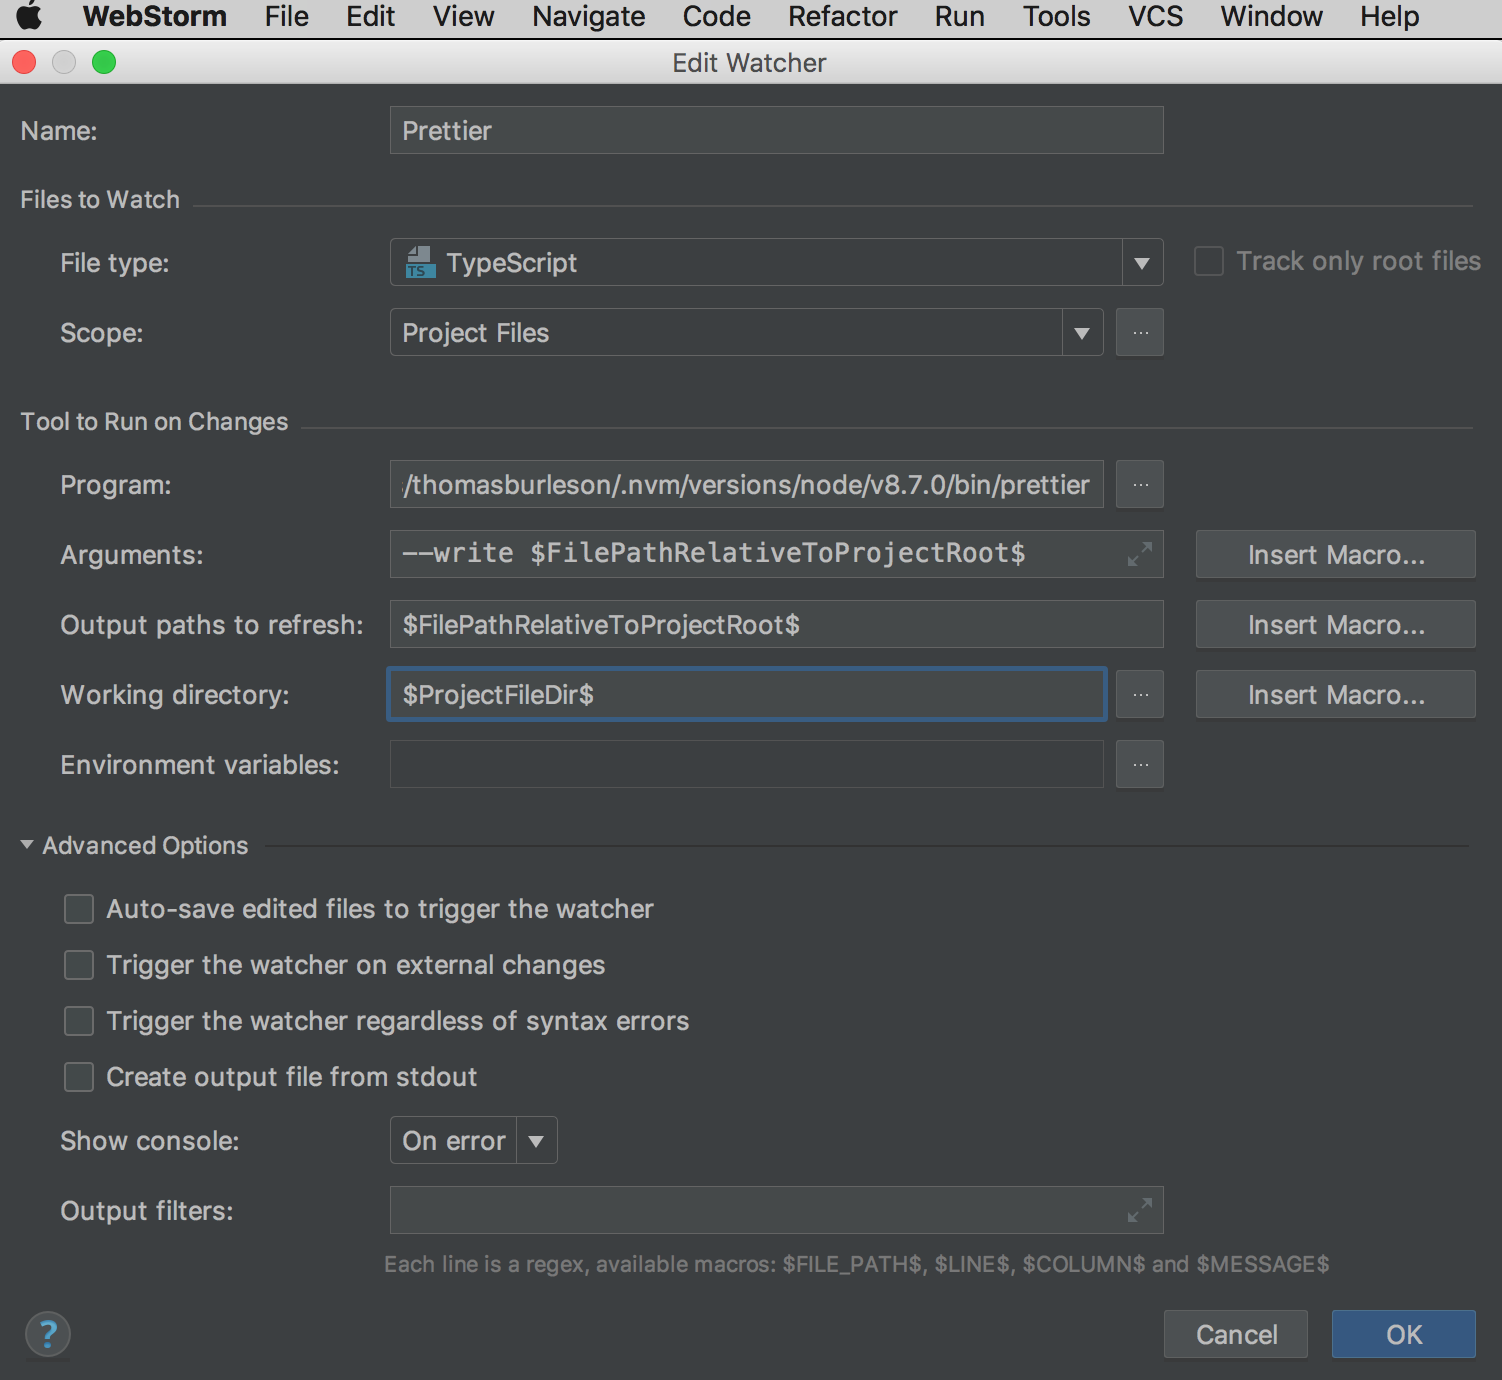
\includegraphics[scale=0.5]{format-all-the-things/prettier-file-watcher-webstorm}

\maketitle{}
\section{ Lint all the Things }

\subsection{ Lint all the Things }

Linting is incredibly important. Think of it this way. Someone's favorite food
item might be brocolli, another person's favorite food item, might be steak.
Now the two might work well together(on a number of levels, mmm hungry), but
forcing one person to adopt the other food item as their favorite, is unjust!

Ok, bad example, but the concept is the same. Things such as how many spaces per
indentation, double quotes vs. single quotes, trailing commas, empty interfaces,
these are all important points. To be honest, I've only found my peers arguing
on more minute points, such as double vs. single quotes, and how many spaces
per indentation. Therefore, linting allows:
\begin{enumerate}
  \item Agreement on code formatting rules.
  \item Automated way of keeping track of things that need to be changed.
  \item Self documentation through cli, on what needs to be changed.
\end{enumerate}

Another important point, is that we would ideally like a formatter, that
automatically formats these things for us. So, from an architectural perspective
when we are looking for a linter, we are also looking for a formatter to go along
with it.

\subsection{ What are we trying to lint? }
We are trying to lint HTML, SASS, and Typescipt. Angular CLI, offers Tslint out
of the box. 


\section{ Linting Sass }

As we mentioned in the previous chapter, there is a greate matter of importance
when it comes to linting. In particular when it comes to sass, the Angular CLI,
nor the Nrwl Nx cli will offer sass linting out of the box. In particular,
we will be choosing the package sass-lint.

\subsection{Installing Sass Lint}
\begin{verbatim}
  npm install sass-lint --save-dev
\end{verbatim}

\subsection{Adding a Lint Config File}
For sass-lint, it will hook into by default a file that is in the root of
folder called .sass-lint.yml. It's quite long, and you can see the rest of the
file in the actual github repo. However, you would create a sass-lint.yml file.
\begin{verbatim}
  touch sass-lint.yml
\end{verbatim}
Inside of the sass-lint.yml file, it will look something like this:
\begin{lstlisting}
options:
  formatter: stylish
files:
  include:
    - '{apps,libs}/**/*.scss'
  ignore:
    - 'libs/font-awesome/**/*.scss'
rules:
  # Extends
  extends-before-mixins: 1
  extends-before-declarations: 1
  placeholder-in-extend: 1

  # Mixins
  mixins-before-declarations: 1

  # Line Spacing
  one-declaration-per-line: 1
  empty-line-between-blocks: 1
  single-line-per-selector: 1

  # Disallows
  no-attribute-selectors: 0
  no-color-hex: 0
  no-color-keywords: 1
  no-color-literals: 1
  no-combinators: 0
  no-css-comments: 1
  no-debug: 1
\end{lstlisting}

The list for what sass-lint disallows goes on and on. Some of the linting rules
I really like is no color words, empty line between blocks, bem-depth, for
starters. From an architects perspective, and from a developers perspective, it
has made the code review process much easier. When this linting process is
combined with the functional sass paradigms we will mention, it becomes
self managing architecture for styling. Let me say that again, SELF MANAGING. I
thought that might be worth repeating.

\subsection{Adding an NPM Script in your package.json}
\begin{verbatim}
  "lint-scss": "sass-lint -v -q",
\end{verbatim}

\subsection{The Final Touch}

Adding the sass-lint npm script as part of your CI/CD architecture is what
really brings it all together. This is twofold of course. One so that when you
make a pr for your Github repo, it will check to make sure there are no Sass
linting errors. In addition, when pr is actually merged, pipeline runs as well,
to make sure there are no errors.

\maketitle{}
\section{ Linting HTML }

Linting html is not as mature as it is with regards to Sass and Javscript in my
opinion. Howvever, that makes sense as html is essentially strucutred xml that
is used within the context of a web app.

That being said, once again, there is no linter that is offered out of the box
through the Angular CLI, or Nrwl Nx either. It is, however, beneficial.

\mybox{
\subsection{ Side Bar }
Why not use something like Pug(once called Jade) for html templating. The main
benefit of something like Pug I have found is that it tells me where the html
begins and ends. In a complex html element, where there are many levels of
nesting this can be beneficial. However, in a templating engines, there tends to
be many quirks, in particular when it comes to using various frameworks. I have
rarely been on a team where after selling Pug, engineers have been enthusiastic
in using it.
}

\subsection{Why We Chose HTML Hint}
The honest truth is that the landscape for html hasn't drastically changed at
it's core level over the past couple of years. Of course, if there was a more
mature linter, the linter would complain that the engineer should use certain
html element as opposed to another. That being said, we have found html hint
to be the most robust html linter, even though development has been lack luster
over the past couple of years.

\subsection{Installing HTML Hint}
\begin{verbatim}
  npm install htmlhint --save-dev
\end{verbatim}

\subsection{Create an .htmlhintrc config file}
In the root of your app, create an .htmlhintrc file. The .htmlhintrc is set up
to be the default config name for html hint. A sample config for html hint will
just be a simple JSON object containing key values. For instance:
\begin{lstlisting}
{
  "attr-value-double-quotes": true,
  "src-not-empty": true,
  "alt-require": true,
}
\end{lstlisting}

\subsection{Adding an NPM Script in your package.json}
\begin{verbatim}
  "lint-html": "htmlhint --rulesdir './rules/' '{apps,libs}/**/*.html'",
\end{verbatim}

\subsection{Adding a Rules Directory for html hint}
You will notice that inside of our html hint command, we have created a rules
directory. We are doing this so that we can potentially create our own sample
html hint rule.

\subsection{What a Sample Rule Looks Like}
In the root of your directory, create a rules directory. Inside of that
directory, let's create some sample logic:
\begin{lstlisting}
module.exports = function(HTMLHint) {
  HTMLHint.addRule({
    id: 'attr-space',
    description: 'Attributes cannot have useless whitespace between "=" and attribute name or attribute value.',
    init: function(parser, reporter) {
      var self = this;

      function handleTagStart(event) {
        var col = event.col + event.tagName.length + 1;

        event.attrs
          .filter(function(attr) {
            return attr.value;
          })
          .forEach(function(attr) {
            var rawAttr = attr.raw;
            var indexOfEqualSign = rawAttr.indexOf('=');

            if (rawAttr.charAt(indexOfEqualSign - 1) === ' ') {
              reporter.warn('Space between attribute name and "="', event.line, col + attr.index + indexOfEqualSign - 1, self, attr.raw);
            }

            if (rawAttr.charAt(indexOfEqualSign + 1) === ' ') {
              reporter.warn('Space between "=" and attribute value', event.line, col + attr.index + indexOfEqualSign + 1, self, attr.raw);
            }
          });
      }

      parser.addListener('tagstart', handleTagStart);
    }
  });
};
\end{lstlisting}

The above allows for a robust html lint archticture, with the ability to add
more rules if need be.

\maketitle{}
\section{ Design Language System }

Creating a design language system is imperative to any architecture. Within
Angular the Full Gamut, we are going to assume that you are using Material
Design as your DLS. Reason as we discussed before, is that it is the most robust
library for creating Angular components. However, there are particulars of
Angular that one is going to want to modify. This is where having a light
design language system coming in can be very important.

\subsection{ Identifying Key Points of DLS }
The following are the 10 points that are a part of DLS:

\begin{enumerate}
  \item Colors
  \item Styles
  \item Icons
  \item Grid and Spacing
  \item Typography
  \item Buttons
  \item Form Controls
  \item Navigation
  \item Cards and Portlets
  \item Data Tables
\end{enumerate}

These are arguably the 10 parts of any material application that will be used
the most.

\subsection{ Identifying Proper Architecture }
With regards to overriding material design, is the part where architecture kicks
in. This is a very important part of the application and I will go through one
by one, the parts of the application that have similar architecture with regards
to overrides.

\subsubsection{ Colors }
Material design has the ability to be overriden in a sass file. It is important
to note, that the material theme allows for overrides using Sass Variables. So,
one would do something like this:
\begin{lstlisting}
@import 'src/styles/themes/blue-orange';
@import 'src/styles/material-overrides/material-overrides';
\end{lstlisting}

Doing something like the following:
\begin{lstlisting}
$gray-50: #fafafa;
$gray-200: #dbe1ea;
$gray-300: #e0e0e0;
$gray-400: #cccccc;
$gray-500: #bdbdbd;
$gray-600: #9b9b9b;
$gray-700: #757575;
$gray-800: #444444;
$gray-900: #212121;
\end{lstlisting}

Now the colors you have are specific to your app.

\subsubsection{ Grid and Spacing }
This one etc.

\maketitle{}
\section{ Material Design }

I was debating writing this chapter. The reason primarily being, that depending
on the size of your company, you might up end writing your own design system. I
completely understand that, and it makes sense if you are a B2C
\footnote{Business to Consumer} application, or a B2B application. If you are a
Business to Business application, then using an out of the box design system
probably makes sense. If you are building a cosumer application, I can see how
you would want your experience to be unique to that of other websites(granted
not working on an MVP).

However, I truly do not understand why a company using Angular, would not want
to use material design. It is the most robust design framework that exists
within open source. In addition, the documentation for Angular components is
next to none. I personally have been in companies where they had a business
to business applications and they decided not to use material design. It was an
absolute mess! I'll never forget the conversation we had 6 months in, wherein I
asked if it was possible for us to get design closer to the internal design
system we agreed on, so we can create the custom component! The designers
response is a classic! ``I thought the developers were doing that on their own!
''. Avoiding a scenario like this, is very difficult, and in my opinion, not
worth it for many team.

Companies choosing to use Material Design could have saved loads of resources
not having to design and implement their own components. It is out of the vast
amount of use cases that I see Material Design being valuable, that I have
decided to go ahead and write about it.

\subsection{ Material Design - Talking to UX/UI }
This section right here, is perhaps why I like Material Design the most.
Material Design has documentation for how the UX\footnote{User Experience}
should work. It also has an Angular Component Library with demos, that I can
show off to UX and show them, this is how it works by default. It addition,
theming for Material Design, is very easy.

\subsubsection{Theming your Material Design}
Putting your own company specific theme on it is generally very easy. In
addition, it can help alleviate any concerns those might have of using Angular
Material Components, due to it being possible to move over into a different
library. From professional experience, I have found the following to be the
cornerstone of what your team can expect to customize:
\begin{enumerate}
  \item Colors
  \item Font
  \item Spacing(Margin + Padding)
  \item Icons(not that this is anything particular)
  \item Buttons
\end{enumerate}

The above would be it for starters. As your designs go on, you will have
components that you will end up overriding. These will go in a partial sass
file, something that we will go into more detail as time goes on.

\subsection{ Material Design - Create your own Confluence Doc }
It is important when working with UX/UI to document discrepencies. For
inspiraiton look at the \href{https://material.io/guidelines/components/sliders.html}{material design docs}. The idea is to have a central place where UX can document the
differences they have made from the general Material DLS. Something like a
Confluence doc(if you are familiar with Atlassian), is a bit excessive. I have
found that it's too difficult for developers who spend the majority of their
time in code tools to document on confluence. In addition, for designers to
spend their time outside of the design tools(e.g. Sketch and Invision).

From a matter of ownership, engineering has a stronger discipline of
documentation and organization, due to code being very abstract at times.
Engineers should look to take ownership of the confluence doc. However, an
Invision doc, seems to be more efficient. Design should look to create an
Invision doc, that spans maybe 5 - 15 pages, on the DLS deviations they have
from actual Material Design.

\subsection{ Material Design - Use Invision }
It's interesting, because someone might not think of tooling as something which
is a part of engineering architecture. However, with regards to finding
discrepencies in DLS(Design Language System), Invision is integral. It will
make creating comments on particular components as something which will be fluid.

\subsection{ Material Design - Push Back }
The following will be worth alot of time for many different people within your
organization. Make sure that your component does not deviate from Material
Design. In addition, look into whether, or not it is pre-described for you to
go ahead, and create your own components. However, I can assure you designers,
product/business, and engineers will all be happy when you go with the default
components when possible. When building a product, unless it is beyond the MVP
go with what is available for you by default.

\subsection{ Material Design - Architecture Corner }
In a Material Design setting, there will be discrepencies in the design, which
we have mentioned above, two ways in order to address, and make sure that
engineering is in sync with Design.

However, how does Engineering make sure, that all engineers are adhering to the
principles layed out in the DLS. There are two methods which will help to a
great extent:
\begin{enumerate}
  \item Sass functions, with error reporting.
  \item Automating UI layer.
\end{enumerate}

\maketitle{}
\section{ Material Overrides }

Based on Razroo best practices, we have established the easiest way to get 
your app up and running, is to use material design within your Angular 
application. Generally, an organization will want to roll it's own theme into 
Angular Material. When that happens the developer will have to go ahead and 
customize the build for material design. Let's talk about how we can go ahead 
and do that. 

\subsection{Understanding Colors in Material}
First and foremost it is important to understand something called a color 
palette. I know some of you might be aware of what it is, but personally, I was
not aware. A color palette in the digital world, refers to the full range of 
colors that can be displayed on a device. Within a material design application 
it refers to the range of colors that can be used within the application. 
Material's design language makes use of two main colors for it's color palette: 

\subsubsection{Primary and Secondary Values}
\begin{enumerate}
  \item Primary - Color displayed most frequently across your app's screens and
  components. 
  \item Secondary - "Provides more ways to accent and distinguish your product."
  \begin{enumerate}
    \item Floating Action Button(Literally buttons that float over main content)
    \item Selection controls(sliders, switches etc.)
    \item Highlighting selected text
    \item Progress bars
    \item Links and headlines
  \end{enumerate}
\end{enumerate}

\subsubsection{Material Color Maps}

It will then create a series of light and dark variants based on the primary 
and secondary values. The primary and second values must be a map of colors 
going from lightest(50) to darkest(900). 

Material has already created a series of 16 color maps, for it's design system. 
An example of material green color map, for instance, will look something like 
this: 
\begin{lstlisting}
$mat-green: (
  50: #e8f5e9,
  100: #c8e6c9,
  200: #a5d6a7,
  300: #81c784,
  400: #66bb6a,
  500: #4caf50,
  600: #43a047,
  700: #388e3c,
  800: #2e7d32,
  900: #1b5e20,
  A100: #b9f6ca,
  A200: #69f0ae,
  A400: #00e676,
  A700: #00c853,
  contrast: (
    50: $dark-primary-text,
    100: $dark-primary-text,
    200: $dark-primary-text,
    300: $dark-primary-text,
    400: $dark-primary-text,
    500: $dark-primary-text,
    600: $light-primary-text,
    700: $light-primary-text,
    800: $light-primary-text,
    900: $light-primary-text,
    A100: $dark-primary-text,
    A200: $dark-primary-text,
    A400: $dark-primary-text,
    A700: $dark-primary-text,
  )
);
\end{lstlisting}

For primary values, the regular value will start at 500. For secondary values, 
the regular value will start at 200. The significagance of these values is that 
Material Design will follow a Hierarchical system. The darker the color is, the 
more of an emphasis we are placing on that button. The lighter it is, the less 
emphasis we are placing on that element. 

\mybox{You might be wondering about two things. For starters, why it is that 
the values progress by 100's. Second what is up with the values that have an 
"A" attached to the left side. Values progress by 100's is merely a convention
used by Material Desing. Other design frameworks progress by 10's(IBM Design)
instead of 100's, for instance, or even by 1's(Open Color). It is merely a
convention used to show that values are progressing.}

\subsection{Material Design and Sass}
First and foremost, we have already established that we will be working within
a Sass environment. Material Design offers Sass out of the box, and makes it 
incredibly easy to customize your environment based on sass overrrides. 

\subsection{Npm Install Material Theme}
First and foremost, let's make sure that we have properly installed and Angular
Material in our Angular application. 
\begin{lstlisting}
npm install --save @angular/material @angular/cdk @angular/animations
\end{lstlisting}

You package.json will now include packages needed to use Angular Material 
within the application in general. In addition, the package
(\lstinline{@angular/material}) to make the Sass changes we so dearly need. 

\subsection{Import Material Design and Call Core Styles}
The next step, is for us to go ahead and import Material Design in our 
\lstinline{styles.scss} file. The \lstinline{styles.scss} file can be found
in the root Angular application \lstinline{src} folder.

\begin{lstlisting}[caption=styles.scss]
@import '~@angular/material/theming';
// always include only once per project
@include mat-core();
\end{lstlisting}

\mybox{You will notice that we are adding a tilda\lstinline{\~} next to the
node module folder, containing the sass file we need. This tell the sass that
file we would like to import is located inside of the \lstinline{node\_modules}
folder.}

What the above does is import the \lstinline{theming.scss} file that contains
all of the theming variables for material design. We are also calling the
\lstinline{mat-core()} function, which is a, \begin{quote}
\say{Mixin that renders all of the core styles that are not theme-dependent.}
\end{quote} \footnote{This quote can be found in the \lstinline{_theming.scss}
file}

\subsection{Material Light + Dark Theme}
Angular offers out of the box in the \lstinline{_theming.scss} file a light and
dark theme function. The function looks a follows: 
\begin{lstlisting}
@function mat-light-theme($primary, $accent, $warn: mat-palette($mat-red)) {
  @return (
    primary: $primary,
    accent: $accent,
    warn: $warn,
    is-dark: false,
    foreground: $mat-light-theme-foreground,
    background: $mat-light-theme-background,
  );
}  
\end{lstlisting}

It takes in two required parameters: 
\begin{enumerate}
  \item primary - Primary color
  \item accent - Accent color 
\end{enumerate}
and one optional parameter called warn, which by default will be red. Material 
will also by default specify warn as being red. 

So let's say we wanted to create a custom theme based on some of the values 
that Angular provides, we can do the following: 

\begin{lstlisting}
$px-app-primary: mat-palette($mat-green);
$px-app-accent: mat-palette($mat-yellow);

$px-theme: mat-light-theme($px-app-primary, $px-app-accent);

@include angular-material-theme($px-theme);
\end{lstlisting}

Now all of our Angular Material components, will be using our unique theme.

\subsection{Creating Our Own Custom Theme}
Quite common your organization will want to layer their own custom theme 
outside of the 16 colors that Angular provides. This might manifest it's 
self in two scenarioes: 
\begin{enumerate}
  \item A new primary and secondary color
  \item In addition to new primary and secondary color, a new background and 
  foreground color as well. 
\end{enumerate}

Designers have a tool that allows them to automatically generate the appropriate
color in their design by supplying a singular color. Angular developers have
that luxury as well. There are tools that will do that for you. My personal 
favorite is the \href{http://mcg.mbitson.com}{Material Design Palette Generator}.
You will then have the ability to click on the clipboard icon, click on the 
dropdown for Angular JS 2 (Material 2), and copy the scss variable map. It's 
really as simple as that. 

\subsubsection{Create a \_themes.scss file}
Being that we are creating our own themes, the cleanest thing for us to do would 
be to place it in it's own \_themes.scss file. In addition, assuming that the 
organization is going to build out more applications, giving it the ability to
plug and play the companies theme, will really speed up development for other
parts of the company. That being said, Razroo best practices is to create a lib
folder for styles.

\begin{forest}
  [libs
    [common
      [styles
        [\_themes.scss,file]
      ]
    ]
  ]
\end{forest}

and inside of it, we are going to create a \lstinline{_themes.scss} file. Our 
generated themes using our primary, or seconday colors might look something 
like this:

\begin{lstlisting}
$razroo-primary-blue: (
  50 : #e7f2f4,
  100 : #c3dee4,
  200 : #9cc8d3,
  300 : #74b2c1,
  400 : #56a2b3,
  500 : #3891a6,
  600 : #32899e,
  700 : #2b7e95,
  800 : #24748b,
  900 : #17627b,
  A100 : #b3eaff,
  A200 : #80dcff,
  A400 : #4dcfff,
  A700 : #33c8ff,
  contrast: (
    50 : #000000,
    100 : #000000,
    200 : #000000,
    300 : #000000,
    400 : #000000,
    500 : #ffffff,
    600 : #ffffff,
    700 : #ffffff,
    800 : #ffffff,
    900 : #ffffff,
    A100 : #000000,
    A200 : #000000,
    A400 : #000000,
    A700 : #000000,
  )
);
\end{lstlisting}

It's quite a bit, but I just wanted to visualize that all of this is created by
using the Material Design Palette Generator. 

\subsection{Using Libs \_themes.scss file }
Inside of our \lstinline{styles.scss} file, we can import our 
\lstinline{\_themes.scss} file. Assuming we are just changing the primary color
and secondary color, we can do the following: 
\begin{lstlisting}
@import '~@angular/material/theming';
@import 'libs/common/styles/_themes';  

//@include angular-material-theme($mat-light-theme-background);
$razroo-theme: mat-light-theme(mat-palette($razroo-primary-blue), mat-palette($razroo-secondary-red));
@include angular-material-theme($razroo-theme);
\end{lstlisting}

We now have our own custom themes that we have created. They are available 
globally to be used by other applications/teams. In addition, using the Angular 
mat-light-theme funciton(mat-dark-theme also an option), or app is now using
our exclusive theme. 

\subsection{Background + Foreground}
It is important to mention that per the Material Design guidelines, background
and foreground are not meant to represent brand. They are more so used to 
convey the energy of the application. For Razroo's Pixel Illustrator, we wanted
to create a very vibrant appliation. This meant that we wanted to use our own 
background and foreground colors. Doing something like this requires a bit more 
of effort probably from the Material team expecting you to do it less. There 
are three steps required to change the background to what you want. 

\begin{enumerate}
  \item Generate color theme maps, using our Material Design Palette Generator
  \item Create a backround theme, and foreground theme for our application.
  \item Create our own custom theme function.
  \item Creating a default background for html + body, being that this will 
  only work as an override for material design components. 
\end{enumerate}

\begin{lstlisting}[caption=Example of what a custom background theme looks like.]
// Background palette for light themes.
$razroo-theme-background: (
  status-bar: map_get($razroo-background-yellow, 300),
  app-bar:    map_get($razroo-background-yellow, 100),
  background: map_get($razroo-background-yellow, 50),
  hover:      rgba(map_get($razroo-background-yellow, 500), 0.04), // TODO(kara): check style with Material Design UX
  card:       map_get($razroo-background-yellow, 500),
  dialog:     map_get($razroo-background-yellow, 500),
  disabled-button: rgba(map_get($razroo-background-yellow, 500), 0.12),
  raised-button: map_get($razroo-background-yellow, 500),
  focused-button: $dark-focused,
  selected-button: map_get($razroo-background-yellow, 300),
  selected-disabled-button: map_get($razroo-background-yellow, 400),
  disabled-button-toggle: map_get($razroo-background-yellow, 200),
  unselected-chip: map_get($razroo-background-yellow, 300),
  disabled-list-option: map_get($razroo-background-yellow, 200),
);
\end{lstlisting}

\mybox{Your team should have a designer who figures out what the opposite color 
of your background is, in order to create foreground. However, you can use a tool 
such as such as Color Tool's 
\href{https://www.colortools.net/color_complementary.html}{Opposite Color Tool}}.
Then you can follow up with the Material Design Color Palette tool, and
create the appropriate color map.

\begin{lstlisting}[caption=What custom theme function would look like]
@function razroo-theme($primary, $accent, $warn: mat-palette($mat-red)) {
  @return (
    primary: $primary,
    accent: $accent,
    warn: $warn,
    is-dark: false,
    foreground: $mat-light-theme-foreground,
    background: $razroo-theme-background,
  );
}  
\end{lstlisting}

\begin{lstlisting}[caption=html and body override]
//@include angular-material-theme($mat-light-theme-background);
$razroo-theme: razroo-theme(mat-palette($razroo-primary-blue), mat-palette($razroo-secondary-red));

// Include the default theme styles.
@include angular-material-theme($razroo-theme);  
\end{lstlisting}

\subsection{Overriding Components}
After we have overridden our theme in general across the app, there will be 
times wherein we will need to override specific styles for the component. 
There really isn't any way to modify the styling ahead of time. The only way
is to target the specific material component's class, and to modify it when 
appropriate. However, what we can do, is consolidate all of our overridden
 components in a singular place, so that it is well organized. For instance, 
 let's say that we have a dialog that we would like to remove padding for 
 in some scenarios, but keep it in others. We would put a dialog file inside of
 our material overrides folder. Our folder/file structure will look like the
 following: 

 \begin{forest}
  [libs
    [common
      [styles
        [material-overrides
          [\_dialog.scss,file]
          [\_material-overrides.scss,file]
        ]
        [\_themes.scss,file]
      ]
    ]
  ]
\end{forest}

\chapter{ Typography }

Typography at a design level, is a way of presenting text in an attractive 
fashion. In particular, this is at three levels: 
\begin{enumerate}
  \item Decipher different letters.
  \item Make blocks of elements, such as paragraphs, or headers, easy to 
  distinguish between each other. 
  \item Have text that draws you in, or speaks to you as a reader. 
\end{enumerate}

Typography in this regard is very unique. Because at it's core, it's 
not that complex. There maybe are 10-20 different elements to keep in
mind. However, because those 10-20 different elements get used literally 
everywhere, it makes typography the single most used item in your site. 

This book, as well as the creators (i.e. Razroo), are strong believers of 
using Material Design as part of your MVP. After that, moving onto some sort 
of other design language system as soon as your product is validated. So 
we reccomend the use of Material Design with Angular, and do indeed use it
throughout the book. Understanding how to override the typography, so that
you yourself can do it, and let your message, and brand bleed through the 
text is important. 

\section{Understanding Different Levels of Typography in Angular Material}
First and foremost, let's start at ground zero. Let's discuss the different 
levels of Angular Material Typography. The easiest way do this, is to copy 
and paste the sass function the material typography config. I have also 
added comments, to make it appropriate for the context of this book.

\begin{lstlisting}[caption=@angular/material/\_theming.scss]
// Represents a collection of typography levels.
// Defaults come from https://material.io/guidelines/style/typography.html
// Note: The spec doesn't mention letter spacing. The values here come from
// eyeballing it until it looked exactly like the spec examples.
@function mat-typography-config(
  $font-family:   'Roboto, "Helvetica Neue", sans-serif',
  // Large, one-off header, usually at the top of the page (e.g. a hero header).
  $display-4:     mat-typography-level(112px, 112px, 300, $letter-spacing: -0.05em),
  // Large, one-off header, usually at the top of the page (e.g. a hero header).
  $display-3:     mat-typography-level(56px, 56px, 400, $letter-spacing: -0.02em),
  // Large, one-off header, usually at the top of the page (e.g. a hero header).
  $display-2:     mat-typography-level(45px, 48px, 400, $letter-spacing: -0.005em),
  // Large, one-off header, usually at the top of the page (e.g. a hero header).
  $display-1:     mat-typography-level(34px, 40px, 400),
  // Section heading corresponding to the <h1> tag.
  $headline:      mat-typography-level(24px, 32px, 400),
  // Section heading corresponding to the <h2> tag.
  $title:         mat-typography-level(20px, 32px, 500),
  // Section heading corresponding to the <h3> tag.
  $subheading-2:  mat-typography-level(16px, 28px, 400),
  // Section heading corresponding to the <h4> tag.
  $subheading-1:  mat-typography-level(15px, 24px, 400),
  // Bolder body text.
  $body-2:        mat-typography-level(14px, 24px, 500),
  // Base body text.
  $body-1:        mat-typography-level(14px, 20px, 400),
  // Smaller body and hint text.
  $caption:       mat-typography-level(12px, 20px, 400),
  // Buttons and anchors.
  $button:        mat-typography-level(14px, 14px, 500),
  // Line-height must be unit-less fraction of the font-size.
  // Form input fields.
  $input:         mat-typography-level(inherit, 1.125, 400)
) {
  // ..rest of function goes here
}  
\end{lstlisting}

There are a total of 13 items, which we have the ability to override. Just an 
example, as to how these feed into general components throughout the site, and 
also in our actual app. Let's take two a look at two examples, to get an intuitive 
sense as to how we can implement Angular Material typography ourselves. 

\subsection{Angular Material Cards}
Let's dissect the Sass Mixin the Angular team uses for typography,
for the material card component. 
\begin{lstlisting}[caption=@angular/material/\_theming.scss]
@mixin mat-card-typography($config) {
  .mat-card {
    font-family: mat-font-family($config);
  }

  .mat-card-title {
    font: {
      size: mat-font-size($config, headline);
      weight: mat-font-weight($config, title);
    }
  }

  .mat-card-header .mat-card-title {
    font-size: mat-font-size($config, title);
  }

  .mat-card-subtitle,
  .mat-card-content {
    font-size: mat-font-size($config, body-1);
  }
}
\end{lstlisting}

\begin{enumerate}
  \item Title - Uses the config relating to h2 for size(\$headline), and 
  weight of equivalent for 
  \item Title within Header - Uses the config for title(h3) through and through.
  \item Subtitle and Content - Uses smaller body(\$body-1).
\end{enumerate}

This gives us a bit of an idea. The config, as expected, directly correlates to 
the purpose of the mat-card. It also brings home, that mat-card isn't meant to 
directly encompass content of a page, and rather for minor pieces of content 
here and there. 

\subsection{Angular Material Headers}
It is important to note, that the Angular Material theme will not by default 
change native elements. HTML Elements such as headers(\lstinline{<h1>, <h2>, <h3>}), 
list items(\lstinline{<li>}), and \lstinline{<p>} tagswill have not have default 
material styling. However, material design does have it's own internal typography 
system, that can be seen here: 
\begin{lstlisting}[caption=@angular/material/\_theming.scss]
@mixin mat-base-typography($config, $selector: '.mat-typography') {
  .mat-h1, .mat-headline, #{$selector} h1 {
    @include mat-typography-level-to-styles($config, headline);
    margin: 0 0 16px;
  }

  .mat-h2, .mat-title, #{$selector} h2 {
    @include mat-typography-level-to-styles($config, title);
    margin: 0 0 16px;
  }

  .mat-h3, .mat-subheading-2, #{$selector} h3 {
    @include mat-typography-level-to-styles($config, subheading-2);
    margin: 0 0 16px;
  }

  .mat-h4, .mat-subheading-1, #{$selector} h4 {
    @include mat-typography-level-to-styles($config, subheading-1);
    margin: 0 0 16px;
  }  
  // ...
}
\end{lstlisting}

In the above, we can see that Angular Material stays true to the Material
spec, and applies the respective style. I.e. 
\begin{enumerate}
  \item .mat-h1 - headline
  \item .mat-h2 - title
  \item .mat-h3 - subheading-2
  \item .mat-h4 - subheading-1
\end{enumerate}


\chapter{ UI Skeleton }

Real data, very rarely, will be immediately available. 

Even if your app has a very quick backend service, due to other web applications the user might be using,  bandwidth can affect the time it takes to load. 

It can be a very uncomfortable experience for the user if they are unaware of what is happening. That's why loaders are important.

Within a design language system, a UI Skeleton, or Ghost Elements, as it should probably be called, is a good idea. 

It often comes in the form of gray boxes marking out the UI components awaiting action. It gives the user a rough indication that something is coming soon. It is a very simple way of easing anxiety of the user, and allowing them to be aware of all times, that something is loading.

\section{ One True Way of Implementing Ghost Views }
There are three options of implementing Ghost Elements.
\begin{enumerate}
  \item Creating an Overlay Ghost Element
  \item Creating an Inline Ghost Element
  \item Inline Ghosts with Async Loads
\end{enumerate}

\section{Why not to use an Overlay Ghost Element}
I would personally not recommend using an Overlay Ghost Element. It requires that developers determine when Ghost it removed. In addition, it requires for layouts to match the ``Real'' DOM layouts. However, DOM layouts are changing all the time, and this solution is not a good long term solution. Most definitely not an enterprise solution.

\section{ Why not to use an Inline Ghost Element }
There is an option to have a css only option. That is, that the css class changes based on whether, or not the data is available. The only real issue with this solution, is that it will be more of an off/on switch with regards to transitioning between a ghost element and an inline element.

\section{ Why use Inline Ghosts with Async Loads}
This is a very sophisticated solution, which I first saw from a one Thomas Burleson. The idea, is that we create a queryState function:
\begin{lstlisting}
/**
 * Wrapper function to easily determine async state
 */
export function queryState<T>(item:AsyncItem<T>) {
  return {
    isPolling : (item.state === AsyncItemState.POLLING),
    isLoading : (item.state === AsyncItemState.LOADING),
    isLoaded  : (item.state === AsyncItemState.LOADED)
  };
}
\end{lstlisting}

Then, inside of our component, we can go ahead and call the queryState within our component.

\begin{lstlisting}
export class UserListComponent {
  state = queryState;
  user$ = this.facade.users$;
}
\end{lstlisting}

Here, we can create numerous states including polling. This is a more robust solution than using plain css.

\section{ Ghost Elements Always? }
There are scenarios wherein a ghost element might not be the ideal scenario.

\section{Key Take Aways}
\begin{enumerate}
  \item Angular Animations can be implemented as re-usable recipes.
  \item AsyncItem is a general pattern used to decorate server entity items with
  `client side data state'
  \item Each Ghost component is a custom component crafted for that specific
  component. The odds of it being re-usable is next to none.
  \item Ghost grades and annimations are re-usable.
\end{enumerate}

Ghosts might simply be css.


\chapter{ Icons }

I would like to dedicate a quick chapter to icons, simply because I have never
come across an application that has not used icons. In addition, every app has
to make the decision, what icons they are going to use. It's interesting,
because I had less of a hesitation to write this chapter, than I did for
Material Design. With regards to icons, the choice is really ubiqitious at this
point. If you are going to use icons, it should be Font Awesome!

\section{ Font Awesome }
In short, font-awesome is the largest icon library currently available, and the
pro version is relatively cheap. In addition, there are many particulars with
icons that they solve, making sure that they look good on different devices. So,
in short I would like to reccomend font-awesome. It is the best architectural
decision you can make when it comes to fonts. Of course, unless your team has
the need to use their own icons. However, before proceeding to do so, let's
discuss some of the benefits of using Font Awesome:
\begin{enumerate}
  \item Pixel Perfect, Consistent Look.
  \item 5,000 icons and growing.
  \item Ability to play with Size on Web.
  \item Accesibility Minded
  \item Desktop Friendly.
  \item Tried and Tested, by the whole community.
  \item Multiple ways to use. CDN, Download yourself, install via NPM.
\end{enumerate}

Font Awesome truly is ubiqitious on the web. In the past 10 years that I have
been using it, it is the only consistent tool that has been used across
companies.


\section{ Sass Error Reporting }

I have decided to include the chapter on Sass Error Reporting in the chapter
for Design Language System. The main reason for this, is that any core style is
going to be considered as part of the core Design Language System. However, it
can be very difficult to maintain a core design, without some safe guards in
place, to make sure it is consistent across the app.

\subsection{ When to use Sass Error Reporting }
One should use Sass Error reporting if it is a core style. It is a core style if
it is used in more than one page, as a foundational piece of styling, non
unique to specific component.

\subsection{ What We Are Looking For With Using Sass Functions }
\begin{enumerate}
  \item No values other than these are used
  \item When a Pr comes our way, and we say to use the above, we have a function which is self documenting.
  \item Have a UI of sorts that also trains developers on how the internal of
  the DLS works, so that they should be aware if anything is wrong.
\end{enumerate}

The following is a great example of what a core design function would look like.
\begin{lstlisting}
// Gutter variables, for padding + margin
// function to take in multiplier(8), which must emit of one of values within ill-space-amounts
@function ill-space-multiplier($n) {
  $ill-space-amounts: (0, 4, 8, 16, 24, 32, 40, 48, 56, 64);
  $ill-space-multiplier: 8;

  @if(index($ill-space-amounts, ($n * $ill-space-multiplier))) {
    @return #{$n * $ill-space-multiplier}px;
  }
  @else {
    @error "Must contain one of the following numbers: #{$ill-space-amounts}.";
  }
}
\end{lstlisting}

If we have any component that is going to go ahead and use this function, we
can simply go ahead and use it:

\begin{lstlisting}
@import 'src/styles/variables';

:host {
  padding: ill-space-multiplier(2);
}
\end{lstlisting}

In this particular situation this helps, so that if the input passed to the
multiplier is not a number, it will complain. In addition, if the result is not
one of the multipliers, it will complain as well. So for instance, if the number
passed in, is 1.5, it will cause the function to error out, being that there is
no number 12, that is one of the ill space amounts.

\subsection{ Applying Architecture to Design Language System as a whole? }
The truth is that this pattern only applicable to padding, and spacing. For
instance, we technically could create a function for breakpoints:
\begin{lstlisting}
// breakpoints to be used in conjunction with media queries across app
@function ill-breakpoint($breakpoint) {
  $breakpoints: (
    'small': 400,
    'medium': 720,
    'large': 1024,
    'extra-large': 1424
  );
  @if (map-get($breakpoints, $breakpoint)) {
    @return #{map-get($breakpoints, $breakpoint)}px;
  } @else {
    @error 'Must contain one of the following strings: #{$breakpoints}.';
  }
}
\end{lstlisting}

However, we reccomend the use of flex-layout. Flex layout currently does not
have the ability to use this pattern. Nonetheless, for padding, and spacing
alone, this singular piece of sass functionality will probably be used on a
daily basis, and is very much so worth it. 

\maketitle{}
\section{ Creating Code Owners }

As we have discussed previously, Github is our preferred client for pull
requests. As the team grows larger it becomes imperative, that default code
reviewers are setup. Creating a \codeowners{} file is the easiest way to do this.

\section{ What is a \codeowners{} file? }
A \codeowners{} file is a config file, used with Github, that will allow you to
specify which github users are considered as \codeowners{} for a specific project.
In addition, it will allow you to target \codeowners{} for a specific file type.
So just to go a bit more in detail, let's say you have a dynamic team, and a
dynamic codebase. Part of the team develops in Python, and part of the team
develops in Javascript. You would be able to set \codeowners{} specifically for
javascript, so that if only js files have been affected, only these specific
\codeowners{} should be brought up.

\section{ How to create a \codeowners{} file? }
There are two places wherein you can create a \codeowners{} file. One would be
in the root of your app. The other would be in a .github folder in the root of
your repo. We recommend the .github folder, as we will also be creating webhooks
within our repo. So:
\begin{verbatim}
  mkdir .github; cd .github; touch \codeowners{}
\end{verbatim}
When you make a pull request within your github app, github will automatically
pick up on this file.

\maketitle{}
\section{ Code Reviews }
Code reviews are a very intuitive process. It can potentially be looked at as
something that I would do. If the pull request isn't looking at the code the
same way I would, then I should comment. However, it's the part of commenting
and accepting criticism, that makes this is entire process very tricky.

\subsection{ Code Reviews - The Golden Rule }
There are multiple ways of doing something. If the code reviewer leaves a
comment for doing something in an alternate way, and the person recieving the
code resists, then the code reviewer has no right to insist on her/his way. It
is then important, however, from that point onwards, that the team agrees on a
convention.

\mybox{\subsection{Story Time}
  The following is a great example of how this golden rule can manifest in real
  life. Once upon a time, my team was working on a component, wherein every tab
  was to be in uppercase. The person submitting the code felt that explicitly
  typing out every word in uppercase: NAME, STATUS, TIME; Made more sense. I
  expressed that adding a css class with text-transform: uppercase;
  would make more sense. The pr submitter expressed that they felt explicitly
  typing out everything made more sense. I mentioned that ok, I can see your
  point of view, and I will remove my comment.

  The truth is that if this was a B2C\footnote{Business to Consumer}
  application, then I would have been adament about my approach. However, this
  was a B2B\footnote{Business to Business} application, and allowing this person
  to code the way they feel comfortable and be happy, because life really is too
  short, is ultimately what is important.
}

\subsection{Setting Conventions}
Another important part of the code review process is to set conventions. In my
humble opinion, the reason conflict happens with regards to code, is due to
uncertainty. When there are conventions set up before work on code happens it is
to point to code guidelines and say this is what we do. In addition, somone has
the ability to challenge code guidelines, and it is more challenging code
guidelines. This allows those involved in discussion to save face.

\subsection{ A Time to Learn }
It is also very important for others to learn. It is a way for me as the code
reviewer to ask what a certain piece of code does. A good convention is that if
it is something new that you haven't done before, then you can ask about it
and learn about it. This is one of those points that is obvious yet it is passed
on more than most.

\subsection{ A Time to Mentor }
It is also a time to setup \codeowners{} across the app, and specifically make
junior developers code owners. 

\maketitle{}
\section{ Github Wiki }


\section{ Github Board }

The github board, for open source projects is used in a task management
capacity. In an enterprise setting, it can be used to track the one thing
that can't be tracked through JIRA, app considerations.

For instance, let's say you would like to migrate your app to the latest version
of Angular. You would create a board called "Tech Concerns". You would then go
ahead and create a widget for Upgrade Angular. Everyone on your team would then
know that you have certain things that you would like to progress in tech.
This can be used for other items as well, such as change directory structure to
use mono repo, or integrate E2E tests within app.

\maketitle{}
\section{ Smart Vs Dumb Components }

In any UI framework

\maketitle{}
\section{ Dialogs }

There are certain components that are expected in any architecture. Dialogs are
one of those components. However, their architecture can be so complex, that it
is very important to come up with a strategy that works with state management.
This architecture was originally adopted from Thomas Burleson who I have a
tremendous amount of respect for.

A couple of issues that dialogs have, is that they are:
\begin{enumerate}
  \item Defined in Templates
  \item Created at App Startup
  \item Managed in UI Components
  \item They complicate UI Components
    \begin{enumerate}
      \item Open, close, cancel
      \item Services
      \item Store Actions
      \item Pending State
    \end{enumerate}
  \item Dialogs may interupt NgRx Flows
\end{enumerate}

\subsection{ Centralizing Dialogs + Best Practices}
As with the rest of our architecture, we are trying to centralize the way we
use our components. Therefore, the following are dialogs best practices:
Section 1
\begin{enumerate}
  \item Use @angular/material Dialogs
  \item Use Dialog Service to open and and manage custom dialog components
  \item Use Dialog configurations to customize dialog instance
\end{enumerate}
\begin{enumerate}
  \item Use Ngrx Effects to Manage Dialogs
  \item Inject Store/Facade into Dialog Components
\end{enumerate}

\begin{enumerate}
  \item Use Ngrx Dialog Effects
  \item Disconnect Dialog from Feature Effects
\end{enumerate}

\maketitle{}
\section{ Dependency Graph }

A dependency graph is a very simple way of seeing which components are
dependent on which components. It goes hand in hand with a parent and child
component architecture.

\maketitle{}
\section{ Containers, Routing + Ngrx/router }

We now have a choose-size component, as well as a choose-size module.
The dynamics of our app, is that there will only be two parent pages. One will
be the choose-size page. The other will be the draw page. When a user goes to
the page for the first time, they will see the choose-size page. Therefore we
are going to add two routes in our app.

In our app.module.ts, we will use the existing RouterModule that has been
created by Nx, and include it in our RouterModule:

\begin{verbatim}
  // Inside imports add
   RouterModule.forRoot([
    {
      path: '',
      redirectTo: 'choose-size',
      pathMatch: 'full'
    },
    {
      path: 'choose-size',
      component: ChooseSizeComponent
    }
\end{verbatim}

\marginpar{git commit -m 'Add a routes to the RouterModule, for the choose-size page.'}

Now that we have redirected the default homepage to re-direct to the
choose-size page, let's try it out. Open up http://localhost:4200, and your page
should navigate to the choose-size page, with the text, "Choose Size Works",
towards the bottom of the page.

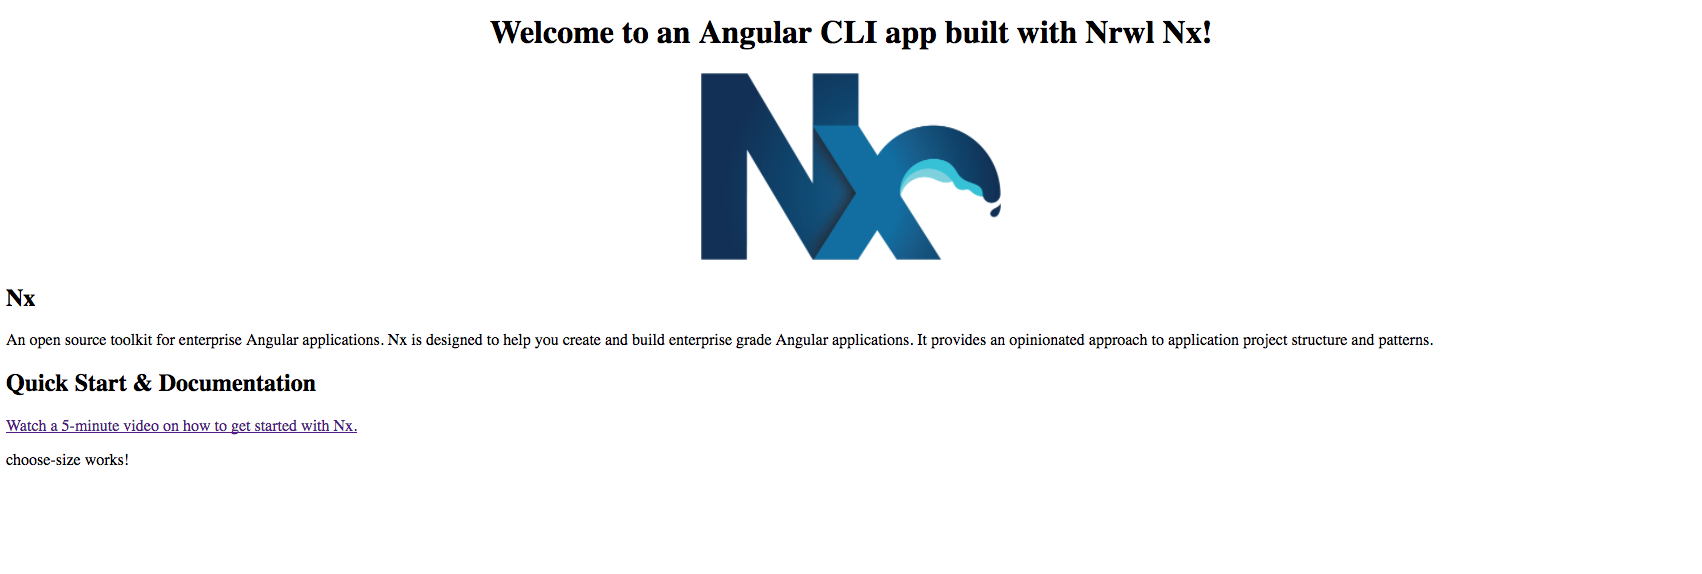
\includegraphics[width=13cm, height=9cm]{routing/containers-and-routing/choose-size-screenshot}

\subsection{ ngrx/router-store }

Before we move any further with regards to angular routes, let's discuss
ngrx/router. In short, ngrx/router exists so that the route can be in the store
as well. By default ngrx/router will dispatch a ROUTER\_NAVIGATION action
\footnote{We'll discuss this a bit more when we get to the chapter on ngrx/store},
when a navigation route get's called. This will enable time traveling with
regards to routes.

\subsection{ Why use ngrx/router-store }

Ngrx/router-store can be advantageous in two regards. One, it adheres to the
principle of there being a single state of truth \footnote{https://redux.js.org/docs/introduction/ThreePrinciples.html\#single-source-of-truth}.
Two, it helps applications with regards to breadcrumbs, and adding filters to the
url. If one wanted to follow an architecture, where the route contains the current
state of the application(filters, inputs etc.) router-store definitely make's it
very easy to do so.

\subsection{ Adding ngrx/router-store to our app }

In order to add ngrx/router-store to our app, run:
\begin{verbatim}
  npm install @ngrx/router-store --save
\end{verbatim}

In addition, we will be adding the route to our store for the first time, so we
will be needing ngrx/store. Please run \footnote{This will also install ngrx/store-devtools + ngrx/effects}:
\begin{verbatim}
  npm install @ngrx/store --save
\end{verbatim}

In our app.module.ts we will be adding the following:
\begin{lstlisting}[caption=My Javascript Example]
  + import { StoreModule } from '@ngrx/store';
  + import { StoreRouterConnectingModule, routerReducer } from '@ngrx/router-store';
  + import { StoreDevtoolsModule } from '@ngrx/store-devtools';
  // inside of imports
  + StoreModule.forRoot({
  +    router: routerReducer
  + }),
  + StoreRouterConnectingModule.forRoot({
  +   stateKey: 'router'
  + });
  + StoreDevtoolsModule.instrument({
  +    maxAge: 5
  + }),
\end{lstlisting}

\subsubsection{ Side note when using devtools with ngrx/router-store }

One final note when using ngrx/store router-store with devtools. The
RouteStateSnapshot is a very large object, containing large amounts of data. I've
run across performance issues, it is therefore reccomend setting up a
custom router state serializer
\footnote{https://github.com/ngrx/platform/blob/master/docs/router-store/api.md\#custom-router-state-serializer}.
The idea is that the user provides the specific items one wants from the route.
This allows for maybe 3 key/values to appear, instead of a 1000+. For the sake of
brevity, we will not include the technical steps here. However, the code for doing
so can be found in the github branch equivalent.

Now that we have our first route set up, as well as ngrx/router-store, let's proceed
to building a component.


\chapter{ Lazy Loading Modules }
Lazy loading is one of the many overlooked pieces of UI Architecture. The idea of lazy loadin is loading
something as it is required rather than all at once on page load. It's a form of page 'procrastination' if you think of it that way - only do things at the very last moment and as required. When it comes to Angular, lazy loading is part of the routing/module architecture and is heavily tied to routing. 

The main benefit of lazy loading is that on initial load of the web page we drastically decrease the bundle size. This improves user experience. Thankfully, Angular  makes it relatively easy to include a lazy loaded module into the app. 

The Angular CLI even has a command, for easily setting up a lazy loaded route. However, before we go ahead and show the command, that automatically scaffolds lazy loading for us, let's discuss how to add a lazy loaded route if we were to do that process manually. 

\section{Adding a Lazy Loaded Module Using Angular CLI}
\begin{verbatim}
  ng g lib about --routing --lazy --directory=razroo
\end{verbatim}

This command will automatically add a module to our lib. In addition, will modify the route within the about.module.ts, so that it can be used as a lazy loaded route. 

\mybox{An important note is that all the additional --routing --lazy flags will
add is this line: 
RouterModule.forChild([
  /* {path: '', pathMatch: 'full', component: InsertYourComponentHere} */
])

If you are upgrading an existing module to use lazy loading, the following directions will work for you as well. 
}

\section{What We Should Edit Post Generation}
Now that we have generated a route for our "about" page, let's make the two edits required post CLI generation. 

\subsection{Editing app.module.routing.ts File}
Edit one, will be in our main \lstinline{app.module.routing.ts} file:
\begin{lstlisting}
{
  path: 'about',
  loadChildren: () =>  
    import('@razroo/razroo/about').then(
      module => module.RazrooAboutModule
    )
},
\end{lstlisting}
\footnote{Just in case you are familiar with a different syntax, this is the latest syntax for Angular 8+.}

You will notice two things in the above code: 
\begin{enumerate}
  \item A \lstinline{path} key, standard for Angular routing, to specify what 
  module should be loaded when navigating to a specific route. 
  \item A \lstinline{loadChildren} key, which calls a function followed by the 
  standard syntax for importing a module. 
\end{enumerate}

In addition, being that we are using Nrwl Nx (which this book is littered with)
the import path is using our Nx workspaces shortened path. Here that would be the 
\lstinline{razroo-workspace/razroo-lib/lib-name}.

The second edit for us to make, will be in the actual module for our about page: 
\begin{lstlisting}
@NgModule({
  imports: [
    //...
    RouterModule.forChild([
      {path: '', pathMatch: 'full', component: AboutComponent}
    ])
  ],
  declarations: [AboutComponent]
})
export class RazrooAboutModule {}
\end{lstlisting}

\mybox{You will notice that in the above code we are actually using an AboutComponent. This component will need to be generated in addition to module we've already created, and can be done simply by navigating to our libs folder, and runnning \lstinline{ng g component about}.
}

The above is the cookie cutter process involved with creating a lazy loaded module within an Angular application. With Angular, it is relatively painless process for what it is accomplishing. It is architecture that is worth implementing early on in the app. It might save you from circular dependency nightmares later on. 
\chapter{ Lazy Loading Images }

Even though we discussed lazy loading modules, we might also want to lazy load 
the content inside of the lazily loaded modules. There is a very popular 
article from \href{https://www.thinkwithgoogle.com/marketing-resources/data-measurement/mobile-page-speed-new-industry-benchmarks/}{Google} 
that is generally spread around with regards to performance for webpages. 
In short, it presents the following very persuasive set of data: 

\begin{center}
  \begin{tabular}{@{} l *4c @{}}
    \toprule
    {\color{red}As page load time increases}\\
    \toprule
    {\color{red}Seconds} & Probability of Bounce \\
    \midrule
    1s to 3s       & Increases by 32\% \\
    1s to 5s       & Increases by 90\% \\
    1s to 6s       & Increases by 106\% \\
    1s to 10s       & Increases by 123\% \\
  \end{tabular}
\end{center}  

As we can see with the data presented above, performance of our webpages are 
very important. More so it presents the data very clearly that the faster 
a webpage is, the higher probability there is to retain our user base. 

\section{The Idea of Lazy Loading Images}
There are, of course, many different ways to increase performance. The intent 
of this chapter, however, is just to discuss the one performance boost that 
is gained by lazy loading images. The idea of lazy loading images, similar 
to lazy loading modules in general, is to load an image only when a user 
get's to that image. 

\subsection{Side bar - User Experience and Lazy Loaded Images}
It is important to note, that we do not want to lazy load all images
that are present on our page. For instance, imagine that we were creating a 
blog for our website. On each single blog page, we have a feature image 
that shows up first for our blog. In addition, we have more images that 
show up throughout the remainder of the blog. It can be strongly argued 
that lazy loading should not be applied to the feature image. Because, it 
would potentially cause an awkward experience for the user, to load the page 
and then wait an additional second to see what the feature image looks like. 

Therefore, when creating lazy loaded images, it is important to not create a 
blanket rule that will apply to all images. Rather, those images which are not 
primary to the page, those should be lazy loaded. 

\section{ Real Talk - Implementing Lazy Loading }
Within Angular, there would be a way to implement lazy loading from scratch. 
The simplest solution I've seen is wrapping an Angular Directive around the 
\lstinline{Intersection Observer} api. It will allow you to determine when 
an element is in the viewport. 
This \href{https://blog.angularindepth.com/a-modern-solution-to-lazy-loading-using-intersection-observer-9280c149bbc}{approach}
, works great, however, there are readily available npm plugins that do this for Angular. 
While the author of the aforementioned article did create their own \href{https://github.com/TradeMe/ng-defer-load}{plugin}
there is another that is much more mature. It implements the intersection 
observer as well, and is called \lstinline{ng-lazyload-image}.

\section{ng-lazyload-images}
Razroo's preferred package is ng-lazyload-image. It is the most mature of 
all packages in the Angular eco-system, has the most stars, and fantastic 
documentation. 

\subsection{Install}
\begin{lstlisting}[language=bash]
npm install ng-lazyload-image --save
\end{lstlisting}

\subsection{Setup}
\begin{lstlisting}[language=javascript]
import { NgModule } from '@angular/core';
import { BrowserModule } from '@angular/platform-browser';
import { LazyLoadImageModule } from 'ng-lazyload-image'; // <-- import it
import { AppComponent } from './app.component';

@NgModule({
    declarations: [ AppComponent ],
    imports: [ BrowserModule, LazyLoadImageModule ], // <-- and include it
    bootstrap: [ AppComponent ]
})
export class MyAppModule {}
\end{lstlisting}

\mybox{
\subsection{If Using IE}
If want to use IE, will need to use a polyfill. 
}

\begin{lstlisting}[language=javascript]
  import { NgModule } from '@angular/core';
  import { BrowserModule } from '@angular/platform-browser';
  import { LazyLoadImageModule, intersectionObserverPreset } from 'ng-lazyload-image'; // <-- include intersectionObserverPreset
  import { AppComponent } from './app.component';
  
  @NgModule({
      declarations: [ AppComponent ],
      imports: [
        BrowserModule,
        LazyLoadImageModule.forRoot({
          preset: intersectionObserverPreset // <-- tell LazyLoadImage that you want to use IntersectionObserver
        })
      ],
      bootstrap: [ AppComponent ]
  })
  export class MyAppModule {}
\end{lstlisting}

\section{Example Use Case}
The following is an example use case, of how to create a lazy loaded image 
with ng-lazy-load: 
\begin{lstlisting}[language=javascript]
import { Component } from '@angular/core';

@Component({
  selector: 'image',
  template: `
    <img [defaultImage]="defaultImage" [lazyLoad]="image">
  `
})
class ImageComponent {
  defaultImage = 'https://www.placecage.com/1000/1000';
  image = 'https://images.unsplash.com/photo-1443890923422-7819ed4101c0?fm=jpg';
}
\end{lstlisting}

The package also has examples for multiple other use cases such as background 
images, responsive images, async images(i.e. \lstinline{| async}) etc. 

\section{Transitioning Photos}
Something that you might want to do is add a transition to your photo, so that 
it swaps out the defaultImage with the lazyLoaded image. Doing something like 
this would be relatively straightforward. For instance: 
\begin{lstlisting}
img.ng-lazyloaded {
  animation: fadein .5s;
}
@keyframes fadein {
  from { opacity: 0; }
  to   { opacity: 1; }
}  
\end{lstlisting}

That is all it would take to put a transition effect on your photos.

\section{ Hooking Up Lazy Loading To Our Back End }
I am going to assume that the reader is intelligent enough to figure out how to
hook up the backend to their component, without the need of this book. Therefore, 
I just wanted to mention the strategy really quick. In short, you would get all 
image urls from the actual GraphQL query. You would put them underneath the 
\lstinline{lazyload} directive. Just like that you have lazy loaded configured. 


\chapter{ Network Aware Predictive Pre-Loading }

Pre-loading is a strategy baked into the router in Angular, that allows for
modules to pre-loaded when it becomes available. Lazy loading modules, allows 
for modules to be optimized, so that the initial load, only includes the page 
the user is navigating to. This helps to decrease the initial load time. 
However, depending on how expensive including a module is, pre-loading can
save you time. 

\section{ Being Aware of How Much Time Pre-Loading Saves }
You might be curious as to how much time is actually saved with regards to 
pre-loading? I was curious as well. I tried personally, and the amount of 
time saved, to be honest, is negligable. However, I also realize that the 
app I am working on has a minimal amount of modules. I can see that for 
another app, wherein there are multiple modules that are loaded. Therefore, 
let's throw out an arbitrary number. If you have a module that is going to 
use more than 20 imports inside of it's module, then worry about a pre-loading 
strategy. That being said, it is something that you should be aware of, and
here is how to go around following that strategy. 

\section{Pre-Load Everything}
While this strategy will rarely work for any real-world application, there is 
an option to pre-load everything in Angular. To do so, you would do something 
such as the following: 
\begin{lstlisting}
import { RouterModule, PreloadAllModules } from '@angular/router';

@NgModule({
  imports: [
    RouterModule.forRoot(routes, {
      preloadingStrategy: PreloadAllModules,
    }),
  ],
})
class AppRoutingModule {}
\end{lstlisting}

However, what does make more sense, in an enterprise setting, is custom pre-loading
modules. That is, pre-load the more expensive modules, and not pre-load those that 
are less expensive. In addition, make the pre-loading happen at a time more 
convenient for the app. Let's dive into what that means.

\section{ Custom Pre-Loading }
Angular offers the ability to pre-load content. It offers a \lstinline{preload}
method that takes two arguments: 
\begin{enumerate}
  \item route - Route object to tap into, for the load function.
  \item load - Function when run, triggers the module being loaded
\end{enumerate}

\subsection{General Strategy}
If we wanted to pre-load some modules, and did not want to pre-load others, we
would follow the following strategy:
\begin{enumerate}
  \item Give our route some unique data(i.e. \lstinline{preload: true})
   to be used within our custom pre-loading function.
  \item Create custom pre-loading function, that makes use of our unique data. 
  \item Pass in custom pre-loading as a provider to the \lstinline{preloadingStrategy} 
  key.
\end{enumerate}

\subsection{Strategy Exemplified in Code}
\subsubsection{Give Route Unique Data}
\begin{lstlisting}[caption=app.routing.module.ts]
import { NgModule } from '@angular/core';
import { RouterModule } from '@angular/router';

@NgModule({
  imports: [
    RouterModule.forRoot(
      [
        {
          path: 'books',
          loadChildren: () =>
            import('@razroo/razroo/books').then(
              module => module.RazrooBooksModule
            ),
          data: { preload: true }
        },
        {
          path: 'consulting',
          loadChildren: () =>
            import('@razroo/razroo/consulting').then(
              module => module.RazrooConsultingModule
            )
        },
      ],
      {
        initialNavigation: 'enabled',
        relativeLinkResolution: 'corrected'
      }
    )
  ],
  exports: [RouterModule]
})
export class RazrooAppRoutingModule {}
\end{lstlisting}

\subsubsection{Custom Function For Pre-Loading}
\begin{lstlisting}[caption=custom-preloading.ts]
export class PreloadSelectedModulesList implements PreloadingStrategy {
  preload(route: Route, load: Function): Observable<any> {
    return route.data && route.data.preload ? load() : of(null);
  }
}
\end{lstlisting}

It is worthwhile to note that Razroo put's the \lstinline{custom-preloading.ts} 
util file in the \lstinline{libs/common/utils} folder.

\subsubsection{Pass in custom pre-loading as a Provider}
\begin{lstlisting}[caption=app.routing.module.ts]
import { NgModule } from '@angular/core';
import { RouterModule } from '@angular/router';
import { PreloadSelectedModulesList } from '@razroo/common/ui/utils';

@NgModule({
  imports: [
    RouterModule.forRoot(
      [
        // ...routes go here
      ],
      {
        preloadingStrategy: PreloadSelectedModulesList
        //...
      }
    )
  ],
  exports: [RouterModule]
})
export class RazrooAppRoutingModule {}
\end{lstlisting}

\subsection{ How to See That Module Has Indeed Pre-Loaded }
In order to see that your module has pre-loaded, you can go to the JS
tab in your chrome dev tools. There you will see the amount of time it 
took to load. For me personally, it took about 4 ms. So that is the amount 
of time you might be saving for smaller modules. I would imagine that 
larger modules would take longer. 

\section{ Enabling Module Pre-loading on Custom Event }
If we would like to extend the pre-loading architecture one step further, 
tying in custom events with custom pre-loading, will make things even 
more efficient. In particular, when a user hovers over a navigation menu item, 
we can pre-load a module. 

\subsection{ General Strategy }
The general strategy will look very similar to custom pre-loading. 
There are three added steps. 
\begin{enumerate}
  \item In our \lstinline{custom-preload} util function, we will be adding an observable
  to the pre-load function. 
  \item We will create a separate service that will be used to trigger a next on the 
  observable, and preload specified route. 
  \item Use a mouseover function, that can trigger the service.
\end{enumerate}

\subsection{ Strategy Exemplified in Code }







\chapter{ Shared Modules }
Within an Angular architecture, we have modules. Modules very commonly use the same 
sort of imports time and time again. Coming up with a sort of shared modules 
architecture, can help in two regards: 

\begin{enumerate}
  \item Prevent circular dependency issues.
  \item Allow for easier imports within app.
\end{enumerate}

\section{Shared Modules in Practice}
So in thoery, a shared module is simple. If there are a series of modules that
need to be used time and time again, these are put into the shared module. However,
in practice, it can be a very confusing thing, because what goes into a shared module. 
In addition, it can be concerning, because one has to know how it might affect 
performance. 

\subsection{Performance Impact of Unused Modules}
As we mentioned earlier, the one potential issue with shared modules, is that
they might affect performance. So the question is, that if we implement shared 
modules, and we include mutliple modules, that are not actually used by the 
component, will there be any performance issues to be concerned off. In that 
regard, let's dissect the code base.

As a test, I imported the \lstinline{MatButtonModule} into the razroo website 
page module. The following code get's added to the general bundle as a 
result: 

\begin{lstlisting}[caption=Extra code for module]
_angular_material__WEBPACK_IMPORTED_MODULE_11__["MatButtonModule"],
\end{lstlisting}

If using AOT, the above will look a bit different. However, the resulting 
code is the same. It will call 
\begin{verbatim}

\end{verbatim}

Which will then call: 
\begin{lstlisting}
  _angular_material__WEBPACK_IMPORTED_MODULE_11__  = 
  __webpack_require__(/*! @angular/material */ "../../node_modules/@angular/material/__ivy_ngcc__/esm2015/material.js");
\end{lstlisting}

\begin{lstlisting}[caption=webpack require source code]
  // bundle.js
  /******/ (function(modules) { // webpackBootstrap
  /******/         // The module cache
  /******/         var installedModules = {};
  /******/
  /******/         // The require function
  /******/         function __webpack_require__(moduleId) {
  /******/
  /******/                 // Check if module is in cache
  /******/                 if(installedModules[moduleId]) {
  /******/                         return installedModules[moduleId].exports;
  /******/                 }
  /******/                 // Create a new module (and put it into the cache)
  /******/                 var module = installedModules[moduleId] = {
  /******/                         i: moduleId,
  /******/                         l: false,
  /******/                         exports: {}
  /******/                 };
  /******/
  /******/                 // Execute the module function
  /******/                 modules[moduleId].call(module.exports, module, module.exports, __webpack_require__);
  /******/
  /******/                 // Flag the module as loaded
  /******/                 module.l = true;
  /******/
  /******/                 // Return the exports of the module
  /******/                 return module.exports;
  /******/         }
  /******/
  /******/
  /******/         // expose the modules object (__webpack_modules__)
  /******/         __webpack_require__.m = modules;
  /******/
  /******/         // expose the module cache
  /******/         __webpack_require__.c = installedModules;
  /******/
  /******/         // define getter function for harmony exports
  /******/         __webpack_require__.d = function(exports, name, getter) {
  /******/                 if(!__webpack_require__.o(exports, name)) {
  /******/                         Object.defineProperty(exports, name, {
  /******/                                 configurable: false,
  /******/                                 enumerable: true,
  /******/                                 get: getter
  /******/                         });
  /******/                 }
  /******/         };
  /******/
  /******/         // getDefaultExport function for compatibility with non-harmony modules
  /******/         __webpack_require__.n = function(module) {
  /******/                 var getter = module && module.__esModule ?
  /******/                         function getDefault() { return module['default']; } :
  /******/                         function getModuleExports() { return module; };
  /******/                 __webpack_require__.d(getter, 'a', getter);
  /******/                 return getter;
  /******/         };
  /******/
  /******/         // Object.prototype.hasOwnProperty.call
  /******/         __webpack_require__.o = function(object, property) { return Object.prototype.hasOwnProperty.call(object, property); };
  /******/
  /******/         // __webpack_public_path__
  /******/         __webpack_require__.p = "";
  /******/
  /******/         // Load entry module and return exports
  /******/         return __webpack_require__(__webpack_require__.s = 0);
  /******/ })
  /************************************************************************/
  /******/ ([
  /* 0 */
  /***/ (function(module, exports) {
  /***/ })
  /******/ ]);  
\end{lstlisting}

Webpack require takes something like less than a millisecond to perform. However, too many of them there 
in your application, and this can add a 1ms here, or there. 


\chapter{ Form Validation }

One of main reasons why one would choose to use the internal Angular Form 
Group architecture, is the way it eases validation. Angular has a series 
of built in validators, that can be used for the fields in your form. For 
the sake of clarity, and brevity, I would like to jot down the name of current 
Angular Validators here, without going into detail: 
\begin{enumerate}
  \item min
  \item max
  \item required
  \item requiredTrue
  \item email
  \item minlength
  \item maxlength
  \item pattern
  \item nullValidator
  \item compose
  \item composeAsync
\end{enumerate}

I think for the most part, the above validators speak for themselves as to 
what they do, with the exception of \lstinline{compose}. \lstinline{compose}
will allow you to combine multiple validators, and return an error map for 
them. As you can see, the more popular errors, such as min, and max(for use
with passwords/usernames) and emails, and patterns are what Angular's internal 
validators are there for. There is the ability to make custom validators, and 
most likely any app you work on, us going to need it's own custom validators,
but before we go ahead and do that, let's see how we can integrate this with
out application. 

\section{Integrating Form Validators within Component}
Let's imagine that we have a newsletter component within our application. We 
want to ensure the user uses an email pattern, and it is also required. We write 
the following: 
\begin{lstlisting}
ngOnInit() {
  this.newsletterForm = this.fb.group({
    email: ['', [Validators.required, Validators.email]
    ],
  });

  get email() {
    return this.newsletterForm.get('email');
  }
}
\end{lstlisting}

As we can see using the above we have added two native angular validators to
our formControl field email. This is the process wherein we would add Angular 
form validators to our application. It should be noted that in Angular, when 
we want to use multiple validators, we place them in a sub-array, within the 
array for the \lstinline{fb.group}.

\section{Integrating Form Validators within HTML Template}
If we would like to integrate our form validators within our app, so that when 
we click on the button, they get triggered, we would do the following:

\begin{lstlisting}[caption=Integrate Form Validation with HTML]
<ng-container *ngIf="email.invalid && (email.dirty || email.touched)">
  <mat-error *ngIf="email.errors.required">Name is required.</mat-error>
  <mat-error *ngIf="email.errors.email">Email is invalid</mat-error>
</ng-container>
\end{lstlisting}

In the above, we are creating a way of displaying the error if it appears. It 
should only appear if a user has actually touched the email field. 

\section{Custom Validators}
As mentioned before, odds are your application, will also need it's own set of
custom validators. Custom validators require their own function that returns 
true, based on value pass through. That function is then be hooked into 
the validators array. However, Razroo believes it is more scalable if we create
a directive that can be used to automatically create validation for our form. 
In addition, if we create a separate function for the directive, it allows us to
re-use the functionality for the directive without directly using the directive.

\subsection{Creating Custom Directive Validator}
Let's create a custom directive validator for numbers. We are using the NX 
workspace. In addition, we are using the Razroo reccommended folder structure. 
A custom directive validator, will go in the common folder for directives. 

\subsubsection{Generate The Directive}
\begin{verbatim}
ng g lib directive --directory=common  
\end{verbatim}

Inside of newly created \lstinline{CommonDirectivesModule}, we will create 
a folder 
\begin{verbatim}
cd libs/common/directives/src/lib/;
mdkir number; 
\end{verbatim}

So now let's navigate to our number folder:
\begin{verbatim} 
cd number;  
\end{verbatim}  

and run the appropriate Angular CLI command for generating a directive, 
and exporting it within our \lstinline{CommonDirectivesModule}

\begin{verbatim}
ng g directive number --export  
\end{verbatim}

This will generate the following output inside of the terminal: 
\begin{verbatim}
CREATE libs/common/directives/src/lib/number/number.directive.spec.ts (224 bytes)
CREATE libs/common/directives/src/lib/number/number.directive.ts (144 bytes)
UPDATE libs/common/directives/src/lib/common-directives.module.ts (493 bytes)
\end{verbatim}

\subsubsection{Create The Function for Directive}
Inside of the folder for our number directive, let's also create a number validator file.

\begin{verbatim}
touch validator.ts;
touch validator.spec.ts
\end{verbatim}

Inside of our \lstinline{validate.ts} file, we will go ahead and create logic for numbers.

\begin{lstlisting}[caption=number-validator.ts]
import { AbstractControl, Validators, ValidatorFn } from '@angular/forms';

function isPresent(obj: any): boolean {
  return obj !== undefined && obj !== null;
}

export const number: ValidatorFn = (control: AbstractControl): {[key: string]: boolean} => {
  if (isPresent(Validators.required(control))) return null;

  let v: string = control.value;
  return /^(?:-?\d+|-?\d{1,3}(?:,\d{3})+)?(?:\.\d+)?$/.test(v) ? null : {'number': true};
}; 
\end{lstlisting}

\subsubsection{Hook In Validator Function to Directive}
We will now go ahead and integrate the number function into our directive. 

\begin{lstlisting}[caption=number.directive.ts]
import { Directive, forwardRef } from '@angular/core';
import { AbstractControl, NG_VALIDATORS, Validator } from '@angular/forms';
import { number } from './validator';

const NUMBER_VALIDATOR: any = {
  provide: NG_VALIDATORS,
  useExisting: forwardRef(() => NumberDirective),
  multi: true
};

@Directive({
  selector: '[razrooNumber]',
  providers: [NUMBER_VALIDATOR]
})
export class NumberDirective implements Validator {
  validate(c: AbstractControl): {[key: string]: any} {
    return number(c);
  }
}  
\end{lstlisting}

We now have the ability to use this as a directive within our application. It 
should be noted that we are doing two unique things within our directive. 
\begin{enumerate}
  \item \lstinline{Validator} -  Our class is implementing \lstinline{Validator}
  which is the same internal function used for validating a formControl. 
  \item We are providing a value called \lstinline{NUMBER_VALIDATOR}. 
  \lstinline{NUMBER_VALIDATOR} will cause the \lstinline{NG_VALIDATOR} 
  \lstinline{injectionToken}, which is the Angular provided token 
  for custom providers, to use the value of \lstinline{NumberDirective}.
  The internal Angular \lstinline{forwardRef} value is there to make sure 
  that it doesn't error out if no value exists. (More on \lstinline{forwardRef}
  in another chapter.)
\end{enumerate}

\subsubsection{Hook In Directive to Component Template}
Now all we need to do, is hook the directive into the template for our 
component. 

\begin{lstlisting}[caption=newsletter.component.html]
<mat-form-field [formGroup]="newsletterForm" class="email-field" >
  <input matInput razrooNumber formControlName="email" placeholder="Your E-mail" required>
</mat-form-field>

<ng-container *ngIf="email.invalid && (email.dirty || email.touched)">
  <mat-error *ngIf="email.errors.number">Not a number</mat-error>
</ng-container>
\end{lstlisting}

As you can see, all we had to add to our input is the directive for 
\lstinline{razrooNumber}. We can then the appropriate \lstinline{mat-error}
within our application in order to hook into the respective error created for number.
The reason it is number, is that within our number validator, we are returning a 
boolean for number. 

\subsection{A Word on This Approach}
If you were to take a look at the documentation, it offers two approaches.
\begin{enumerate}
  \item Template Driven Custom Validators 
  \item Reactive Custom Validators 
\end{enumerate}

Razroo reccommends this approach for using directives, which is a bit contrary to our 
general suggestion of using Reactive Forms. It is our understanding, that reactive 
forms are extremely valuable, because they group the form as one. Making it 
easily accessible from the Typescript side of things. However, in this
particular aspect, of re-using custom validators, re-using functions as a utility 
function, we feel makes the app more brittle than directives. Primarily, because 
directives are more explicit. 

That being said, with our approach, we are separating the logic of validation from 
the actual directive. Moving forward if your team, or other teams within your 
organization would like to use different approaches, they do have the 
flexibility to do so. 

\section{Cross Field Validation}
When I first came across the term "cross field validation", I was a bit 
confused. I thought of it as a way for different field's validation to 
be dependent on each other. After reading more, I found that "cross 
field" validation is exactly that. We are validating our field based on 
two field's correlation to each other. 

For instance, let's say we are working on a finance application. We only want
the "Business Loan Amount" input field to show, if yearly gross income minus expenses, 
exceeds \$100,000. We would be able to set up the internal Angular form validators,
so that the loan-amount is invalid, if this cross field reference(grosss) is not valid. 

THe one point to keep in mind, is that cross field validation is distinct 
from single form validation in two regards: 
\begin{enumerate}
  \item The validator will be used on two, or more form validators. This 
  means, that we need access to the parent level formControl.
  \item The validator will need to be aware of the specific field that it is
  operating on. Therefore usability will be limited to the app, and most likely
  will not make sense to be re-usable. 
\end{enumerate}

\mybox{It should be noted, that based on the above, being that cross field 
validation tends to be component specific, contrary to our reccomendation above
of using a directive for a single field validation, we would reccomend using a 
function. However, as teams are wont to do, they are going to want to have 
the flexibility to choose how they want to integrate with their app. So we still
will be following the separate directive and validate function approach.}

\subsection{Sample Validator Logic}
For the sake of brevity, we will not go through the steps we did earlier, re: 
proper folder structure, directive generation, and respective function. Just one 
note that I would like to make. We mentioned earlier, that due to cross field 
validators usually being unique to specific business logic, we prefer the use 
reactive form validator functions. Therefore, as opposed to prior single field 
validators going in the \lstinline{common/directives} folder, multiple form 
validators will go in the app specific folder (e.g. \lstinline{razroo/common/directives}).

However, we will go into the validator logic required for multiple \lstinline{formControl} 
values. 

\subsubsection{Creating the Service}

\begin{lstlisting}[caption=loan-amount-validator.ts]
import { Injectable } from '@angular/core';
import { FormGroup, ValidationErrors, ValidatorFn } from '@angular/forms';

@Injectable({
  providedIn: 'root'
})
export class LoanAmountValidatorService {

  constructor() { }

  identityRevealedValidator: ValidatorFn = (formGroup: FormGroup): ValidationErrors | null => {
    const income = formGroup.get('income');
    const expenses = formGroup.get('expenses');

    return income && expenses && income.value - expenses.value > 100000 ? { 'loanAmount': true } : null;
  };
}  
\end{lstlisting}

As we can see in the above code, our logic is now tapping into the entire 
\lstinline{formGroup} control. We are: 
\begin{enumerate}
  \item Targeting every field that we need.
  \item Creating logic, based on those two fields.    
\end{enumerate}

Cross form validation logic integration with our directive, is straightforward and very similar 
to how single form validation works: 

\begin{lstlisting}[caption=loan-amount.directive.ts]
import { Directive } from '@angular/core';
import { AbstractControl, NG_VALIDATORS, ValidationErrors, Validator } from '@angular/forms';
import { LoanAmountValidatorService } from './loan-amount-validator.service';

@Directive({
  selector: '[razrooLoanAmount]',
  providers: [{ provide: NG_VALIDATORS, useExisting: LoanAmountDirective, multi: true }]
})
export class LoanAmountDirective implements Validator {
  constructor(private loanAmountValidatorService: LoanAmountValidatorService) {}

  validate(control: AbstractControl): ValidationErrors {
    return this.loanAmountValidatorService.loanAmountValidator(control)
  }

} 
\end{lstlisting}

\subsubsection{Creating the Directive}

Here we are just pulling in the service, and tucking it into our validate function. So, 
now using our prefferred approach of reactive form validators, for cross field validation, 
integrating it, would be as simple as this:

\begin{lstlisting}[caption=finance-calculator.component.ts]
constructor(private fb: FormBuilder,
            private loanAmountValidatorService: LoanAmountValidatorService) { }

ngOnInit() {
  this.newsletterForm = this.fb.group({
    email: ['', [Validators.required, Validators.email]],
  }, {validators: this.loanAmountValidatorService.loanAmountValidator});
}
\end{lstlisting}

\subsubsection{Creating the error}

Integrating the error within our app, is exactly as we would have done for a
singular field.

\begin{lstlisting}[caption=finance-calculator.component.html]
<ng-container *ngIf="finance.invalid && (finance.dirty || finance.touched)">
  <mat-error *ngIf="finance.errors.loanAmount">Calculator</mat-error>
</ng-container>
\end{lstlisting}

\section{Async Validation}
An async validator, is a validator which returns an observable(promises work too, but 
we do not reccomend using a promise within an Angular setting). One other important 
note, is that the Observable must be finite i.e. end. So adding something like 
\lstinline{first} to the async directive more than works. 

A classic example with async validation is to see if a username is taken already. 
In order to give the user instant feedback, we can make an http request everytime
the user types in the input. A validator is a one to one relationship, and is not 
meant to have a lifecycle beyond that of the initial validation. Using state for 
something like this would be overkill. However, we do use GraphQL within our 
application. So, we are going to return an observable, and call first on it. 

\subsection{Integrating Service with Component for Async Validation}
The nature of async validators is they need to use the backend to operate. 
Therefore using a directive is out of the question. It would be too brittle,
and a hack to make work. I am not going to discuss the code behind service
actually making request. Reason is, that use cases wherein we would use 
asynchronous validation, is usually in an enterprise setting, and it's one
team building it for the entire organization. I feel like the use case for 
something like this so rare, albeit useful when the time arises. I want to 
discuss it more conceptually, so you know when to use something like this.

So that being said, let's assume that we have a service that returns a
finite observable. It makes a request and determines whether, or not the user
email is already taken.
\begin{lstlisting}[caption=user-signup.component.ts]
ngOnInit() {
  this.myForm = this.fb.group({
    name: ['', Validators.required],
    email: [
      '',
      [Validators.required, Validators.email],
      ValidateEmailNotTaken.createValidator(this.signupService)
    ]
  });
}
\end{lstlisting}

Within our template, we would do the following: 
\begin{lstlisting}[caption=user-signup.component.html]
<form [formGroup]="myForm">
<input type="text" formControlName="name">
<input type="email" formControlName="email">

<!-- Other related errors go here-->

<div *ngIf=" =myForm.get('email').errors && myForm.get('email').errors.emailUnavailable">
  This email is already taken. 
</div>
</form>  
\end{lstlisting}

\section{ Performance Concerns }
All validators are run after every form value change. As in, when an input 
value is changed, the validator will be run after every letter/number is added. 
Sychronous validators, which are not dependent on the backend, generally do 
not suffer from performance issues in this regard. However, when doing 
something like making an http request after every time a letter is clicked, it 
can be expensive. There is a general reccomended approach of making validators 
run on \lstinline{blur}, or \lstinline{submit} instead. So, let's say in our 
app, we want the http request to only be made if the user clicks off of the 
input, we would do something like the following:

\begin{lstlisting}[caption=Updated user-signup.component.ts]
ngOnInit() {
  this.myForm = this.fb.group({
    name: ['', Validators.required],
    email: [
      '',
      [Validators.required, Validators.email],
      ValidateEmailNotTaken.createValidator(this.signupService),
      {updateOn: 'blur'}
    ]
  });
}
\end{lstlisting}

\section{A Final Note on Form Validators}
Form validation is an integral part of any application. The wonderful way 
about how Angular does things really shine with the way they approach form 
validation. Form validation is particularly difficult, because due to it's 
repetitive nature, and existing outside of component logic. By following 
the \lstinline{common/directive} architecture for single field validation, and
the \lstinline{<app>/common/service/validators} architecture for cross field 
validation, your organization and app, will be in a very good place to scale.

\section{ Services }
\maketitle{}

Services in Angular can be a very confusing topic. I know that for myself it's
been very confusing. A very common core concept in programming is DRY. That is
do not repeat yourself. If there is an option to do something once, and re-use
it throughout one's application, then that is what someone should do. Services
very much so fill in this gap. That is, any functionality that is contained
within a component should be put into a service. That service now serves two
purposes:
\begin{enumerate}
  \item Keeps the component logic-less. Any logic, is now transferred over to
  the service.
  \item It potentially allows the service to be re-usable.
\end{enumerate}

The above is the base role of a service. It is what is a result of the common
sense principle of DRY.

\subsection{ Where Services Get Complicated }
At this point, services start to get complicated. The following is a great
example. Let's say we have an overview page. Any logic on the overview page is
going to be unique to the overview page, as it's logic is unique. So we create
service that is unique for the overview page. Now that isn't neccesarily dry is
it? I mean, the component could have very much so done what the service is doing.
In addition, when it comes to unit testing, it probably would be easier to keep
it all within the component.

There are other dillemas, such as what happens when we are using a service to
fetch data. What about a service that is used for graphics? What about a
service that we use for handling errors? They end up becoming abstracted to the
point, where it is very much so more beyond being DRY. It is pure logic, that
is really independent of any component. It beckons a more proper definition.

\subsection{ Services - Creating a more Robust Definition }
Service is a broad category encompassing any value, function,
or feature that an app needs. \footnote{https://angular.io/guide/architecture-services}
Services fill any gaps left by any other part of any application. In a perfect
world, services will solely interact with data, and should be doing so 80\% of
the time. The other time, should relate to how the data comes back. The question
then is, what about the other 20\% of the time. At this point, it's important
to go through other areas of Angular. 

\maketitle{}
\section{ Data Services }

In an @ngrx/store setting, a very large part of an app's services, will be
directed towards handling data directly. For instance, let's say you have a
GraphQL user query that get's a current user's data. It would look something
like this:
\begin{lstlisting}

\end{lstlisting}


\chapter{ Output }

Decorator - A way of wraping once piece of code with another. Similar to how
we have the ability of wrapping a function with a another, a decorator is a
syntax friendly way of wrapping one function with another.
\begin{lstlisting}
code example goes here
\end{lstlisting}

Interpolation - 

\maketitle{}
\section{ Life Cycle Hooks }

Any framework these days is going to have a lifecycle hook. All of them are
actually very similar in many ways. There's a component has instantiated,
and in between someplace, as in about to change, and is undergoing change, or
what not. There is also, always a part in the lifecycle where the component
is being destroyed/is destroyed. Angular is no different. I would like to
go through the different part's of Angular's life cycle hooks, as it definitely
is very important when it comes to development. I would also like to discuss the
top 3 most important life cycle hooks when it comes to Angular development.

\subsection{ Lifecycle Example }
Before we get into what the entire lifecycle is, it might be helpful to
visualize a lifecycle hook:

\begin{lstlisting}
export class PeekABoo implements OnInit {
  constructor(private logger: LoggerService) { }

  // implement OnInit's `ngOnInit` method
  ngOnInit() { this.logIt(`OnInit`); }

  logIt(msg: string) {
    this.logger.log(`#${nextId++} ${msg}`);
  }
}
\end{lstlisting}

The above code is hooking into the onInit lifecycle hook. (Hook is exactly what
it sounds like. Angular will hook into that particular part of the lifecycle,
and implement a certain piece of code). When the component is initialized,
it will log out a certain message. OnInit from personal experience is the most
used lifecycle hook, so something to keep in mind.

\subsection{ Angular Lifecycle }
At this time, Angular has eight lifecycle hooks, in this order, more, or less:
\begin{enumerate}
  \item ngOnChanges() - Triggered whenever Angular sets, or resets the data-bound
  input properties. It is called before ngOnInit, and whenever one, or more
  data-bound input properties change.
  \item ngOnInit() - This one was already featured in the code above! It get's
  called after Angular display data-bound properties, and set's the directive,
  or component's input properties.
  \item ngDoCheck() - This is called after an ngOnChanges, or ngOnInit. This
  was created, so that Angular can check on updates it won't check on it's own.
  \footnote{Example of what that would look like should go here.}
  \item ngAfterContentInit() - Triggered after html is populated. It is called
  once after the first ngDoCheck().
  \item ngAfterContentChecked() - After content in html is checked by Angular,
  this will be called. Called after ngAfterContentInit() and every ngDoCheck()
  thereafter.
  \item ngAfterViewInit() - Triggered after not only view for component is
  initialized, but child view is initalized as well. For a directive, will
  trigger once view it is in, will initialize.
  \item ngAfterViewChecked() - Responds after Angular checks the component's
  views and child views / the view that a directive is in. Called after the
  ngAfterViewInit() and every subsequent ngAfterContentChecked().
  \item ngOnDestroy() - Cleanup just before Angular destroys the
  directive/component. Unsubscribe Observables and detach event handlers to
  avoid memory leaks.
\end{enumerate}

\subsection{ Three Lifecycles Used Most Often }
The three lifecycles that are used most often are:
\begin{enumerate}
  \item ngOnChanges()
  \item ngOnInit()
  \item ngOnDestroy()
\end{enumerate}

I would like to explain why. When a component initializes, usually we subscribe
to some data that we have(if not familiar with subscriptions no worries, will
get to that soon.). Sometimes, if we are working with a graphical compoent, for
instance, like a chart, we would like to update the component whenever we get
new data passed into our input. In addition, subscriptions that we pass in from
the outside, mainly using state, will still stay around, and soak up our web
application's memory. So, it is also quite a common occurence to use ngOnDestroy()
to manually destroy subscriptions.

\section{ Dependency Injection }
\maketitle{}

Dependency Injection on it's own a important design pattern. It solves the
following problems in any scenario:
\begin{enumerate}
  \item How can a class be independent of how it's objects are created.
  \item How can way objects are create be specified in different configuration
  files.
  \item How can an application support different configurations?
\end{enumerate}

Angular has adopted dependency injection as part of it's framework since the
inception of AngularJS. When using dependency in real world applications, it
immediately becomes obvious that it is extremely useful for unit testing. Less obvious, but something somewhat intuitive as well, is that it helps keep bundle
sizes compact. In addition, as we discussed above, it allows us to keep our
configurations separate. While the ability to export/import is an option within
Typescript, dependency injection, allows the framework to be completely aware
of everything being used within the framework.

\subsection{ Real World Example }

\subsubsection{ Creating Injectable Service }
The DI(Dependency Injection) Framework, allows for an injectable service class
to be passed to a component. For instance, let's say that we want to create an
Injectable service, we would do the following:
\begin{lstlisting}
import { Injectable } from '@angular/core';

@Injectable({
  providedIn: 'root',
})
export class PxCodeService {
  constructor() { }
}
\end{lstlisting}

This code right here is doing two things:
\begin{enumerate}
  \item It is saying that this service is an Injectable.
  \item It is saying that this injectable should be provided in the root.
\end{enumerate}

\mybox{Now would be a good time to discuss what the \lstinline{providedIn}
property does. It does two things:
\begin{enumerate}
  \item Angular creates a single, shared instance of the service and injects it
  into any class that asks for it. So, there is no need to insert it as a
  provider for your module, and you can simply pull it into your class whenever
  you want. \footnote{Don't worry if you are not familiar with how to use a
  service in your class, we will get to that soon.}
  \item It also allows Angular to optimize an app, by removing the service from
  the compiled app, if it isn't used. \footnote{Taken from documentation for
  Angular.}
\end{enumerate}
}

\subsubsection{ Including Injectable Service in Component }
Now if we would like to include this service in our component, we would do the
following:
\begin{lstlisting}
// code-box.component.html
<div *ngFor="let codeBox of codeBoxes">
  {{codeBox.data}}
</div>
\end{lstlisting}

\begin{lstlisting}
// code-box.component.ts
import { Component }   from '@angular/core';
import { CodeBox }        from './code-box.interfaces';
import { PxCodeFacade } from './hero.service';

@Component({
  selector: 'px-code-box',
  template: './code-box.component.html',
  styles: ['./code-box.component.scss'],
})
export class HeroListComponent {
  codeBoxes: CodeBox[];

  constructor(pxCodeFacade: PxCodeFacade) {
    this.codeBoxes = pxCodeFacade.getCodeBoxes();
  }
}
\end{lstlisting}

\mybox{Now would technically be a good time on discussing how to test these
mocked dependencies, however it get's a little bit complicated. This section is
going to be moved to the bit on Angular architecture.}

\subsection{Services that need other services}
Services can have their own dependencies. If we wanted to inject a service, into
our service, it would be as simple as doing the following:
\begin{lstlisting}
import { Injectable } from '@angular/core';
import { Logger } from '../logger.service';

@Injectable({
  providedIn: 'root',
})
export class PxCodeService {
  constructor(private logger: Logger) { }

  getLog() {
    this.logger.log('getting codeboxes');
  }
}
\end{lstlisting}

As we can see in the above, our injected service, is taking another injected
service. By simply passing it into the constructor, similar to how we do for our
components, we can use it within our application.

\subsection{ Dependency Injection Token }
Internally Angular uses dependency injection tokens, so determining what
injectable it is using. However, we are able to create a new depedency injection
token within our app. 

\maketitle{}
\section{ Input }

The Input decorator is one of two integral Angular Decorators, instrumental
for passing into a component, and out of a component into a another one. It's
name sounds like what it does. Similar to an html input, wherein a user inputs
a value, and that's the value that the form now has. Similarly, for an Angular
component, you can put a name on what you would like your input is. Use that
anticipated input value/name within your component. Now, you have the ability to
re-use your component in multiple places, and pass in the data of your choosing
based on the Input value you used.

It is important to realize that @Input and creating a re-usable component go
hand in hand. If you would like to create a re-usable component, 9/10 times
(rough estimate), you will need to use an @Input decorator. Ok, so let's get
down to how to use it.

\subsection{ Input - An Example }

Here is a great example. Let's say we have a bank account component, that we
would like to create. This bank account component will be used on multiple
pages for our web application. It will be displayed in multiple places.
Sometimes in the header, sometimes in a modal, or to display the bank used by
someone else, within your network.

\begin{lstlisting}
// bank account component - bank-acount.component.ts
@Component({
  selector: 'bank-account',
  template: './bank-account.component.html',
})
class BankAccount {
  // This property is bound using its original name.
  @Input() bankName: string;
  // this property value is bound to a different property name
  // when this component is instantiated in a template.
  @Input() id: string;
}
\end{lstlisting}

In the html of your bank-account component:
\begin{lstlisting}
<div> Bank Name: {{ bankName }} </div>
<div> Account Id: {{ id }} </div>
\end{lstlisting}

As we can see in the above code, our @Input's are considered as if they are
a value contained directly on our components.

\mybox{Just for the sake of clarity, our re-usable component is going to be put
into it's own module. This module is then going to be imported by the module,
containing the component we are going to use. This code is not included at this
time.}

\subsubsection{ Including Component in another Component }
Now we have the ability to include this component with an Input in another
component:
\begin{lstlisting}
<bank-account bankName="RBC" id="4747"></bank-account>
\end{lstlisting}

This would be @Input() in a nutshell.

\subsection{ bindProperyName }
Input() does allow for an optional bindingPropertyName. This would mean that
the re-usable component would internally refer to the Input value as one way,
and the consuming component would refer to it, in another.

\begin{lstlisting}
// bank account component - bank-acount.component.ts
@Component({
  selector: 'bank-account',
  template: './bank-account.component.html',
})
class BankAccount {
  // This property is bound using its original name.
  @Input() bankName: string;
  // this property value is bound to a different property name
  // when this component is instantiated in a template.
  @Input('bank-account') id: string;
}
\end{lstlisting}

In the html of your bank-account component:
\begin{lstlisting}
<div> Bank Name: {{ bankName }} </div>
<div> Account Id: {{ id }} </div>
\end{lstlisting}

In the html of the component consuming the bank-account component.
\begin{lstlisting}
<bank-account bankName="RBC" bank-account="4747"></bank-account>
\end{lstlisting}

\maketitle{}
\section{ Output }

\section{ Content Projection }


Any component can technically be re-usable. However, what makes content
projection so great, is that it allows the content inside of a component to
change based on the need of the application. In addition, it allows us to
separate concerns. We can build a component for display, and another component
built for handling user actions.

\subsection{ Single Slot Projection }
If we wanted to create a component wherein we can use content projection, it is
as simple as adding ng-content inside of our component:
\begin{lstlisting}
<!-- inside reusable component -->
<ng-content></ng-content>

<!-- inside component, consuming the re-usable component -->
<reusable-component> <p>Content goes here</p> </reusable-component>
\end{lstlisting}

As we can see, using our <reusable-component>, we have the ability to put it
whereever we want, and change the content based on the parent component
consuming it. However, what if we have two separate places withing our
component that we would like to inject content. For instance, let's say we have
a card component, and we want there to be different content inside of the header
and main body of the component?

\subsection{ Multiple Slot Projection }
This is my preferred method of mutliple content projection, by creating binding
content projection to class. In particular, because I feel it's a great of
making sure content projection is transparent across the entire lifecycle. We
can now do the following:

\begin{lstlisting}
<div class="header">
<ng-content select=".header"></ng-content>
</header>
<div class="body">
<ng-content select=".body"></ng-content>
</div>
\end{lstlisting}

In our parent component consuming the re-usable component:
\begin{lstlisting}
<reusable-component>
<div class="header">CSS</div>
<div class="body">{{css-data}}</div>
</reusable-component>
\end{lstlisting}

Just like that, we can have our content project in multiple places, into the
re-usable component.

\subsection{Styling Projected Content}
One of the scenarios that comes up alot with regards to projected content, is
attempting to style it. For instance, you might want the content in one
component to have a top border, and in others for the text color to be of a
different style. So how would we do this, being that we are projecting the
content into a separate component?
\mybox{It should be mentioned that styling in this matter isn't the right
approach. However, because there are times wherein styling in this fashion is
neccesary for the particular use case, this is most definitely useful
mentioning.}
\begin{verbatim}
:host ::ng-deep .header {
  color: blue;
}

:host ::ng-deep .body {
  margin-top: pxl-space-multiplier(1);
}
\end{verbatim}

Just like that, we are able to style the content within our project.

\subsection{ Interacting with Projected Content }
One more scenario to take into consideration when working with projected content
is to interact with it. For instance, let's say that we want to project an
input field into our projected content. In addition, we would like to determine
when that input field has been clicked on? The following is the best stategy.
We will create a directive, that focuses on event handling.
\footnote{Refer back to the chapter on directives. Generally speaking directives
help solve two things:
\begin{enumerate}
  \item Event handling
  \item Passing in Values
\end{enumerate}
These two tend to work in tandem with each other. Similarly here, we will be
using directives to pass in a value, and have it work in tandem with event
handling.
}

\subsubsection{ An Example }
This is a simple directive, that targets the focus and blur of host element
using the @HostListener element.

\begin{lstlisting}
@Directive({
  selector: '[inputRef]'
})
export class InputRefDirective {
  focus = false;

  @HostListener("focus")
  onFocus() {
    this.focus = true;
  }

  @HostListener("blur")
  onBlur() {
    this.focus = false;
  }
}
\end{lstlisting}

Not we can pass this inputRef directive onto our projected content:
\begin{lstlisting}
<h1>FA Input</h1>
<fa-input icon="envelope">
  <input inputRef type="email" placeholder="Email">
</fa-input>
\end{lstlisting}

Now within our re-usable component, we can use the \lstinline{@ContentChild}
decorator to inject the \lstinline{inputRefDirective} within our component. Then,
we can use the \lstinline{@HostBinding} decorator to change the class on our
re-usable component, based on the status of the input ref.
\begin{lstlisting}
@Component({
  selector: 'fa-input',
  template: `
    <i class="fa" [ngClass]="classes"></i>
    <ng-content></ng-content>
  `,
  styleUrls: ['./fa-input.component.css']
})
export class FaInputComponent {

  @Input() icon: string;

  @ContentChild(InputRefDirective)
  input: InputRefDirective;

  @HostBinding("class.focus")
  get focus() {
    return this.input ? this.input.focus : false;
  }

  get  classes() {
    const cssClasses = {
      fa: true
    };
    cssClasses['fa-' + this.icon] = true;
    return cssClasses;
  }
}
\end{lstlisting}

\subsection{ Wrapping Up }
As we have seen, content projection is a very powerful way of re-using content
within our component. We have also covered the two stereo-typical uses cases,
which we will have to solve in an enterprise app from time to time. I.e. event
handling for our project content, as well as controlling the styling for our
projected content.

\maketitle{}
\section{ Displaying Data }


\maketitle{}
\section{ Template Syntax }

\subsection{ Difference between Property and Attribute in HTML }

First, and foremost, it is important to understand the difference between HTML 
attributes and properties. I know myself, when writing this chapter, I realized
that I did not fully understand the difference between an HTML attribute, and
an HTML property. So I thought, why no re-iterate here, and hopefully it will
make this subject a bit easier to understand. First let's dive into what the 
computer science definition of a property, and an attribute would be. 

Property - Something that can be read and written. Within a typescript setting, 
this would be something that would be translated into a \lstinline{get} and  
\lstinline{set} within Typescript. 

Attribute - More correctly should be considered as a metadata. Something that
is a property of a property, describing what the parent property is doing. 

In HTML, the above definitions are a bit obscured. For instance, let's say
that we are defining the type of input field, as well as it's value. 
\begin{lstlisting}
<input type="text" value="Name:">  
\end{lstlisting}

The \lstinline{type} and \lstinline{value} are attributes, as they are 
explaining what the \lstinline{input} property is doing (aka metadata).
However, once the browser parses the code, it will turn it into an 
\lstinline{HTMLInputElement} object. This contains dozens of properties, like 
\lstinline{className}, \lstinline{clientHeight}, and methods, such as 
\lstinline{click()}. The browser will create a new sort of property based on 
the type of native html element it is creating. 

\subsection{ Property Binding (In Angular) }
In Angular, property binding is a way to set properties of a particular 
element. In addition, it is a way to set \lstinline{@Input()} decorators set 
on the actual directive. 

\begin{lstlisting}
<img [src]="itemImageUrl">
\end{lstlisting}

You might be wondering why this is called property binding instead of 
attribute binding. \lstinline{src} is actually an attribute. The reason behind
this, is that Angular's engine will actually first initialize the component, 
and then change the property set by the browser. In addition, Angular will 
compile the component, as an object, and therefore internally is setting 
objects, i.e. properties. I just thought it was a fun fact, and is actually 
what led me to research the above re: attributes and properties. Another great
proof of this, is that if we were to modify the column span for a table by 2
it would be: 
\begin{lstlisting}
<tr><td [colSpan]="2">Span 2 columns</td></tr>
\end{lstlisting}

You will notice that the above syntax for \lstinline{colSpan} is camel cased 
as oppoed to the lowercased \lstinline{colspan}. This is because we are using
Angular's internal property binding engine to set the value. It is instead of 
using the native lowercased attribute \lstinline{colspan}. 

\mybox{You might be wondering why Angular decided to choose brackets for 
property binding. Without delving too much, in Javascript, wrapping an array 
around a value, signifies that it is property. Angular is just borrowing from
that syntax. }


\mybox{\lstinline{<script>} tags in Angular, unlike modern html are forbidden!
It will result in an error. This is done to prevent from script injections.}


\chapter{ Modules }


Modules are an integral part of Angular. It's interesting, because in some
other languages, modules are a part of the language(OCaml comes to mind). A
module in a language like OCaml, is any code contained within a file. In
Typescript similarly, i.e. the language used with Angular every file is a
module. The module exposes objects meant to be public by using the export
keyword. In Angular, a module, is completely unrelated to the system of modules
usd by Typescript, albeit complementary. It is simply a decorator attached to a
class that ultimately get's bundled together into a single class, for use with
the app.

\section{The Module Four, and the Fifth Wheel}
Angular provides five key/values to be used with a module:
\begin{lstlisting}
import { NgModule }      from '@angular/core';
import { BrowserModule } from '@angular/platform-browser';
@NgModule({
  imports:      [ BrowserModule ],
  providers:    [ Logger ],
  declarations: [ AppComponent ],
  exports:      [ AppComponent ],
  bootstrap:    [ AppComponent ]
})
export class AppModule { }
\end{lstlisting}

\begin{enumerate}
  \item imports - This takes in other modules, whose exported classes, are
  needed by this component. This can include, providers, declarations, exports,
  and imports, contained within the other module.
  \item providers - This is used to put all services used by components within
  this module. \footnote{It should be noted, that as of Angular 6, the option
  to use \lstinline{forRoot} was introduced. It greatly decreases the need for
  using providers, but it very much so still has it's place in Angular.
  Especially for unit tests.}
  \item declarations - Components, directives, and pipes that belong to the
  NgModule are put here.
  \item exports - The components that should be able to be used in templates
  outside of this module, when this module is imported by other modules.
  \item bootstrap - The main application, i.e, the root component, which hosts
  all other app views. Only the root NgModule sets the bootstrap property,
  which is usually handled by the CLI/Nx. However, just to be conscious of it,
  it is put here. I consider bootstrap as the fifth wheel when it comes to
  modules for bootstrap.
\end{enumerate}
\footnote{Note this is not put in alphabetical order. Rather it is put in the
order that the CLI tends to order them. It is this way, because it is the order
in which these items are used within the NgModule declaration.}

\chapter{ Services }


First and foremost what is a service in Angular? In Angular, a service is a way
to define business logic in a seperate file, and choose it in our appropriate 
component when it makes sense to do so. Services, even though they are a part 
of the core Angular framework, are by definition created in order to alleviate 
the maintainability and scalability of an application. The bulk of discussion 
around services will be discussed in later chapters. However, it is still a 
part of core Angular, and it is important to be aware of couple things. 

\section{ Creating a Service and ProvidedIn: Root }
In order to create a service, navigate to the folder you would like to create 
your service, and run: 
\begin{lstlisting}
ng g service code-box  
\end{lstlisting}

This will create a service that by default includes 
\lstinline{ providedIn: 'root',} It is important to keep in mind, that Angular
provides for services only, the  ability to add to the constructor something 
called \lstinline{ providedIn: 'root',}. In short, it allows for the service 
to injected, without the need to include it in the respective module. It has 
some performance boosts, besides level of convenience. We will get more into 
that in later chapters. 

\section{ What Generally Goes in a Service }
A service generally deals with data. This means making data requests, and 
passing that data into our component. Razroo reccomends using Apollo Client
instead of Angular's internal http client, due to the fact that we strongly 
suggest using GraphQL for our application. This is what a typical service 
would look like: 
\begin{lstlisting}
import { Injectable } from '@angular/core';

import { Observable, from } from 'rxjs';
import { pluck } from 'rxjs/operators';
import { Apollo } from 'apollo-angular';

@Injectable({ providedIn: 'root' })
export class UserService {
  getUser(): Observable<User> {
    const user$ = this.apollo.query({ query: GetCurrentUser });

    return from(user$).pipe(pluck('data', 'getCurrentUser'));
  }
  constructor(private apollo: Apollo) {}
}
\end{lstlisting}

In the above code, you will notice that we have created a \lstinline{getUser()}
method for our \lstinline{UserService}. By doing this, we have separated logic 
from our component, and allow for our code to be more re-usabled. For instance, 
if we want get the user data, we can simply include the service in the 
appropriate component, and use the data as needed. 

\section{Including Service In Our Component}
If we would like to use this service in our component, we can simply inject 
the appropriate service in our constructor. 

\begin{lstlisting}
// code-box.component.ts
import { Component }   from '@angular/core';
import { User }        from './code-box.interfaces';
import { UserFacade } from './user.facade';

@Component({
  selector: 'px-code-box',
  template: './code-box.component.html',
  styles: ['./code-box.component.scss'],
})
export class HeroListComponent {
  user: User;

  constructor(userFacade: UserFacade) {
    this.user = userFacade.getUser();
  }
}
\end{lstlisting}

You will notice in the above we included something called the UserFacade. We will 
get to this in later chapters. Per our architecture, services should always be 
fed through the facade file. Regardless, for now, what should be kept in mind, 
is that including service in the contructor, is all that is needed to consume 
the service. 

\section{Ending Off}
I would just like to end off saying that actually creating a service is 
actually quite simple. It's a piece of architecture, so arguably from an 
architectural perspective, it is one of the more complex pieces of Angular. 
However, to create and start using, is a relatively seamless process.

\section{ Routing }
\maketitle{}

Routing is an integral part of any single page application:
\begin{displayquote}
\say{It allows a user to navigate from one view to the next, as a user performs
application tasks.} \footnote{Angular Documentation - Routing \& Navigation https://angular.io/guide/router}
\end{displayquote}
The idea is that routing is that it is it's own internal state machine. There
are two things that are unique to state with regards to routing:
\begin{enumerate}
  \item Data to be pulled in based on page.
  \item UI to be shown based on page.
\end{enumerate}

\subsection{Base Href}
In any Angular application, there is going to be an initial point of entry for
routing. First and foremost, in your src/index.html you will need to add an
\lstinline{<base href="/">}. This is added by the CLI by default, and not
something you have to worry about.

\subsection{ RouterModule }
Routes in Angular, are singleton instance.

\begin{lstlisting}[caption=app.module.ts file]
import { NgModule } from '@angular/core';
import { RouterModule } from '@angular/router';
import { AppComponent } from './app.component';

@NgModule({
  imports: [
    RouterModule.forRoot( [
      {
        path: '',
        component: AppComponent
      },
      {
        path: 'draw',
        component: PxGridComponent
      },
      {
        path: '**',
        component: PageNotFoundComponent
      }
    ], { initialNavigation: 'enabled' })
  ],
})
export class PixelAngstAppRoutingModule {}
\end{lstlisting}

As we can see in the above, we are supplying all routes within the app routing
module.

\subsection{ RouterModule Options }
Let's break down all the possible options that can be passed to the router:
\begin{enumerate}
\item url
\begin{lstlisting}
{
  path: 'draw',
  component: GridComponent
},
\end{lstlisting}
Here we are using the url for draw. So, for instance, let's say the url
of our application is razroo.com, then razroo.com/draw, will display
the grid component.
\item id
Many times within our backend, we are going to retreive data, based on the 
user's id. Alternatively, it might also be the id for a specific api. Being
able to tie in the id for that particular api, into the route is very 
powerful. Angular routing allows for this to happen: 
\begin{lstlisting}
{
  path: 'hero/:id', 
  component: HeroDetailComponent 
},
\end{lstlisting}
The syntax of colon, following by text(does not have to be id), means that 
if we were to navigate to \lstinline{razroo.com/draw/123}, it would 
register within our app, that we want to call the id of '123', within
the draw route. 

Within our app, we are going to use this, so that we can use the custom 
pixel illustrator settings, that our user opted into. 
\item data - Allows us to place static data, that we can retreive that is 
specific to the route. E.g. page titles, breadcrumb text, other read-only 
static data.
\begin{lstlisting}
{
  path: 'css', 
  component: cssComponent.
  data: { title: 'CSS' }
},
\end{lstlisting}
\item empty path - An empty path is our default route. I.e. when the app 
loads for the first time. 
\begin{lstlisting}
{
  path: '', 
  component: HeroDetailComponent 
},
\end{lstlisting}
\item \lstinline{**} path
Two asterisks means that the route is a wildcard. It is particularly 
advantageous 
\begin{lstlisting}
{
  path: '**',
  component: PageNotFoundComponent 
}
\end{lstlisting}
\end{enumerate}

\mybox{ The order of the routes in the configuration matters. This is intential
so that specific routes can be matched first. More generic routes, such as the 
wild card (\lstinline{**}) can therefore be matched, without obstructing 
other routes.}

\subsection{ Router Outlet }
\begin{displayquote}
\say{Router outlet is a directive from the router library that acts like a 
component. It marks the spot in the template where the router should 
display the components for that outlet. } 
\footnote{Angular Documentation - Routing \& Navigation https://angular.io/guide/router}
\end{displayquote}

\begin{verbatim}
<router-outlet></router-outlet>
<!-- Routed components go here -->
\end{verbatim}

Let's say now we were to go to razroo/com/draw, the component for the 
\lstinline{draw} route will be placed as a sibling component i.e. 
\begin{lstlisting}
<router-outlet></router-outlet>
<px-grid></px-grid>  
\end{lstlisting}

\subsection{ Router Links }
In order to actually navigate from one route to the next, you will 
need to use the Angular equivalent of href. However, instead of 
the classic functionality of href, routerLink, will instead 
reload the component, based on the new url. 
\begin{lstlisting}
<h1>Px Illustrator</h1>
<nav>
  <a routerLink="/draw">Draw</a>
</nav>
<router-outlet></router-outlet>
\end{lstlisting}

\subsubsection{Active Router Links}
In addition, Angular offers a way for determing what is the current 
active link. Something that is very valuable from a UX perspective 
when the app needs to show to the user, what menu item is 
currently selected. 

\begin{lstlisting}
<h1>Px Illustrator</h1>
<nav>
  <a routerLink="/draw" routerLinkActive="active">Draw</a>
</nav>
<router-outlet></router-outlet>
\end{lstlisting}

Now if the draw route is triggered, the class active will 
be added to the <a> tag. The \lstinline{.active} class 
can obviously be styled.

Multiple active router link classes can be added for a 
particular active route as well: 

\begin{lstlisting}
<h1>Px Illustrator</h1>
<nav>
  <a routerLink="/draw" routerLinkActive="'active '">Draw</a>
</nav>
<router-outlet></router-outlet>
\end{lstlisting}

\subsection{Router State}
After each (successful) navigation lifecycle, Angular's internal system 
updates what's called the \lstinline{ActivateRoute} object. This can be
accessed by using the Router service. Inside of the router service, by 
accessing the routerState property, we can get to the plethora of 
properties.
\\
\\
\mybox{As this is a chapter on fundementals, we will not delve 
into all the details now. However, it is important to know that it does
exist.}
\maketitle{}
\section{ Forms }

Forms to this day, I think is still one of the most complicated pieces of UI,
you will ever come across. Each input in a form, has a unique piece of 
functionality to it. It can be one of the most fustrating pieces of UI, 
because there is no way to make it truly re-usable as a result. In 
addition, it can be very fustrating to explain to business as to why it is 
taking so long, as a form seems truly simple to make. Over the course of this 
book we will discuss why it is that, that is the case, as well. In addition,
we will discuss ways that we can alleviate the pain of forms. In the meantime 
let's discuss the fundementals of forms. 

\subsection{ Let's Get Something Out of the Way }

Angular offers two ways of handling forms: 
\begin{enumerate}
  \item Reactive Forms 
  \item Template-driven Forms
\end{enumerate}

Whether, or not someone should choose reactive forms, or template driven 
forms is a large area of debate in an Angular setting. Personally, I believe 
and this is probably the most debatable point in this book. I strongly 
believe that if you have chosen Angular as your framework, then you are most 
likely a medium, sized, or large sized corporation. In which case, you need 
your forms to be scalable, with the ability to test well. In addition, less 
prone to bugs. There is a fantastic article by a one Netanel Basel, where 
he claims that we need to say goodbye to Angular Template-Driven Forms
\footnote{\href{https://netbasal.com/why-its-time-to-say-goodbye-to-angular-template-driven-forms-350c11d004b}{Why it's Time to Say Goodbye to Angular Template-Driven Forms}}.
There is an equally amazing comment left by a one Ward Bell. It sums in totally the 
following, which I must credit to Deborah Kurata: 

\subsubsection{Template Driven}
\begin{enumerate}
  \item Easy to use
  \item Similar to Angular 1
  \item Two-way data binding -> Minimal component code
  \item Automatically tracks form and input element state
\end{enumerate}

\subsubsection{ Reactive }
\begin{enumerate}
  \item More flexible -> more complex scenarios
  \item Immutable Data Model
  \item Easier to perform an action on a value change
  \item Reactive transformations -> DebounceTime or DistinctUntilChanged
  \item Easily add input elements dynamically
  \item Easier Unit Testing
\end{enumerate}

\subsubsection{Reactive}
\begin{enumerate}
  \item More flexible -> more complex scenarios
  \item Immutable 
  \item Two-way data binding -> Minimal component code
  \item Automatically tracks form and input element state
\end{enumerate}

\subsection{ Common Foundation of Forms }
\begin{enumerate}
  \item \lstinline{FormControl} - Tracks the value and validation state of an 
  individual form control.
  \item \lstinline{FormGroup} - Tracks the same values and status for a 
  collection of form controls.
  \item \lstinline{FormArray} - Tracks the same values and status for an array
  of form controls. 
  \item \lstinline{ ControlValueAccessor } - Creates a bridge between Angular
  FormControl instances, and native DOM elements.
\end{enumerate}

\subsection{ Reactive Forms }
First and foremost, it's important to get a really handle on what Reactive 
means. Reactive means that your code is:
\begin{enumerate}
  \item Asynchronous - An action happens, and something happens right after. 
  Even though this can happen in regular javascript code, ideally if 
  something is asyncrhonous, it is baked into the framework, making it 
  more of a default.
  \item Deterministic -  Given action a happens, always action b, will 
  happen. Reactive forms do this, wherein a user can be sure a certain 
  thing will happen granted an input is affected.
\end{enumerate}

\subsubsection{ Reactive Form Example }
Reactive forms are an embodiment of the above, and I would like to show off an
example that portays this: 

\begin{lstlisting}
import { Component } from '@angular/core';
import { FormControl } from '@angular/forms';
  
@Component({
  selector: 'px-color-picker',
  template: `
    Background Color: <input type="text" [formControl]="backgroundColor">
  `
})
export class pxColorPickerComponent {
  backgroundColor = new FormControl('');
}
\end{lstlisting}

In the above code, the data for the form is controlled by FormControl. Here we
have attached it to a \lstinline{backgroundColor} value accessor. Whenever we 
want to retrieve the value of backgroundColor, or modify it, we can tap into 
the value for backgroundColor. 

\subsection{Template Forms}





\maketitle{}
\section{ Reactive Forms }

Reactive forms are extremely under-rated. As we have discussed before, there are 
many reasons as to why forms are very complicated. Reactive forms are no 
exception to that rule. However, we will discuss them all now. In additionm we
are going to run through all the steps to get from point a to point b, so that
you can constantly reference this, as you create a new reactive form component.

\subsection{ Registering Reactive Forms }

Importing a reactive module, is no different than your regular module, however,
this is the module to use to when importing reactive forms. 

\begin{lstlisting}
import { ReactiveFormsModule } from '@angular/forms';

@NgModule({
  imports: [
    // other imports ...
    ReactiveFormsModule
  ],
})
export class AppModule { }
\end{lstlisting}

\subsection{Generating a component, and adding FormControl}
No different than any other scenario: 
\begin{verbatim}
ng generate component grid-form 
\end{verbatim}

In your component simply add a new \lstinline{FormControl}: 

\begin{lstlisting}
import { Component } from '@angular/core';
import { FormControl } from '@angular/forms';

@Component({
  selector: 'px-grid-form',
  templateUrl: './grid-form.component.html',
  styleUrls: ['./grid-form.component.css']
})
export class NameEditorComponent {
  size = new FormControl('');
}
\end{lstlisting}

\subsection{Registering Control in Template}
\begin{lstlisting}
<label>
  Name:
  <input type="text" [formControl]="name">
</label>
\end{lstlisting}

As mentioned in the previous chapter, FormControl, will allow you to access 
value of form within component, and view. Most importantly, update in view 
or component, and have it affect the other. 

\subsection{ Displaying Component }
We can now include the component in any other component. E.g. 
\begin{lstlisting}[caption=app.component.html]
<px-grid-form></px-grid-form>  
\end{lstlisting}

\subsection{ Grouping Form Controls }
A FormControl on it's own has value. Primarily being able set a value, and
accesing it within the template. However, a \lstinline{formControl} is 
incomplete without a \lstinline{formGroup}. A \lstinline{formGroup}, will give us 
access to all of the formControl values, so we can use them all, when 
submitting a form. 

\begin{lstlisting}
import { Component } from '@angular/core';
import { FormGroup, FormControl } from '@angular/forms';
 
@Component({
  selector: 'px-grid-form',
  templateUrl: './grid-form.component.html',
  styleUrls: ['./grid-form.component.css']
})
export class GridFormComponent {
  gridForm = new FormGroup({
    row: new FormControl(''),
    column: new FormControl(''),
  });
}
\end{lstlisting}

\subsection{ Connecting FromGroup model and view }
\begin{lstlisting}
<form [formGroup]="gridForm">
  <label>
    First Name:
    <input type="text" formControlName="row">
  </label>

  <label>
    Last Name:
    <input type="text" formControlName="column">
  </label>
</form>
\end{lstlisting}
Within our template, we attach the \lstinline{formGroup} directive supplied by
the \lstinline{ReactiveFormsModule}, to our component's \lstinline{new FormGroup}.

\subsection{Saving Form Data}
The formGroup directive internally has an \lstinline{(ngSubmit)} method, that 
can be used to call whenever you are ready to save data for the entire form, 
and pass it along to the backend. 
\begin{lstlisting}[caption=code-form.component.html]
<form [formGroup]="gridForm" (ngSubmit)="onSubmit()">
\end{lstlisting}

\begin{lstlisting}[caption=grid-form.component.ts]
onSubmit() {
  // this is where data for gridForm is exposed
  console.log(this.gridForm.Value);
}
\end{lstlisting}

\subsection{ Nested Form Groups }
In Angular, there is the ability to create nested form groups: 

\begin{lstlisting}[caption=px-code-form.component.ts]
import { Component } from '@angular/core';
import { FormGroup, FormControl } from '@angular/forms';

@Component({
  selector: 'px-code-form',
  templateUrl: './code-form.component.html',
  styleUrls: ['./code-form.component.css']
})
export class CodeFormComponent {
  profileForm = new FormGroup({
    row: new FormControl(''),
    column: new FormControl(''),
    address: new FormGroup({
      street: new FormControl(''),
      city: new FormControl(''),
      state: new FormControl(''),
      zip: new FormControl('')
    })
  });
}
\end{lstlisting}

A great way to think of nested form groups, is that it is exactly like creating 
a nested data object. The only different is that any parent, contains formGroup, 
whereas children use formControl. 

\subsection{ Grouping nested form in the template } 
Now that we have created a nested FormGroup property within a class, lets' go
ahead and show how we would access these values within our template.
\begin{lstlisting}
<div formGroupName="address">
  <h3>Address</h3>

  <label>
    Street:
    <input type="text" formControlName="street">
  </label>

  <label>
    City:
    <input type="text" formControlName="city">
  </label>
  
  <label>
    State:
    <input type="text" formControlName="state">
  </label>

  <label>
    Zip Code:
    <input type="text" formControlName="zip">
  </label>
</div>
\end{lstlisting}

Most notably you will notice that we are using the \lstinline{formGroupName}
directive. The \lstinline{formGroupName} directive, will sync a 
\lstinline{formGroup} to a template. That allows us to access any children of
that \lstinline{formGroup} by simply accessing name, using \lstinline{formControlName}. 

\subsection{ Partial Model Updates }
We have already discussed in the previous chapter, the ability to update a 
specific \lstinline{formControl} by using the \lstinline{setValue()} option is 
definitely a viable option. However, what if we would like to update multiple 
values at the same time within a \lstinline{formGroup()} Angular provides the 
method called \lstinline{patchValue()}. So for instance, let's say we wanted
to update the \lstinline{firstName}, and street address: 
\begin{lstlisting}
updateProfile() {
  this.profileForm.patchValue({
    firstName: 'Nancy',
    address: {
      street: '123 Drew Street'
    }
  });
}
\end{lstlisting}


\section{ Attribute Directives }
\maketitle{}

An attribute directive changes the appearance, or behavior of a DOM Element.
It is tagged on of an html element to change the way it works. For instance,
while it is probably better to use CSS in this situation, let's create a
really low level directive, to introduce how it works:
\begin{lstlisting}
import { Directive, ElementRef } from '@angular/core';

@Directive({
  selector: '[appHighlight]'
})
export class HighlightDirective {
  constructor(el: ElementRef) {
    el.nativeElement.style.backgroundColor = 'yellow';
  }
}
\end{lstlisting}

Now we have the ability to apply this directive to out html element:
\begin{lstlisting}
<p appHighlight>Highlight me!</p>
\end{lstlisting}

As a result of the directive we have applied on this p element, the background
for this p element will now yellow.

It, of course, can be incredible useful.

\mybox{
 A @Directive is not to be confused with a @Component. A @Component requires
 html, wherein a @Directive does not use html. A @Directive is meant to be
 tagged onto html, and modify it's behavior.
}

\subsubsection{A Great Example}
A great example of this, is adding drag and drop functionality to a component.
That in it's self is not component worthy. However, adding a dropzone directive
for instance, to the element, would make any potential component drag and
droppable worthy. A

A great example of a component, would be a data table. A large part of it's
functionality is strickly tied to actual UI element.

\mybox{
  A side note with regards to our architecture, directives will be very used. If
  you find yourself writing, with what feels like too many components, don't
  worry, it's to be expected.
}

\subsection{ Passing Values into the Directive }
A directive has the ability to pass a value in. For instance, going back to our
highlight example, let's create an @Input() (Angulars way of passing in values)
for our highlight directive.
\begin{lstlisting}
import { Directive, ElementRef } from '@angular/core';

@Directive({
  selector: '[appHighlight]'
})
export class HighlightDirective {
  @Input() highlightColor: string;

  constructor(el: ElementRef) {
    el.nativeElement.style.backgroundColor = this.highlightColor';
  }
}
\end{lstlisting}

Now if we were to go back to our template, we have the option to insert the
color we want within the template:
\begin{lstlisting}
<p appHighlight='orange'>Highlight me!</p>
\end{lstlisting}

The background of this component is going to be orange!

\subsection{ Modify Values Based on Events }
Directives also give the option to modify based on an event. For instance,
we could add logic based on mouseenter.

\begin{lstlisting}
import { Directive, ElementRef } from '@angular/core';

@Directive({
  selector: '[appHighlight]'
})
export class HighlightDirective {
  @Input() highlightColor: string;

  constructor(el: ElementRef) {
    el.nativeElement.style.backgroundColor = this.highlightColor';
  }

  @HostListener('mouseenter') onMouseEnter() {
    this.highlight(this.highlightColor);
  }

  @HostListener('mouseleave') onMouseLeave() {
    this.highlight(null);
  }

  private highlight(color: string) {
    this.el.nativeElement.style.backgroundColor = color;
  }
}
\end{lstlisting}

Now let's say we add this directive to our <p> tag.

\begin{lstlisting}
<p appHighlight highlightColor="yellow">This will be Highlighted in Yellow on
mouseenter. Good times!</p>
\end{lstlisting}

\subsection{ Examples of Directives }
I think at this point, after just getting used to directives, it can be a bit
difficult to internalize what an example of a directive looks like. I would
therefore just like to jot down real quick, what an example of some custom
directives would look like:
\begin{enumerate}
  \item trim-whitespace.directive.ts - A directive for trimming extra whitespace
  from input fields. It would include an onChange event for whenever value is
  changed. It would also include an onTouched event, so that whenever user
  clicks on input, it will trim any of the text.
  \item infinite-scroll.directive.ts - An infinite scroll directive. It would
  attach its self to a container, and allow for it to make Graphql reqeusts,
  whenever user scrolls beyond height of the container.
  \item copy-to-clipboard.directive.ts - Allow for the ability of automatically
  copying text to the clipboard.
  \item go-back.directive.ts - Allows for the ability to attach the capability
  to click on any button and go back to the previous page. 
\end{enumerate}

\chapter{ Pipes }


Angular offers the ability to use Pipes out of the box. The idea behind a pipe
is to get data, transform it, and show new transformed data to users. Pipes are
something that I am going to assume the reader is already familiar with. Just as
a primer, using the native angular date pipe, a pipe would do something such
as the following:
\begin{lstlisting}
The chained hero's birthday is
{{ birthday | date | uppercase}}
\end{lstlisting}

This would display
\begin{verbatim}
FRIDAY, APRIL 15, 1988
\end{verbatim}

The pipe here is taking in the timestamp of
\begin{verbatim}
  577065600
\end{verbatim}
and converting it to the proper date. Having such dates in one's application
obviously makes it very easy to go ahead and transform data throughout one's
app. Here we are also chaining pipes, so that the transformed data that comes
back in addition to being transformed, is also capitalized.

\section{ Performance Considerations }
It is important off the cuff to be aware of some performance concerns when it
comes to pipes.

\subsection{ Understanding Angulars Change Detection }
This is a good time to interject and get into the nitty gritty of angular's
change detection. As we discussed in the earlier chapter on change-detection,
change detection in Angular works from the top down. That is, if a specific set
of data changes within a component, then the entire component will update as a
result of new data. Angular pipes, however, change how that it is done, by
changing content directly on the object, and only updating that one specific
part. By using pipes, it allows one's component to be more performant.

\section{ When to Use Pipes }
Pipes cover alot of ground. Within our architecture, one of the pipes that will
be used more so that others in the async pipe. However, now is not the place
to put that here. What is important, is that pipes can be used transform data.
Should they always be used whenever one is transforming data? Personally,
I like to think of pipes as unique to html. They have a way of dealing of
performance when working with html templates. However, within a component
itself it is questionable. To be honest this can go either way. However, from a
maintainability perspective, whenever data is being transformed, it should be
turned into a pipe, instead of a service. That would be the simple rule.

In addition, there are impure pipes that one can potentially do, which ususally
has little to do with transforming data. Once again the async pipe is something
that would register along these lines. However, I have not seen the need to
create an impure pipe with the architecture given. 

\maketitle{}
\section{ Observables }
Observables are an integral part of any Angular application. There is no way 
around not using observables if using state management within your application. 
In addition, if your backend is using GraphQL + Apollo, which is the 
reccomended way of pulling in data, your application will have to implement 
observables. The reason observables are so popular and it has made it's way
into mainstream Angular, is because it is so intuitive to use. An observable 
will consist of two things: 
\begin{enumerate}
  \item Publisher 
  \item Subscriber
\end{enumerate}

Think of a publisher as a way of saying here is the data, I want you to watch. 
When something does indeed change, pull the data from the subscriber. This 
allows for the publisher to take place in one piece of your code, pass that 
through a facade of sorts, and then consume it in another file. 

\subsection{ Rxjs - An Observable Example! }
We will be using \lstinline{rxjs} as our library to create Observables. It is 
used internally by many Angular libraries, and for good reason. For starters
It is increcibly intuitive to use. Functions are imported as are any other 
Javascript/Typescript library. Second, rxjs, is a part of the larger ReactiveX 
ecosytem. Knowing how to use rxjs, you will be able to transfer your knowledge
to other frameworks, such as Java, Swift, Python and more!

\begin{lstlisting}
import { from } from 'rxjs';

// Create an Observable out of a promise
const data = from(fetch('/api/endpoint'));
// Subscribe to begin listening for async result
data.subscribe((data) => {
  // emit data returned from endpoint
 console.log(data);
});
\end{lstlisting}

\mybox{from - Turn an array, promise or iterable into an observable}

In the above code, we are using the native rxjs \lstinline{from} function to
turn our code into an observable(this is what we defined earlier as a 
publisher). We then subscribe to the publisher/observable, so that when the 
data request completes, and the data is pulled in, the subscriber will now 
emit the data, and make it available for the app to consume. 

\subsection{ Operators and Pipes }
One of the most powerful features of rxjs, is that it offers the ability to 
combine operators to allow for sophisticated manipulation of functions. While 
this is not a real world example, it definitely helps in order to better 
understand how pipeable operators work in the real world: 
\begin{lstlisting}
import { filter, map } from 'rxjs/operators';

const nums = of(1, 2, 3, 4, 5);
  
// Create a function that accepts an Observable.
const squareOddVals = pipe(
  filter((n: number) => n % 2 !== 0),
  map(n => n * n)
);  

// Create an Observable that will run the filter and map functions
const squareOdd = squareOddVals(nums);
 
// Subscribe to run the combined functions
squareOdd.subscribe(x => console.log(x));
\end{lstlisting}

\mybox{of - Similar to \lstinline{from}, only \lstinline{of} takes values only,
instead of being passed an array. 
filter - Similar to filter in javascript. Will return all values that pass 
the provided condition. 
map - Similar to map in Javascript. Will apply projection with each value in 
source. 
}
In the above code, we are using two separate operators, and chaining them 
within our pipe. First we pull in odd values using the filter, then we 
multiple files using the map. This can be an extremely powerful way of 
using chained operators within rxjs. In particular, in scenarios like search
rxjs can be extremely powerful. 






\maketitle{}
\section{ Angular Observables }
It's important to point out, that there are observables that are unique to 
Angular. It is important to be aware of the fact that internally they are 
using an observable. 

\subsection{ Event Emitter }

\begin{lstlisting}
<zippy (open)="onOpen($event)" (close)="onClose($event)"></zippy>
\end{lstlisting}

\begin{lstlisting}
@Component({
  selector: 'zippy',
  template: `
  <div class="zippy">
    <div (click)="toggle()">Toggle</div>
    <div [hidden]="!visible">
      <ng-content></ng-content>
    </div>
  </div>`})

export class ZippyComponent {
  visible = true;
  @Output() open = new EventEmitter<any>();
  @Output() close = new EventEmitter<any>();

  toggle() {
    this.visible = !this.visible;
    if (this.visible) {
      this.open.emit(null);
    } else {
      this.close.emit(null);
    }
  }
}
\end{lstlisting}

\subsection{ Async Pipe }
The async pipe, which we will discuss more due to it's high usage within the
app. 

\begin{lstlisting}
@Component({
  selector: 'async-observable-pipe',
  template: `<div><code>observable|async</code>:
       Time: {{ time | async }}</div>`
})
export class AsyncObservablePipeComponent {
  time = new Observable(observer =>
    setInterval(() => observer.next(new Date().toString()), 1000)
  );
}
\end{lstlisting}

The async pipe will subscribe to an observable(,or promise) and returns the 
latest value it has emitted. When new value has been emitted, the pipe marks 
the component to be checked for changes. 

\subsection{ Router }
\subsubsection{Events}
Router events are supplied as an observable. So let's say we want to listen 
in, into when a router event has reached a certain point we would be able to 
do that. 
\begin{lstlisting}
import { Router, NavigationStart } from '@angular/router';
import { filter } from 'rxjs/operators';

@Component({
  selector: 'app-routable',
  templateUrl: './routable.component.html',
  styleUrls: ['./routable.component.css']
})
export class Routable1Component implements OnInit {

  navStart: Observable<NavigationStart>;

  constructor(private router: Router) {
    // Create a new Observable that publishes only the NavigationStart event
    this.navStart = router.events.pipe(
      filter(evt => evt instanceof NavigationStart)
    ) as Observable<NavigationStart>;
  }

  ngOnInit() {
    this.navStart.subscribe(evt => console.log('Navigation Started!'));
  }
}
\end{lstlisting}

\subsubsection{ ActivatedRoute }
\lstinline{ActivatedRoute} "contains the information about a route associated
with a component loaded in an outlet." Specifically, one of the pieces of 
information that the \lstinline{ActivatedRoute} injected router service 
provides is \lstinline{ActivatedRoute.url} which is provided as an observable. 

\begin{lstlisting}
import { ActivatedRoute } from '@angular/router';

@Component({
  selector: 'app-routable',
  templateUrl: './routable.component.html',
  styleUrls: ['./routable.component.css']
})
export class Routable2Component implements OnInit {
  constructor(private activatedRoute: ActivatedRoute) {}

  ngOnInit() {
    this.activatedRoute.url
      .subscribe(url => console.log('The URL changed to: ' + url));
  }
}
\end{lstlisting}
Using the above observable, we are able to determine what the url is at any
given time. 

\subsection{ Reactive Forms }
Reactive forms, is another core Angular library that makes use of Observables. 
In particular, the \lstinline{FormControl} \lstinline{valueChanges} property 
contains an observable that determines whenever an event occured. 
\begin{lstlisting}
import { FormGroup } from '@angular/forms';

@Component({
  selector: 'my-component',
  template: 'MyComponent Template'
})
export class MyComponent implements OnInit {
  pxForm: FormGroup;

  ngOnInit() {
    this.logNameChange();
  }
  logNameChange() {
    const rowControl = this.pxForm.get('name');
    rowControl.valueChanges.subscribe(data => {
      console.log('data');
      console.log(data);
    });
  }
}  
\end{lstlisting}

Using valueChanges in the context of formControl can be incredibly useful. 
There might be special effects, or some sort of hurdle you need to come 
across when building out this form, and it helps very much so in this 
regard. 

\mybox{Important to note, that http requests within Angular also support 
Observables. However, Razroo best practices, is that we support the use of 
Apollo Client over Angular's native http request. For that reason, it has been
left out of this chapter.}

\subsection{What is the Point of this??? }
You might be asking yourself, what is the point of knowing specifically that 
there are observables that are baked into the framework? It would seem one 
would be able to just read up on the documentation, and be able to get done 
what you need in that fashion. What value is there in organizing all of the 
Angular observables into one location? 

I think this chapter makes alot of sense. In particular, because it lays out
all the parts of the Angular framework, wherein observables make sense. Very 
smart, and well thought out individuals have built, and continue to build the 
Angular framework. Therefore, it would stand to reason, that one should be 
particularly aware of these four scenarios: 
\begin{enumerate}
  \item Event Emitter
  \item Async Pipe
  \item Router
  \item Forms
\end{enumerate}

In all of them, being aware of the value at any given time, is incredibly 
important. If something has an observable it means: 
\begin{enumerate}
  \item Level of complexity is higher 
  \item Subject to change, and needs higher level of architecture
  \item Interacts with data heavily 
\end{enumerate}
 
So keep an eye out for the above, next time you work on your Angular 
application.

\maketitle{}
\section{ Animations }

Animations have come a long way. It's one of the most jaw dropping effects
that any application can have. Angular has made it, so that animations can be
baked into the framework. I would like to run through how one would go ahead
and implement a simple animation within your component, so that you can get an 
idea of how you can do it. 

\subsection{ Include Animations Module }
Angular has a \lstinline{BrowserAnimationsModule}, which is based off of the 
\lstinline{BrowserModule}.

\begin{lstlisting}[caption=app.module.ts]
import { NgModule } from '@angular/core';
import { BrowserModule } from '@angular/platform-browser';
import { BrowserAnimationsModule } from '@angular/platform-browser/animations';

@NgModule({
  imports: [
    BrowserModule,
    BrowserAnimationsModule
  ],
  declarations: [ ],
  bootstrap: [ ]
})
export class AppModule { }  
\end{lstlisting}

\subsection{ Importing animation functions into component files }
Just something to be aware of. Angular has many animation functions that can
be used out of the box. We are not going to go into detail on them all now. 
However, I just wanted to bring some up here, for you to be aware of: 
\begin{lstlisting}[caption=app.component.ts]
import { Component, HostBinding } from '@angular/core';
import {
  trigger,
  state,
  style,
  animate,
  transition,
  // ...
} from '@angular/animations';  
\end{lstlisting}

\footnote{For a summary of available animation functions, feel free to navigate 
\href{https://angular.io/guide/animations\#animation-api-summary}{here}}

\subsection{Add the animation metadata property to component}
The next step in the adding an animation to a component process, would be 
adding an animations metadata \footnote{Clarify what a metadata property is}
property.

\begin{lstlisting}
@Component({
  selector: 'app-root',
  templateUrl: 'app.component.html',
  styleUrls: ['app.component.css'],
  animations: [
    // animation triggers go here
  ]
})  
\end{lstlisting}

\subsection{ Animation State, Styles, and Transitions }
With regards to animations, there are three main functions to keep in mind, 
\begin{enumerate}
  \item \lstinline{state()} - Function to define different states to call at 
  the end of each transition. It takes two arguments: 
    \begin{enumerate}
      \item A unique name like \lstinline{open}, or \lstinline{closed}
      \item A \lstinline{style()} function 
    \end{enumerate}
    \begin{lstlisting}  
state('open', style({
  height: '200px',
  opacity: 1,
  backgroundColor: 'yellow'
})),
    \end{lstlisting}  
  \item \lstinline{style()} - A function used to assign a set of styles for 
  a given state name. Style attributes must be camelCase.
    \begin{lstlisting}
style({
  height: '200px',
  opacity: 1,
  backgroundColor: 'yellow'
})),
    \end{lstlisting}
  \item \lstinline{transition} - Used to specify the change that occurs 
  between one state and another over a period of time. Accepts two 
\end{enumerate}

let's say that we wanted to create a simple animation. 

\begin{lstlisting}
@Component({
  selector: 'app-open-close',
  animations: [
    trigger('openClose', [
      // ...
      state('open', style({
        height: '200px',
        opacity: 1,
        backgroundColor: 'yellow'
      })),
      state('closed', style({
        height: '100px',
        opacity: 0.5,
        backgroundColor: 'green'
      })),
      transition('open => closed', [
        animate('1s')
      ]),
      transition('closed => open', [
        animate('0.5s')
      ]),
    ]),
  ],
  templateUrl: 'open-close.component.html',
  styleUrls: ['open-close.component.css']
})
export class OpenCloseComponent {
  isOpen = true;

  toggle() {
    this.isOpen = !this.isOpen;
  }
}
\end{lstlisting}
\maketitle{}
\section{ Transitions and Triggers }

It is worth noting that there are a number of transition states. We discussed 
from open to close, and from close to open. There are, however, other states 
that are equally as important to discuss. 

\subsection{ Wildcard Matching }
Using an asterisk in a transition state, will represent any sort of situation. 

For instance, let's say were to use: 
\begin{verbatim}
  open => closed 
  open => *
  * => closed
  * => *
\end{verbatim}
All of the above four, will match when an element's state changes from open to 
anything else. A good rule of thumb, is that similar to routing, wherein the 
asterisk will be a wild card meant to match any remaining use cases, animation
transitions also follow in the same vein. 

\subsection{ Situations where a Wildcard can be Used }
\subsubsection{ Using Wildcard with Styles }
\begin{lstlisting}
transition ('* => open', [
  animate ('1s',
    style ({ opacity: '*' }),
  ),
]),  
\end{lstlisting}

In the above, the transition of animate of 1s, will match whatever it is that
the current stule is. 

\subsubsection{ Combining Wildcard and Void States }
A void state, is a way of causing an animation to occur whenever an element is 
entering, or leaving a page. The proper syntax for letting Angular knowing that 
an element should be animated when leaving, or entering would be to do the 
following: 
\begin{lstlisting}
animations: [
  trigger('flyInOut', [
    //...
    transition('void => *', [
      //...
    ]),
    transition('* => void', [
      //...
    ])
  ])
]
\end{lstlisting}

\subsubsection{ :enter and :leave aliases }

However, Angular allows for the following alias, called \lstinline{:enter} and
\lstinline{:leave}. 

\begin{lstlisting}
animations: [
  trigger('flyInOut', [
    state('in', style({ transform: 'translateX(0)' })),
    transition(':enter', [
      style({ transform: 'translateX(-100%)' }),
      animate(100)
    ]),
    transition(':leave', [
      animate(100, style({ transform: 'translateX(100%)' }))
    ])
  ])
]
\end{lstlisting}

In the above code, when an \lstinline{HTML} element isn't attached to the view, 
we apply a transition. When entering the page, the element will fly in. When 
leaving the page, the element will fly out. 

It is important to note that \lstinline{:enter} and \lstinline{:leave} will
only run, if the element is removed, or added. Therefore, it is required to 
leave an \lstinline{*ngIf} on the div. An example, would be something such as
the following: 
\begin{lstlisting}[caption=insert-remove.component.html]
<div @myInsertRemoveTrigger *ngIf="isShown" class="insert-remove-container">
  <p>The box is inserted</p>
</div>  
\end{lstlisting}

\begin{lstlisting}[caption=insert-remove.component.ts]
trigger('myInsertRemoveTrigger', [
  transition(':enter', [
    style({ opacity: 0 }),
    animate('5s', style({ opacity: 1 })),
  ]),
  transition(':leave', [
    animate('5s', style({ opacity: 0 }))
  ])
]),  
\end{lstlisting}

\mybox{We do not need to use \lstinline{state}, due to the fact that these
transitions are expected to happen in all scenarios.}
\chapter{ Track By }
In Angular, there are performance enhancements that are valuable here and there.
It can be easy to miss them, because they are performance ehancements. So they are not integral towards the core documentation. However, for anyone building an application, these are things that one should be aware of. 

In particular, when it comes to for loops for Angular, the way that change detection works, is that if any part of the array is changed, Angular will agressively change the entire DOM. This is of course can lead to performance issues, if all we need is a particular piece of data to be changed. The Angular framework has an internal \lstinline{trackBy} function to combat these performance leaks. 

\section{ Using Track By in Angular }
Using *ngFors in Angular is actually quite common. I'm sure many of us listen
to music. I cannot think of one application that doesn't use a data table of
some sort when it comes to displaying the music you are listening to. Suffice
to say, an ngFor that parses through alot of data, as well as optimizing it for
performance reasons, is very important.

\subsection{ What Track By Actually Does }

What trackBy does is check the set as a whole for order changes (sorting,
insertion, deletion). When the order changes, instead of removing all elements
from the DOM and creating new ones, the trackBy function is used to identify
which elements do not need to be removed from the DOM. This reduces the number
of DOM calls, and also reduces the number of angular digest cycles.

\mybox{
It is important to distinguish and clarify, once again, TrackBy is not about
tracking changes to a particular element in a set. It is about tracking an order
change.
}

\subsection{ Track By Within Data Tables }
Specifically, within our architecture, we call for using Material. By default,
if a trackBy function is not given, Material Table will deeply compare the
elements in the set. So, a trackBy function is really used to reduce the amount
of checks necessary to compare elements in a set. Instead of a deep copy, you
can check for a single unique property.

\section{ Track By in Practice }
\begin{lstlisting}
  <mat-table
  [trackBy]="trackByBuyerId">
  <mat-table/>
\end{lstlisting}

By doing the above, track by will in a material setting will make sure that
objects in the data table are not deeply compared, comparing objects directly to
each other. 

\section{Bundle Size}
\maketitle{}

Bundle sizes ironically, are one of those things that tend to get overlooked. 
It's ironic, because it can make such a large difference to a user, using the
app for the first time, while simaltaneously being one of the easier things to 
tackle. I think for that reason it tends to not get the attention it needs,
because it doesn't exactly fit into the box of computer science.

\subsection{Being Aware of Bundle Size}
When you run \lstinline{ng build --prod}, Angular will generate 4 files: 
\begin{enumerate}
  \item runtime.*.js
  \item main.*.js
  \item polyfills.*.js
  \item styles.*.css
\end{enumerate}

Of the above, the largest will be main.js files. If we dissect our bundle size, 
it's important to keep in mind that this bundle size will be contributed to by 
a number of different things. This chapter won't go into how to decrease the 
bundle size before it is bundled, but rather after it has been bundles. 

\subsection{Gzip}
gzipping for those that are not familiar, is the process of taking a chunk of 
data and making it smaller. The original data can be restored by un-zipping the
compressed file. Within the context of HTTP protocol, it has the ability to
unzip a file. There is a bit of a cost from the side of the browser to unzip a 
file. However, generally the benefit of a lower bundle size, outweighs the fact
that the browser will have to unzip the file. All that is needed, is for your 
devops person, to set the gzip setting on your server.

As a general rule of thumb, gzipped files are about 20\% the size of the 
original file, which of course, will drastically decrease the initial load time
of your app. If you would like to check and see whether, or not your files are 
gzipeed, you can simply open up your console, and check the "Content-Encoding" 
under the Response Headers. If it says "Content-Encoding: "gzip", then you are 
in good hands, otherwise, you might be in trouble.

\subsubsection{ How to Gzip }
Gzip'ing is something that should be controlled by your CDN, which will also 
deal with a slew of other things to make sure your files are served. However, 
your backend team will be able to deal with this one relatively quick, if they 
are not using a CDN system, due to many packages out of the box dealing with 
this. 

\subsection{Analyze Your Angular Bundle}
Webpack has a built in tool that one can use to analyze build. For starters, 
it has an incredible visualization of what your entire build looks like.
\footnote{Insert photo here on snapshot.}. In addition, it will tell you about 
things such as: 
\begin{enumerate}
  \item You forgot to remove some packages that you aren't using anymore.
  \item Some packages are larger than expected, and can be replaced with
  another.
  \item You have improperly imported libraries.
\end{enumerate}

In order to get the above data: 
\begin{enumerate}
\item 
\begin{verbatim}
npm install -g webpack-bundle-analyzer 
\end{verbatim}
Then, in you Angular app, run: 
\item 
\begin{verbatim}
ng build --stats-json
\end{verbatim}
We are going to be running stats on the original non minified build, as we 
want to make sure we do not muddy the results coming back from out stats. 
\item 
Finally we run: 
\begin{verbatim}
webpack-bundle-analyzer path/to/your/stats.json  
\end{verbatim}
and navigate to \lstinline{localhost:8888} wherein we will see our results.
\end{enumerate}

\subsection{Monitoring Bundle Size}
In Angular 7, and later, angular adds a config in your \lstinline{angular.json}
file. It has a property called "budgets", and it looks like this: 
\begin{lstlisting}
"budgets": [
  {
    "type": "initial",
    "maximumWarning": "2mb",
    "maximumError": "5mb"
  }
]   
\end{lstlisting}

This will throw an error if bundle size exceeds 2mb, and throw an error if 
bundle size exceeds 5mb. It is very much so possible to use this feature in
your CI/CD pipeline. Feel free to go over to your devops person, and ask them 
to integrate it. 
\chapter{ Image Performance in Angular }

Image optimization is a concept which is ubiquitous to all of web development.
Nonetheless, it is a bit unique of how to work it into an Angular setting. It 
is also worth noting, that in many applications, they are more data heavy, and 
less image heavy. Having this conversation might only be neccesary when you 
are finally ready to move over to prod. However, this is something that can be 
done ahead of time, granted you are: 
\begin{enumerate}
  \item Aware of it. 
  \item Implementing it is made easy to implement in less than 3 steps
\end{enumerate}

That is what we are going to attempt to do. 

\section{Lazy Loading Images}
Lazy loading, if not already familiar, is the idea of loading an image only
when neccesary. 
\chapter{ Modern Script Loading }


\chapter{ Ahead Of Time Compilation }
Angular as a framework uses Typescript. In addition, it uses directives, components, 
\lstinline{@Input()}'s and \lstinline{@Output}'s. So, when one thinks about it, you 
start to realize, "hey! Is Angular compiling it to browser ready HTML and Javascript 
for me"? The answer to this question, is yes. How Angular does that, cannot be entirely 
controlled, as that is handled by the internals of the framework. However, the 
real question that we should be asking ourselves, is when does this happen. 

\section{Exploring Ahead of Time Compilation}
Without using the ahead-of-time compilation flag \lstinline{--aot} i.e. 
\begin{verbatim}
ng serve
\end{verbatim}

Angular will convert the code from Angular code, to browser readable 
code at run time. By using the \lstinline{--aot} compiler i.e.
\begin{verbatim}
ng serve --aot
\end{verbatim}

The Angular compiler will compile the code at build time. The benefits 
of compiling the code at build time are as follows: 
\begin{enumerate}
\item Faster rendering - Browser doesn't have to compile code first
\item Fewer Requests - The compiler will inline external html and css.
\item Smaller bundle sizes - Angular Compiler not included in bundle size. 
\item Template errors - They happen inside of compiler, instead of at runtime.
\item Better security - HTML and Components(css included), are compiled into 
Javascript before the webpage loads. Preventing against many different types
of injections. 
\end{enumerate}

The internals are somewhat complex, and the Angular documentation does a really
good job at discussing what that is. From a practical perspective, let's discuss 
the expression limitations. I will admit, at this time, why there are these 
limitations is beyond me. 

\section{Expression Syntax Limitations}
The AOT collector only understands a subset of Javascript. It's quite a long 
list. Therefore, when using the \lstinline{--aot} flag, and the AOT compiler 
comes across something it doesn't understand, it will throw the error into 
the \lstinline{.metadata.json}. Later on, if it needs that piece of code 
to generate the application code, the compiler will complain. However, I have 
personally found that there are scenarios wherein the AOT compiler will say
that things are working as expected, but it won't actually work. 

The \lstinline{ng serve} will go through as 
usual, but it will fail silently in the form of it not appearing on the site. 
The reason that the AOT compiler works this way, is 

The easiest way to be aware of the limitations is to change the config 
in your \lstinline{angularCompilerOptions}. 

\begin{lstlisting}
"angularCompilerOptions": {
  ...
  "strictMetadataEmit" : true
}  
\end{lstlisting}

By changing the \lstinline{strictMetadataEmit} to \lstinline{true}, it will
emit an error to the console directly, when using the \lstinline{--aot} flag.


\section{ Change Detection }
\maketitle{}

Change detection is one of the found principles behind Angular. It is a large
part of what makes the frmaework what it is. Of course, understanding the
minute details of Angular's change detection, can very such help us understand
all other parts of the framework. In addition, help us increase boosts when it
comes to performance.

\subsection{Understanding Change Detection as a Concept}
Without a framework in place, we would change a particular piece of text
using Javascript. For instance, let's say we have a promise which returns data,
with that new data, we would do something like the following:

\begin{lstlisting}
yellowBoxText = newData;
\end{lstlisting}

In a framework, doing something like this isn't neccesary and one has the option
to go lean into the framework to this for you. As you are mostly likely a UI
Engineer familiar with Angular, I won't bore you with the details. However, here
is a quick primer:
\begin{lstlisting}
<!-- In our html file -->
{{ newData.name}}
// In our Typescript file
this.facade.user$.subscribe((userData) => {
    this.newData = userData;
  });
});
\end{lstlisting}

Very simply, using the above, any time that our newData changes, all of the
relevant data inside of out html file will be updated.

\subsection{ Understanding Change Detection Performance }
First and foremost, every component in Angular has it's own change detection.
This means that if data changes for the component, only that particular
component will be updated. In addition, as is probably intuitive at this point,
change detection in Angular is top down. If a parent component is changed, then
all child components will be re-rendered.

In addition, in angular, there is the ability to emit data. Even if a component
is a parent component, it will still be updated accordingly.

\subsubsection{ Sibling Components under Same Parent Component }
Sibling components under the same parent component will not update unless they
both feed from the same component. Keeping change detection at this level
from an architectural perspective is really all you need to know. It is
important to know about zone.js the internal workings of how change detection
works in Angular. 

\maketitle{}
\section{ Angular Router Guards }

\subsection{ Router Guards - A Primer }
A Router Guard is a simply a way to guard someone from going to a page if they
aren't allowed to go there(Also known as authentication).

Without going into detail, it is important to recognize that there is such a
thing as Route Guards. Most likely, you will be using them within you app
for authentication reasons. In particular, your back end will provide you a JWT
token. The following are the find fundementals of Angular Route Guards:
\begin{enumerate}
  \item CanActivate
  \item CanActivateChild
  \item CanDeactivate
  \item CanLoad
  \item CanLoad
\end{enumerate}

\subsubsection{ CanActivate }
It is used to determine if a certain route can be activated. An example would
be as follows:
\begin{lstlisting}
export class userGuard implements CanActivate {
  constructor(
    private router: Router,
    private userService: UserService,
    private userFacade: UserFacade,
    private projectFacade: ProjectFacade
  ) {}

  canActivate(
    route: ActivatedRouteSnapshot,
    state: RouterStateSnapshot
  ): Observable<boolean> {
    const userId = route.paramMap.get('userId');

    return this.projectFacade.projectId$.pipe(
      switchMap(projectId =>
        this.userService.getuser(userId, projectId).pipe(
          tap(user => {
            if (user && user.id) {
              this.userFacade.userLoaded(user);
            }
          }),
          switchMap(user => {
            return user && user.id
              ? of(true)
              : _throw('Unable to retrieve user');
          }),
          catchError(error => {
            this.router.navigateByUrl(this.getPrimaryOutletUrl(state.url));
            return of(false);
          })
        )
      )
    );
  }

}

\end{lstlisting}

\maketitle{}
\section{ Pre-loading with Route Guards }

In Angular, a RouteGuard is an interface that can be implemented to determine if
a given route request should be fulfilled or not. The core purpose of a
RouteGuard is, as the name implies, to protect a route by applying
authorization to it. However, we can use a Route Guard for another purpose:
pre-loading data for a view.

\subsection{ Motiviation }
The reason for doing this is to change where in the request process the loading
of data happens. Instead of determining the route, rendering view,
and then loading data, we find the route, load the data we need, and then render
the view with the data already in hand. (Question as to why we want to do this
though?)

For clarity sake, we would change the order from A to B.

We want to change the data loading order from Figrue 1, to Figure 2.

\subsection{ How It Works }
In addition to providing hooks for determining authorization, RouteGuards
provide a means for pre-fetching and caching data in the store. This is an
effect of the place that Route Guards occupy in the processing of requests.
Here's a look at a very simple Route Guard:

The canActivate() method is called by Angular to determine if the route in
question is allowed, based on the boolean return value. If we were really using
it for authorization, we could call out to a AuthService to check a token or
similar.

This simple version always allows the route to be activated.

\begin{lstlisting}
// Listing 1
import { Injectable } from '@angular/core';
import { Router, CanActivate } from '@angular/router';

@Injectable()
export class StoreLoadingGuardService implements CanActivate {
  constructor(public auth: AuthService, public router: Router) {}

  canActivate(): boolean {
    return true;
  }

}
\end{lstlisting}

If we were concerned with authorization here, the .canActivate() method would
reach out to an authentication service to make it's determination. For our
purposes, though, let's use this code in Listing 1 to see how to plug the Route
Guard into our app architecture.

\begin{lstlisting}
  // Listing 2
import { Routes, CanActivate } from '@angular/router';
import { ExampleComponent } from './example/example.component';
import {
  StoreLoadingGuardService as LoadingGuard
} from './auth/loading-guard.service';

export const ROUTES: Routes = [
  //...
  {
    path: 'example',
    component: ExampleComponent,
    canActivate: [LoadingGuard]
  }
  //...
];

\end{lstlisting}

What Listing 2 says, is: when the route example is called, invoke the
LoadingGuard.canActivate() method we defined before. Right now, all that will
do is allow the route with a default return value of true. However, we can do
something more interesting by pre-loading our store.

\subsection{ The Action }
Pre-loading data depends on the store being a central and persistent object that
holds application state. When modifying this state, we use ngrx Actions, a la
Redux.  Below in Listing 3 is a simple Action for loading data. This simple
action allows for a load action and a load success action for a Song data type.
(Yes, that is correct, we are pre-tending that we are building a music
application, right now.)

\begin{lstlisting}
export const LOAD_ALL = '[Song] Load All';
export const LOAD_ALL_SUCCESS = '[Song] Load All Success';

export class LoadAllAction implements Action {
  readonly type = LOAD_ALL;
  constructor(public payload?: any) { }
}
export class LoadAllSuccessAction implements Action {
  readonly type = LOAD_ALL_SUCCESS;
  constructor(public payload: string[]) { }
}
\end{lstlisting}

\subsection{The Store}
Our central state might look like the following:

\begin{lstlisting}
  export interface State {
  songs: string[];
}

export const initialState: State = {
  songs: [];
};

export function reducer(state = initialState, action: song.Actions) {
  switch (action.type) {
    case song.LOAD_ALL_SUCCESS: {
      return Object.assign({}, state, {
        songs: action.payload
      });
    }

    // ...
  }
}
\end{lstlisting}

This reducer simply applies the loaded songs to the state upon a successful
load.  We will rely on this reducer to merge the data returned by the action
into the state.

\subsection{The Effect}
In the ngrx/store style pattern, we use Effects to handle async calls:

\begin{lstlisting}
@Effect()
loadAll$: Observable = this.actions$
.ofType(song.LOAD_ALL)
.switchMap(() => {
  return this.service.getAll()
  .map(songs => new song.LoadAllAction(songs))
  .catch(() => of(new song.LoadAllFailAction()));
});
\end{lstlisting}

\maketitle{}
\section{ Authorization }

Authorization is a corner stone of any project. Many Greenfield projects will
not have the ability to implement authorization right away, as backend will not
have the capacity to do so. However, one of the cool things about authorization
is that one has the ability to set it up ahead of time. When data from the
backend comes in, the authorization service and directives will be ready to do.

TODO section on creating a centralized service goes here.

\subsection{Creating directives for our service}
As an example, let's say that we have html that we want to disable, or hide. We
can do the following:
\lstinputlisting{./authorization/component.html}

One is then going to want to create two different directives. One for disabling
if unauthorized:
\lstinputlisting{./authorization/disable-if-unauthorized.directive.ts}
and another for hiding if unauthorized:
\lstinputlisting{./authorization/hide-if-unauthorized.directive.ts}

\subsection{Creating a Guard for unauthorized}
As the last piece of our unauthorized trifecta, we will be wanting to create a
guard. For reference on guards, please refer to the chapter on guards.

TODO - Go more into depth on what this guard is doing.
\lstinputlisting{./authorization/auth-guard.service.ts}

\maketitle{}
\section{ Dependency Injection }

Dependency Injection is one of the sticking points of angular. It makes it
distinctively different than other frameworks in this regard. That being said,
it is very important to understand the nuances of injection when it comes to
architecture when it comes to unit tests, performance, and re-usability.

\subsection{ Understanding Providers }
As per the angular documentation, "Dependencies are services or objects that a
class needs to perform its function. DI is a coding pattern in which a class
asks for dependencies from external sources rather than creating them itself."
If you are reading this book, the understanding is that you have already have
an idea of what dependency injection is, and how services might work. However,
because dependencies are a large part of files that Angular will be using,
properly understanding the specifics can have a large impact on performance.

\subsection{ providedIn metaData }
The @Injectable decorator has the providedIn metaData option. It will allow you
to specificy the root, or a specific module for the service to be injected in.
To clarify, what this means, is that if root is specified as the providedIn
metaData, for instance:
\begin{verbatim}
@Injectable({
  providedIn: 'root'
})
export class UserService {}
\end{verbatim}

It will be considered as a singleton in your application, meaning that you can
use this service anywhere you want in your application, without having to
specify it as a provider.
\subsubsection{Make Unit Testing Easier}
This makes unit testing easier, as it is no longer neccesary to specify
service in in unit testing module. However, being that it is good practice
to mock services, it is still reccomended to do the following:
\begin{lstlisting}
// let's assume we have a users mock elsewhere, that we are importing in
class MockUserService{
  getUsers() {
    return users;
  }
}
beforeEach(() => TestBed.configureTestingModule({
  providers: {provider: UserService, useClass: MockUserService}
}));
\end{lstlisting}

In fact, one can argue, that the fact that it will not error out in one's unit
test, might make unit testing even more difficult. Nonetheless, performance is
where providedIn: Root is very valuable. 

\maketitle{}
\section{ Creating a Config }

\textit{ Note: Creating your own config for the most part is not ideal. Ideally,
configs should be altered in the backend and pulled in as an api. However, many
apps will experience iteration, even in larger enterprises. This chapter
therefore deals with the importance of having configs available within app. In
addition, the importance of having a config within app.}

With the mono repo architecture we are using, let's assume that our code is
going into the \appNameKebabCase{} folder. It will be in the common folder,
wherein there will be a configs folder. Something like this:

\begin{forest}
  [\appNameKebabCase{}
    [common
      [configs]
    ]
  ]
\end{forest}

\maketitle{}
\section{ Creating Feature Flags }

Feature flags are an important part of Angular Architecture. What it means is,
that a feature can be hidden, disabled, change code flow \footnote{Changing code flow means having an if statement turned off for instance}
or have routing being prevented from going to component.

\subsection{ Why are Feature Flags Important? }
Feature flags are important, because they can allow the UI Engineering team to
work independently from the back end and Automation/QA engineering. Some sample
situations to illustrate this point:

\mybox{Product asks for a new cc + bcc field to be added to the email client.
We do not have the backend available yet, but would like to integrate it with the
backend at a later date it is ready. Sure, we can put the UI on hold until back
end is ready. However, what we can do, is test and hide ahead of time from the
UI side of things. We can then hide the feature and integrate with backend
when the time is right.}

\mybox{Another great example might be if this is a feature we only want to
introduce to certain members. In addition, we might have admins within our app.
These users when they log in, are given the option to go to the admin interface.
Those who are not admins, are not allowed to see it. A feature flag might be
something else that would be great.}

\mybox{Another use case of when a feature flag might be useful is if we have a
new feature that we only want to show to our closest clients and see what they
think about it, and give them the chance to sample it first. A feature flag
would something incredibly useful in this situation as well.}

\mybox{Let's say there are features that haven't been QA'd yet, and they are
holding back new features that are ready from making their way to stage. This
feature can have a flag put on it, so that it only works for dev and not stage.
That way, QA can test it, and when it is ready to go, we can go ahead and
remove the feature flag. This would stop it from inhibiting stage from having
the push being made. }

\subsection{ Creating a config using an API and server }
Ideally a feature flag system is created through the backend. There would be
some sort of management system, where a product owner can go in, and turn off
features specific to a certain part of the application. There would then be a
report that would go out monthly, let's say, that would tell everyone within the
company which features have been turned off, to make sure there isn't dead code
laying around for features that aren't used. I will not go into detail here, but
this is ideally how this should be built out. [TODO discuss this option more in
detail].

\subsection{ Creating a config }
If your app currently does not have an api server that can be used in order to
pull in the config, then you can create your own config. You can refer to the
chapter on creating a config, on how someone would solve this. With regards to
using the config with app, a service would need to be created as follows:

\lstinputlisting[language=JavaScript]{./configs/feature-flags/feature-flag.service.ts}

\maketitle{}
\section{Error Handling}

This chapter is a bit different then the rest of the chapters in the book. Many
technologies by simply knowing about them, you are heads and shoulders above the
rest of them, simply by knowing about them. For instance, if you were to know
ngrx/store, ngrx/entities, apollo/graphql, that is more than enough to prod you
in the right direction with regards to fantatic architecture. However, one thing
that I've noticed by working in many different apps, that tends to fly under
the radar, is error handling.

\subsection{ No Error Handling is Not Disatrious }
Angular is a very robust ecosystem. By that, I mean that many of the proper
technologies to use within one's app already have error handling baked into it.
So, if one does not use error handling, then it is not completely disastrious.
Many of the technologies that you are using will have error handling.

\subsection{ The Benefits of Error Handling }
\begin{enumerate}
  \item Send User Errors to Server
  \item Allow Errors to be more specific
\end{enumerate}

\subsection{ Making specific Angular Errors }
In any Angular app, that is data centric, a large part of your data.

\section{ Http Interceptors }
\maketitle{}

An http interceptor, is a way to intercept an HTTP request, before passing them
along. Some of the more popular reasons of doing something like this, include 
Authentication, and adding default Headers to requests. I would like to add 
scenarios for an Angular dev to be aware of, wherein they should apply 
interceptors. In addition, I would like to reccomend the use of using Apollo 
Client middleware over Angular's Http Interceptors, as that is Razroo's 
reccomendation. Third, I would like to bring in code examples, so that it will
be easier for the dev reading this to get up and running.

\subsection{Dissecting Two Ways of Creating Interceptors}
Within our architecture we assume that your backend team will be using GraphQL. 
However, this is something that is beyond you as a UI Engineer. As a result,
we give a head nod towards there being multiple apis, including those using a 
regular RestSvc. This translates to: 
\begin{enumerate}
  \item Angular's native \lstinline{HttpInterceptor}
  \item Apollo Client 
\end{enumerate}

\subsection{Understanding Interceptors In General}
An Interceptor will generally take in the current outgoing request, and pass 
in the next interceptor. Alternatively, it can transform the response stream 
it's self. 

\subsection{Example of Interceptor using HttpInterceptor}

The following is a great example of how interceptors work. Let's say that we
want to console out an error whenever it happens. In addition, we want to 
set up different errors based on how they happened. Something simple like 
the above can setup error handling notifications across the site for all users.  
\begin{lstlisting}
  return next.handle(req).pipe(
    tap((event: HttpEvent<any>) => {
    if (event instanceof HttpResponse && event.status === 400) {
      this.dialog.error("There was an error trying to make your request. 
      If this continues to persists, please e-mail 401@razroo.com");
    }
  })
  );
\end{lstlisting}

\subsection{Example of Interceptor using Apollo Client}
Apollo Client out of the box offers out of the box middleware to intercept an
http request. Generally that this means, that there will be a series of 
apollo functions in your lib folder. 

\begin{lstlisting}
// authContext to set Authorization token for every request sent from client
const authContext = setContext(async (request, previousContext) => {
  // Getting the token from the session service
  const token = await this.session.getToken();

  // return {} if token is not set yet
  if(!token) {
    return {}
  }

  // Set Authorization headers with token
  return {
    headers: {Authorization: `Bearer ${token}`}
  }
});
\end{lstlisting}

Using apolloLink, we will combine all of the middleware we have created 
throughout the \lstinline{module.ts} file. 

\begin{lstlisting}
// creating the conditional link for http and ws requests
const link = split(({query}) => {
  const { kind, operation } = getMainDefinition(query);
  return kind === 'OperationDefinition' && operation === 'subscription';
}, ws, ApolloLink.from([authContext, error, afterwareLink, http]));
\end{lstlisting}

While in our code, for purposes of demonstration, we have only included the
section that includes the link. Other links are bundled together. We can 
then include this general link in our apollo \lstinline{app.module.ts} file.

\begin{lstlisting}
// creating the final Apollo client link with all the parameters
apollo.create({
  link: link,
  cache: new InMemoryCache(),
  defaultOptions: {
    query: {
      fetchPolicy: 'network-only'
    }
  }
});
\end{lstlisting}

In the above, we are including our link in oru apollo create. This makes it, so
that all our middleware intercepts our apollo requests before they happen. 

\subsection{Popular Scenarios For Using Interceptors}
Just to make it so, so that someone embarking on interceptors on the first 
time can be aware, as well, as those who have already worked on it. In
particular, so they can reference this chapter when working on them again. 

\subsubsection{ Authentication }
Starting from what will be time, and time again, the most single most important
piece of your application. Authentication, if not already aware, is the process 
of identifying an individual usually based on a username and a password. There
are certain situations wherein intercepting the http request before it is made,
is required for authentication:
\begin{enumerate}
\item Add Bearer Token - The word "Bearer" in "Bearer Token" is to be 
understood as "give access to the bearer of this token". It is a token 
generated by the server on initial login, and is to be used for every protected
request within the app. 
\item Refresh Token - Refresh tokens are used when the original Bearer Token
expires, and new ones are to be issued.
\footnote{Look into this, we might want Refresh tokens removed} 
\item Redirect To Login Page - This will be needed if the Bearer Token expired,
and we need the user to go back to the login page to retrieve a brand new 
bearer token. 
\end{enumerate}

An old co-worker of mine, Sam Severance, once told a funny story, how we was
once working on the couch and his wife stopped by and asked him what he was 
working on. He told her, "Nothing too much, just authentication". She said, "oh
what's that?". He told her, "Oh, it's just something that makes programmers run
around like chickens with their heads cut off". I always thought it was a funny
one. 

I guess the point behind that story, is that authentication is such an 
important piece of an application, and end's up being used in every request. It
therefore becomes: 
\begin{enumerate}
  \item Relatively difficult to manage.
  \item High cost to application if software is mis-managed. 
\end{enumerate}

In addition, every time authentication is worked on for the first time in an 
application, it tends to be specific to framework, and technology within 
framework you are working on. 


\maketitle{}
\section{ The Angular Service Worker - Implenting in App }

For those of you unaware, a service worker is a a script that runs in the web
browser that manages caching for an application. So let's say you are offline
and you are making a query in your app that you have already made before, then
the service workers will make it so that request can go through even without a
network request. In short, having a servie worker, can increase dependency on a
network, and will greatly increase the user experience.

\subsection{ Design Goals }
\begin{enumerate}
  \item Caching an application is like installing a native application.
  The application is cached as one unit, and all files update together.
  \item A running application continues to run with the same version of all
  files. It does not suddenly start receiving cached files from a newer version,
  which are likely incompatible.
  \item When users refresh the application, they see the latest fully cached
  version. New tabs load the latest cached code.
  \item Updates happen in the background, relatively quickly after changes are
  published. The previous version of the application is served until an update
  is installed and ready.
  \item The service worker conserves bandwidth when possible. Resources are only
  downloaded if they've changed.
\end{enumerate}

\subsection{ Manifest File }
To support the above design goals, Angular loads a manifest file. The manifest
describes the resources to cache and includes hashes of every file's contents
\footnote{taken from https://angular.io/guide/service-worker-intro}.

\subsection{ Using Angular CLI to Enable Service Workers }
In the chapter where we used ng new for the first time, we set it up with a flag
for service workers. [For practical purposes, if you did not use the flag for
creating service workers, use the link \href{https://angular.io/guide/service-worker-getting-started}{here}]
and follow through on the steps in the link. I believe in you! You can do this!

For academic purposes, here is what the service worker flag does:
\begin{enumerate}
  \item Adds the @angular/service-worker package
  \item Sets the Angular Cli serviceWorker option to true, so that it generates
  a manifest for every build
  \item Imports the ServiceWorkerModule, and registers the ngsw-worker.js file,
  which is the name of pre-build service worker script
  \item Creates a ngsw-config.json file, which configures defaults for service
  worker
\end{enumerate}

\subsection{ Simulating a Network Issue }
\begin{enumerate}
  \item Go to Chrome dev tools \footnote{write something here if person does not know how
  to do so}
  \item Go to the Network tab
  \item Check the Offline box
\end{enumerate}

If you service worker is properly being used, then the page will load normally,
as opposed to the page displaying, "There is no internet connection".

For further reading, by all means read through the documentation on Service
Workers, on the \href{https://angular.io/guide/service-worker-getting-started}{Angular.io}.
I agree, reading their documentation can be a bit bland at times, but it is
really thorough and more than get's the job done. Good job Angular documentation
person, or persons!

\maketitle{}
\section{ Angular Universal }

Angular Universal is Angular's way of rendering something server side. The
reasons for using Angular Universal include the following:
\begin{enumerate}
  \item Facilitate web crawlers (SEO)
  \item Improve performance on mobile and low-powered devices
  \item Show the first page quickly
\end{enumerate}

\chapter{ Responsive Design }

\section{ Choosing a Framwork }
With regards to responsive design, there are a number of frameworks, one can
choose with regards to creating a web app. The following are quite popular:
\begin{enumerate}
  \item Foundation
  \item Bootstrap
  \item Semantic UI
\end{enumerate}

However, the above for a grid system tend to be overkill in my opinion.
Specifically, the direction many UI web app tend to head, is that it will only
be used on Desktop. For mobile and tablet, there will be a separate Android and
IOS app created. In addition, due to the nature of angulars component
architecture, the use of ready made components, containers for apps, are the
only thing which will actually have specific media queries.

It is strongly suggested that your own super lightweight grid is created, or
used. I think it is important to keep in mind that most grid systems can be
limited to 500 lines of code, or less. I personally prefer to use Skeleton
\footnote{http://getskeleton.com/\#grid}. However, I am in the process of
creating my own grid system using css-grid. (need to get back to this one).

Alternatively, creating our own grid system is also advantageous. That is the
direction that will make sense in any enterprise app. Generally, in any business
setting, from the business side they will decide on having a unique look and
feel. Setting up something for the app that works.

\section{ Breakpoints }
The reccomended architecture for a design language system is material design.
First, it really is the largest design system. Second, think about it this way.
Which design language would you rather choose, the one created by the company
that uses the same front end framework that you are using, or the one created
by the company, not using the same front end framework you are using? I 100%
realized that this logic can be flawed. However, the company that we are talking
about is Google, so... yeah.

Now you might be thinking, that a design language system, is front end framework
agnostic. However, I would like to make the following point. A design language
system, is then built into a component library. If a design language is not
built with a particular front end framework in mind, the odds of it being
built into a robust component library, are slim. Angular Material Components is
so robust, is almost turns not using Material Design as your design language as
a sin.

\subsection{ Official Material Design Breakpoints }
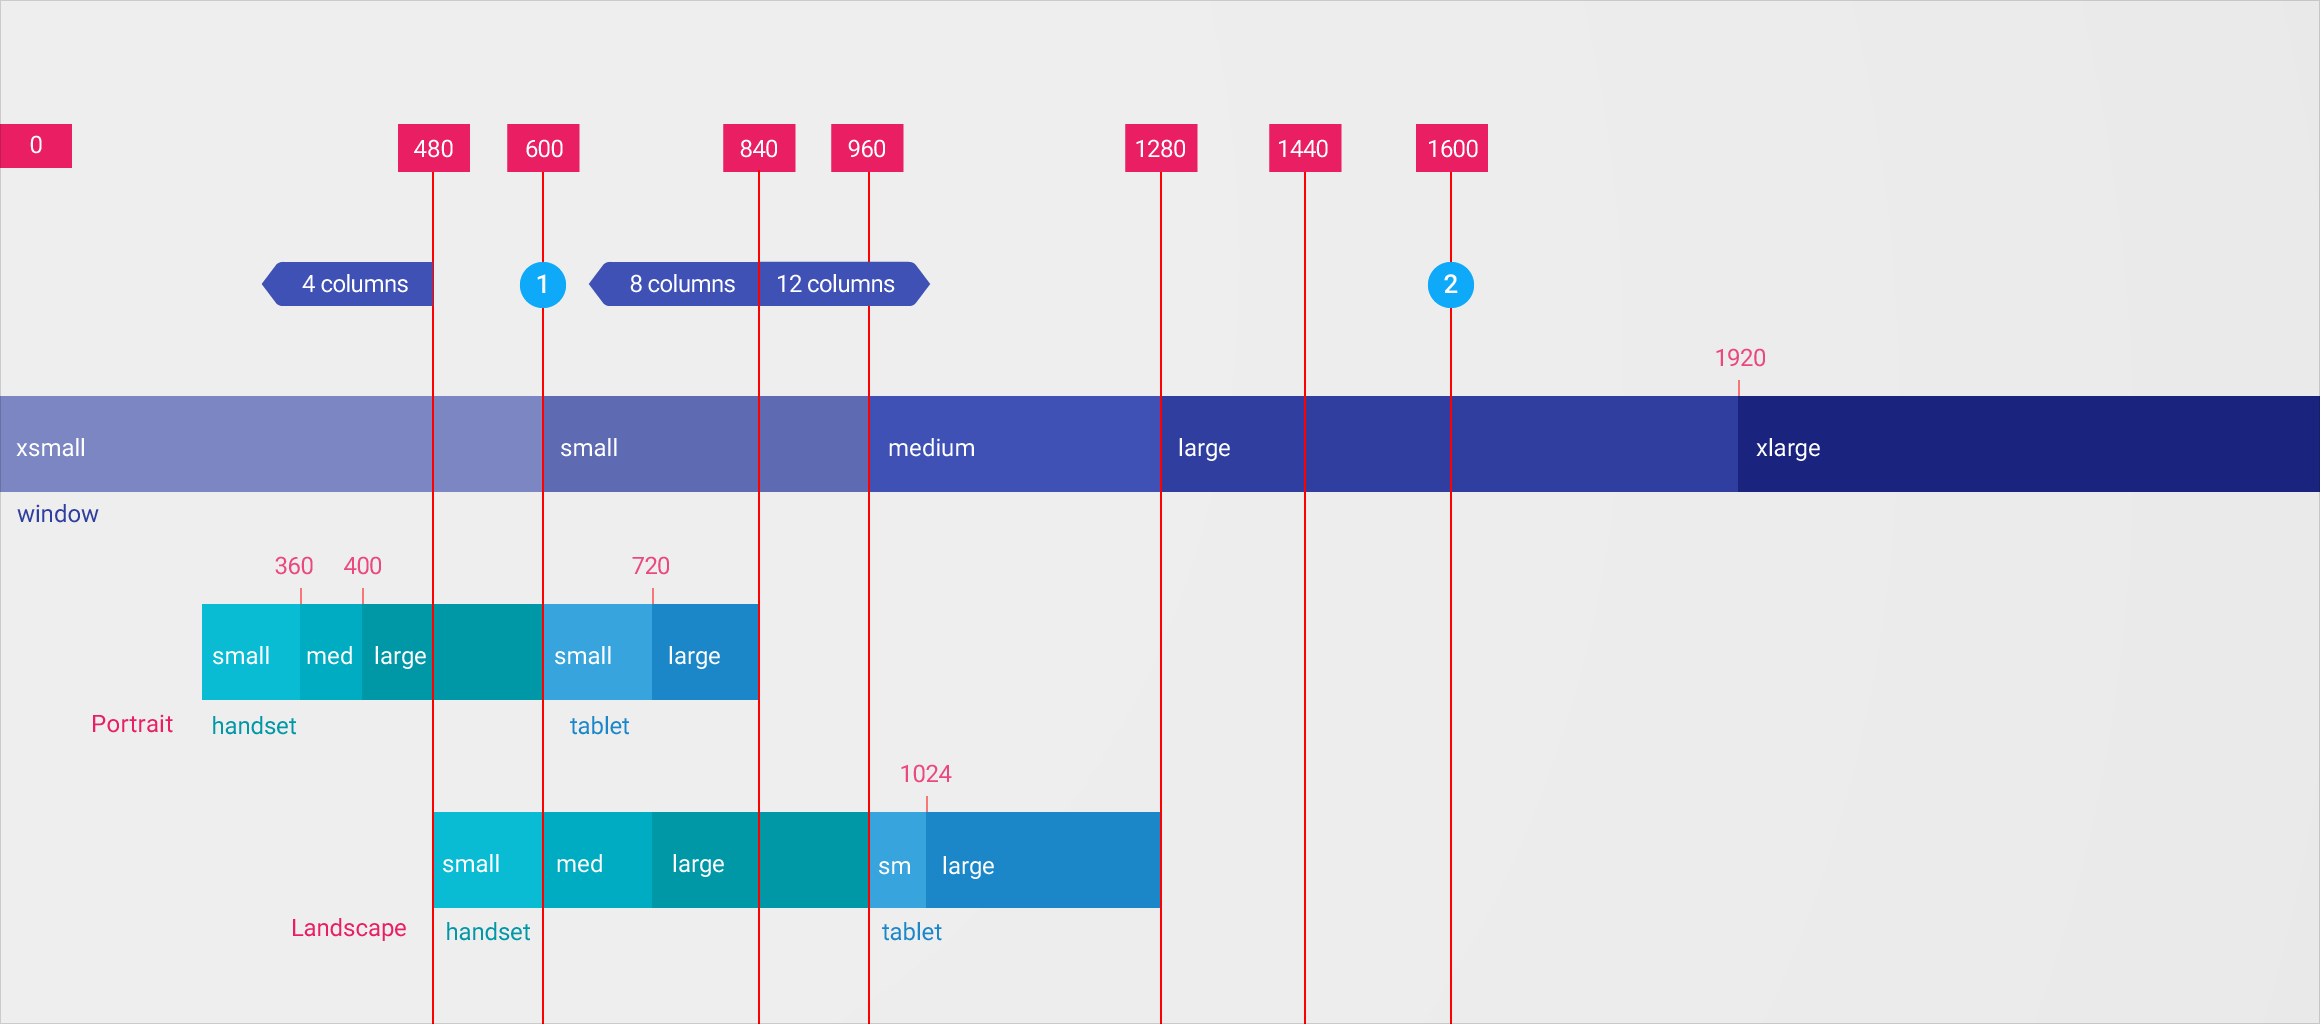
\includegraphics[scale=0.10]{pwa/responsive/layout-adaptive-breakpoints}

\subsection{ Choosing Four Specific Breakpoints }
Even within an enterprise setting, using all the breakpoints specified within
the Material Design specification can be quite a bit. We recommend using the
following breakpoints:

\begin{enumerate}
  \item 400px[Mobile Large - Portrait]
  \item 720px[Tablet Large - Portrait + Mobile Large - Landscape]
  \item 1024px[Tablet Large - Landscape]
  \item 1424px[Desktop Large](16p below 1440 to accommodate for gutter space)
\end{enumerate}

\subsection{ Of Four Breakpoints, Which Designs are Required? }
2 Designs are required, Mobile Large(400px), and Tablet Large(1024px).

\subsection{ Does UX/UI Need to Follow these Breakpoints? }
UX/UI does not need to use actual engineering breakpoints. For instance,
it might be easier to design with a laptop in consideration, instead of a large
tablet.

\subsection{ Build Media Query Function }
Per conventions, it is reccomended that all items relating to the DLS be
specified with regards to functions. That way, we have a way of making sure
that nothing deviates from the design language system.

We will be creating an ill-ui folder and ill.scss file) in our lib folder, to
hold all all of our app's .scss files. In addition, we will be creating an
 \_ill-breakpoints.scss file, to be imported in our ill-ui.scss file. We will be
creating the following in our app:

\begin{lstlisting}
  @function ill-breakpoint($breakpoint) {
  $breakpoints: ('small': 400, 'medium': 720, 'large': 1024,
  'extra-large': 1424);

  @if(index($breakpoints, $breakpoint)) {
    @return #{map-get($breakpoints, breakpoint)}px;
  }
  @else {
    @error "Must contain one of the following strings: #{$breakpoints}.";
  }
}
\end{lstlisting}

Let's imagine you are now building a media query for a specific component
that you are using, you can do something like the following.

\maketitle{}
\section{ PWA Toolset - Physical Devices }

There is currently a formula with which devices to use. Latest regular sized
Iphone, and Iphone Plus. Latest Google Pixel non plus
\footnote{That's right, skip the Samsung.}. Latest Ipad + Ipad Mini. That
is it. These are mostly used as a way to see web in real time, as you are
developing your application.

Therefore, the reccomended Physical mobile devices are as follows:
\begin{enumerate}
  \item Iphone 8
  \item Iphone 8 Plus
  \item Google Pixel 2
  \item Ipad (2018)
  \item Ipad Mini 4
\end{enumerate}

\subsection{ Browser Dependencies }

The following is expected browser dependencies on Desktop:
\begin{enumerate}
  \item latest two Chrome releases
  \item latest two Firefox releases
  \item latest Safari
  \item latest Internet Explorer
  \item latest Internet Explorer
  \item latest Microsoft Edge
  \item Windows 10
  \item Windows 8
  \item macOS Sierra
\end{enumerate}

\subsection{ Testing Local Server on Physical Device }

Now that we have our physical devices that we would like to work on, let's set
up a way that we can test on these mobile devices. Ideally the following three
criteria should be solved:
\begin{enumerate}
  \item Url that remains the same for dev - to be used on mobile device
  \item When edit is made, it should update all mobile devides simultaneously
  \item Have all mobile devices in a central location, so that we can visibly
  see all changes that are being made
  \item synchronized interactions \footnote{Clicking on a button in one place
  change it in all other places.}
\end{enumerate}

\subsection{ Ghost Labs }

First, our winner for responsive testing is Ghost Labs. Ghost labs fulfills all
of the above criteria mentioned above. Going into short why we chose it over
all other contendors:
\begin{enumerate}
  \item Very easy to setup, and therefore removes overhead for initial setup
  \item There isn't anything required to install on different devices. It is
  simply a url that is used, and shared across device.
  \item Screenshots on remote mobile devices
  \item Ghostlab has a built in inspector for debugging
  \item One click workspace, in order to start up all devices once again.
  \item Presentation mode, allowing users to present web app.
\end{enumerate}

\subsubsection{ Setting up Ghost Labs }
First and foremost, buy the Ghost Lab Device Lab Selector. I can assure you, it
is an architectural decision. The whole point behind developing on a physical
mobile/tablet devices, is to improve developer workflow. So that any change that
happens, can be viewed immediatly. The device Lab selector serves that purpose.


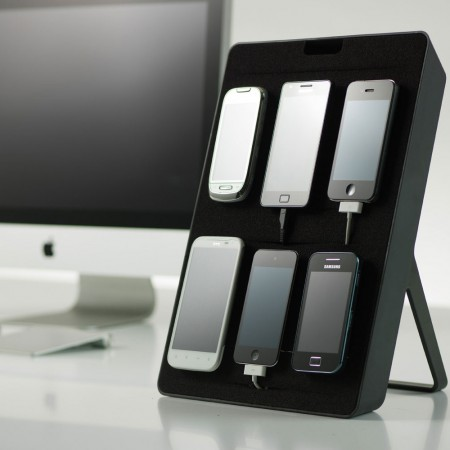
\includegraphics[width=9.1cm, height=6cm]{pwa/pwa-toolset-physical-devices/device-lab-stand}

Setting up ghost labs is as simple as running it in the mac application, and
being able to open on numerous devices. The following is a screenshot of what
you might see in your Ghostlab application:


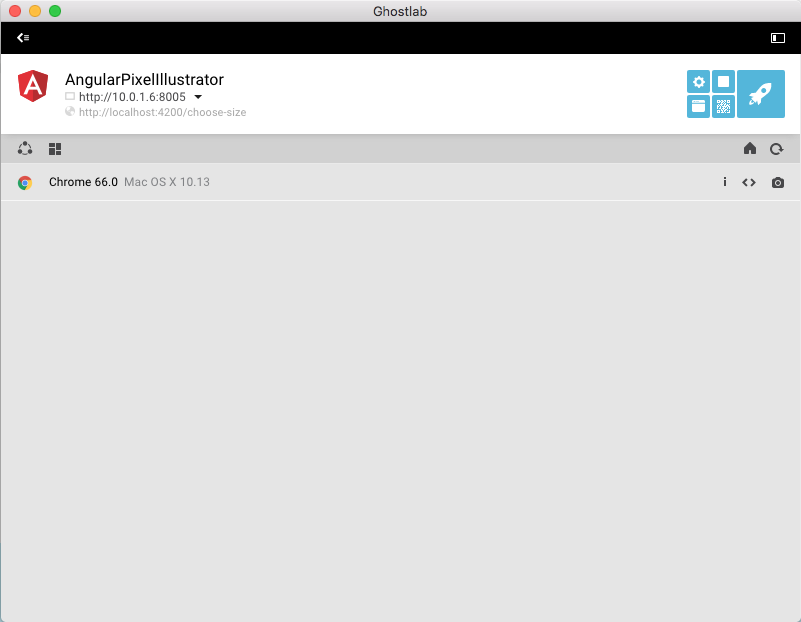
\includegraphics[width=9.1cm, height=6cm]{pwa/pwa-toolset-physical-devices/ghostlabs-screenshot}

Simply drag and drop the url of your browser into application. Click on the play
button. It will open up the above screenshot. You then have the option of
opening up the Ghost Labs generated url in any mobile device, by simply
scanning the qr code.

\subsubsection{ Notable Mentions of Ghost Labs }
\begin{enumerate}
  \item Synchronized browsing between different devices.
  \item Compile and refresh happens as if working with native CLI.
  \item Remote inspection of mobile devices.
  \item Remote screenshots.
\end{enumerate}

\subsubsection{ Final Words on Ghost Labs }
With regards to setting up responsive development workflow, Ghost Labs is next
to none. The \$49 dollar licensing fee is chump change. The amount of time
saved on infrastructure, is worth the investment. The device lab in addition
to buying actual current devices might go up to something in the ballpark of
\$1,000 to \$2,500.

However, this is arguably a fantastic decision. The engineers on your team have
8 hours a day to develop. Many times taken up by meetings, architectural
decisons, corporate events etc. Allowing them to seamlessly develop, without
having to re-configure their browser is a time saver. Perhaps somewhere around
1 hour a week. In addition, it helps promote developer happiness, by making
their life easier. At the end of the day, perhaps for this reason alone, it is
worth it.


\section{ PWA Toolset - Sauce Labs }

\subsection{ The Value of a Continuous Testing Cloud? }

As we have mentioned in the chapter for physical devices, we have quite a bit of
different platforms to work on. Ideally, we want an environment that we can set
up with E2E tests, as well as integration tests, and then run on all environments.
This is on top of the physical devices we already have. To clarify\footnote{i'm saying this a completely friendly way}

The idea of physical devices is as follows: to have a real time update of all
edits being done in your local environment, so that you can go ahead and have a
continuous local development environment.

The idea of a continuous testing cloud, is to be able to check that all devices
and browsers are being properly tested on. This will work strictly with one's
e2e tests.

\subsection{ Bring it to the Table - Why We Chose Sauce Labs }

At this point in time, there are really two main competitors, when it comes
down to continuous cloud computing:

\begin{enumerate}
  \item Sauce Labs
  \item BrowserStack
\end{enumerate}

Before we go into the above, endtest which is a fantastic up and comer, is
unfortunately a victom of it's own business model. While allowing users to
create a very simple version of tests, it also locks in users to it's platform.
There is no way of exporting these tests, and it makes it a very uncomfortable
place for many enterprises. This is precisely the type of application we are
trying to focus on, in this book, so we shall move on. \footnote{Even if I were
working on a small app, I would still not use endtest, for fear of scale}

\subsection{ Sauce Labs }

\includegraphics[scale=0.25]{pwa/pwa-toolset-sauce-labs/logo-sauce-labs}
vs.

\includegraphics[scale=0.4]{pwa/pwa-toolset-sauce-labs/logo-browserstack}

The competition for BrowserStack vs. Sauce Labs is pretty stiff. To be honest,
at this point, they should go for different marketplaces, or one of them should
go under. They have many of the following similar features:
\begin{enumerate}
  \item Platform
  \item Languages Support
  \item Framework
  \item Support
  \item Browser Release Support
  \item Browser Support
\end{enumerate}

However, the following are the reasons why we believe Sauce Labs is the better
choice. Sauce Labs has quite the roster of large clients, and it's fantstic
documentation shows. In addition, because Sauce Labs is widely used, we are able
to find better community support. Channels such as StackOverflow for a specific
quirk.

\subsection{ How to use Sauce Labs }


\chapter{ Mobile First - Building a Progressive Web App }

\section{ Why Build a Progressive Web App? }
When building a an enterprise application, think about building a Progressive
Web App. It will allow your web experience to be built to feel as if it is a
native app experience. Not only will it make it progressive, but it will make
your users feel as if they are a part of an experience that is all encompassing.
It will give them the overencompassing feeling that they are getting the best
experience possible \footnote{We will discuss moving the app over to a native
app soon using NativeScript.}. Swipe right on Progressive Web Apps \footnote{
That is a millenial joke, but also a darn good PWA pun.}.

\section{ The Technical Benefits of a PWA }

\begin{enumerate}
  \item \textbf{Progressive} - Work for every user, regardless of browser choice
  because they’re built with progressive enhancement as a core tenet.
  \item \textbf{Responsive} - Fit any form factor, desktop, mobile, tablet, or
  whatever is next.
  \item \textbf{Connectivity} independent - Enhanced with service workers to work
  offline or on low quality networks.
  \item \textbf{App-like} - Use the app-shell model to provide app-style
  navigations and interactions.
  \item \textbf{Fresh} - Always up-to-date thanks to the service worker update
  process.
  \item \textbf{Safe} - Served via TLS to prevent snooping and ensure content
  hasn’t been tampered with.
  \item \textbf{Discoverable} - Are identifiable as “applications” thanks to W3C
  manifests and service worker registration scope allowing search engines to find them.
  \item \textbf{Re-engageable} - Make re-engagement easy through features like
  push notifications.
  \item \textbf{Installable} - Allow users to “keep” apps they find most useful
  on their home screen without the hassle of an app store.
  \item \textbf{Linkable} - Easily share via URL and not require complex
  installation.
\end{enumerate}
\textit{Kudos to Addy Somani for this List}
\footnote{https://addyosmani.com/blog/getting-started-with-progressive-web-apps/}

We will go into detail in the following chapters, into detail
\section{ Developing a PWA - The Toolset - An Overview}
When Developing Mobile First, there are three tools, which will be particularly
advantageous:
\begin{enumerate}
  \item Physical Mobile Devices \footnote{A moment on which one's it is, that
  you should work on}
  \item Sauce Labs \footnote{Section on why we chose Sauce Labs, over Browser
  Stack}
  \item Chrome Dev Tools \footnote{Section on why we chose Chrome Dev Tools,
  over Firefox}
\end{enumerate}

\section{ Developing a PWA - Software - An Overview}
When developing a PWA, it is important for us to keep in mind, that there will
be specific pieces of software to develop. Of course, there is an official PWA
checklist \footnote{https://developers.google.com/web/progressive-web-apps/checklist}
, but specific technologies, would be as follows: 
\begin{enumerate}
  \item Service Worker
  \item Manifest
  \item Lighthouse
\end{enumerate}

\maketitle{}
\section{ Internationalization }

Internationalization is one of those things that is generally done farther down
the life cycle of an app. "We would like a data table put on every page with
specific data", she says. Only later on i nthe app will having it be
translatable to Frecnh and Mandarin, something that we really want to integrate
within the app.


\chapter{ Creating a component }

For re-iteration purposes, the definition of a component is something consituting
of a larger whole. Ideally anything we can turn into a component in an Angular
environment, will help us. In addition, anything which we can re-use across the
app, is beneficial as well.

When creating components, Angular also makes use of modules. Once again, just to
re-iterate, a module is an independent unit, which is used to construct a larger
interallated construct.

Angular stays true to these two definitions. A component can only be declared by
one component. If it is used by two, or more Angular will complain, saying that it
is already used by another component. Which by definition only constitues a larger whole.
A module on the other hand, is simply an independent unit. If we ever want to use
our component with two components, we will need to include it as part of a module.

Therefore, it is reccomended as general good practice, whenever creating a
component (unless that particular component has children), to always create it
with a module. For other reasons as well, it is smart idea. We will get into
those later \footnote{If you can't wait, and want the full list now, go here to
find it}.

We have already created a component as needed for our router, but for redundancy
sake here are the steps again.

Also, because we will be using sass, let's make sure that our cli is using sass.
Open up the .angular-cli.json file, and change two areas. One:
\begin{verbatim}
  ng set defaults.styleExt scss
\end{verbatim}
This will make it, so that whenever we set up our components using the cli,
again it will be in sass. Second, change your existing styles.css file to
styles.scss.

Let's use the cli to create our first module called choose size.
\begin{verbatim}
  ng g module choose-size
  ng g component choose-size --exports
\end{verbatim}

(The file at this time is included in our app as a route. Let's remove the
default nrwl text from app, so that all we have is choose-size works.)

\section{Architecture time}

Before, we haphazardly created a component in order to introduce routers. Now
that we are going to work on our actual component, let's set aside to specific
items with regards to architecture.

Whenever we want to create a page for our application that will be used as a
route, it is a container. Something which is simply there to "contain" all of
our components. In the root of our app directory we are going to create a
container folder. \footnote{We are once again borrowing from the example-app
project in ngrx/store}

\begin{verbatim}
  mkdir containers
\end{verbatim}
We will also be needing to mention, that we will be
moving our choose-size directory to a newly created components folder.

cd into your containers folder, and create a choose-size-page module/component:
\begin{verbatim}
  ng g module choose-size-page
  ng g component choose-size-page
\end{verbatim}

In this choose-size-page component, we will be adding our choose-size component.

In order to do so, we will need to import the choose-size component in our Angular
app, and add it to our choose-size-page module like so:

\begin{lstlisting}[caption=Importing the choose-size module]
import { ChooseSizeModule } from  '../../components/choose-size/choose-size.module';

@NgModule({
  imports: [
    CommonModule,
    ChooseSizeModule
  ],
  declarations: [ChooseSizePageComponent]
})
\end{lstlisting}

In addition, we are going to want to make sure to add an exports key/value to
our choose-size module, so that by importing it, we have the respective
component available as well.

\begin{lstlisting}[caption=Adding choose-size component as export]
  @NgModule({
   imports: [CommonModule],
   declarations: [ChooseSizeComponent],
   exports: [ChooseSizeComponent]
  })
\end{lstlisting}

With the component module properly imported, we can now use the component in our
choose-size-page html file:
\begin{verbatim}
// choose-size-page.component.html
<app-choose-size></app-choose-size>
\end{verbatim}

\maketitle{}
\section{ Adding a Route to Our Container }

At this point, being that we did not initialize our app with routing
\footnote{So that we may learn as we develop}, we will need to add a routing
file to our app. In our app root, we will be adding an app.routing.module.ts
file.

It will look something like the following:
\begin{lstlisting}[caption=app.routing.module.ts file]
import { NgModule } from '@angular/core';
import { Routes, RouterModule } from '@angular/router';

import { ChooseSizePage } from './containers/choose-size-page/choose-size-page.component';

const routes: Routes = [
  {
    path: '',
    redirectTo: 'choose-size',
    pathMatch: 'full'
  },
  {
    path: 'choose-size',
    component:  ChooseSizePage
  }
];

@NgModule({
  imports: [RouterModule.forRoot(routes)],
  exports: [RouterModule]
})
export class AppRoutingModule { }
\end{lstlisting}

In it, we are redirecting the default path to go to the choose-size url. When
the url switches over to choose-size path, it will load the choose-size component.

We are also obviously going to import the AppRoutingModule in our app.module.ts
file:
\begin{lstlisting}[caption=app.module.ts file]
import { AppRoutingModule } from './app.routing.module';
@NgModule({
  imports: [
    //...
    AppRoutingModule,
    //..
\end{lstlisting}

We are also going to delete the competing:
\begin{lstlisting}[caption=app.module.ts file]
    RouterModule.forRoot(
      [
        {
          path: '',
          redirectTo: 'choose-size',
          pathMatch: 'full'
        },
        {
          path: 'choose-size',
          component: ChooseSizeComponent
        }
      ],
      { initialNavigation: 'enabled' }
    ),
\end{lstlisting}

That we had in our app.module.ts, to tidy up that app a bit.

Terrific, we now have our app by default re-routing to the choose-size url path
and loading the choose-size component. Let's move onto styling real quick next.


\chapter{ Styling a Component }

Styling a component, of course, is a very complex topic. With styling, as an
architect in an Angular setting, there are 4 things that you will have to keep
in mind:
\begin{enumerate}
  \item Pre-processor of choice(Scss, Less, PostCss, etc.)
  \section{ Pre-processor of choice }
  \item Design system
    \begin{enumerate}
      \item Material Design(Google)
      \item Fluent Design(Microsoft)
      \item Flat Design(Apple)
    \end{enumerate}
  \item Responsive design(even if you have a mobile/tablet app)
  \item Naming convention of CSS classes
\end{enumerate}

\section{ Pre-processor of choice }
For our preprocessor, we have chosen Sass. \footnote{Incude link for a
discussion of why that is}

\section{ Naming Convention }
For our naming convention, we will go with BEM. It is an extremely easy way
of setting a part a specific component from an html and css side of things. A
quick primer on BEM.
Block is a component. We will be using pascal casing for ours \footnote{Link to
airbnb style guide}
Element is a child of block. It uses an underscore. For instance:
\begin{verbatim}
<div class = 'ChooseSize__input'></div>
\end{verbatim}
M stands for modifier. A modifier is an element, which modifies an already
existing element.
\begin{verbatim}

\end{verbatim}


\section{ Design System }
In an Angular setting, the component library which seems to make most sense is
Material Components
\footnote{https://material.angular.io/components/categories}. For starters, it
is a complete design system. All component's design will be synonymous with
each other. In addition, it is in the process of creating a cdk, which makes
all of these components customizable. In addition, it is a really nice design,
and feels native to the way Angular works. I have used it versus other libraries
and I can really say the documentation is just fantastic. I have used it in more
complex settings(e.g. the data-table), and adding on new functionality has been
just a joy.

\section{ Adding Material Design to Our App }
First install Angular Material components and Angular Animations to our app.
\begin{verbatim}
  npm install --save @angular/material @angular/cdk
  npm install --save @angular/animations
\end{verbatim}

In addition, we will need to add default styling to our app, in order for
styling to be applied to our Angular Material component. Inside of our
styles.scss file, import the following.
\begin{lstlisting}
@import '~@angular/material/prebuilt-themes/deeppurple-amber.css';
\end{lstlisting}

\section{ Our first component }
In our app, we are going to create our first component. It is essentially a form
with three fields:
\begin{itemize}
  \item Columns
  \item Rows
  \item Pixel Size
\end{itemize}

In addition, there will be a button which will say, 'Create Grid'. We are also
going to wrap our component, with the <mat-card> component, add a width of
300, margin-top and center.

\subsection{ Notable Mention - @HostBinding }
In an angular app, many times, we will want to add a specific class to our
parent container. In our situation, we will be using BEM, and creating a
ChooseSize class. It will implement flex, and use justify content, in order to
center the <mat-card> component.

\begin{lstlisting}[caption=My Javascript Example]
import { Component, HostBinding, OnInit } from '@angular/core';

@Component({
  selector: 'app-choose-size',
  templateUrl: './choose-size.component.html',
  styleUrls: ['./choose-size.component.scss']
})
export class ChooseSizeComponent implements OnInit {
  @HostBinding('class') class = 'ChooseSize';
  constructor() {}

  ngOnInit() {}
}
\end{lstlisting}

By putting @HostBinding as a decorator \footnote{If not familiar with decorator
, it is a function that is run when particular class is called} within our app,
it causes the host class to have the ChooseSize class. We are then able to
target our host element our scss:
\begin{verbatim}
  :host.ChooseSize {
    display: flex;
    justify-content: center;
  }
\end{verbatim}

\section{ CSS Naming Convention }
In your modern day front end framework, such as Angular, generally, we do not
have to worry about clashing namespaces. \footnote{Historal footnote, the
turning point for me was with this article \href{https://glenmaddern.com/articles/css-modules}{here}}.
Many other issues with css at scale, have been solved as well, have been 
solved by the general ecosystem, scss included.

However, reccomended architecture is that one still use something like BEM. I
would like to argue for using BEM in an Angular setting:
\begin{enumerate}
  \item It allows for easy grep in code base, when inspecting element first
  within chrome.
  \item It documents the type of element that it is.
  \item It will give structure to html, without need of using pug, or some other
  html pre-processor.
  \item Ease's creation of classes for integration testing\footnote{Use a modifer
  for BEM}
\end{enumerate}

It should be noted, that within our app, the form has been made a particular
width, which will work on all screen sizes, without the need of adjusting width.
As we move along in our app, we will have the option to look into sitations
wherein we can use actual media queries.

\section{When to Use @ngrx/store}
When to use @ngrx/store can be a very opiniated item to consider. State as we
know it, is a single data object, that can be accessed anywhere within the app.
How this happens, changes from one state management framework to another, but
the core is the same. However, the difficulty, is that state, being that it
exists outside of the component, can contain quite a bit of bloat.

\mybox{It is interesting to note, that the original implementation of Flux
was created by Facebook back in 2014\footnote{This video contains https://www.youtube.com/watch?v=nYkdrAPrdcw this fact}.
It was because they had a bug with regards to the chat counter, that just kept
on coming back. It would mention that a user did not read a message, but that
wasn't true. Flux was the architecture they came up with in order to solve this
bug. It's important to understand the history of where Flux came from, when
trying to understand how to move forward using it. It's important to also
realize, that the issue, wasn't they weren't able to solve it, it is that the
bug kept coming back. Flux solved it, due to it's straight forward way of
solving multiple components interacting with each other.

``It is important to remember, that a store is about creating an in-memory client
side database, which is a user-specific slice of the database, and use that
data to derivce View Models from it on the client.''
}

\subsection{Redux as evolution on Flux}
Redux solved the same problem Flux did. However, it simplified the process.
Without going into too much detail and instead showing a photo, Redux simplified
the problem it solved, and made it easier to implement:

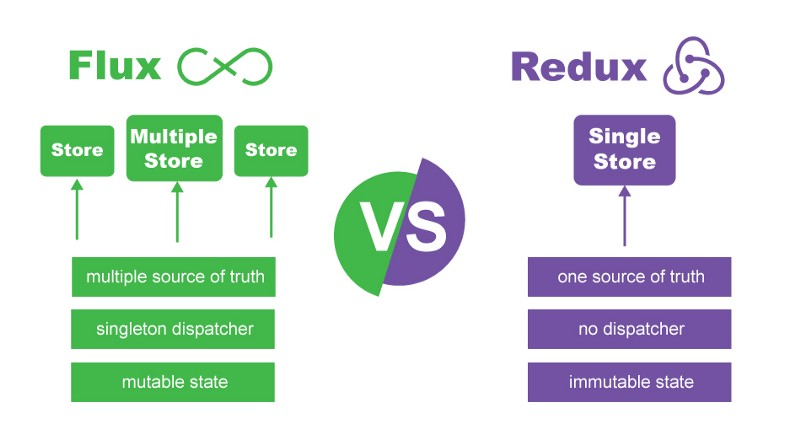
\includegraphics[width=9.1cm, height=6cm]{./state/when-to-use-ngrx/flux_v_redux}

It also more importantly, standardized the Flux architecture as a library.

\subsection{@ngrx/store - Integrated Reactive Programming with the Store}
@ngrx/store took redux one step further, and integrated observables with the
store. There is a fantastic founding paper on the benefits of Real Time
\href{http://www-sop.inria.fr/members/Gerard.Berry/Papers/Berry-IFIP-89.pdf}{Programming}

In it, it discusses two main benefits of Reactive Programming:
\begin{enumerate}
  \item Asynchronous
  \item Detemrinistic
\end{enumerate}

Just to throw out what a quote from who I consider a founder in Reactive
programmin. Andre Staltz when discussing why one should consider Reactive
programming really touches on the core of it all with the following, “Reactive
Programming raises the level of abstraction of your code so you can focus on the interdependence of events that define the business logic…”.
\footnote{https://gist.github.com/staltz/868e7e9bc2a7b8c1f754\#why-should-i-consider-adopting-rp}

That being said, it immediately becomes obvious as to why one would want a
reactive approach towards state. State is generally changed with events, and
being able to abstract the level of state makes complete sense. I cannot stress
how many times, I have been able to pull in an observable using @ngrx/store, and
modify it using rxjs. It greatly abstracts, and simplifies the process.

\mybox{As a side note, ngrx was actually created, to solve performance issues
with change detection in Angular2. It from that point onwards has morphed into
a good idea, allowing the store to be automatically hooked into state:
https://github.com/ngrx/store/issues/16\#issuecomment-172027797}

\subsection{ An Example of an @ngrx/store }

For instance, let's say that we have a user-settings data-access feature. Our
folder file structure might look like the following:

\begin{forest}
  [libs
    [px-illustrator
      [data-access
        [user-settings
          [src
            [lib
              [\_+state
                [\_user-settings.actions.ts,file]
                [\_user-settings.effects.spec.ts,file]
                [\_user-settings.effects.ts,file]
                [\_user-settings.facade.mock.ts,file]
                [\_user-settings.facade.spec.ts,file]
                [\_user-settings.facade.ts,file]
                [\_user-settings.reducer.spec.ts,file]
                [\_user-settings.reducer.ts,file]
                [\_user-settings.selectors.ts,file]
              ]
              [\_px-illustrator-data-access-user-settings.module.ts,file]
              [\_px-illustrator-data-access-user-settings.module.spec.ts,file]
              [\_px-illustrator-data-access-user-settings-testing.module.spec.ts,file]
            ]
            [\_index.ts,file]
            [\_test.ts,file]
          ]
          [\_karma.conf,file]
          [\_README.md,file]
          [\_tsconfig.lib,file]
          [\_tsconfig.lib.json,file]
          [\_tsconfig.spec.json,file]
          [\_tslint.json,file]
        ]
      ]
    ]
  ]
\end{forest}


This, of course, would be in an enterprise setting, which honestly this book
is geared towards. However, it definitely strikes home a very good point. There
is a ton of bloat to creating a store. Even once a developer get's over the hill
of creating state, and get's used to it, it's still a lot to manage, and one
just has to ask, does it always make sense?

\subsection{Understanding the Reality of State}
I think that looking at the above folder/file strucutre, it is very important
to realize that state has gone so far beyond what it was originally intended to
do. You will notice effects, a facade pattern. In addition, quietly sitting
inside of our reducer, is @ngrx/entity. The whole suite of @ngrx is so robust
that it deals with the entire life cycle, of pulling in data, and integrating it
with the client side. In fact, if it wasn't for the bloat that it introduced,
it would be able to solve every single situation, wherein we are trying to carry
over data into the client side, in a scalable, and maintainable fashion. Ok, so
let's deep dive into it.

\subsection{ Addressing the Problems State Alleviates }
First and foremost, I think it would be most effective if we were to directly
jump into the problems that state solves:
\begin{enumerate}
  \item Avoiding Multiple Actors
  \item Avoid Extraneous @Inputs
  \begin{enumerate}
    \item Pass down multiple levels to child, and send change back to parent
    \item Siblings in a tree, might have to pass up and over
  \end{enumerate}
  \item Stops Event Bussing /marginpar{Look more into this one}
  \item Decouples component interaction. Component does not know what changed,
  only knows what changed it.
  \item Allows for Component interaction via the Observable Pattern
  \item Client Side Cache if needed.
  \item Place to Put Temporary UI State
\end{enumerate}

These would be in my humble opinion, the 7 things that state has to offer. If a
component were to be able to interact with another component on that page, by
altering it's data, it should have state.

\subsubsection{ Addressing Additional two Offered by @ngrx/store }
Added into your classic @nrwl/nx ecosystem, is:
\begin{enumerate}
  \item @ngrx/entity
  \item Facade pattern for single
  \item Effects for asynchronous programming
\end{enumerate}

\subsection{The Mesmerism of @ngrx/store}

So, as mentioned before, the @ngrx/store ecosytem has grown into a beast. In
fact, an Angular developer working on an enterprise, data heavy application,
might spend 60\% to 70\%(rough estimate) of their time working within
@ngrx/store. I was a little bit curious as to how this repition might
psychologically affect the way that we as software engineers develop. In
particular, if we can introduce services that accomplish what @ngrx/store does,
albeit less bloat, is it worth it for the team?

I found an interesting book, called, ``On Repeat: How Music Plays the Mind''. It
discusses a very interesting topic, of how we as humans interact with music. In
it, it discusses something known as ``The Exposure Effect''. It's something that
we have all experienced with regards to music. For instance, you will hear some
music on the radio that you are not particularly fond of. However, you will here
it again the grocery store, movie theater, and then the store corner once again!
By this time, you are hooked! More importantly, as the book discusses, as you
are used to the repition of the song, you are already expecting the next piece
of song, by the time you working on the beginning of it. Repition, allows for us
as the book argues, to look at a passage as a whole.

Arguably, the point can be made for software as well. Within the application you
are working on, the more you use that pattern the more accustomed you are to it.
In addition, and I can personally attest to this, by the time, I am working on
the facade, I am already thinking of the effect that is going to tie into our
service, and how I am going to tie it into the component. Jumping out of this
repitition can counter-productive, even if there is less code involved by
creating a service.

\subsection{ Attachments Service - Story Time }
There are some very unique cases, where perhaps state shouldn't be used on an
objective level. I for one always felt that state has a bit of bloat(, albeit my
opinion is beggining to change). However, after discussing with team members,
I have begun to see the way they think. This particular situation was about a
feature for attachments that the app needed. In particular, multiple components
on the same page, would have attachments that would be uploaded to a server.
Then, when the api using the attachment would make a request, it would pull
attachment from the server, using it's id. If a service or @ngrx/store was not
used, there would be alot of repitition across the app. This led to the dillema,
should a service, or @ngrx/store be used.

\subsection{ Business Requirments }
One, is that multiple components on the same page were to use this attachments
service. Second, is that we want to show the user when a certain attachment is
loading, and when it is no longer loading.

\subsection{ Argument for using a Service }
In truth, the attachments were meant to be self contained within a singular
component. This would have made the service as very simple. However, based on
the business requirements, we would have had to create a double nested
correlation id. This means that a double nested correlation id pattern had to be
created. One, to make sure that different components do not affect each other.
Two, the id produced on the front end, is different than the id produced on the
backend. We need to create an id that can be used by both. This is done by
creating a second Uuid, that is nested within the first one. I.e. a dictionary
inside of a dictionary.

So, really in this situation, there is arguably nothing that the store has to
offer. However, what has happened, using ``The Exposure Effect'' is that we are
now comfortable with the API for @ngrx/entity. Comfortable isn't accurate
actually. We are able to predict, @ngrx/store as a whole. Any developer who
worked and will work within the app, can pick up on the code base easier than
a service, beign that it is predictable. In addition, we have a single place
where we expect all of our data to be. Creating a service like this, might make
sense for the person spending the time thinking through the problem. However,
for any other person, it will be an incredibly uncomfortable experience reading
through your code. @ngrx/store therefore at this point takes on it's new life
as a way to make sure code is consistent, even if it isn't the right choice for
your app.

\subsection{ What Comes Out From Our Back and Forth }
Truly, any enterprise situation, wherein a data request is made from the
back end, it should be handled using @ngrx/store and not services. This is
simply because, in any enterprise setting, the majority of situations is more
properly handled using @ngrx/store.
\begin{enumerate}
  \item It allows for a cookie cutter api, that is used time and time again. The
  code bloat it creates, is alleviated by use of Nrwl Nx.
  \item Your application's performance will not affected as a result.
  \item From personal experience, business requirment change quite a bit. The
odds of your service now being needed to re-written to accomodate it being
used in multiple components, is also quite high.
\end{enumerate}

\subsection{ Final Note }
If you are building an enterprise app from the beginning and are building a
team, put this as part of the conventions right away. It will make your life
easier. If you have a team, and you haven't fully agreed on this one, send them
this article and start a conversation. Razroo Cares.


\section{ Primer - Actions }
At this is a definitive guide, and covers all aspects of the framework, one
would be remiss without going through the entire lifecycle of the store, and
mentioning it here.

An action is a function which contains two very important pieces of information:
\begin{enumerate}
  \item What the name(type) of the action is. \footnote{Why this is important we
  will get to soon}
  \item The payload of the action. Which is a single object, containing all the
  data passed into the store.
\end{enumerate}

\subsection{An example of an Action in an Angular setting}
An Action is pretty generic across different frameworks. \footnote{For certain
frameworks, this is less relevant, such as React + Vue.}. However, within an
Angular setting, it means that we are using @ngrx/store for controlling state
across our app and Typescript. Within an Angular setting, an action will look
like the following:
\begin{lstlisting}
export class LoadCodeBox extends Action {
  readonly type = CodeBoxTypes.LoadCode;

  constructor(public payload: {id: string}) { }
}

export class CodeBoxLoaded extends Action {
  readonly type = CodeBoxTypes.LoadCode;

  constructor(public payload: CodeBox) { }
}
\end{lstlisting}

In the above code, is a perfect representation of your classic action. It
contains the type of action. So that in you reducer, or effect(which we will
go into momentarily if not familiar), we can trigger reduce(combine) data passed
in, with data already present.

\mybox{In an Angular/Typescript setting, you will commonly find a general export
type, for the entire app:
  export type Actions = LoadCodeBox | CodeBoxLoaded;

This is usually used within the reducer, and is called a union interface type.
It allows us to combine the type for numerous actions within a single type. We
can then pass this as a type to a reducer, and make sure that we do not
introduce any action beyond that for the particular feature state. It's a great
way to make the develop think twice, if they introduce an action outside of the
feature state into the app.
}

\subsection{An example of using an Action in an Angular setting}
As a matter of philosophy, this book will only introduce how to use something
as it is in the real world. Generally, an action will only be used in a variety
of situations such as an effect, facade, or guard. \footnote{If not familiar, no
need to worry, we will go through this as time goes on.}. As a simple example,
let's use it in a facade \footnote{Something we will discuss, a dedicate an
entire chapter}.

\begin{lstlisting}
  loadCodeBox(id) {
    new LoadCodeBox({id})
  }
\end{lstlisting}

Here we are calling the class by using new. It will call the action whenever the
facade is called.

This would be as simple as a primer can get for actions. It might seem like
there are more questions that came up as a result (Go through potential
questions one might have).

\maketitle{}
\section{ Primer - Reducers }
Reducers are pure functions that take in data \footnote{Should take in data only
and for the sake of this primer, we are going to keep it this way.}, and return
a new data object. Immutability is ideal when using reducers, so that data is
not affected by mistake, when being passed down the pipeline. Reducers tend to
universal across all frameworks, and usually consist of:
\begin{enumerate}
  \item One exported function
  \item A switch:case statement based on action.type
\end{enumerate}

\subsection{ Example of Reducer }
export function reducer(state = initialState, action: book.Actions
| collection.Actions): State {
  switch (action.type) {
    case: CodeBoxActionTypes.CodeBoxLoaded {
      return {
        ids: [ ...codeBoxIds ],
        entities: Object.assign({}, codeBoxEntities),
        selectedCodeBoxId: state.selectedCodeBoxId
      }
    }
    default: {
      return state;
    }
  }
}

This reducer will be called whenever any action is called. However, only if
the action matches the case statement, will the reducer actually run.

\maketitle{}
\section{ History of State Management }

I wanted to write this, because having a history of state management put's into
perspective why we need state management. It also put's into perspective how
much so things change, and how important having a foundation in software is.
In particular, to be aware of alternatives, and to help with learning new
concepts. Jumping right in, Jquery was created a very long time ago, already
back in \href{https://en.wikipedia.org/wiki/JQuery}{2006}. Show, hide, remove,
add, as well as element selectors, were already present in
\href{http://api.jquery.com/category/version/1.0/}{Version 1}. Javascript had
this capability as well if need be. However, no one really thought of it as
state management.

\subsection{ State Management with jQuery }
A classic component, I remember that was always created with Jquery, would be
image sliders. In the more elequent apps, they would use singleton classes,
perhaps \href{https://www.w3schools.com/js/js\_object\_prototypes.asp}{prototypes}
if they knew what they were really doing. Variables would be cached by
initializing once. Functions would be kept small, and everything including css,
would have very unique nomenclature(\href{http://getbem.com/introduction/}{BEMCSS}
for instance). Folder/file structure was important, but there wasn't really
anything like state management. Ironically, many smaller websites at this time
were more performant in many ways. Why? Because, many intentionally kept them
small, in order to do more. 2015-2016 was a great year of performance, due to a
growth spurt in \href{https://chromereleases.googleblog.com/2015/03/stable-channel-update.html}{browser capabilities}.
The change log for 2015, is the last time you will see google chrome mentioning
performance in it's logs.

Just for clarity sake, the following is a great example of how Jquery and
Javascript "state management" would work(updated to use es6). A file which would
contain values, would be used to create/add/delete/update across the app:

\begin{lstlisting}
// _elem.js file
storeValues: [],
storeColors: [],
sassColorVariables: [],
lessColorVariables: []

// _grid.js file
updateGridColor: () => {
  for(let x = 0; x < elem.s.columnCount; x++) {
    for(let y = 0; y < elem.s.rowCount; y++) {
      ctx.strokeStyle = `${elem.el.backgroundRed.value + 44}. ${elem.el.backgroundGreen.value + 44}. ${elem.el.backgroundBlue.value + 44}`;
      ctx.strokeRect(x * elem.s.pixSize, y * elem.s.pixSize, elem.s.pixSize, elem.s.pixSize);
      ctx.fillStyle = elem.el.backgroundHexColor.value;
      ctx.fillRect(x * elem.s.pixSize + 1, y * elem.s.pixSize + 1, elem.s.pixSize - 2, elem.s.pixSize - 2);
    }
  }

  for(let x = 0; x < elem.s.storeValues.length; x++){
    ctx.fillStyle = elem.s.storeValues[x][2];
    ctx.fillRect(parseFloat(elem.s.storeValues[x][0]) + 1, parseFloat(elem.s.storeValues[x][1]) + 1, elem.s.pixSize - 2, elem.s.pixSize - 2);
  }
}

\end{lstlisting}
Above code taken from the \href{codeIllustrator}{https://github.com/CharlieGreenman/codeIllustrator} repo.

\subsection{ State Management with Backbone }
Backbone applications to me were so funny, and still are. It literally looked
like a well architected Jquery app minus routing. Which now that I think about
it, isn't funny. Backbone was a big step up. Routing was a very nice touch that
offered something like that out of the box. Ultimately, there really was no
concept of state management with backbone either. However, I remember apps being
performant, and unmanageable in many cases due to the bad architecture. A step
up, of course from badly engineered Jquery applications. So, no state management
at this point yet, still! However, using model, there was somewhat a way to do
this, that was baked into best practices:

\begin{lstlisting}
  // note_model.js
"use strict";
APP.NoteModel = Backbone.Model.extend({
  // you can set any defaults you would like here
  defaults: {
    title: "",
    description: "",
    author: "",
    // just setting random number for id would set as primary key from server
    id: _.random(0, 10000)
  },
  //...
  // note_edit.js
  save: function (event) {
      event.stopPropagation();
      event.preventDefault();

      // update our model with values from the form
      this.model.set({
        title: this.$el.find('input[name=title]').val(),
        author: this.$el.find('input[name=author]').val(),
        description: this.$el.find('textarea[name=description]').val()
      });
  //...

\end{lstlisting}

This model would global, or per each component, and could be updated using the
above syntax.

\subsection{ State Management with AngularJS }
AngularJS was fantastic because it offered two way binding out of the box. Alot
of web applications need that. It also came hand in hand with Jasmine unit
testing, and event handling. Completely irrelevant to state management. However,
because it introduced services, it really was the first framework to start boxing
applications into, "this is what front end architecture should look like",
paving the way for state management.

Services, while mainly used for data, were also used different parts of the
applciation to interact with each other. Being that Angular applications were
Single Page Applications by default, this worked. State was synonymous with
services. If you wanted different components to know about the data of service,
you would have a setter and getter for that service. The issue with this
approach, is that there would be 4, or 5 services that would interact with each
other, and it would cause serious issues. In addition, in many applications, old
code/bad practices would use \$scope in the code base, causing some serious
perfomance issues. The following is what a sample servic using a factory would
look like:

\begin{lstlisting}
  var myApp = angular.module('myApp',[]);
  myApp.factory('myService', function() {
      var test = 5;
      var obj = {
          test : 5
      }

      return{
        setTestVal: function(val){
          test = val;
          obj.test = val;
        },
        getTestVal: function(){
          return test;
        },
        data : obj
      }


  });

  function MyCtrl($scope, myService) {
      $scope.test = myService.getTestVal();
      $scope.data = myService.data;
  }

  function SetCtrl($scope, myService){
      $scope.newTestVal = '';
      $scope.setTestVal = function(val){
        myService.setTestVal(val)
      }
  }
\end{lstlisting}


\subsection{ State Management with React }
React came around, and interested me atleast for two reasons. It offered
flexibility being a library and not a framework. Second, it was fast in
comparison to AngularJS. Flux came out, and was my first introduction to a
state management system. Redux came out 6 months after Flux already, so
admittedly, I only had a chance to work with Flux for a month, before we already
started moving to Redux. Flux was a bit difficult, and during that month time,
I remember my code reviews being rampant, with don't do this, do that etc.
Shortly after Flux, Redux came around, and for the first time it felt like a
mature state management system came around.

/begin{lstlisting}
// pixel-color-picker.js component
handlePixelColorChange(e){
    const {dispatch} = this.props;
    this.setState({pixelHex: e.target.value}, function(){
        dispatch(PixelColor(this.state.pixelHex));
        dispatch(PixelColorRGB(hexToRgb(this.state.pixelHex).r, hexToRgb(this.state.pixelHex).g, hexToRgb(this.state.pixelHex).b));
    });
// control-panel.js actions
export function PixelColor(color){
  return{
    type: types.PIXEL\_COLOR,
    pixelHex: color
  }
}

// colorPicker.js reducer
case types.PIXEL\_COLOR:
  return Object.assign({}, state, {
    pixelHex: action.pixelHex || state.pixelHex
  });
/end{lstlisting}

// code take from \href{https://github.com/CharlieGreenman/pixelLight}{here}

\subsection{ Reactive State Management with React and Angular }
Around this time @ngrx/store came out, reactive programming became more popular.
Within the context of state, this meant redux-observable for React, and
@ngrx/store for Angular. For Angular, this meant that state is now cookie
cutter. For React and Angular, it meant that users have the ability to tie state into the
rest of their application.

/begin{lstlisting}
Observable.merge(
  // Create observable map for  when background hex changes, and use that
  // value to update store for backgroundColor
  this.changePixelColor$.map((value: any) => (
    PixelColor(value)
  )),
  this.changePixelColorRGB$.map((value: any) => (
    PixelColorRGB(value.pixelRed, value.pixelGreen,
      value.pixelBlue)
  ))
)
.subscribe((action)=>{
  store.dispatch(action)
})
}
/end{lstlisting}

// code take from \href{https://github.com/CharlieGreenman/angularPixel_illustrator}{here}

\subsection{ Hooks and Context with React + Vue }
Where we are at currently, is that new waves are being made with regards to
state management. State is being baked into frameworks in ways that make it
more lightweight, and easier to deal with. Vue and React now have a feature
called hooks, and context. These allow an app to have state out of the box.
Redux + Redux Observable still have they're place. There are times where state
is neccesary to allow components on different pages interact with each other.
Other times, it can be a way of managing the data, to make sure the app is
maintanable. If you see your app heading in the direction of the latter. Redux +
Redux Observable is still reccomended.

\begin{lstlisting}
// theme-context.js

// Make sure the shape of the default value passed to
// createContext matches the shape that the consumers expect!
export const ThemeContext = React.createContext({
  theme: themes.dark,
  toggleTheme: () => {},
});

// theme-toggler-button.js

import {ThemeContext} from './theme-context';

function ThemeTogglerButton() {
  // The Theme Toggler Button receives not only the theme
  // but also a toggleTheme function from the context
  return (
    <ThemeContext.Consumer>
      {({theme, toggleTheme}) => (
        <button
          onClick={toggleTheme}
          style={{backgroundColor: theme.background}}>
          Toggle Theme
        </button>
      )}
    </ThemeContext.Consumer>
  );
}

export default ThemeTogglerButton;
\end{lstlisting}
code take from \href{https://reactjs.org/docs/context.html}{here}

\subsection{ Final Words on State Management }
One point I would like to end off on. I remember 5 years when all of the
framworks were coming out, there was a developer who told me that if you know
what you are doing, really none of the frameworks are neccesary. That being said,
no one in their right mind, is going to create their own framework when they have
it readily availalble. That is unless the company has the agenda to make one.
However, what is important, is to understand the internals, so that you can
that much more valuable when it comes to performance, and mainatanability of
your project. I think that is obvious, but just wanted to bring it up.

\maketitle{}
\section{ Introduction to @ngrx/store }

As discussed in the chapter on the History of State Management, there has
been quite a series of progression with regards to state management. Redux, is
the mature concept of state management including actions, reducers, and a single
application store. \footnote{This is a footnote for more information on state management}.
Angular's @ngrx/store, which is not front and center, is where redux meets Rxjs.
Rxjs is the Javascript library for using observables
\footnote{More on Observables can be read here}.

\subsection{What Makes @ngrx/store Different than Redux?}
When considering this question, it is more important to consider what is
reactive programming. Reactive programming in particular introduces two concepts
\footnote{http://www-sop.inria.fr/members/Gerard.Berry/Papers/Berry-IFIP-89.pdf}:

\begin{enumerate}
  \item Asynchronous \footnote{Meaning one event fires after the previous one is
  complete, unlike synchronous which means they all fire at the same time, and
  might complete out of order.}
  \item Deterministic \footnote{Always produces the same results. As a side
  effect of this, code becomes very much so cookie cutter, which is great in
  an enterprise setting, as it allows for greater re-use.}
\end{enumerate}

\subsubsection{Asynchronous}
With regards to asynchronous programming, observables are not neccesarily 
reactive in the strictest sense. This is because the client is working 
separate from the server. Events with observables are most definitely reactive
, and help, but many applications are data heavy, and the immediate value of
observables are cut short. In addition, actual UI events from a browser 
perspective are put in a call stack, and are asynchronous by nature. What 
does help, is that baked into the framework is effects. Which does allow the
UI to be asynchronous, but it's not like it's anything crazy. This is 
something which could easily be done with promises. However, @ngrx/store does
tie it nicely into the store as a whole, allowing client state management, 
without going into detail.

\subsubsection{Deterministic}
With regards to determinstic, this generally means in computer science, that
with one particular input, you will alwyas have the same output. However, when
the term is used loosely, it generally means that the code is cookie cutter.
That is, that it can be re-used time and time again.

\subsection{Wrapping Up}
This is really what @ngrx/store tries to produce over other frameworks. It
offers the ability to re-use patterns time and time again. In addition, by
hooking it into the Rxjs lifecycle by using observables it allows patterns and
for code to be cookie cutter. This is really the beauty of @ngrx/store, is that
it offers a end to end solution to for state management. In particular, in the
form of effects, and observables.


\section{ Ngrx CLI }

Of one of the better reccomendations I can give with regards to using Angular
within you app, is using the Nrwl Nx cli. If you are using Nrwl Nx already,
which you should, and have a mono repo setup within your organization, then
it should be readily available. If you haven't already, please refer to the
chapter on Nrwl Nx setting it up.

\subsection{ Why Use a CLI? }
One of the benefits of using a CLI, is that it subtly enforces the entire
team to use a particular convention. With the Nx CLI for ngrx, this is doubly
true, as it strongly enforces conventions to be used as to how ngrx works. In
addition, within the ngrx arena, it strongly enforces how certain files should
be built.

\subsection{ Why use a CLI for ngrx }
Without a doubt the most fustrating thing about Angular before the CLI came
around, is the amount of boilerplate that would be required in order to work
with Angular \footnote{As an example, having to create a scss + html + action +
reducer + effect and respective spec file for each next component created }.
The Nrwl Nx for the most part solves this. In addition, there is much more that
can be done on top of this in the future. Think of automatically generating code
based on instance, but I digress.

\subsection{The two stages of Nx ngrx cli}
There are going to be two stages with regards to using the Nx ngrx cli. One of
them is to create root state. This is going to be empty, and it is just there to
hold the feature reducers of the rest of the app. The 2nd stage, which will be
repeated time and time again, is creating a feature reducer. (Creating a root
reducer is something that you would only have to worry about if you are the one
responsible for creating the project for the first time). I think it would
beneficial to running through the steps of how you would create state with the
@ngrx/cli, if you are not familiar with it already.

\subsection{Creating a Root State}
\mybox{At this point, the Definitive Guide assumes that you have already setup
your space as an Nx Workspace. If you haven't please do. It will not negatively
impact your app in any which way, and will only positively improve the way your
codebase works and your day to day happiness.}

The whole idea of state in ngrx/store, is that there is a single object, and
all subsequent pieces of state are sub piece of state. Therefore all pieces of
state will be contained in a single object. In order to have this done in your
code, you will need to set up state for your root, so that subsequent peices of
state can be added as child object(feature), to the root state. This will only
have to be done once.

In order to create a root reducer:
\begin{lstlisting}[language=Bash]
  ng generate ngrx app --module=apps/<app-name>/src/app/app.module.ts --onlyEmptyRoot
\end{lstlisting}

Note, we have passed in the flag for onlyEmptyRoot, so that none of the files
for actions, reducers, and effects are created. We simply want a module
generated that we can use to import other modules for state.

This will produce the following files /marginpar{Re-visit when we get back to
the app}

\subsection{Creating Feature State}
\mybox{We will be going into detail, into when one should create feature state
management, versus using a service. Or, when it might be considered overkill, or
suprisingly the right thing to do. Please refer to the chapter on data access
architecture, to learn more about when would be the proper time to generate
state for your component.}


\begin{enumerate}
  \item libs/<libname>/src/+state/products.actions.ts
  \item libs/<libname>/src/+state/products.effects.ts
  \item libs/<libname>/src/+state/products.effects.spec.ts
  \item libs/<libname>/src/+state/products.reducer.ts
  \item libs/<libname>/src/+state/products.reducer.spec.ts
\end{enumerate}

There is also the option to add a facade, which is highly reccomended. In
addition, creating a seperate selector file is extremely valuable.


\section{ State Management - @ngrx/store }

Ngrx/store is a layer on top of Redux. It is a state management tool that was
originally created, in order to solve two way binding performance issues within
Angular. \footnote{Need to further bring source for this one}. It then extended
as a way to bring redux natively to Angular, with the use of Observables.

Let's dive into integrating @ngrx/store into our app. 
\mybox{This particular component has been written in the fashion of TDD. 
However, another chapter will be dedicated to TDD/BDD in order to specify
this point specifically.}

\subsection{ Using nx ngrx to Generate State }

\subsubsection{ Create root state using nx ngrx }

First we are going to generate an empty root, for our StoreModule, as well as
our EffectsModule. Our StoreModule is responsible as a singular store object,
which will be holding all of store data. Our EffectsModule is a singular effects
object, which will be holding all of our effects. \footnote{We will discuss
effects in more detail later}

\begin{lstlisting}[language=Bash]
ng generate ngrx app --module=apps/angular-pixel-illustrator/src/app/app.module.ts --onlyEmptyRoot
\end{lstlisting}

\subsubsection{ Create component state using nx ngrx }

Next, we are going to create state for our choose-size component. This is done
with ease using nx ngrx \footnote{Trust me, I've been in situations where I
was not using a CLI. It is not good news}

Run the following command:
\begin{lstlisting}[language=Bash]
ng generate ngrx choose-size --module=apps/angular-pixel-illustrator/src/app/components/choose-size/choose-size.module.ts
\end{lstlisting}

This will generate the following files:
\begin{lstlisting}[language=Bash]
create apps/angular-pixel-illustrator/src/app/components/choose-size/+state/choose-size.actions.ts (684 bytes)
create apps/angular-pixel-illustrator/src/app/components/choose-size/+state/choose-size.reducer.ts (869 bytes)
create apps/angular-pixel-illustrator/src/app/components/choose-size/+state/choose-size.effects.ts (859 bytes)
create apps/angular-pixel-illustrator/src/app/components/choose-size/+state/choose-size.effects.spec.ts (1070 bytes)
create apps/angular-pixel-illustrator/src/app/components/choose-size/+state/choose-size.reducer.spec.ts (364 bytes)
\end{lstlisting}
And update the choose-size module,
\begin{lstlisting}[language=Bash]
update apps/angular-pixel-illustrator/src/app/components/choose-size/choose-size.module.ts
\end{lstlisting}

\subsubsection{ High level overview of nx ngrx }
So, you might be wondering, what do those files that nx ngrx generated actually
do? It will generate three files:
\begin{enumerate}
  \item Action
  \item Reducer
  \item Effect
\end{enumerate}

In addition, nx will add Typescript enums for the action types. It will also
add a respective spec file(unit testing) for the action + reducer file.

\colorbox{darkgray}{\color{white}{Unit testing Actions?}}

Unit testing an action, would simply say, when an action is dispatched, expect
it to be of a certain type. However, enums, as well as type checking, fulfills
that obligation. Therefore, if one is using Typescript along with enums, there
should be no reason for writing unit tests.

\subsubsection{ Installing Redux Dev Tools }
A state environment is incomplete without proper devtools. In particular, being
able to see an action fired, as well as the complete state of any given time,
is invaluable.

Google, "redux Devtools"\footnote{In a book format, in my humble opinion, more
valuable than a link}. It is offered by remotedev.io.

With the chooseSize ngrx nx command, we just made, you should see something like
this:

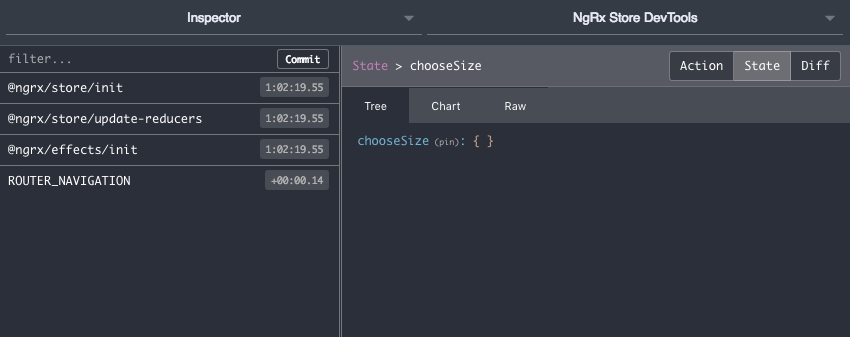
\includegraphics[width=13cm, height=9cm]{state/ngrx-store/redux-store}

\maketitle{}
\section{ What is ngrx/router-store? }

NgRx is an Angular module that leverages RxJS -  a reactive programming library
that deals with the management of data streams and propagation of change. It is
time bound, meaning that data tracking and histories are stored for referencing
and tracing.

Under the traditional model, data is decentralized and sits on each routing
state. This means that if the route changes, history of that data is lost. There
is no past and future states, only the present and navigating away discards any
memory of such occurrences. This can become quite a challenge to keep track of
everything in medium to larger sized applications, especially when navigation
is expected to occur in high frequency.

NgRx solves this issue and provides a solution by creating a central storage
space. It keeps all your current application’s data in one space – turning parts
of your browser’s memory into a  storage bucket for all your data where all
mutations occur only through explicit dispatch actions known as reducers and
becomes the application’s single source of truth. It allows for your
application’s events to exist in a unified manner rather than decentralized
across different parts, children, siblings, partials, factories and routes.

router-store, specifically, is the portion of NgRx module that allows for
listeners to be used for routing actions, meaning that data is allowed to be
stored, shared, consumed and mutated based on the routing status from
a single source. ngrx/router-store, in a way, is like an in-memory database
for your application’s route related data.

\subsection{Why do we need it?}
When data is decentralized and exists on the fly, it becomes prone to errors due
to a lack of history tracking and mutations can occur from different directions.
Duplications can accidentally happen as we try to replicate certain data in
different states and parts of the application.

When relying on Angular’s routing system, we rely on data persistence through
params from navigation/router state. If a child or sibling component requires
that data, it becomes coupled with the parent and data needs to be presented
again in order to be consumed. While factory patterns may solve this issue, it
can quickly get messy if external entry is granted without explicit knowledge.

In larger teams, factory patterns may not be enough to control the flow and
history of data and human error may introduce inconsistencies in the code.

ngRx solves this, along with the reduction of time and code overheads needed to
create factory patterns and singular storage spaces. The library comes ready to
be plugged into any Angular application with its own set of Redux inspired
approach to centralized state storage. Each cycle in a router-store captures a
snapshot of the route’s state and its associated data. When data is decoupled
from routing, it allows your application to become more agile and less dependent
on data states through route params.

\subsection{How to install router store}
Once you have your Angular app, you can use npm to install router-store by using the following commands:

\begin{verbatim}
Npm install @ngrx/router-store –save
\end{verbatim}

If you’re using yarn:
\begin{verbatim}
Yarn add @ngrx/router-store
\end{verbatim}

If you’re project is created with Angular CLI version 6+, you can use the
following command:

\begin{verbatim}
ng add @ngrx/router-store
\end{verbatim}

To check your Angular CLI version, use the following command:
\begin{verbatim}
ng --version
\end{verbatim}

To use inside your application, you’ll need to import the StoreRouterConectingModule and routerReducer from @ngrx/router-store like so:

\begin{verbatim}
import { StoreRouterConnectingModule, routerReducer } from '@ngrx/router-store';
\end{verbatim}

\subsection{Router actions and why they might be useful}
An action is anything that you can do to your application. A router action is an
event that can occur against a specific route on your Angular app. When it comes
to routing, are 5 specific actions that can occur and they are the request, the
action of navigation, the aftermath (also known as navigated), cancellation and
navigation error.

Being able to access and track these actions allows you to control the flow of
route state storage management, access to data and the life cycle process. When
used in conjunction with route guards – a feature that allows you to protect
your views from rendering when there isn’t enough information or the right
access permissions – router actions can help with the resolutions of states and
its consumption.

A request action always kickstart the process which then runs the navigation
action that determines if the dispatch should occur or not. If guards are valid,
a successful navigation will occur and result in a router navigated action. If
something went wrong due to exceptions or lack of user permissions, the router
action will return a \texttt{ROUTER\_CANCEL} action and nullify any attempts to
access the route.

A \texttt{ROUTER\_ERROR} action may occur during the navigation life cycle and
returns the stored state before navigation occurred. This is particularly useful
as it allows the application to back track its action and restore its former
data – a sort of back button without the need for extra configuration or call
to the router state bucket.

\subsection{How to use a custom serializer}

A custom serializer prevents the mutation of snapshot data during the dispatch
process. As data during the navigation cycle is prone to mutability, a custom
serializer returns only what you need to be added to the payload and store. So
in essence, it tracks the difference and change of a particular state without
modifying the entire stored state snapshot.

A custom serializer can be implemented through the abstract class
RouterStateSerializer. It is, in a way, a middleman class that processes the
difference between what the current state is, what is to be changed and updates
only what is necessary.

To create a custom serializer, you’ll need to import Params and
RouterStateSnapshot from @angular/router, along with RouterStateSerializer from
@ngrx/router-store
\begin{verbatim}
import { Params, RouterStateSnapshot } from '@angular/router';
import { RouterStateSerializer } from '@ngrx/router-store';
\end{verbatim}

To create a custom serializer, export a class that implements
RouterStateSerializer with an interface to ensure object uniformity.

Using the serialize() method to convert the state object into a unified format
that conforms to your application’s requirements. This often comes in the form
of mapping router state values to a predefined interface that may look something
like this:

\begin{lstlisting}
//to be used by the serialization process
export interface RouterStateUrl {
  url: string;
  params: Params;
  queryParams: Params;
}
\end{lstlisting}

The CustomSerializer class that implements the imported RouterStateSerializer
using the RouterStateUrl interface created.

\begin{lstlisting}
export class CustomSerializer implements RouterStateSerializer<RouterStateUrl> {
   //serialization code here
}
\end{lstlisting}

Set up the serialization method to return a uniformed set of parameters based
on the template set in the RouterStateUrl interface.

\begin{lstlisting}
serialize(routerState: RouterStateSnapshot): RouterStateUrl {
    let route = routerState.root;

    while (route.firstChild) {
      route = route.firstChild;
    }

    const {
      url,
      root: { queryParams },
    } = routerState;
    const { params } = route;

    // returning the object based on the RouterStateUrl interface
    return { url, params, queryParams };
  }

\end{lstlisting}

To use the custom serializer, implement it inside your @NgModule and call your
exported CustomSerializer class inside the StoreRouterConnectingModule.

\begin{lstlisting}
@NgModule({
  imports: [
    StoreModule.forRoot(reducers),
    RouterModule.forRoot([
      // routes
    ]),
    StoreRouterConnectingModule.forRoot({
      serializer: CustomSerializer,
    }),
  ],
})
\end{lstlisting}

\subsection{Benefits of using router-store with ngrx/store-freeze}
\texttt{ngrx/store-freeze} is a dev tool that can be used during the development
phase of an Angular application to prevent state mutation when using
\texttt{router-store}. It sits on top of \texttt{router-store} as meta data that
acts as an insurance against changes in state data during the process of
transfer to state storage.

As \texttt{router-store} provides snapshots of the \texttt{RouterState} during
the navigation life cycle, it is vital that snapshots passed do not change
during the process of dispatch as this will result the store cycle’s truthiness
breaking due to inaccurate snapshot data.

While serialization already prevents this, \texttt{store-freeze} acts as an
additional safeguard with exceptions thrown when mutations do occur at runtime.
It automatically \emph{`deep freezes'} the entire store state object and
dispatch actions, resulting in a read only effect before it gets passed to the
serializer. This allows errors to be caught before it gets dispatched,
serialized and passed into storage.

\maketitle{}
\section{ Store Selectors }

Selectors are pure functions /footnote{pure function in case you are not aware
of already, are functions which always return the same result, given a certain
parameter} that take slices of state as arguments and return some state data
that we can pass to our components.

\maketitle{}
\section{ Aggregation Pattern }

Many times within any web setting, numerous apis will be feeding into a singular
request. An example would be in an e-commerce setting wherein data for a
particular item, might come from numerous locations. The data for the pants
might come from one api, the analytics api might update, and then a third api
along the lines of data persistence will be called at that time as well.

In a backend setting, usually we try and keep a singular api request for the
business logic of a particular use case. However, there are many times wherein
this will be beyond the power of the developer. In can be in antiquated apis,
or in unique use cases.

\subsection{ The Unique Challenge with Ngrx/effects}
In an ngrx/effects use case, when a user is hitting a single service, and
returning a single action, it is relatively straight forward. This will look
something like the following:
\begin{lstlisting}
@Effect()
getProductInformation$ = this.dataPersistence.fetch(
  ProductTypes.getProductInformation, {
  run: (action: GetProductInformation, state: ProductModelState) => {
    const { userId, productId } = action.payload;

    return this.service
      .getProductInformation(userId, productId)
      .pipe(
        map((product: Product) => new ProductLoaded(product))
      );
  },

  onError: (action: GetProductInformation, error) => {
    console.error('Error', error);
  },
});
\end{lstlisting}

In this example we fire off a service, and return the data from that one
service. We might even have the option to turn the map into a switchMap, that
can be used for numerous actions, originating from a singular service. However,
it immediatly becomes a problem once we start to have a singular effect call
numerous services, wherein one action is expected to have all of it's data.

\subsection{Using the Aggregator Pattern}

\mybox{Before we introduce the aggregator pattern, it is important to note that
in any situation wherein we have numerous actions potentially being dispatched
we are going to want to include a correlation id within our app.}

\maketitle{}
\section{ Re-using Reducer Logic }

In an Angular setting, when using side effects heavily for one's app, 


\chapter{ Ngrx Effects }

\section{Ngrx Effects - A Primer}
Ngrx effects can be one of the more ambigious parts of the ngrx stack. They are
by definitition something that is supposed to happen when something else has
happened. It will listen for a particular action, and true to Ngrx, return an
observable. In this observable one will have the option to do whatever they want
as well as publish(return) to the action stream.

The line, however, can be blurred, however, as to what the difference is between
an ngrx/effect and a ngrx/store. It is therefore important to distinguish for
architectural reasons. In addition, it can be difficult to determine the
different use cases wherein someone would use an effect. It can indeed be a
slippery slope wherein when to use an effect.

\subsection{ Code Example }
\begin{lstlisting}
@Effect({ dispatch: false })
 userDeleted$ = this.dataPersistence.fetch(
   UserActivitiesTypes.UserDeleted,
   {
     run: (action: UserDeleted, state: UserStateModelState) => {
       this.snackBar.open('User Deleted', 'Ok', {
         duration: 2000,
         verticalPosition: 'top',
       });

       return null;
     },

     onError: (action: ActivityDeleted, error) => {
       console.error('Error', error);
     },
   }
 );
\end{lstlisting}

This code example, is a great example as to when someone might use an effect.
As we can see here, we have an action that is being triggered for when a user is
deleted. We then have an effect who's sole purpose to have a snack bar open
when action is called.

\subsection{ The Three Pillars of an Effect }
As we discussed earlier, knowing when to use an effect can be a tricky thing to
decipher. Think of it as having the ability to do the following:
\begin{enumerate}
  \item Hook into State.
  \item Ability to do whatever when action is called.
  \item Publish an action back into the state management cycle.
\end{enumerate}

In our scenario, for deleting a user we had two effects:

We called a GraphQL service to delete a user. We then retrieve the result
returned by the GraphQL service, and trigger another effect, which is our
snackbar effect. Yes, this logic can potentially be handled by our view layer
within our component. In addition, we can use the service directly. However,
having all of this logic encapsulated in our effect makes everything very
clean.

\subsection{ Further Reading }
While this is out of the scope for this book, I would like to suggest further
reading. Naturally, they would be articles that I would discuss on:
\begin{itemize}
  \item Use cases for using Effects.
  \item Use cases for NOT using Effects.
\end{itemize}

The article for use cases with regards to using effects is \href{"Understanding NgRx
Effects and the Action Stream"}{https://medium.com/@tanya/understanding-ngrx-effects-and-the-action-stream-1a74996a0c1c}.
The articl with regards to use cases in which NOT to use effects is
\href{Stop using ngrx/effects for that}{https://medium.com/@m3po22/stop-using-ngrx-effects-for-that-a6ccfe186399}
These two articles along with the information from this chapter. You should be
well along your way for architecting solid ngrx/effects. I personally do not
have patience for the article on, "Stop Using Ngrx effects for That". However,
it is nonetheless the best article on the topic, if you can swallow it.

\maketitle{}
\section{ The Case for Heavily Using Ngrx/entity }
Ngrx/entity for me personally, is the most exciting part of ngrx/entity. Simply
because it is a library based on comp sci fundementals of building an ngrx/store
database. In SQL databases, there is a concept of database normalization. For
instance, let's imagine we have a set of data. In our table, and we would like
to retrieve data from it. The data in JSON formate can look something like this:
\begin{lstlisting}
  interface codeBox {
    id: string;
    color: string;
    xPosition: number;
    yPosition: number;
  }
\end{lstlisting}

Now, let's imagine we have a an array of these codeBox types that we would like
use, that look something like this:
\begin{lstlisting}
  interface codeBoxCollection {
    codebox: codeBox[]
  }
\end{lstlisting}

Now this means, that if we want to select a certain piece of data within our
database table, things can be a little bit tricky. In order to access, for
instance, a certain section of our table, we would need to loop through all of
the data, and then find the appropriate set of data with id that we want.

Instead, what would make out data table more efficient, is if we have a table
of ids that corresponds directly to our table of data. 

\maketitle{}
\section{ Ngrx Entity }

The Ngrx repo until recently had many similar functionalities to your regular
redux app. It included actions, reducers, selectors. However, there has been
efforts to go ahead and create libraries for aspects of ngrx that can perhaps
be re-usable. One of these is ngrx entities.

\subsection{ Ngrx Entity at a High Level }
At it's core, ngrx entity is an API for manipulating and querying entity
collections. In particular:
\begin{enumerate}
  \item Reduce boilerplate for creating reducers that manage a collection of
  models.
  \item Providing performant CRUD operations for managing entity collections.
  \item Extensible type-safe adapters for selecting entity information.
\end{enumerate}

This architecture works really well when creating data as a single source of
truth. For instance, let's say in your application, you have a data table on
every page that pulls in data. Throughout every page, you have a way of
manipulating this data. Using ngrx/entity will allow for this architecture to
be fluid, and have all manipulation of data be within a singular area.

\subsection{ Example of Ngrx Entity }
Within our app we the ability to illustrate a pixelated charachter using pixels.
Every time that a pixel within the grid is selected, we are going to add it to
our store. This store is going to be used to display the code version of the
app. In addition, we are going to have to remove the pixel when clicked on
within our store. In addition, if we have selected a new color, and we select a
new pixel with that color, that pixel should be updated with the proper color.
What we have just described is a perfect CRUD app.

\subsection{ Installing ngrx/enity }
\begin{verbatim}
  npm install @ngrx/entity --save
\end{verbatim}

\subsection{ ngrx/entity - A Step Back }
Let's step back for the time being and look into what ngrx/entity actually does.
Ngrx/entity will create a list of ids and a dictionary of entities. Let's brush
up on entity, list, and dictionary:
\mybox{
entity: In relation to a database , an entity is a single person, place, or
thing about which data can be stored.\footnote{https://whatis.techtarget.com/definition/entity}

List: AKA an array.

Dictionary: Collection which is unordered, changeable and indexed.
}

That being said, a sample ngrx/entity data structure will look like this:
\begin{lstlisting}
  ids: [
    '3QOZBAAAQBAJ',
    'y4nmOe0-WD0C',
    'lS5SAQAAIAAJ',
  ],
  entitites: {
    '3QOZBAAAQBAJ': {
      name: 'Lebron',
      id: '3QOZBAAAQBAJ'
    },
    'y4nmOe0-WD0C': {
      name: 'Kyle',
      id: 'y4nmOe0-WD0C'
    },
    'lS5SAQAAIAAJ': {
      name: 'Sarah',
      id: 'lS5SAQAAIAAJ'
    }
  }

\end{lstlisting}

\subsection{ Adapter Pattern - A Primer  }
Before we go ahead and discuss what an ngrx/entity adapter is, let's go through
a quick primer on the adapter pattern in general. Per the GoF book
\footnote{A.K.A. Design Patterns: Elements of Reusable Object-Oriented Software}
an adapter pattern:

\say{is a software design pattern (also known as Wrapper, an alternative naming
shared with the Decorator pattern) that allows the interface of an existing
class to be used as another interface. It is often used to make existing
classes work with others without modifying their source code.}

\subsection{ Introducing Ngrx/entity adapter }
The ngrx/entity adapter, similarly, will take in data, and wrap it inside of ids
and entities. So the adapter can be considered as something that will modify
the data. The default adapter that comes with ngrx/entity, takes two default
values:
\begin{itemize}
  \item selectId: A method for selecting the primary id for the collection.
  \item sortComparer: A compare function used to sort the collection. The
  comparer function is only needed if the collection needs to be sorted before
  being displayed. Set to false to leave the collection unsorted, which is more
  performant during CRUD operations.
\end{itemize}

The selectId is the more important default value. This will be the default UUID
that will be used within the app. The general idea is that some sort of id will
be returned by the database for that particular item. One will then be able to
use that id for all crud operations. In addition, most likely pass in that id
for your Rest Service, or GraphQL query.

\subsection{ Ngrx/entity Adapter Example }
Creating an example adapter, might look something like the following:
\begin{verbatim}
  export const adapter: EntityAdapter<any> = createEntityAdapter<any>({
  selectId: (emailStore: any) => emailStore.id,
  sortComparer: false,
});
\end{verbatim}

There will then be a series of adapter methods returned by ngrx/entity. Without
going into them in detail, here they are:
\begin{itemize}
  \item addOne: Add one entity to the collection
  \item addMany: Add multiple entities to the collection
  \item addAll: Replace current collection with provided collection
  \item removeOne: Remove one entity from the collection
  \item removeMany: Remove multiple entities from the collection
  \item removeAll: Clear entity collection
  \item updateOne: Update one entity in the collection
  \item updateMany: Update multiple entities in the collection
  \item upsertOne: Add or Update one entity in the collection
  \item upsertMany: Add or Update multiple entities in the collection
\end{itemize}

\subsection{ addOne example }
In our app we will be using a series of different ngrx/entity methods. However,
we will be using addMany as for the most part many of the methods are very
similar.

Let's focus on a specific reducer section within our app.
\begin{verbatim}
  case gridTypes.added {
    return {
      adapter.addOne(action.payload, state)
    }
  }
\end{verbatim}

That would really be it \^. It will insert a unique id for that specific pixel.
In addition, it will go ahead and new entity within the entities object.

\subsection{ Identifying Different Entity Selectors }
So far ngrx/entity has given us an adapter, which allows us to choose the id
we would like to use for our entity dictionary, as well as our id list. However,
what if we wanted to retrieved all of our ids, or all of our entities? It can
be a bit cumbersome. So thankfully enough, you saw it coming, ngrx/entity
offers entity selectors out of the box.

\begin{verbatim}
// get the selectors
const { selectIds, selectEntities, selectAll, selectTotal } = adapter.getSelectors();

// select the array of user ids
export const selectUserIds = selectIds;

// select the dictionary of user entities
export const selectUserEntities = selectEntities;

// select the array of users
export const selectAllUsers = selectAll;

// select the total user count
export const selectUserTotal = selectTotal;
\end{verbatim}

It is important to recognize that these selectors will not actually produce
state on their own. What they do is return a function when used in
conjuction with the createSelector function, will return the appropriate
entity.

\subsection{ How to use getSelectors }
These selectors are then meant to be used with the createSelector function.
The following is an example:
\begin{verbatim}
export const selectUserIds = createSelector(
  selectUserState,
  fromUser.selectUserIds
);
\end{verbatim}

Now one will have a state that specifically returns ids for a specific list.

\subsection{ Using updateOne }
Just to show how convenient ngrx/entity is. Let's say in your app you wanted to
update a specific field. For instance, in our app it is going to be the color
for a specific pixel.] All you would need to do is the following:
\begin{verbatim}
  case gridTypes.updated {
    return {
      adapter.updateOne(action.payload.id, state)
    }
  }
\end{verbatim}

The only difference between the signature for addOne and updateOne, is that with
updateOne, you are just supplying the id to be updated.

\subsection{ Wrapping Up }
Suffice to say that using ngrx/entity will greatly increase the efficiency of
your app. Being able to use a CRUD app in this fashion, will simplify the
architcture across the app, wherein this state can be used in numerous places.


\section{ State Management - Properly Unsubscribing }

In Angular, when using ngrx when trying to pull in data, using the async pipe is
the preffered approach. It will handle both the subscribe and the unsubscribe
from the observable pipe for you.

\begin{lstlisting}
<div>{{ observableStream$ | async }}</div>
\end{lstlisting}

\subsection{ What to do When Async Pipe is Not an Option }
There are times When the process of subscribing and unsubscribing must be
managed manually. In particular in situation where there is data manipilation
that must happen within the component. In this case the recommended approach
is to create an observable that emits when the component is destroyed, and use
the rxjs takeUntil operator to handle the act of unsubscribing for you.

\subsection{Using takUntil Example}

\begin{lstlisting}
import { Subject, Observable, pipe } from 'rxjs';
import { takeUntil } from 'rxjs/operators';

import { MyService } from './my-service';

@Component({
  selector: 'my-component',
  template: `
    <div>
      Count: {{ count }}
    </div>
  `,
})
export class MyComponent {
  private destroy$ = new Subject();
  count: number;

  constructor(private myService: MyService) { }

  ngOnInit() {
    this.myService.observableStream$
      .pipe(takeUntil(this.destroy$))
      .subscribe(count => this.count = count);
  }

  ngOnDestroy() {
    this.destroy$.next();
    this.destroy$.complete();
  }
}
\end{lstlisting}

\subsection{takeUntil in Depth}

Let's go back in depth to takeUntil to see what we are doing:
\begin{verbatim}
private destroy$ = new Subject();
\end{verbatim}
We are create a subject which, of course, acts as both an observer and an
observable. It allows us to call next and complete. We can then pass the value
of true to next:

\begin{verbatim}
ngOnDestroy() {
  this.destroy$.next(true);
  this.destroy$.complete();
}
\end{verbatim}
Which is called when the component is destroyed. We then run takeUntil, which
will unsubscribe as soon as it is passed a true value.
\begin{verbatim}
.pipe(takeUntil(this.destroy$))
\end{verbatim}

\maketitle{}
\section{ Re-Usable State - An Anti-Pattern }

Creating re-usable state in an Angular application might be one of the most
singular important architectural decisions you might also make. In addition, it
will probably be the longest lasting architectural decision you might make, as
redux is something which is pretty agnostic across many different frameworks.

\subsection{Why Create Re-usable State?}
If there is a singular component that is going to be used across a different
page, having re-usable state, will greatly simplify the architecture. The
logic for reducers can be created once. That logic can then be re-used numerous
times within your app. However, I would like to express how having re-usable
state in @ngrx/store is an anti-pattern.

\subsection{Re-usable State - An Anti-Pattern}
Let's imagine that you have a re-usable data-table, that you would like to use
on numerous pages. There are certain pieces of logic that you want to use with
your state. For instance, you want to create a reducer to determine which
rows have been selected, and if all have been selected. If all has been
selected, then it is moved over to the selected key/value. This logic you have
decided should be mover over to state, so that it can re-used within the data
table, so that it can be passed around and re-used within the app time and time
again.

The only issue with re-usable state, is that as soon as you are using re-usable
state, you are recognizing that the component has to be re-usable. As soon as
you are saying the component is going to be re-usable, you are recongnizing
that there is need for there to be a dumb component and a smart component. As
soon as you are saying there is going to be a dumb component, then any logic
relating to the interface should remain within the components logic it's self.
Therefore, the only state that you will be needing, is the data that is loaded.
That part of state is simplified to a great extent, to where it makes sense to
have state unique per each page.

\maketitle{}
\section{ Facade Pattern }

\subsection{ What is the Facade Pattern? }
The facade pattern is a classic. Anyone who has read the GoF book \footnote{
which if you haven't you should probably take a look.} knows that it is a
mainstay of computer science. Quoting from the GoF book:

\say{A facade is an object that provides a simplified interface to a larger body
 of code, such as a class library.}

\subsection{ A Look at your Typical Non Facade State Pattern  }
This pattern is particularly advantageous when it comes to ngrx actions. If I
may, let's imagine we have the following action:

\begin{lstlisting}
  // choose-size.actions.ts
export class LoadChooseSize implements Action {
  readonly type = ChooseSizeActionTypes.LoadChooseSize;
  constructor(public payload: any) {}
}
\end{lstlisting}

Now any time that we have to call an action we have to do two things:
\begin{enumerate}
  \item Have a store select within the component.
  \item Call a dispatch.
\end{enumerate}

\begin{lstlisting}
  chooseSize: Observable<any>;
  // choose-size.component.ts
  import { Store } from '@ngrx/store';
  constructor(private store: Store<any>) {
      this.chooseSize = store.select('chooseSize');
  //..
  merge(
    this.updateSize$.pipe(
      map((value: any) => new ChooseSizeUpdated(value))
    )
  ).subscribe(action => {
    store.dispatch(action);
  });
\end{lstlisting}

Obviously, this is quite a bit of overhead. Using the facade pattern let's see
if we can simplify this process.


\chapter{ State Directory Structure }

When one begins an Angular project for the first time, it can be increasingly
difficult to manage ngrx/store. State, while it should ideally be tied to a
feature, as the app moves on, might not neccesarily be tied to a specific
feature, or page. In addition, +state by nature, as a single giant object,
is global by nature. Also, it takes up a large portion of any app. It makes
sense to put all state in a single repository, so that state within the app can
be transparent(go into this a bit more). Finally, for testing purposes, state is
a very large chunk of business logic for app, and deserves it's own module for
bundling, and testing purposes.

\section{Data Access Folder/File Structure }
State being a way of accessing data, an appropriate name for the folder/file
tree for state makes sense to be called data-access. It will look something
like the following:

% Tree structure bleeding outside of page. Need to comment out for now.
% \begin{forest}
  [libs
    [px-illustrator
      [data-access
        [code-box
          [src
            [lib
              [\_+state
                [\_code-box.actions.ts,file]
                [\_code-box.adapter.ts,file]
                [\_code-box.effects.spec.ts,file]
                [\_code-box.effects.ts,file]
                [\_code-box.facade.mock.ts,file]
                [\_code-box.facade.spec.ts,file]
                [\_code-box.facade.ts,file]
                [\_code-box.reducer.spec.ts,file]
                [\_code-box.reducer.ts,file]
                [\_code-box.selectors.ts,file]
              ]
              [\_px-illustrator-data-access-code-box.module.ts,file]
              [\_px-illustrator-data-access-code-box.module.spec.ts,file]
              [\_px-illustrator-data-access-code-box-testing.module.spec.ts,file]
            ]
            [\_index.ts,file]
            [\_test.ts,file]
          ]
          [\_karma.conf,file]
          [\_README.md,file]
          [\_tsconfig.lib,file]
          [\_tsconfig.lib.json,file]
          [\_tsconfig.spec.json,file]
          [\_tslint.json,file]
        ]
      ]
    ]
  ]
\end{forest}


Most notably, all of the state related code is contained within a single
folder. By doing so, it solves all of the above three issues:
\begin{enumerate}
  \item State is global, and therefore can now be used by multiple features
  \item We have the ability to run
  ng test --project=px-illustrator-data-access-code-box and it will run code
  specifically for this data-access feature state
  \item By globalizing naming convention, we can streamline naming convention
  of all global files intended towards working towards the same purpose. Namely,
  our data-services, and features.
  \item In addition, it alleviates the potential issue of circular dependencies.
  If, for instance, we have feature folder A, and feature folder B. B might need
  state from A, and A might need feature state from B. By keeping all of our
  state global, it helps us circumvent this circular dependency problem.
\end{enumerate}

\include{./state/data-access/data-access-testin-module}
\section{ Correlation ID Service }
\maketitle{}

We have addressed in a previous chapter whether, or not when to use state. One
of the more peculiar situations within an Angular application is file upload.
Generally, it is for the following three reasons:
\begin{enumerate}
  \item There is a before, and after state. What does the file look like before
  the upload, and what does it look like before the download.
  \item Depending on scenario, we might have multiple components on the page,
  and therefore need to make sure, that the state of one, does not affect the
  state of the other.
  \item State is contained within a single component, albeit there might be a
  number of different components on the same page. It would seem state is
  superfluous in this scenario.
  \item Following dumb/smart component architecture, in order to keep
  application dry, we are going to need to inroduce our state from some outside
  source, using event emitters.
\end{enumerate}

The scenario that commonly applies to file upload can happen in many other
situations as well. While @ngrx/store is something which is a good idea for the
majority of any enterprise application, it is not neccesarily the right choice
in this scenario.

\subsection{Identifying Bloat of @ngrx/store}
@ngrx/store bloat is real. To put into perspective, it requires an action, a
reducer, a facade, in better architectured solutions, ngrx/entity, and
selectors. In addition, state isn't naturally re-usable, as it is an object.
Lastly, and most definitely, not least, special nomenclature must be put in
place to make it, so state can be re-used in the future.

\subsection{Architectural Danger of Using a Service}
Naturally using a service in this scenario makes the most sense. Services can
stay true to a particular guideline, and be manageble. One is to keep in mind 


\section{ Constants }

\subsection{ What is a Constant? }
In Javascript the idea of having a constant would be assigning a variable, to a
particular value. Whenever we would like that value, instead of typing out the
value, we would use the variable. At first, however, it might seem
counter-intuitive. Why use the constant value, if it is literally named the same
thing as the actual value?

\begin{lstlisting}[caption=Example of a Constant]
// Update last updated value to have latest payload data
const LAST_UPDATED = "LAST_UPDATED";
new updateValue(payload, LAST_UPDATED);
\end{lstlisting}

\subsection{ Benefits of a Constant }

\subsubsection { Creates a Table of Contents }
When one creates a series of constants in particular file for a certain
component, one can peruse through the constant file, being able to see all
actionable items in one. For instance, the following:

\begin{lstlisting}[caption=Example of a Constant]
// imagine these constants, are in a folder called ValueActionTypes
const UPDATE_VALUE = "UPDATE_VALUE";
const ADD_VALUE = "ADD_VALUE";
const DELETE_VALUE = "DELETE_VALUE";

//imagine the following code is in a new folder called valueActions
import * as types from "../ValueActionTypes";
import {BuyerValue} from './buyer-filter.interfaces';

export class UpdateValue implements Action {
  readonly type = UPDATE_VALUE;

  constructor(public payload?: BuyerValue, public keyName?) {};
}

export class AddValue implements Action {
  readonly type = ADD_VALUE;

  constructor(public payload?: BuyerValue, public keyName?) {};
}

export class DeleteValue implements Action {
  readonly type = DELETE_VALUE;

  constructor(public payload?: BuyerValue, public keyName?) {};
}
\end{lstlisting}

\subsubsection { Communicate to Maintainers }
If using a constant value, it signifies to future maintainers of your code, that
this is a value which is immutable. Further distinguishing intent of
application/snippet of code.

\subsubsection { Helps Secure Values }
When typing in a string for a particular constant value, particular diligence
must be applied in order to make sure it is type appropriately. Typing in the
one place, allows the developer to type in one place, and simply copy and paste
value, from a singular expected location(the const file) to 5 different places.

\maketitle{}
\section{ Enums as Constants }

When working with Typescript, which if you are using Angular, then you most
definitely are using Typescript \footnote{I look forward to working with
Reason sometime soon for typechecking, but I digress.}. Care must be taken to
look into all the nuances that Typescript can offer.

\subsection{ In a non Typescript Setting }

In order to define a constant in a non-Typescript setting, we use the const
declaration to define variables:

\begin{lstlisting}
  const UP = "UP";
  const DOWN = "DOWN";
  const LEFT = "LEFT";
  const RIGHT = "RIGHT";
\end{lstlisting}

\subsection{ Enums an Introduction }
Simply put, Enums allow us to define a set of named constants
\footnote{https://www.typescriptlang.org/docs/handbook/enums.html}.

\begin{lstlisting}
  enum PlaneActionTypes {
      Up = "[Plane] Up",
      Down = "[Plane] DOWN",
      Left = "[Plane] LEFT",
      Right = "[Plane] RIGHT",
  }
\end{lstlisting}

\subsection{ Benefit of Enums over Constants }
Enums allow us to organize a collection of related values. Think of them as
a class for values, wherein the value can only be a string , or number.

\subsection{ Current quirk of String Enums }
String Enums, as opposed to number Enums, have to be constant initialized
with a string literal. To clarify, you might want expect the following to work:

\begin{lstlisting}
  const prefix = '[Button]'
  enum Direction {
      Up = `${prefix} UP`,
      Down = `${prefix} DOWN`,
      Left = `${prefix} LEFT`,
      Right = `${prefix} RIGHT`,
  }
\end{lstlisting}

However, this does not work , because this is not a string literal, i.e. string
only.

\subsection{ Convention as a Result of Quirk }
As a result of quirk, we need a way of specifying that this action is happening
in relation to a specific object. Even though we do have a set using enums,
when identifying the string on it's own, from a state management (dev tool)
perspective, or console perspective, it will be beneficial to have the string
literal, be explicit on it's own. [Screenshot of a redux devtool would great].
Please reference above subsection, "Enums as an Introduction", for how this
translates to code in principle.

\subsection{ Side Note - Why No All Caps in Enums? }
A const in Javascript can actually be re-assigned to something else. For
instance:
\begin{lstlisting}
const PLANE = 'blackbird';
PLANE = 'thunderbird';
// barf
\end{lstlisting}
It is therefore a good convention when using a const, to put it in all caps,
when the value is not attend to be re-assigned such as:
\begin{lstlisting}
const PLANE = 'blackbird';
// woh, I was about to re-assign plane to thunderbird for some weird reason, but
// then I saw PLANE in all caps, so I didn't do it
\end{lstlisting}

However, this is not the convention with Enums, of course, because all enums
are never re-assigned. It is therefore not necesary to to write in all caps.


\section{ Integrating ngrx/store with Apollo Client }
In many architectures, it is most likely going to make sense that it is
microservice based. That is, your data will be served over a slew of different
apis. In which case the intent is that in a regular application, you will be
using GraphQL. It is reccomended that you use Apollo Client as well. We will
cover real quick, how to integrate GraphQL with Apollo Client.

\subsection{ What is GraphQL }
GraphQL is a backend data query language. It will allow you to use a query to
make a request, as opposed to having to supply, url, endpoint, and type of
request.

\subsection{ The Benefit of Apollo }
Apollo is a GraphQL client, used to help ease use of GraphQL http requests
within app. In particular:
\begin{enumerate}
  \item Allows the application developer to easily execute GraphQL queries, and
  configure transport-specific features like headers.
  \item Ensure that all GraphQL results currently being displayed in an app, are
   consistent with one another.
  \item Provide flexible ways to update the cache with results from the server
  when using mutations, pagination, subscriptions, and more.
\end{enumerate}

\subsection{ Dilemma When Using Apollo Client with @ngrx/store }
Apollo will create it’s own inMemoryCache, without dependency on Redux. However,
this creates two separate stores within the app when using @ngrx/store.
One for ngrx/store, and another for the Apollo client. It would be much easier,
obviously, if we had a singular cache/store, for the app.

\subsection{ Enter apollo-angular-cache-ngrx }
apollo-angular is a series of packages for the integration of the Apollo client
with Angular. apollo-angular-cache-ngrx is a package officially a part of one of
the apollo-angular packages. It solves this exact problem, and allows one to use
@ngrx/store as one’s Apollo Cache. (The following can be seen in the github
README.md for the apollo-angular-cache-ngrx repo, but going to put here for
convenience reasons).

\subsection{ Installation }
We will be wanting to install the entire apollo suite at this time.
\begin{lstlisting}
npm install apollo-angular apollo-angular-link-http apollo-link apollo-client graphql-tag graphql --save
\end{lstlisting}
As well as apollo-angular-cache-ngrx
\begin{lstlisting}
npm install apollo-angular-cache-ngrx —-save
\end{lstlisting}

\subsection{ Usage }
\begin{lstlisting}
import {StoreModule} from '@ngrx/store';
import {
  NgrxCacheModule,
  NgrxCache,
  apolloReducer,
} from 'apollo-angular-cache-ngrx';

@NgModule({
  imports: [
    StoreModule.forRoot({
      apollo: apolloReducer,
    }),
    NgrxCacheModule,
  ],
})
class AppModule {
  constructor(ngrxCache: NgrxCache) {
    const cache = ngrxCache.create({});
  }
}
\end{lstlisting}

If one were to now make an Apollo GraphQL query in your Typescript component,
your current ngrx/store will be populated with the appropriate Apollo data.
You will be able to subscribe to it as usual. For instance:
\begin{lstlisting}
  constructor(store: Store<any>, private apollo: Apollo) {
    this.store = store;
      apollo
        .query({
          query: gql`
            {
              users {
                status
                id
                name
              }
            }
          `
        })
        .subscribe((initialData: any) => {
          console.log(this.initialData);
        });
  }
\end{lstlisting}

At this time however, we are not using GraphQL within the above fashion.
Nonetheless, your average app, will be using this sort of architecture, and it
is very good to be aware of it, as well as how to use it.

\subsection{ Bonus - Using Fetch Policy with Apollo }
In apollo, there is the option to specify the fetch policy with regards to
cache. For instance, in your

\begin{lstlisting}
  const fetchPolicy = 'network-only';
  const userActivities$ = this.apollo
    .query<any>({ query, variables, fetchPolicy })
\end{lstlisting}

Doing the above, will not cache your query. Therefore, if you have data, which
will need to re-loaded once a request is made after initial load, using a
fetchPolicy with network only, is the reccomended approach.

\maketitle{}
\section{ Sockets }

When using caching withing an angular application, the first and only dillema
that will come to play is how update that cache. For most applications,
especially the nature of Angular, is that it will the data will need to be
updated frequently.

\subsection{ Understanding Internals of Sockets }
Sockets are that way of updating a cache. It sets up a hook
to the server, so that whenever the server is ready to respond it does. You
might be familiar with this, if you've had a network request that's taken a
while to return it's request. Sockets are like that. When ever the cache has
been updated, another socket goes out, to get it's data when needed.

\maketitle{}
\section{ Apollo Caching with Sockets }

I would like to re-iterate, because I like you the reader, that the value of
being aware of architecture is twofold. One is that one has the option of
preventing future catastrophies. In addition, one has the ability to quickly
put together the correct solution, and have in available in a time intensive
setting. Caching with Apollo is exactly that scenario. One might include
caching, but realize that sockets is something that we would like included with
the app. As a result, the development team might decide to throw away caching,
so that data can be updated. I would like to say that it is very much possible.
I would also like to lay out, what in a couple of paragraphs that best strategy
to do so within Apollo.

\subsection{ Apollo Caching with Sockets }
\mybox{One side note, is that it will generally be a requirement that will
come from front end first, that they will need to use something like sockets.
However, backend will also need to setup websockets, in order to get everything
to work as expected.}

It should be noted that GraphQL offers three types of data queries:
\begin{itemize}
  \item Query
  \item Mutation
  \item Subscriptions
\end{itemize}

Subscriptions in particular is very similar to websockets. 

The package at this point which makes the most sense is
\href{subscriptions-transport-ws}{https://github.com/apollographql/subscriptions-transport-ws}

// TODO Add more content here

\maketitle{}
\section{ Apollo Client Middleware }

Middleware in general is a concept in many different plugins. In general, it
means a service layer one can put on top of application in question. In
particular, for an Apollo application, it will allow us to intercept the
current request, and put in whatever we want.

\subsection{ Middleware as Architecture }
Middleware can be considered architecture, because some plugins may not support
middleware. In addition, even if they do support middleware, it might not be so
apparent from documentation how one might go ahead and do so. So much so to the
extent, that it will considerably slow down development, and a conversation will
have to be had if research is worth it.

\subsection{ Middleware in Apollo }
Apollo has a number of quirks with regards to it's middleware. For now, it adds
typename to every query request. This can cause issues when it comes to unit
testing. Let's create middleware to remove typename from the app:
\begin{lstlisting}
const stripTypenameMiddleware = new ApolloLink((operation, forward) => {
  if (operation.variables) {
    operation.variables = omitDeep(operation.variables, '__typename');
  }

  return forward(operation);
});
\end{lstlisting}

Here we are stripping typename from the application.

\subsection{ Adding projectId to Requests }

Using middleware, we have the option to add a projectId to our requests. Let's
say that we need the data coming back to be specific to a certain project.
Instead of having to inject that on a request per request basis, we would like
to go ahead and have apollo inject projectId as one of the query requests.
\begin{lstlisting}
const attachProjectIdentifiers = new ApolloLink((operation, forward) => {
  combineLatest(
    this.projectFacade.projectId$
  )
    .pipe(first())
    .subscribe(([projectId]) => {
      operation.variables = {
        ...operation.variables,
        projectId: projectId,
      };
    });

  return forward(operation);
});
\end{lstlisting}

In this fashion, one can eliminate clutter from apollo requests. In addition,
one can alter apollo to have specific items in the response if need be. 


\section{ Interfaces and Unions }

In GraphQL, and more in particular, because we are working on things from the
UI side of things, a Union type gives us the ability for one field to contain
more than one field. The best way to really think of it, is in terms of
Typescript. A union type would be:
\begin{lstlisting}
  type Book {
    title: String
  }

  type Author {
    name: String
  }

  type Result = Book | Author;

  type Query {
    search: [Result]
  }
\end{lstlisting}

As we can see, it is telling us that it can be one, of the other with regards
to data type. So instead of returning irrelevant data, we only return the data
we need. This is beneficial for a number of reasons.
\begin{enumerate}
  \item It lightens payloads
  \item Allows for succint sorting, on front end. I.e. do not have to sort from
  the backend.
\end{enumerate}

\subsection{ Using Unions with Apollo Client }
This is where at this time, things start to get really interesting. Using Apollo
with unions/interfaces starts to become tricky. In particular, the client has
no idea what is going on from the server side of things. Once we have different
sorts of data for a singular query coming back based on the type of data
avaialable, Apollo Client will just assume it is a certain type if it returns
all data for a specific type.

Apollo made the decision to use something called the
IntrospectionFragmentMatcher. It will look something like this:
\begin{lstlisting}
const fragmentMatcher = new IntrospectionFragmentMatcher({
  introspectionQueryResultData: {
    __schema: {
      types: [
        {
          kind: 'INTERFACE',
          name: 'User',
          possibleTypes: [
            { name: 'User' },
            { name: 'UserWithReason' },
            { name: 'UserWithRound' },
            { name: 'UserWithBid' },
          ],
        },
      ],
    },
  },
});
\end{lstlisting}

It tells Apollo Client for Angular that it expects the above types in the
interface for User. Where it starts to get really interesting is that Apollo
Client requires for IntrospectionFragmentMatcher to be used regardless. So, in
their documentation they reccomend that a script be used at build time, that
creates a JSON file. This JSON file should then be used in the
IntrospectionFragmentMatcher. This is very cumbersome, because if backend
decides to throw something in for an already existing interface, it will cause
the backend to break for that query.

I would like to repeat this once again, if you do not have an
IntrospectionFragmentMatcher set up in your app, and backend adds union, or
interface types, it will cause that data to break, and it will return an empty
object.

\mybox{
  It should be noted, that one might immediately think, why not go ahead and
pull in the data for possibleTypes at runtime, and then use that for the
IntrospectionFragmentMatcher? The difficult part about it, is that the way
apollo works for the IntrospectionFragmentMatcher, is that it requires it to be
passed into the cache. The cache is created on page load, and then having to
update after cache is loaded, well you already missed the boat. So within the
context of Apollo Client for Angular, the only way to load in possible types
is to go along with the way documentation reccomends it.
}

\subsection{ What to Know Ahead of Time }
What would be really helpful to know ahead of time, is that this is an issue
that can only be solved by DevOps. It requires that back end and front end are
built at the same time. That way, they both get pushed only once the new script
is there. In this sitution, there really is no way about it. Having a mono repo
architecture across your company will greatly alleviate this process.
\footnote{I have created this issue to bring awareness to this \href{https://github.com/apollographql/apollo-client/issues/4202}{issue}, but nothing so far}

\section{ Data GraphQL }


Assuming your app is using /href{https://graphql.org/}{GraphQL}, you will have
to choose a client to use with GraphQL. Without going to into detail, we will be
using Apollo Client as we truly believe it is best client for GraphQL. Within
Apollo, there are numerous different files that one can create to interact
with GraphQL.

\subsection{Four Types of Apollo Client Files}
Most notably there are four different types:
\begin{enumerate}
  \item \href{https://www.apollographql.com/docs/angular/features/fragments}{fragments}
  \item \href{https://www.apollographql.com/docs/angular/basics/queries/}{queries}
  \item \href{https://www.apollographql.com/docs/angular/basics/mutations}{mutations}
  \item \href{https://www.apollographql.com/docs/angular/features/subscriptions}{subscriptions}
\end{enumerate}

This section is not a time for us to go into detail for each. However, the
question is, where within our Angular Directory Structure should we go ahead and
put it within our app?

\subsection{Dissecting the Purpose of Apollo Client Files}
It's important to understand that Apollo Client queries, mutations, and
subscriptions will not only be used with their respective data-service. It is
quite possible that multiple services will be using the same query, for
instance, in numerous ways. In addition, the fragments used for a particular
graphql query, mutation, or subscription, will be used within multiple apollo
client files. It therefore make sense for the all apollo client files to be
placed in their own disticnt folder within the libs folder(assuming we are using
a mono repo), for the particular app. So now that we have decided it should
warrant it's own folder let's take a quick look at how the Directory Structure
might look like.

\subsection{Data GraphQL Data Structure}
\begin{forest}
  [libs
    [px-illustrator
      [data-models
        [src
          [lib
            [user
              [\_user.fragments.ts,file]
              [\_user.mutations.ts,file]
              [\_user.queries.ts,file]
              [\_user.subscriptions.ts,file]
            ]
          ]
          [\_index.ts,file]
          [\_test.ts,file]
        ]
        [\_README.md,file]
        [\_tsconfig.lib,file]
        [\_tsconfig.lib.json,file]
        [\_tsconfig.spec.json,file]
        [\_tslint.json,file]
      ]
    ]
  ]
\end{forest}


As we proposed all files related to graphql are exclusively put into a single
data-graphql folder. This alleviates the potential issues we mentioned above.

\maketitle{}
\section{ Integrating a Component with @ngrx/store }

Another chapter has been dedicated solely to integrating a component
with @ngrx/store. This is because it is a cookie cutter process. Observables
are notoriously known, for abstracting events, and therefore allowing the same
code to be repeated time, and time again. The following is what can be expected
to be repeated time and time again in your application, after initially
generating files.

Just for redundancy sake, there are six steps, that go into setting up state
with any given component, that are handled by the nx ngrx cli:
\begin{enumerate}
  \item Store
  \item Action
  \item Store
  \item Reducer
  \item Initial State/Enums\footnote{In some other framework it might be constants}
  \item Effects
\end{enumerate}

All that is left, is for us to now to do three things component side:

\begin{enumerate}
  \item Set ups actions in view layer (i.e. HTML)
  \item Select store, so that it can be used in component
  \item Setup subject in component, so that it can be used with actions in view layer
  \item Set up subscribe in component(to transfer model to controller) \footnote{A subscriber is rarely setup in the smae component setting up the store to begin with}
\end{enumerate}

This is pretty standard, and this will be done in every standard application.
It is this simple, and will follow this formula, and yes, you should be in shock
in how seamless integrating state management technology is at this point,
because I am.

\subsubsection{ Re-iterating purpose of book }

I would just like to re-iterate, that the point of this book, is to go through
the architecture of the entire angular ecosystem. So that someone can read this
book and have the confidence that they are building their Angular app the proper
way, and that they do not have to look elsewhere. That being said, I will not be
going into the whole code base of what is happening. However, I would like to show
an example of along the lines of what will end up happening.

\subsubsection{ Creating a subject }

To re-iterate, what is a subject? It is both an observable and an observer?
\begin{enumerate}
  \item Observer — It has the next, error, and complete methods.
  \item Observable — It has all the Observable operators, and you can subscribe
  to him.
\end{enumerate}

Therefore, in an Angular setting, using @ngrx/store, subjects are our friends. It
allows us to have a singular event handler, to be used by all html event handlers
within component. In addition, it gives us a subscribe. The general pattern in
an Angular app will be as follows:
\begin{enumerate}
  \item Create subject in component
  \item Set up different namespace for unique actions in components
  \item Merge subjects into singular subscribe
  \item Which then emits payload per action
\end{enumerate}

\subsubsection{ Creating a Subject - Code Dive }

\maketitle{}
\section{ Benefits of Unit Testing, TDD, and BDD }
It truly makes sense for a definitive guide to deep dive into what the benefits
of unit testing would be. From a developer perspective:
\begin{enumerate}
  \item Give insight as to what unit testing should accomplish, so that a
  developer, can intuitively decide when appropriate to write a unit test.
  \item Give confidence to developer as to why they should write unit test.
\end{enumerate}

From a management perspective, to help introduce unit testing, for those that
might be less inclined towards unit testing.

\subsection{What is Unit Testing?}
A unit in a best case scenario, is a function that always gives you the same
result for a given input(pure function) Testing that unit, is to make sure that
the expected result happens when running that function.

\subsection{Benefits of Unit Testing}
\begin{enumerate}
  \item Refactoring. Change code once, and see everything else is working.
  \item Focus(See TDD item \#2)
  \item Helps understand design of code working with(See TDD item \#3)
  \item Instant visual feedback that code works as expected.
  \item Documentation (See TDD \#4)
  \item Helps with code-reuse. Ability to re-use code and tests. Tweak tests
  accordingly.
  \item Testable code
    \begin{enumerate}
      \item Modular
      \item Maintainable
      \item Readable
    \end{enumerate}
\end{enumerate}

\subsection{What is TDD (Test Driven Development)}
\begin{enumerate}
  \item Start by writing a test.
  \item Run the test, and any other tests. At this point, your newly added test
  should fail. If it doesn't fail here, it might not be testing the right thing,
  and has a bug in it.
  \item Write the minimum amount of code required to make the test pass.
  \item Run the test to check the new test passes.
  \item Optionally re-factor your code.
  \item Repeat from 1.
\end{enumerate}

\subsection{ What is BDD? }
Typcially when unit testing, a particular function at a later date can change
it's impementation. For instance, if we have a counter function, the counter
can be changed to start at 5 instead of 0, breaking the expect statement of 1.
In BDD we focus on the intended behavior, instead of the expected result. The
following is a great explanation:

\subsection{ The Benefits of TDD }
\begin{enumerate}
  \item Higher Test Coverage
  \item Focus
    \begin{enumerate}
      \item Focus one part of an issue at a time.
      \item Allows one to realize when to stop coding.
    \end{enumerate}
  \item Interfaces. Allows you to think more organically about what should be
  put into interface. Allows for interface to be written bottom
  up(implementation, behavior) instead of top down(behavior, implementation).
\end{enumerate}

\subsection{What is BDD - Code Example}
\begin{lstlisting}
// Non BDD
describe('Counter', () => {
  it('should increase count to 1', () => {
    const counter = new Counter();

    counter.tick();

    expect(counter.count).toEqual(1);
  });
})

// BDD
describe('Counter', () => {
  it('should increase count by 1 after calling tick', () => {
    const counter = new Counter();
    const expectedCount = counter.count + 1;

    counter.tick();

    expect(counter.count).toEqual(expectedCount);
  });
})
\end{lstlisting}

\subsection{ The Benefits of BDD? }
If at a later time, the counter(as seen above), for instance, has to change
based on requirements(starting at 5, instead of 1), it will not affect the unit
test.

\subsection{What, When, and How}.
Unit testing, is the what. TDD is the when, and BDD is the how.

\mybox{Convincing the skeptic might be difficult. The following are some steps
to convince the skeptic.
\begin{enumerate}
  \item Too Simple to Fail? If this is used regularly in our application,
  doesn't it make sense to spend 5 - 30 minutes testing it?
  \item Too difficult to Unit Test, won't it be time consuming? Good indication
  that it needs to be re-factored, proving point of benefit of unit test.
  \item Too Time Consuming
    \begin{enumerate}
      \item App will produce more bugs
      \item Lower Quality Code
      \item Lack of confidence. Perhaps bugs under the radar.
      \item Lower design.
    \end{enumerate}
\end{enumerate}
}


\chapter{ Unit Testing Performance }

Unit Testing isn't neccesarily one of those things that we tend to equate with
performance. There are tools that allow one to a unit test by a specific folder.
In addition, there is parallel unit testing, for the pipeline, so that unit
tests can be sped up. However, as apps get larger, so do their unit tests. From
a developer perspective, it is valuable to run all unit tests, to make sure
that when larger impacting edits are made, that none of the unit tests are
failing. Unit tests will be run when a pr is being made. In addition, they are
going to be run when deploying. So there is enough going on, to say that being
conscious of performance boost is something which is important.

\section{ Component and Integration Testing }
It is quite common that many enterprise apps will take advantage of integration
testing within their unit tests. However, creating the component within the unit
test is intuitively, and is the most expensive task one can do within a unit
test. Avoiding creating a component unless needed, is the ideal. For instance,
the ideal scenario when creating a component, looks something like this:
\begin{lstlisting}
describe('BannerComponent', () => {
  let component: BannerComponent;
  let fixture: ComponentFixture<BannerComponent>;

  beforeEach(async(() => {
    TestBed.configureTestingModule({
      declarations: [ BannerComponent ]
    })
    .compileComponents();
  }));

  beforeEach(() => {
    fixture = TestBed.createComponent(BannerComponent);
    component = fixture.componentInstance;
    fixture.detectChanges();
  });

  it('should create', () => {
    expect(component).toBeDefined();
  });
})
\end{lstlisting}

Here we are setting a TestBed, configuring the test module, and then compiling
the component. While, in practice, there is nothing wrong with this, but for
every run, this will re-compile our components. So, if there is a way we can
get around re-compiling our component, this would obviously go a bit quicker.
There are a couple of approaches. One of them involves using something called
ng-bullet. I am bit skeptical of using something like this, as I can see it
causing some issues amongst the build. The second approach, is to only compile
the component if you need it. It would be a good to suggest Jest, which is a
faster way of running unit tests. In addition, for current karma/jasmine
unit tests to be mindful of how you are writing unit tests.

\section{ Component Testing }
There are three different ways of unit testing a component:
\begin{enumerate}
  \item Isolated Unit tests
  \item Shallow Unit Tests
  \item Integrated Unit Tests
\end{enumerate}

Of the three, Isolated Unit Tests, are the most performant. It will not cause
the component to re-render itself. However, by using an isolated unit tests,
we are simply testing the logic of the component, without testing how it
interacts without actual html. This usually only works in certain scenarios.

In most scenarios, there will be a requirement of running the TestBed, which
can cause performance issues when running a large amount of tests, and can be
dealt with.

\section{ Running tests in Parallel }
The next item in the checklist, is to separate your tests into separate modules,
so that they can be run separately. You will then be able to run the tests in
parallel. This will allow for the tests to run quicker.

\section{ Karma Parallel }
Karma Parallel is an npm package that be used to run unit tests in parallel. It
would require for the karma config to be updated accordingly. The one downfall
of the karma confi. Tjose

\section{ Ng-Bullet }
There is a fantastic library that has been written to accomodate for some
performance boosts with regards to Angular Unit Tests. In short, there has been
discussion around increasing the performance of Angular Unit Tests for quite
some time. The way that the new Angular compiler will work, will greatly
decrease time it will take for Karma/Jasmine unit tests regardless. I would
imagine this is the reason why those working on Angular, have decided not to
comment. However, Ng-bullet is a possibility to be used for those that seriously
need the performance boost in their Angular App.

\section{ Style Cleanup }
The biggest improvement with regards to performance boosts comes with improving
memory leaks. The largest memory leak is caused by CSS. If you do not clear
your css in your unit tests, your karma tests will consistently append hundreds
if not thousands of <style> tages to your body. This will incredibly slow down
how fast your unit tests run. This can be alleviated by adding an afterAll to
your unit tests:
\begin{lstlisting}
export function cleanStylesFromDOM(): void {
  const head: HTMLHeadElement = document.getElementByTagName('head')[0];
  const styles: HTMLCollectionOf<HTMLStyleElement>
  | [] = head.getElementsByTageName('style');

  for (let i: number = 0; i < styles.length; i++) {
    head.removeChild(styles[i]);
  }
}
afterAll(() => {
  clearStylesFromDOM();
});
\end{lstlisting}

The above functionality will improve performance of unit tests by five fold.

\maketitle{}
\section{ Fixture Vs. Debug }

There are use cases, wherein accessing the dom as we've mentioned makes sense
from a unit testing perspective. We want to make sure that the unit test that
we've called, is actually called in the DOM as well. In Angular, there is the
ability to tap into the native element, which is a good old fashioned DOM
Element. Alternatively, there is the option to tap into the debug element. The
debug element offers a wrapper on top of nativeElement.

There are a couple of methods that a debugElement offers over a nativeElement.
\begin{enumerate}
  \item componentInstance
  \item debugElement
\end{enumerate}


\chapter{ Sass Unit Testing }

\section{ When Does Sass Unit Testing Make Sense? }
One of the concerns with any architecture, is over engineering. With regards to
unit testing Sass, to what extent should one unit test? Should it be for every
class, for every function, any core class used within a framework?

After much back and forth the answer should be, a core class, which is used
across the app. However, the actual class that is re-used should not be unit
testing, because it can be re-used in the wrong context. In addition, the
concept of combining two classes is closer to OOP than it is to functional
programming.

The ideal approach would be to unit test functional scss that is used as a
core style. The convention should be that when using a core style, such as
padding, or a breakpoint.

\section{ The Benefits of using Functional Sass as a Convention }
What would be the benefit of using Functional Sass as a convention? For starters
within an app, skimming through css, it all looks the same. Even within our
architecture using BEM, it can be hard to determine the difference between a
core class, a component specific style, a media query. In addition, the
importance, as well as degree of impact with regards to functional progamming.

While this book will not offer a complete paradigm, for a structured design
pattern within scss, in order to design discernable sass. We do have a way to
discern what is a core style, and what is not. This is by using functional Sass.
The convention, is that for a specific app, all core style use functional sass.
Similr to when we use sass error reporting. If a pr goes out, and it is not
function used for styling, then comment is made that, "Per convention, this is
a core style, and should be using the appropriate function".

\section{ Within a Design Language System, Choosing Core Functions }
With a core framework, specifically built on top of a design language system,
the following is what a functional DLS core framework would look like:
\begin{enumerate}
  \item Buttons
  \item Chips
  \item Colors
  \item Data Table
  \item Font
  \item Grid, Padding, and Border
  \item Icons
  \item Input, Date Picker, Checks, Toggle, Radio \& Tabs
  \item Line Style, Elevation, Element Styles
  \item Side Nav
  \item Toolbar
\end{enumerate}

\section{ Unit Testing Within Our Specific App }
Being that we are going to be creating sass functions for our core theming, it
would make sense to unit test them as well. If they are going to be use in 10,
or more places per each app, then we would like to make sure, that they are
indeed working in the fashion that they should be.

\section{ Using Sass True }
Sass True, is a set of Sass unit tests, written in Sass, so that they can mimic
the usual describe, it, assert, and expects, one can expect from a usual
unit test. The following is an example of a unit test one might make for a
typical mixin.

\begin{lstlisting}
// Test CSS output from mixins
@include it('Outputs a font size and line height based on keyword') {
  @include assert {
    @include output {
      @include font-size('large');
    }

    @include expect {
      font-size: 2rem;
      line-height: 3rem;
    }
  }
}
\end{lstlisting}

It should all be very familiar with your classic Mocha test.

\section{ Installing Sass True }
\begin{verbatim}
npm install sass-true --save-dev
\end{verbatim}

\section{ Setting up a scss.spec.ts }
We are going to set up our own jasmine sass-test runner, that will pick up on
all sass unit tests within directory. It will look like the following:
\begin{lstlisting}
const path = require('path')
const sassTrue = require('sass-true')
const glob = require('glob')

describe('Sass', () => {
  // Find all of the Sass files that end in `*.spec.scss` in any directory in this project.
  // I use path.resolve because True requires absolute paths to compile test files.
  const sassTestFiles = glob.sync(path.resolve(__dirname, '**/*.spec.scss'))

  // Run True on every file found with the describe and it methods provided
  sassTestFiles.forEach(file =>
    sassTrue.runSass({ file }, describe, it)
  )
})
\end{lstlisting}

\section{ Run Sass True Directly, without using CLI }
As of this time Sass True uses node-sass, which does not play well with the CLI.
Therefore, we will need to run the sass spec runner directly. As a result,
let's set up a specific npm script for running sass-true.
\begin{verbatim}
"sass-test": "jasmine libs/scss.spec.ts",
\end{verbatim}

\section{ Wrapping it up - Reccomended Folder Structure }

\begin{forest}
[system
  [lib
    [ill-ui
      [functions
        [\_functions.scss,file]
        [\_ill-breakpoints.scss,file]
        [\_ill-breakpoints.spec.scss,file]
      ]
    ]
  ]
  [scss.spec.ts,file]
]
\end{forest}

\maketitle{}
\section{ Spectator for Unit Testing  }

There are many quirks that surround angular unit testing. For instance, let's
assume we have a very basic unit test:

\begin{lstlisting}
import { TestBed, async, ComponentFixture} from `@angular/core/testing';
import { ButtonComponent } from `./button.component';
import { Component, DebugElement } from `@angular/core';
import { By } from `@angular/platform-browser';

describe('ButtonComponent', () => {
  let fixture: ComponentFixture<ButtonComponent>;
  let instance: ButtonComponent;
  let debugElement: DebugElement;

  beforeEach(() => {
    TestBed.configureTestingModule({
      declarations: [
        ButtonComponent
      ]
    }).compileComponents();

    fixture = TestBed.createComponent(ButtonComponent);
    debugElement = fixture.debugElement;
    instance = fixture.componentInstance;
  });

  it('should set the class name according to the [className] input', () => {
    instance.className = 'danger';
    fixture.detectChanges();
    const button = debugElement.query(By.css('button')).nativeElement as HTMLButtonElement;
    expect(button.classList.contains('danger')).toBeTruthy();
    expect(button.classList.contains('success')).toBeTruthy();
  });
});
\end{lstlisting}

This sample unit test has a quirk that is specific to Angular. Each time we have
to go ahead and create a TestBed, as well as a fixture, and include the
component.

\subsection{Eliminating }
If we were to use spectator, we can do the following:

\begin{lstlisting}
import { ButtonComponent } from `./button.component';
import { Specator, createTestComponentFactory } from `@angular/core';

describe('ButtonComponent', () => {
  let spectator: Spectator<ButtonComponent;
  const createComponent = createTestComponentFactory(ButtonComponent);

  it('should set the class name according to the [className] input', () => {
    spectator = createComponent;
    spectator.setInput('className', 'danger');
    expect(specator.query('button')).toHaveClass('danger');
    expect(specator.query('button')).not.toHaveClass('success');
  });
});
\end{lstlisting}

Using Spectator, we no longer have to create a Testbed and a fixture. Behind
the scenes, spectator will handle all of these things behind the scenes. In
addition, we are able to use the toHaveClass method, to check whether, or not
a class exists.

\subsection{ Triggering Events }

\begin{lstlisting}
describe('Highlight Directive', () => {
  let host: SpectatorWithHost<HighlightDirective>;

  const createHost = createHostComponentFactory(HighlightDirective);

  it('should change the background color', () => {
    host = createHost(`<div highlight>Testing Hightlight Directive</div>`);

    host.dispatchMouseEvent(host.element, 'mouseover');

    expect(host.element).toHaveStyle({
      backgroundColor: '#fafafa'
    });

    host.dispatchMoustEvent(host.element, 'mouseout');

    expect(host.element).toHaveStyle({
      backgroundColor: '#ffffff'
    });
  });
});
\end{lstlisting}

Spectator greatly simplifies how we handle event handling within Angular.

\subsection{ Testing Services }
Spectator greatly simplifies the way we can go ahead and test our services as
well. Instead of having to create a TestBed that includes the service, we
can simply do the following:

\begin{lstlisting}
describe("AuthService", () => {
  const spectator = createService({
    service: AuthService,
    mocks: [DateService]
  });

  it("should not be logged in", () => {
    let dateService = spectator.get<DateService>(DateService);
    dateService.isExpired.and.returnValue(true);
    expect(spectator.service.isLoggedIn()).toBeFalsy();
  });
});
\end{lstlisting}

Using spectator, we are instead able to able to simply aplly mocks, the mocks
key. We can then reference the mock service, and return a value, as Spectator
treats all values as if they are spies.

\subsection{ Testing Components With Custom Host }
Spectator also has the ability of greatly decreasing code needed to create a
host element

\begin{lstlisting}
@Component({ selector: 'custom-host', template: '' })
class CustomHostComponent {
  title = 'Custom HostComponent';
}

describe('With Custom Host Component', function () {
  let host: SpectatorWithHost<ZippyComponent, CustomHostComponent>;

  const createHost = createHostComponentFactory({
    component: ZippyComponent,
    host: CustomHostComponent
  });

  it('should display the host component title', () => {
    host = createHost(`<zippy [title]="title"></zippy>`);

    expect(host.query('.zippy__title')).toHaveText('Custom HostComponent');
  });
});
\end{lstlisting}

By using Spectator, we have the ability to create a custom host component on
the fly. Without using spectator, this process is very difficult to do so. 

\maketitle{}
\section{ Unit Testing }

Unit testing has always been a hot topic. It's because it really isn't so well
understood amongst many software engineers. In addition, I know of many managers
who look as unit testing as icing on the cake. Good unit testing, is incredibly
difficult, and requires incredible amounts of due dilligence. Many books have
been written in this regard, and will not go into detail here.

However, what unit testing allows us to do, is assure the code we are
implementing is correct. Just as important, it sets testing in place, so that if
another developer changes something, such as the ordering of function
parameters, a class name, or a result of a function it will break. Unit testing
can also be set in place to make sure a certain function is called, when a
button is clicked, or in what order functions are correct. In can be set in
place as automatic self correcting code.

Unit testing, can also make our code self documenting. In addition, it can
give us the confidence moving forward knowing that this will work the way it
needs.

Unit testing really is a beast, and is really hard to manage. It's because it
isn't directly related to quality assurance, and can easily go under the radar,
as the app will go on without it. However, everytime that I have communicated
with management the bottom line. Research has been done on unit testing, and that
the application will be harder to manage long term, without it, they understand.
Bring the above point up to them, and hopefully you can have unit testing as a
part of your application.

At this point in our application, the only thing that we have created that
deserves to be unit tested, are the reducers. Let's go ahead and unit test those:

\begin{lstlisting}
describe('Functionality for the ChooseSizeUpdated reducer', () => {
  const chooseSizeData = {
    columns: 20,
    rows: 20,
    pixelSize: 20
  }
  it('should update the chooseSize store as is approprate', () => {
    const action: ChooseSizeUpdated = new ChooseSizeUpdated(chooseSizeData);
    const actual = chooseSizeReducer(initialState, action);
    expect(actual).toEqual(chooseSizeData);
  });
});
\end{lstlisting}

The above is an example of what a sample unit test for a reducer would look like
in the chooseSizeUpdated reducer.

Note: Add in section going over best conventions with regards to unit testing.

\maketitle{}
\subsection{ Unit Testing as a Discipline }

Unit testing is difficult, because it is a different discipline. In particular,
the above unit testing that we made, is a great example of poor unit testing.
We simply tested to make sure that all fields properly made their way over.

However, there are a number of considerations to keep in mind:
\begin{enumerate}
  \item What happens if we insert a string, instead of a number?
  \item Is there any limit on the number of rows, or columns?
  \item Should there be a limit on pixel size?
  \item Should there be a 1:1 ratio between rows and columns, or vice versa?
\end{enumerate}

\subsection{ The Irony of a Product Engineer }
One might think that the above requirments, are to be pro-offered by the Product
and to be tested by QA. However, at the end of the day, if these issues exist,
it will mean that the software you created will be lackluster. [This indeed
extends to other parts of the app, however, we are currently focusing on
unit testing]. Therefore, try to take ownership as an engineer. There are
different levels of intelligence, but amongst many other things, software
engineers are a truly analytical bunch.

\maketitle{}
\section{ Understanding Different Types of Unit Tests }
As this is a chapter on unit tests, let's go ahead and dissect the various
unique types of unit tests within our application.

\maketitle{}
\section{ Jest }

\subsection{ A Primer. }
Jest is a test runner created by Facebook to allow for the "Delightful
Javascript Testing".

\subsection{ The Benefits of Jest Vs. Karma }
\begin{enumerate}
  \item Fast and sandboxed
  \item Built-in code coverage reports
\end{enumerate}

\subsubsection{ Fast and sandboxed }
Jest parallelizes test runs across workers to maximize performance.
Console messages are buffered and printed together with test results. Sandboxed
test files and automatic global state resets for every test so no two tests
conflict with each other.

\subsubsection{ Built-in code coverage reports }
One has the ability to create code coverage reports using --coverage.  No
additional setup, or libraries are needed. Jest can collect code coverage
information from entire projects, including untested files. The way it moves
focus away from something like istanbul is fantastic. The UI, in my humble
opinion, for what it's worth, is not the greatest.

\subsubsection{ Does not require starting a Browser }
This one in particular helps with regards to CI/CD. Not requiring a browser,
does not require a browser to be built into the CI/CD. In addition, a large
part of performance issues with regards to unit tests, is having to start the
browser every time.

\subsection{ Using Jest within an Nx Setting }
\begin{verbatim}
  ng generate jest
\end{verbatim}

\begin{verbatim}
  ng generate jest
\end{verbatim}

After running the above generator, one can now run jest within your app. When
generating a lib, one can now do:
\begin{verbatim}
  ng generate lib libname --unit-test-runner jest
\end{verbatim}

\footnote{If you are coming from an existing nrwl workspace, please use the
following blog post to find out how to upgrade to Jest https://blog.nrwl.io/nrwl-nx-6-3-faster-testing-with-jest-20a8ddb5064}

\subsection{ Primer on Jest Syntax }
Real quick, I would like to go through a couple of things that Jest offers over
Karma.


\chapter{ Visual Unit Tests with Cypress }

Unit testing is all great until something changes. The current issue with
writing traditional unit tests is that you miss out on the point of front end
development - to create experiences for the end user. While unit tests may do
very well in determining if an input produces an expected output, it only
captures moment in time rather than a complete flow of actual events. This is
where Cypress excels, especially in the end-to-end space.

e2e is easier to validate a user's experience and their interaction with an
application. This makes it a good supplement to existing unit tests. While
larger enterprises may have their own QA teams, e2e tests at the developer
level makes coding driven by design rather than an additional checkpoint at the
end.

Performance wise, it is easy to implement and has the potential to run tests in
parallel - meaning, that multiple scenarios and outcomes can be tested
simultaneously with auto reloading and snapshots for developers to debug if
such an event should arise.

Cypress has solid documentation with event driven language for their syntax,
making the task of writing tests more akin to actual user flows and potential
interactions than just testing x and y. The visual nature of Cypress
differentiates it from other unit testing and e2e suites currently available,
giving the developer the ability to visually check the user experience with DOM
state snapshots and historical contexts against different executions.

This makes Cypress a powerfully easy tool to use and lowers the bar of entry
significantly for developers wanting to drive their development efforts with
tests, catching bugs before they morph into something too big.

\section{How to use Cypress with Nx}

Before we proceed, Nx stands for Nrwl Extensions for Angular and is built by a
team of ex-Google employees who were also part of the Angular core team. Nx
isn't a replacement of the Angular CLI and instead extends it.

Nx sits on top of the CLI and works to give your application access to features
and functionality currently not available in the CLI. It has the ability to
create work spaces, along with applications and libraries - thus expanding the
CLI's capabilities.

So how do we use Nx with Cypress? and why should we?

Using Cypress with Angular CLI is possible but there is a lot of manual set up
required. Nrwl Nx solves this problem by creating streamlined experience that
pre-configures all you need for Cypress to work.

To use, Nrwl Nx, you'll need to install it using the following command in your
console:

\begin{verbatim}
npm install -g @nrwl/schematics @angular/cli
\end{verbatim}

After this has installed, you'll need to create a workspace using
create-nx-workspace command:

\begin{verbatim}
create-nx-workspace example-app --e2e-test-runner=cypress
\end{verbatim}

This will give you a series of questions before creating your workspace. If you
select Angular in the question that asks 'what to create in the new workspace',
it will begin to set everything up for you. Nx will create a folder called
example-platform and inside this folder, there will be an apps folder.

In this apps folder, you will find an empty Angular project and a Cypress ready
e2e test unit.

Nx also supports React, so React developers are not left out from this out of
the box set up.

For Angular, to run the testing suit, be sure to navigate into the workspace
folder and use the command below:

\begin{verbatim}
ng e2e --watch
\end{verbatim}

The --watch flag lets you write you tests in the background and Cypress
automatically detects any changes in the test or application code and runs
itself against the changes.

\section{ Example usage and cases }

\subsection{ Accessing store }
Cypress is able to test a multitude of front end frameworks and libraries,
Redux being one of them. By using if (window.Cypress){window.store = store }
inside your src/index.js, you are exposing the store when the application is
run inside Cypress' browser. Now inside your test file, you can test the store's
state through cy.window(). Here's an example of accessing a list store and
testing if it has a specific item.

\begin{lstlisting}
it('has expected state on load', () => {
   cy.visit('/')
   cy.window()
     .its('store')
     .invoke('getState')
     .should(
       'deep.equal',
       { list: [ { text: 'by apples', } ] }
      )
})
\end{lstlisting}

\subsection{ Button Clicked }
Attaching a data-cy attribute to a button exposes the item for testing by
Cypress. While this is not necessary as it can be accessed through classes, it
is not recommended as it can result in the wrong object being targeted. data-cy
therefore makes certain for Cypress that it is testing the right thing.

For example, your HTML button code may look something like this:

\begin{verbatim}
<button id="main" class="btn" data-cy="submit">
    Submit Me!
</button>
\end{verbatim}

To create a test to check if the button is clicked, your Cypress test code may
look something like this:

\begin{verbatim}
cy.get('[data-cy=submit]').click()
// OR
cy.contains('Submit Me!').click()
\end{verbatim}

\subsection{ modal should appear when button is clicked }
We all get given business and design rules to help us build our applications.
It may read something like this:
Modal should appear when button clicked, and should have drop down data, but
should not have field available, if x data is not available.

To translate this into a Cypress test unit, your code may look something like this:

\begin{lstlisting}
cy.get('[data-cy=submit]').click()
  cy.window()
    .its('store')
    .invoke('getState')
    .should(
      'deep.equal',
      { list: [ { text: 'by apples', } ] }
    )
cy.get('[data-cy=user-modal-dropdown]').click().contain([{text: 'by apples']);
\end{lstlisting}

\section{ Potential issues when using Cypress }
The concept of code coverage refers to the percentage of code that is covered
by my automated tests. Purity of test types may get muddied and percentage of
test coverage may reduce over time when teams begin to mix and math e2e with
unit tests.

The coverage therefore gets thinned over time and may leave pockets untested as
a result. Certain pipelines may only pass a project to the next stage if it
passes a percentage of tests - tests that may may not account for e2e results
or are exclusively e2e.

Another potential issue is that test hooks have the potential to muddy up the
final production code. The idea of hooks is to keep the main code state
untouched and independent from actions that are trying to observe events,
inputs, outputs and outcomes.

\section{ Extended Features }
Cypress' test runner is MIT open sourced and free. However, it does have a
commercial side to it and offers a Dashboard service allows you to centralize
your tests and enable continuous integration at a team level. This differs from
the test runner which only runs on your local machine.

There is a free Seed tier that currently allows for up to 3 users and 500 test
recordings. As you move up through the plans, the level of support, users and
number of test recordings increases.

\section{ Final words }

Cypress as a testing tool differs from all other testing tools, frameworks and
assertion libraries because it offers front end developers a way to test their
applications that is driven by user experience.

Creating unit tests can be a dry process but Cypress brings the fun and beauty
of creating visuals without having to manually click the buttons yourself every
time to test if something worked. The DOM snapshots makes for fantastic
debugging and the concise, yet information rich, documentation also helps in
the learning process.

Setting up is quick and it doesn't take long at all to get started on Cypress.


\chapter{ Unit Testing State }

Testing state potentially can be a grueling process. You will have to create a
module for state. You will then have to inject appropriate data that you expect
from the store. Within our reccomended Facade architecture, this problem is
already alleviated. Why? Because, being that the store is located within our
facade, we can simply provide it with an empty object. When we end up using
the facade within our components, the injected store never even makes it's
way through, because it is mocked out. Therefore, it never becomes more
complicated than this.

\begin{lstlisting}
describe('UserFacade', () => {
  let facade: UserFacade;
  let store: Store<any>;

  beforeEach(() => {
    TestBed.configureTestingModule({
      imports: [StoreModule.forRoot({})],
      providers: [
        UserFacade,
      ],
    });

    facade = TestBed.get(UserFacade);

    store = TestBed.get(Store);
    spyOn(store, 'dispatch');
  });
\end{lstlisting}

\mybox{For this reason, and many others, using the facade pattern within
Angular, just makes so much sense. Feel free to check out the chapter on
facades, for the full rundown on why this pattern just makes so much sense
within an Angular setting.}

\maketitle{}
\section{ Unit Testing Architecture }

In any given UI application, the following should be considered as appropriate
architecture.

\begin{enumerate}
  \item Testing structure
  \item Assertion functions
  \item Generate, display and watch test results
  \item Generate and compare snapshots of component and data structures to make
  sure changes from previous runs are intended
  \item Provide mocks, spies, and stubs
  \item Generate code coverage reports
  \item Provide a browser or browser-like environment with a control on their
   scenarios execution 
\end{enumerate}


\section{ Interfaces and Unit Testing }
In unit testing it can be very difficult to keep in sync the mocked data you
are using, with actual data used within app's actual live UI. The easiest, and
most efficient way of doing this is creating interfaces. The part where it
becomes tricky, is that generally data is used in multiple places. For instance,
we might have state that is contained in a separate component, wherein the data
originates from can be somewhere else. In addition, the data might also be used
in some other component as well as in some other service.

\subsection{ In Sync Data - Interface Architecture }
An interface at it's core is responsible for making sure that data follows a
pre-described schema. The part, however, that is unintuitive in an Angular
setting, is what happens when you have services, components, state, and spec
files all vying for the same data. Do we use one interface for all of them,
or different one's for each file group? If we do end up using one interface,
what sort of data structure is it that we will use for all of these files.

\subsubsection{ Interface Architecture - The Dillema }
As we discussed in the previous paragraph, in an Angular application, there will
be services, components, state and spec files vying for the same data. The
dillema when it comes to interfaces, however, is that they need data in
different ways. I would like to layout this data in detail.

Let's imagine that we have a data-table that we need to specify data:
\begin{itemize}
  \item Service - Used to determine status of checkbox logic. It only needs to
  know length of data, and actual data is irrelevant. Respective spec, only
  needs to be aware of similar data.
  \item Component - Needs to know actual data, so that it can pass along
  observable stream component html. Respective spec needs to be aware of data.
  \item State - Depnding on the reducer, or effect, it might need all of the
  data, or none of it. Respective spec will need to familiar of similar data.
\end{itemize}

\subsection{ In Sync Data - The Solution }
As one can see, it is actually counter-intuitive to create a singular interface
for one's service, state, component(s), and their respective specs. However, if
one does not use the same singular spec for all of them, one runs the risk of
them getting out of sync with each other. The data inside of the object might
make all the difference when it coems to causing unit tests to fail.

The solution is as follows. There should be a singular interface that exists
for the root of the following files:
\begin{enumerate}
  \item Services[Includes spec files]
  \item State[includes spec files]
  \item GraphQL(Interfaces not used, but influenced by, and therefore important
  to be in the same directory)
  \item Component(Not in same folder as above)
\end{enumerate}

This, however, requires that all the files be tightly coupled together. In order
to do this, we must create a well thought out folder/file structure. This is
what we will be calling Data Access architecture.

\subsection{ Data Access - Folder Structure }
Let's say we are creating an grid-form component, that will make use of backend
data. The data structure will look as follows:

\begin{forest}
[app-name-goes-here
  [data-graphql
    [src
      [lib
        [fragments
          [\/*.fragments.ts,file]
        ]
        [queries
          [\/*.queries.ts,file]
        ]
        [mutations
          [\/*.mutations.ts,file]
        ]
      ]
      [\/index.ts,file]
    ]
  ]
  [data-models
    [src
      [lib
        [\/*.interfaces.ts,file]
        [\/*.mocks.ts,file]
      ]
      [\/index.ts,file]
    ]
  ]
  [data-services
    [src
      [lib
        [\/*.service.ts,file]
        [\/*.service.spec.ts,file]
      ]
      [\/index.ts,file]
    ]
  ]
]
\end{forest}

The expectation is that there will also be a sister folder/file structure
for these three in particular(data-graphql, data-models, data-services). In the
appropriate feature, it will have a state feature, which will have the same
name as the respective data-access architecture.

\begin{forest}
[user
  [src
    [lib
      [user
        [\/user.component.html,file]
        [\/user.component.scss,file]
        [\/user.component.spec.ts,file]
        [\/user.component.ts,file]
      ]
      [+state
        [\/user.action.ts,file]
        [\/user.adapter.ts,file]
        [\/user.effects.spec.ts,file]
        [\/user.effects.ts,file]
        [\/user.facade.spec.ts,file]
        [\/user.facade.ts,file]
        [\/user.reducer.ts,file]
        [\/user.selectors.ts,file]
      ]
      [\/px-user.module.spec.ts,file]
      [\/px-user.module.ts,file]
    ]
    [\/karma.conf.js,file]
    [\/tsconfig.lib.json,file]
    [\/tsconfig.spec.json,file]
    [\/tslint.json,file]
  ]
  [\/index.ts,file]
  [\/test.ts,file]
]
\end{forest}

Using this folder/file structure, we can enforce there being a single interface
used across all files within our app that are using data. The idea is that the
nomenclature will remain the same across

\subsection{ Example of How Interface Might Be Used in Real Time }
Now that we have our folder/file structure in place, we can prove how having a
singular interface can be used to make sure all of our files are in sync.

\begin{lstlisting}
export interface GridForm {
  column: string;
  row: string;
  pixelSize: string;
}
\end{lstlisting}

\subsection{ Example of How Data Mock Will Look Like }
In addition to our interface, we will have mocked data that will be used in a
number of different instances. It makes sense to have data in a mock.ts file
so that it can be re-used throughout app, without having to re-create.

\begin{lstlisting}
cost GridForm = {
  column: '20';
  row: '20';
  pixelSize: '20';
}
\end{lstlisting}

\subsubsection{ Service for Pulling in Pre-Populated Grid Form }
In our service, we will use the interface to determine what sort of data we
expect to be pulled in.

\begin{lstlisting}
getGridForm(projectId: string): Observable<GridForm> {
  const query = GridFormQuery;
  const variables = {
    projectId
  };

  const form$ = this.apollo.query<GridForm>({ query, variables });

  return from(buyers$).pipe(pluck('data'));
}
\end{lstlisting}

\subsubsection{ Service Spec for Pulling in Pre-Populated Grid Form }
In the spec for our service, we will have one consistent piece of data that will
be used throughout the service spec:
\begin{lstlisting}
const gridForm: GridForm = {
  column: "20";
  row: "20";
  pixelSize: "20";
};
\end{lstlisting}

Here we are using the interface to make sure that the mocked data used with the
service stays true to the data that is expected to be returned. If the data
ever changes in actual app, the interface will be there to make sure our specs
data mocks are up to data as well.

\subsubsection{ Reducer for populating state with appropriate Grid }
For simplicity sake within our app, we are going to take the data as is, and
pass it directly into our store to be used within app:
\begin{lstlisting}
export function gridFormReducer(
  state: GridForm,
  action: BuyerAction
): GridForm {
  switch (action.type) {
    case BuyerTypes.FormLoaded: {
      return {
        ...state
      };
    }
  }
}
\end{lstlisting}

Here we have the interface telling our app that all data within our reducer
must consist of the three items we have specified in our GridForm interface.

\subsubsection{ Reducer Spec for populating state with appropriate Grid }
\begin{lstlisting}
  describe('gridFormLoaded action', () => {
    it('should populate the buyer entities and ids', () => {
      const action = new FormLoaded(gridForm);
      const state = gridFormReducer(initialState, action);

      expect(state).toEqual(gridForm);
    });
  });
\end{lstlisting}

Here we have a very simply unit test that once again has the same data that is
used across the app. By having an interface and using it for the data within the
interface we can make sure that the data for the reducer spec is up to date with
actual app.

\subsubsection{ Effect for populating state with appropriate Grid }
\begin{lstlisting}
@Effect()
loadGridForm$ = this.dataPersistence.fetch(BuyerTypes.LoadGridForm, {
  run: (action: LoadGridForm, state: GridForm) => {
    const projectId = this.projectFacade.getProjectIdFromState(state);

    return this.service
      .getGridForm(action.payload, projectId)
      .pipe(map((gridForm: GridForm) => new GridFormLoaded(gridForm)));
  },

  onError: (action: LoadGridForm, error) => {
    console.error('Error', error);
  },
});
\end{lstlisting}

In our effect, using the facade pattern \footnote{it is calling the effect,
pulling in data, and then having the appropriate action fired off, for saying
data is loaded}. In our param for state, the most data heavy part of our effect,
we are once again using the same interface.

\subsubsection{ Effect Spec for populating state with appropriate Grid }
\begin{lstlisting}
const projectId = '123';

describe('loadBuyers$', () => {
  beforeEach(() => {
    spyOn(service, 'getGridForm').and.returnValue(of(gridForm));
  });

  it('should work', () => {};
    const action = new LoadBuyers();
    const completion = new BuyersLoaded(gridForm);

    actions$ = hot('-a', { a: action });
    const expected$ = cold('-c', { c: completion });

    expect(effects.loadGridForm$).toBeObservable(expected$);
    expect(service.getGridForm).toHaveBeenCalledWith(projectId);
  });
});
\end{lstlisting}

Here we are once again attaching an interface for gridForm, our data, so that it
is consistent across our application.

\maketitle{}
\section{ Mocking Data }
An interesting phenomenon that happens within many enterprises, is with regards
to unit tests and maintanability. Many times the data mocks are repititions of
themselves. In addition, utilities with regards to mocking data. I've done this
myself, maybe you have as well. This chapter is simply there to put this in as
convention, to go ahead and edit moving forward.

\subsection{ Function Composition }
With regards to creating re-usable data, there are two options. One can use a
function to generate a mock. Alternatively, one can use a spread operator. For
the most part, I prefer a function to generate a mock. It gives the option to
specify parameters to be passed through.

\begin{lstlisting}
// this interface is in our users.interface.ts file
export interface User {
  id: string;
  name: string;
}
// this interface is in our users.interface.ts file
export interface Users {
  users: User
}

let generateMockData: Users = (data: user) -> {
  users: {
    ...data
  }
}
\end{lstlisting}

By using the simple above function, properly type annotated we have the option
to generate mocked data that is unique to our interface. In addition, we have
the ability to pass in data as it is unique to our specific use case.

\subsection{ Core Constants }
In addition to having function composition tied to our interfaces, odds are that
the data being passed in might have the same signature time and time again.

Enter the three constant rule:

\maketitle{}
\section{ Spies }

Spy's are an integral part of any unit testing suite. For those familiar, you
might think of it as something that doesn't neccesarily deserve it's own
chapter. However, spies help simplify the unit test suite to such a great
extent, that not discussing the finer detais of how it should work, almost
seems like a crime.

\subsection{ A Primer }
First and foremost, spies are actually one of the finer points of unit testing.
Personally, when I started writing them professionally for Verizon, spies were one of the more difficult things for me to understand. I found the name
particularly confusing. A spy?! You mean I am spying on a function that I
already know about? Wait, so you mean I am giving my unit tests the ability to
tell if function has run, or what it has been called with? Also, it gives me the
ability to hijack it with a different function, or call through as is? Wow , I
can't think of any name to call that? Ok, I understand.  

\maketitle{}
\section{ Debugging }

\maketitle{}
\section{ Coverage Reporting }

Coverage reporting within the Angular CLI is relatively easy to implement in
this day of age. It's interesting, because as a software engineer, who develops
exclusively using TDD/BDD, coverage reporting becomes of less importance. I
find myself spontaneously checking up on coverage reporting from time to time
(usually every week), to make sure we our hitting the numbers we want.

\subsection{Testivus On Test Coverage}
There is a funny, yet honestly, largly impactful founding post by a one
Alberto Savioa\footnote{https://www.artima.com/weblogs/viewpost.jsp?thread=204677}.
It is entitled, ``Testivus On Test Coverage''. I would like to post the entire
entry here, because it is so important:

\mybox{
Early one morning, a programmer asked the great master:

“I am ready to write some unit tests. What code coverage should I aim for?”
The great master replied:

“Don’t worry about coverage, just write some good tests.”
The programmer smiled, bowed, and left.

...

Later that day, a second programmer asked the same question.

The great master pointed at a pot of boiling water and said:

“How many grains of rice should put in that pot?”
The programmer, looking puzzled, replied:

“How can I possibly tell you? It depends on how many people you need to feed,
how hungry they are, what other food you are serving, how much rice you have
available, and so on.”
“Exactly,” said the great master.

The second programmer smiled, bowed, and left.

...

Toward the end of the day, a third programmer came and asked the same question
about code coverage.

“Eighty percent and no less!” Replied the master in a stern voice, pounding his
fist on the table. The third programmer smiled, bowed, and left.

...

After this last reply, a young apprentice approached the great master:

“Great master, today I overheard you answer the same question about code
coverage with three different answers. Why?” The great master stood up from his
chair:

“Come get some fresh tea with me and let’s talk about it.”
After they filled their cups with smoking hot green tea, the great master began
to answer:

“The first programmer is new and just getting started with testing. Right now he
has a lot of code and no tests. He has a long way to go; focusing on code
coverage at this time would be depressing and quite useless. He’s better off
just getting used to writing and running some tests. He can worry about
coverage later.”

“The second programmer, on the other hand, is quite experience both at
programming and testing. When I replied by asking her how many grains of rice I
should put in a pot, I helped her realize that the amount of testing necessary
depends on a number of factors, and she knows those factors better than I do –
it’s her code after all. There is no single, simple, answer, and she’s smart
enough to handle the truth and work with that.”

“I see,” said the young apprentice, “but if there is no single simple answer,
then why did you answer the third programmer ‘Eighty percent and no less’?”

The great master laughed so hard and loud that his belly, evidence that he
drank more than just green tea, flopped up and down.

“The third programmer wants only simple answers – even when there are no simple
answers … and then does not follow them anyway.” The young apprentice and the
grizzled great master finished drinking their tea in contemplative silence.
}

\subsection{The Impact of Testivus}
Testivus has made a huge impact on unit testing. At many organizations that I
have worked at, 80\% will be the golden number. I also like this number,
because it seems to coincide with the Pareto principle. The Alfred Pereto
principle if not already familiar, claims that 80 percent of consequences, come
from from 20 percent of the causes. In a super interesting article, Microsoft
learned that, ``...that 80 percent of the errors and crashes in Windows and
Office are caused by 20 percent of the entire pool of bugs detected''

However, what coverage reporting does accomplish, is that it will allow us to
make sure that we will hit our 80\% mark.

\maketitle{}
\section{ Unit Testing the DOM }
The DOM is the one variable with front end, that complicates the unit testing
process. While it is in the process of becoming more stable, it can be difficult
to unit test, and can make TDD more difficult. It is very much important to do
and can also be expensive from a unit testing perspective. A unit test will
run much slower if it has to interact with the DOM. So, this is something to
take into consideration as well. \footnote{Look into chapter on Cypress for
visual unit testing.}

DOM unit testing refers to a couple of scenarios:
\begin{enumerate}
  \item Event Handling.
  \item Element is visible, or hidden.
  \item Element contains certain text, or that text properly transformed.
\end{enumerate}

These three are the major types of DOM unit testing that occurs. There is, of
course, much more to unit test from an E2E perspective. Determining whether, or
not an element is visible, or hidden, and whether it contains text, is better
handled by Cypress. For this please do reference the chapter on visual unit
testing. The one piece, however, that is handled better by unit testing, is
testing that a function did indeed run, when an element has been clicked. There
might also be other unique situations, including the above, if your team does
not have the capacity to use Cypress.

\subsection{ Selecting element }
In an Angular setting, the most important of all testing utilities, is the
Angular TestBed. The TestBed creates a dynamically-constructed Angular test
module, that emulates an \@NgModule \footnote{https://angular.io/guide/testing\#testing-services-with-the-testbed}. In laymans terms, it allows you to swap out any
piece that was included in the component, for testing purposes, and then to
reference that swapped out piece.

Using the testBed, we are also able to create a fixture, which we can reference
to create target the nativeElement. We can then use the querySelector on the
nativeElement, to target our element. Let's go back to the one use case we
would like to target. That is, when an event is triggered, we would like to
make sure a particular function is called. In each scenario, we would like to
make sure that once a filter is clicked on, the appropriate filtering function
is called.

\begin{lstlisting}
it('should call the appopriate function when filterToggle element' +
`is clicked on', () => {
  const filterToggle = fixture.nativeElement.querySelector(
    '.filter-toggle'
  );
  filterToggle.click();
  expect(component.showFilter).toBeTruthy();
  filterToggle.click();
  expect(component.showFilter).toBeFalsy();
});
\end{lstlisting}

We are using querySelector to target the first .filter-toggle html class
(assuming there is only one on the page). Being that our default view is false,
we are using the component.showFilter to make sure that value is truthy when
clicked on. Moving on, when clicked on again, we want to make sure that element
is hidden. \marginpar{consider revision of code, it should target actual element
in addition to code}

We have now completely though the power of unit testing, determined whether, or
not an element is going to show up.

\subsection{ Unit Testing - Determining Text }
With regards to text, let's say that we want to test the entire component at a
specific time period, and want to make sure it contains three different words:
\begin{lstlisting}
it('should show buyer company names', () => {
  expect(fixture.nativeElement.innerText).toContain('Apple');
  expect(fixture.nativeElement.innerText).toContain('Microsoft');
  expect(fixture.nativeElement.innerText).toContain('Google');
});
\end{lstlisting}

Text might seem intuitive. However, there is the option to target text at
different areas of time, and to make sure what one is looking is the correct
format at a given time. Doing something like this takes experience to get it
right. However, assuming you didn't know beforehand, you now know that you have
the option to target text at a specific time.

\maketitle{}
\section{ Unit Testing - Mocking Providers }
Another important part of Angular Architecture, is that one has an option to
import a service as is, or to mock it out. This will apply, as per our
architecture to facades as well. Not doing so, will leave your unit tests at
the mercy of your services, and might have you unit testing your service as
well as your specific component.

\subsection{ Re-iterating Previous Point }
We have already discussed a previous point with regards to unit testing and
interfaces with regards to unit testing. This is indeed a very important point
that works in tandem with mocking providers, and we will touch on this in this
chapter.

\subsection{ Mocking Providers - Setting the Landscape }
Just setting the landscape for what an example situation might be like with
regards to mocking providers. In our Angular - The Full Gamut architecture, we
have a facade which is always going to be responsible for bridging the data
retrieved by our service, with our component:
\begin{lstlisting}
gridForm$: Observable<GridForm[]> = this.store.pipe(select(getGridForm));
\end{lstlisting}

The above ^ is an example snippet of our getGridForm.facade.ts file, that will
be responsible for pulling data from our store, using the getGridForm selector
already specified else where. If we were to pull in this facade as is, it would
end up actually pulling data from the server while doing unit tests! That would
be a cardinal sin.
\begin{verbatim}
<form>
<div>{{ (gridForm | async).row }}</div>
<div>{{ (gridForm | async).column }}</div>
<div>{{ (gridForm | async).size }}</div>
</form
\end{verbatim}

\subsection{ Mocking Providers Within Unit Test - A Primer }
In out unit test in order to mock the above Observable gridForm\$ stream, we
would do the following:
\begin{lstlisting}
generateMockGridForm(): GridForm {
  return {
    row: '20',
    column: '20',
    size: '20',
  }
}

providers: [
  {
    provide: GridFormFacade,
    useValue: {
      gridForm$: of(generateMockGridForm()),
    },
  },
],
\end{lstlisting}

In this very simple scenario, we have just made it so that the data retur

\maketitle{}
\section{ Unit Testing Modules }
I think this is an important chapter, because unit testing modules are a good
little piece of architecture in Angular. Simply put, it allows you to put a
number of providers into the module for unit testing. Then you can just go
ahead and import the module. In fact, even if there is only provider being
added to the module, it is still keeping your app DRY'er(AKA Don't Repeat
Yourself).

\subsection{Comparison of Using a Module Vs a Provider}
I would just like to illustrate the point of how simple it is to use a module
vs a provider. The reccomended use of a unit testing module, is for a facade.
If you will recall, our use of a facade, for our data-access architecture. This
means, that there is only one file that is required for us to provide in our
unit tests. Nonetheless, let's say that we are attempting to mock our UserFacade
that we use for user-settings. Our file would look like the following:

\begin{lstlisting}
mport { NgModule } from '@angular/core';

import { UserFacade } from './+state/user.facade';
import { MockUserFacade } from './+state/user.facade.mock';

@NgModule({
  providers: [
    {
      provide: UserFacade,
      useClass: MockUserFacade,
    },
  ],
})
export class PxDataAccessUserTestingModule {}
\end{lstlisting}

Now, if we want to mock the data that we are using within our app,

\begin{lstlisting}
describe('UserSettingsComponent', () => {
  let facade: UserFacade;

  beforeEach(() => {
    TestBed.configureTestingModule({
      imports: [PxDataAccessUserTestingModule],
    });

    facade = TestBed.get(UserFacade);
  });
\end{lstlisting}

As components are wont to do, we will most likely be using the UserFacade in a
number of different locations.

\subsection{Pitfall of Using a Module}
A module is a bit of a blackbox. We don't neccesarily know everything that is
contained within the module. So for any developer other than the one who
created it, it might be a bit confusing when looking at the file for the first
time.

\subsection{Moving past the Pitfall of using a Module}
It is important to put in place a convention for all places wherein a module
should be used. When running through our SMAG architecture, the only place that
deserves a module, is for our data-access folder. Primarily, because our
data-services are usually only going to be used within our data-access folder.
So really a testing module only makes sense for our facade. So as a convention,
your team should always use a testing module for facades within the context for
your data-access folder.

\maketitle{}
\section{ Marble Unit Testing }

Unit testing observables, heck working with obserables is never really easy.
Primarily, it's not the logic one will come across in other parts of one's
application. As opposed to regular logic, where one has the option to simply
console out logic and see what is there, then and there, one does not have that
option wih observables. Observables are a stream and in the context of
javascript it is an object that will a series of functions. In addition, an
Observable as a stream contains more than one snippet of data in it's entire
lifecycle.

\subsection{ Marble Unit Testing - A Primer }
Marble unit testing is a very efficient way of unit testing observables. It
keeps in mind the following:
\begin{enumerate}
  \item Recognizing that an observable stream can emit any number of values
  after a specific set of time.
  \item An observable is always observing until actually complete
  \item It can emit a number of different things at the same time, or at
  completely different times.
\end{enumerate}

\subsection{ Great Example }
Let's imagine that we get back a specific set of data as an observable. However,
within that set of data, we only want ids. Backend is tied, and they do not have
the capacity to give us a pre-poulated set of data for id. Our code will look
something like this:
\begin{lstlisting}
userIds$: Observable<string[]> = this.users$.pipe(
  map(users => {
    return users
      .map(user => {
        return user.id;
      })
  })
);
\end{lstlisting}

\subsubsection{Creating a unit test}
In our unit test, we would like to make sure that when we pass a set of data,
id's are indeed being extracted and returning a new array. We can do something
as follows using marble tests:

\begin{lstlisting}
const usersMock: User[] = [
  {
    id: '123',
    name: 'Charlie',
  },
  {
    id: '246',
    name: 'Lisa',
  },
  {
    id: '369',
    name: 'Harley',
  },
];

it('should return buyer data for tier', () => {
  const expected$ = hot('(c|)', { c: ['123', '246', '369'] });

  expect(component.buyerTiers$).toBeObservable(expected$);
});
\end{lstlisting}

In this unit test, we expect our function to return.
\begin{verbatim}
  ['123', '246', '369']
\end{verbatim}

As we are unit testing against an observable, we can potentially use subscribe,
to emit the value of the component function we are testing. However, this can
get a bit cumbersome, as it's a bit of code, and throwing subscribes into a unit
test can go curious places. In our marble unit test, we can simply say that we
have a hot observable that contains x amount of values.


\section{ Unit Testing Subscriptions }

One of the more complicated things within an Angular architecture, is unit
testing subscriptions. There are many scenarios within a UI application, wherein
an observable cannot be passed directly to the html, for use with the async pipe.
We have mentioned in a previous chapter the need of using the takeUntil operator,
and that is not the intent here to discuss. What is the intent here, is to
discuss how to unit test scenarios where functionality is happening within
subscribe block.

\subsection{Scenarios}
Just for clarity sake, I would like to bring up some scenarios where unit
testing is important within an Angular setting.
\begin{enumerate}
  \item We are using subscribe data for a form. So that if data does exist, we
  can use the native Angular api for forms, and reset the form with data
  given by backend. However, we have the data by backend, has nested data
  when it is present. When it is not present, it is null. There are therefore
  some safeguards that need to be done by the front end inside of the subscribe
  block for those outlier use cases.
  \item Backend does not intend to filter for a certain scenario, as it is a one
  off dashboard, for some clients. It is up to front end to filter based on
  limited backend data.
  \item We have multiple projects for a user that they can use in their
  application. Data for the page will need to change when user selects a
  different project id. As a result, we will need to wrap data within the
  projectId we are using.
\end{enumerate}


\subsection{ Mocking a Facade }
Within our facade architecture\footnote{Which we have discussed thoroughly
through out book}, we will be injecting the facade into our Angular
component/class. This allows us to mock the facade within our unit test, and
control how we can interact with it within the unit test. In particular, we
will always be passing in a observable, when is able to be modified. However,
what we can do, is change the dynamics of how it becomes an observable.

Let's imagine that within our component we have a facade for the user.
\begin{lstlisting}
constructor(private userFacade: UserFacade) {}

ngOnInit() {
  this.userFacade.user$.pipe(
    takeUntil(this.destroyed$);
  )
  .subscribe(user => {
    this.user = user;
    this.form.reset(user);
  });
}
\end{lstlisting}

Here, we are mimicking the 1st scenario we spoke about, wherein we need the data
for the form reset we are using within the app. Let's say that we want to test,
that the data is indeed being passed over the user, and form reset. In addition,
want to set a safe guard, so that if a developer in the future accidently
deletes any of the lines of code:
\begin{verbatim}
this.user = user;
this.form.reset(user);
\end{verbatim}

The unit tests will complain. So let's move over to the unit test.

\subsection{ Unit Test }

\begin{lstlisting}
@Injectable()
class UserFacadeMock {
  userSubject$ = new BehaviorSubject({...userMock});
  user$ = userSubject$.asObservable();
}

describe('ComponentClass', () => {
  let component: ComponentClass;
  let fixture: ComponentFixture<ComponentClass>;
  let userFacade: UserFacadeMock;

  beforeEach(async(() => {
    Testbed.configureTestingModule({
      declaration: [ComponentClass],
      provides: [
       {
         provide: UserFacade,
         userClass: UserFacadeMock,
       }
      ]
    }).compileComponents();
  }));

  beforeEach( async( () => {
    fixture = TestBed.createComponent(ComponentClass);
    component = fixture.componentInstance;
    fixture.detectChanges();

    userFacade = TestBed.get(UserFacade);
  });
});
\end{lstlisting}

As we can see in the above we have layed out the structure for our unit tests,
so that we can now control the value of user, by triggering the subject. Let's
write that unit test we meant to get around to:
\begin{lstlisting}
it('should properly pass in values from the subscribe block, to the' +
'component.user and component.form.reset', () => {
  const mockUserData: User = {...userMock};
  spyOn(component.form, `reset');
  userFacade.userSubject$.next({...mockUserData});
  expect(component.user).toEqual({...mockUserData});
  expect(component.form.reset).toHaveBeenCalledWith({...mockUserData});
});
\end{lstlisting}

\subsection{Dis-secting What We've Done}
Looking back at what we've done, by hijacking the UserFacade injected into our
component, and supplying it with a subject, we have given our unit tests full
freedom to test our subscribe blocks.

\mybox{You might question, as to why it is that we do not directly change
the observable to be a subject? This will cause type annotation errors, which
is easier solved by simply creating a subject, and returning it as observable
for the respective facade method.}


\chapter{ Unit Testing TDD - First Princples Discovery }

Unit testing as a discipline is something which is very hard to write. Writing
a good unit test is as much as a discipline as writing good software. In
addition, if someone is following TDD standards, then knowing of all the unit
tests ahead of time can be very difficult. Leading many developers to leave the
TDD environment. If they do write unit tests, it will be towards the end. The
following is a great way, and as far as I am concerned the best way to discover
unit tests.

\section{ What is the First Princples Thinking? }
In Physics\footnote{Not a physicist, but I heard of this concept the first time
from Elon Musk. I am, however, a Talmudist, and in talmud we have a similar
concept called Pilpul}, there is a concept called, first principles thinking.
This means boiling down a priciple to it's essnetial truth and then building up
from there. With regards to Unit Testing, and specifically test driven
development, this principle will help to create fantastic unit tests.

\section{ First Princples Thinking - Rubber Ducking - An example }

\begin{lstlisting}
  Q: What would we like to get out of the choose size form?
  A: We would like to specify number of rows, number of columns, and pixel size.

  Q: Being that these are numbers, do we have any way of preventing
  the user from entering in any value other than an number?
  A: The input will only allow numbers.
  Q: Ok, do you see any value in setting up logic, so that if it is not a
  number, then it will throw an error?
  A: No, because there will never be a situation wherein they can not put in a
  number.
  Q: In that case, should we take a snapshot and make sure input fields are
  indeed of the type number. If not then it should error.

  Q: Now that we have established that these are always numbers, is there any
  limit on the size of this grid.
  A: Not really, I can see it as just being what the window size.
  Q: Hmm, I find that interesting, so you are saying that it can be any size.
  A: Yes for this iteration.
  Q: Okay, but it will be specific to window size.
  A: Yes.
  Q: Ok, so let's go ahead and create unit test, that it should have an
  error, that based on window size, if value is greater, it should automatically
  have it go to the height window size. In addition, there should be test that
  specifies as such.

  Q: Now that we have established that these we constrained window, is there any
  limit on the ratio between column size, and row size?
  A: No.
  Q: Is there any way that we can create a unit test, to just say that it
  passes, if there is a difference in ratio, between, then should not error out?
  A: Yes, need to figure this out though. Not sure how to do off hand.

  Q: Now that we have established that there are no constraints, what else is
  there for us to test. We have covered window size, ratio, input type, what
  about a max pixel Size?
  A: Hmm, why would we care about that?
  Q: Not sure, good point.

  Q: Hmm, that being said, should we only allow pixel size that is within the
  frame of the row and column size? For instance, let's say we have 20 rows, and
  20 columns, should the pixel size be something that perfectly divides into
  400?
  A: Not sure, it would be a lot of overhead at this point.
  Q: Almost feel like we should automatically control pixel size based on column
  and row size.
  A: Ok, out of scope, let's not.

  Q: Anything else?
  A: Not that I can think of.

  //End of Scene - dev takes a bow
\end{lstlisting}

To re-iterate in this book, we will not go into specifics of what is going on
at a particular time. However, these unit tests can be found in the Angular
Pixel Illustrator repo.


\section{ E2E Testing in a TDD/BDD Setting }

One of the tricky things with regards to E2E tests, is how it fits into a
TDD/BDD environment. Writing unit tests before we can see anything in our UI
already takes quite a bit of discipline. Adding in an E2E test to the workflow
seems like a bit much? Ok, so let's get into the thick of it. I think we'll all
have a good time!

\subsection{ Where does E2E Testing fit in a TDD/BDD Setting? }

\subsubsection{ Write an E2E test and Watch it Fail }
Begin with E2E test, and watch it fail.

\subsubsection{ Write Unit tests and watch them fail }
Write a unit test, that works towards satisfying the goal of your E2E test, and
then watch it fail. One note, is that spectrum of what you will write, will
be wider, being that a single E2E will have a wider scope. This is alright.

\subsubsection{ Code Until All Unit Tests are Satisfied }
Implement code to satisfy your unit tests.

\subsubsection{ Optional - Tuck in any untucked corners }
There might be some unit tests that will need to be written, that might not be
directly correlated with the Protractor tests written for the E2E test. Writing
these additional tests at this time, in between the next E2E test, would make
sense.

\subsubsection{ Check to see if E2E Test Passes }
When all unit tests pass, you should now run the command for running E2E
commands.

\subsubsection{ Repeat the Process }
Now that you have run your E2E tests, and unit tests, and have now code
the appropriate HTML to run unit tests, you should now repeat process with
appropriate unit tests.

\textit{Note: We will not be writing any E2E tests yet, as we do not have any
two components to integrate yet}

\maketitle{}
\section{ Automation Engineering }

In an ideal QA environment, there will be a QA team layered on top of the
Backend and Frontend Team. Their QA tests, however, will not be integrated into
the environment of the aforementioned teams. Instead they will be in their own
environment, and most likely running their tests in two environments: Dev, and
productiong.

In particular, they should follow something called smoke testing.

\mybox{\subsection{Smoke Testing}
Smoke Testing is preliminary testing to reveal simple failures severe enough to,
for example, reject a prospective software release. Smoke tests are a subset of
test cases that cover the most important functionality of a component or system,
used to aid assessment if main functions of the software appear to work
correctly. When used to determine if a computer program should be subjected to
further, more fine-grained testing, a smoke test may be called an intake test
}

\subsection{ Automation Engineering - The Cross Over }
Part of the question then becomes if automation engineering is creating their
own integration tests for your app, it is essentially a bunch of E2E tests. So,
why should UI go ahead and create their own tests, if QA is already creating
them? Here are a couple of answers:
\begin{enumerate}
  \item The earliest point in the lifecycle that QA will be able to test is in
  Dev. If UI Engineering does not create their own E2E tests, then failures in
  Dev, will then be sent back to UI, severly halting the workflow.
  \item Redundancy. There might be different parts of the app that engineering
  is uniquely acute to testing. In addition, there might be other parts of the
  app wherin QA might be uniquely equiped to test. A great real life example of
  this is the following. We were integrating uploading files in the app for the
  first time, as well as sending emails. Being the developer who worked with
  both, I was acutely aware of odd file size of some of the documents being
  uploaded was 0. So I did some testing to make sure none of the files has a
  file size of 0, and lo and behold, our app was riddled with them. That was
  something that QA would have never really thought of doing, simply because I
  had more access to the data.
  \item Discipline. I think that it is important for UI engineering to get into
  the discipline of how their work will affect the actual user experience.
  Having UI Engineering actually write some of those tests is important.
\end{enumerate}

That being said, it depends on your budget. If this is an app that is of high
impact, then I would say do it. However, if it is something which your developers
do not have time for, then I would say it is understandable. That being said,
the following would be the limited crossover workflow in order for this budget
friendly process to work.

\subsection{Limited Crossover Workflow}
\subsubsection{Step \#1}

First and foremost, you are going to need a way to hook up automation engineering
into your actual dev environment, and run those tests as a part of your actual
dev environment. Keep in mind, this will make build times expensive, however,
once again, it is for budget reasons.

\subsubsection{Step \#2}
Make sure to loop QA into any concerns with the app you have. For instance,
things that you've noticed the current QA tests do not cover, that you have
noticed is an actual issue.

\subsubsection{Step \#3}
Make sure to integrate automation tests within the CI/CD pipeline that you have.
This means it will not fail when any of the E2E tests fail.

Regarding this last step, it is important that you optimize your tests so
that they run in parallel. In addition, it will have to be a watered down
version of integration tests. For instance, using Sauce Labs, for screenshots,
as well as putting on multiple devices might be a bit cumbersome.

\maketitle{}
\section{ Writing E2E Tests }

In addition to our Unit Testing, another very important element of our app is
End to End Testing. We have discussed in the previous chapter how automation
engineering is an integral part of this chapter. In addition, we discussed how
when automation engineers are brought into the picture, it might be superfluous
to have end to end testing. Nonetheless, I am a fan of having UI Engineers
write their own E2E tests within the app.

\section{ Angular CLI }
The Angular CLI will create out of the box a e2e folder that can be used for
creating e2e tests. It can be run by
\begin{verbatim}
  ng g e2e
\end{verbatim}
. If you have an npm script within your app, running
\begin{verbatim}
  npm run e2e
\end{verbatim}
will work as well. Follow the steps through. Usually, the only thing that will
be needed from your end, is downloading the chrome-webdriver needed for running
the e2e tests. Suprisingly, there aren't actually any ways of generating an e2e
test from within your angular cli.

\chapter{ NG Container Hack for Structural Directives }

In Angular there are two quirks with regards to structural directives:
\begin{lstlisting}[caption=Quirk \#1 - Requiring Extra Element to Implement Structural Directive]
<div *ngIf="someVariable">
  <p>The show goes on.</p>
  <p>and on and on and on.</p>
</div>
\end{lstlisting}

\begin{lstlisting}[caption=Quirk \#2 - Inability to apply more than two 
structural directives on the same element]
<ul>
  <li *ngFor="let box of boxes" *ngIf="box.item === 'food'">{{ box.name }}</li>
</ul>
\end{lstlisting}

The quirk probably naturally arises, because for loops, and if statements
weren't meant to be used within a template. So if we think about it that way,
wherein we can use some sort of Angular functionality, to bring it out of the 
DOM, it brings us to ng-container. 

\section{Understanding ng-container}
In the \href{https://angular.io/guide/structural-directives#group-sibling-elements-with-ng-container}{Angular documentation}, ng 
\lstinline{ng-container} is specified as a way to group elements without introducing a new 
html element. Some of the examples mentioned include a \lstinline{<span>} element that 
might introduce some accidental styling, or attempting to put a \lstinline{<span>} inside 
of a \lstinline{select} element. \lstinline{ng-container} will allow for to side step those 
issues, by not introducing a new element to the actual DOM. We can use the 
\lstinline{ng-container} to solve the quirks we mentioned earlier: 

\begin{lstlisting}[caption=Solution to Quirk \#1 - Requiring Extra Element 
  to Implement Structural Directive]
<ng-container *ngIf="someVariable">
  <p>The show goes on.</p>
  <p>and on and on and on.</p>
</ng-container>
\end{lstlisting}

Here, by introducing an ng-container, we no longer have to introduce a new div, 
if we want the content to show conditionally. Likewise, to solve the issue we 
had before of being able to use two structural directives, we can do the 
following: 
\begin{lstlisting}[caption=Solution to Quirk \#2 - Inability to apply more 
  than two structural directives on the same element]
<ul>
  <ng-container *ngFor="let box of boxes">
    <ng-container *ngIf="box.item === 'food'">
      <li>{{ box.name }}</li>
    </ng-container>
  </ng-container>
</ul>  
\end{lstlisting} 

We could technically apply the \lstinline{*ngIf} on the \lstinline{li} element 
itself, for consistency sake. If I had a team member that preferred otherwise, 
I would be more than happy with that, just my preference. 

\textit{Thank you to Austin Spivey for being the person where I saw this 
approach from.}
\maketitle{}
\section{ Unit Testing Component using Apollo }

Unit testing an app which has a DOM, is always a very difficult process. For
instance, one can be familiar with how a certain technology should be stubbed.
However, how one goes ahead and does so, is unique to that specific technology.
With regards to UI, frameworks currently tend to change very quickly. In
addition, thrre are many different frameworks, many of which use different
testing frameworks. It goes without saying, if I have a chance to learn
something and document it with regards to unit testing, it would be my honor to
do so.

In particular, with regards to the Angular Apollo Client. Until recently
(pre v1.1.0), using Apollo in an Angular App, was a very cumbersome ordeal.
In particular, there was no testing module. One would have to spin it up
themselves. However, now that we are dealing with v1.1.0, there is an official
testing suite set up.

\subsection { Re-visiting Component using Apollo }
First let's look at your standard Angular component generated by the Angular
CLI.

\begin{lstlisting}
import { Component, OnInit } from '@angular/core';

@Component({
  selector: 'ill-color-picker',
  templateUrl: './ill-color-picker.component.html',
  styleUrls: ['./ill-color-picker.component.scss']
})
export class IllColorPickerComponent implements OnInit {

  constructor() { }

  ngOnInit() {
  }

}
\end{lstlisting}

\subsection { Integrate Apollo with Component }

\begin{lstlisting}

+ import { Apollo } from 'apollo-angular';

+  ngOnInit() {
+    this.apollo
+      .query({
+        query: gql`
+          colors
+        `,
+      })
+      .subscribe((initialData: any) => {
+      });
+  }
\end{lstlisting}

\subsection { Unit testing Apollo }
First let's analyze what your generic Angular CLI generated spec will look like:
\begin{lstlisting}
import { async, ComponentFixture, TestBed } from '@angular/core/testing';

import { IllColorPickerComponent } from './ill-color-picker.component';

describe('IllColorPickerComponent', () => {
  let component: IllColorPickerComponent;
  let fixture: ComponentFixture<IllColorPickerComponent>;

  beforeEach(async(() => {
    TestBed.configureTestingModule({
      declarations: [ IllColorPickerComponent ]
    })
    .compileComponents();
  }));

  beforeEach(() => {
    fixture = TestBed.createComponent(IllColorPickerComponent);
    component = fixture.componentInstance;
    fixture.detectChanges();
  });

  it('should create', () => {
    expect(component).toBeTruthy();
  });
});

\end{lstlisting}

\subsection { Adding Apollo Testing Module }

\begin{lstlisting}
import {ApolloTestingModule} from 'apollo-angular/testing';
//..
+ ApolloTestingModule,
//..
\end{lstlisting}

The Apollo Testing Module will hijack the actual Apollo Module, and make it so
that there is no error in particular with regards to creating an apollo client.

\subsection { Hijacking the Component's GraphQL Request }
After we have imported our ApolloTestingModule within the app, we now need to
make it so that our GraphQL requests go straight to our fake backend request.
If we do not, of course, the colors GraphQL request will attempt to go the
default apollo link, making unit testing dependent on our GraphQL server.

\subsubsection { Initializing the ApolloTestingBackend }
\begin{lstlisting}
+ import {ApolloTestingBackend} from 'apollo-angular/testing/backend';

+ const mock = new ApolloTestingBackend();
\end{lstlisting}

ApolloTestingBackend works by keeping a list of all open operations.
As operations come in, they're added to the list. Users can assert that specific
operations were made and then flush them. In the end, a verify() method asserts
that no unexpected operations were made.
\footnote{This particular description can be found in: https://github.com/apollographql/apollo-angular/blob/master/packages/apollo-angular/testing/src/backend.ts}

\subsubsection { Initializing the Apollo Link }

\begin{lstlisting}
+ import {ApolloLink} from 'apollo-link';

+ const link = new ApolloLink(op => mock.handle(op));
\end{lstlisting}

An Apollo Link as the documentation mentions, is a function that takes an
operation and returns an observable. We are simply trying to repeat the process.
In particular for the execute function.

\subsubsection { Initializing the Operation }
\begin{lstlisting}
const operation = buildOperationForLink(query, {});
\end{lstlisting}

\subsubsection { Running the Execute Function }
\begin{lstlisting}
+ import {ApolloLink, execute} from 'apollo-link';

+ execute(link, operation as any).subscribe(result => (response = result));
\end{lstlisting}

\maketitle{}
\section{ Creating a Second Component }
Creating a second component within your app is a monumentous occasion. It lays
down the groundwork for how you are going to integrate numerous components
together within your app. Let's lay down at a high level what this means with
regards to a Mono Repo, in an enterprise Angular setting:

\begin{enumerate}
  \item Lib Folder
  \item Angular CLI Command
  \item Ngrx/nx ngrx considerations
  \item Routing Considerations
  \item Service Considerations
  \item Pipe Considerations
  \item Responsive Considerations
\end{enumerate}

\subsection{ Angular Pixel Illustrator - Example Use Case }
Let's take the above considerations into our app. The next component we are
going to create is a color picker. It will contain two sub components, a
background color picker, and a pixel color picker, re-used by a singular
component.

It will most definitely be going to into the lib folder. We will be using the
angular cli. We will be creating state, called color. With regards to a route,
we do want to create a generic route, that will switch out from the pixel grid
chooser, over to a a color picker view. We are also going to want a
consideration for mobile as this is a PWA. There aren't any pipes we will be
using.

\subsection{ Dissecting Business Requirements for Color Picker }
With regards to the color picker. There are three unique aspects of the business
logic:
\begin{enumerate}
  \item Color picker + Background Color Picker - Shared Logic
    \begin{enumerate}
      \item RGB
      \item HEX
      \item Convert RGB to HEX and vice versa
      \item Have color bar below pixel picker, change based on color value.
    \end{enumerate}
  \item Background Color picker
    \begin{enumerate}
      \item Change grid background, based on background color picker.
    \end{enumerate}
  \item Color picker
    \begin{enumerate}
      \item Change pixel color, based on pixel color picker.
    \end{enumerate}
\end{enumerate}

\subsection{ Creating a Second Component - Putting it all Together }
As we mentioned in the beginning in this chapter, this process is going to
be created each time we create a new component. Therefore, it would make sense
to sum up this process so we can repeat the process in every app. In addition,
for redundancy sake, we will go back to this checklist, and repeat the process.\\*

\begin{tabular}{@{} l *4c @{}}
\toprule
 \multicolumn{1}{c}{\color{red}Color Picker} & Need  & Do Not Need \\
\midrule
 @ngrx/store & \checkmark &            \\
 Route       & \checkmark &            \\
 Service     & \checkmark &            \\
 Pipe        &            & \checkmark \\
 Responsive  & \checkmark &            \\
\end{tabular}
\\*\\*
Regarding Business requirements:
\begin{verbatim}
  Scenario: When Using the Color Picker
    Given I enter Hex
    Given I enter RGB
    Then I should see state affected appropriately.
\end{verbatim}

You will notice for this particular component, the Then of our Aceptance
criteria, is oddly focusing on State. This is because due to the dynamics of our
system, this is what we are trying to focus on. However, if a product person
were to create it, one can expect it to be more hollistic, and to focus on
updating the grid as appropriate instead.

\maketitle{}
\section{ Charts }

Having charts in one's application might not seem like an architectural
decision. In particular, there is a very popular library library out there
called d3. This might not be the right place to bring it up as it is Angular
agnostic. However, data can be something that can be quite abstract. It might
be tempting to tag it all into a singular service, and load it in the
appropriate component. However, using the power on Angular, it would allow for
the compartementalization of graphics, and makes Angular a very powerful tool
for the job.

\subsection{Install D3}
\begin{verbatim}
  npm install --save d3
  npm install --save-dev @types/d3
\end{verbatim}

\subsection{Interfacing D3}
When using any framework in general with a graphics library, the proper approach
is to interface through that component. So, for instance, instead of keeping
the framework really abstract, we can tie it to the DOM of the component. When
we add an arc component, it adds an arc to the component. When we add a donut
chart component, to the app, it adds a donut chart.

\maketitle{}
\section{ Pixel Grid Container }

\marginpar{Maintaining}
Now that we have created our Choose Size Form, let's go ahead and create our own
route for our presentation container.

\subsection{ Create Pixel Grid Container Component }
\begin{lstlisting}
cd containers
ng g module pixel-grid-page
ng g component pixel-grid-page --export
\end{lstlisting}

\subsection{ Import Pixel Grid Container Component }
In your app module, import the pixel-grid-page module. In the app routing
module, create a route for the pixel-grid-page.

\begin{lstlisting}
//app.module.ts
+ import { PixelGridPageModule } from './containers/pixel-grid-page/pixel-grid-page.module';

  ChooseSizePageModule,
+ PixelGridPageModule,
  NxModule.forRoot(),
\end{lstlisting}

\subsection{ Set up Router Link }
In any situation wherein a page has been created with routing, we are going
to need to create a routeLink, which will hook into the route which will be
created. In particular, in our app, we will be creating a routerLink on the
Create Pixel Grid button.

\begin{lstlisting}
//choose-size.module.ts
+ import { RouterModule } from '@angular/router';

+ RouterModule,
\end{lstlisting}

\begin{lstlisting}
//choose-size.component.html
+ <button routerLink="/pixel-grid"

+ RouterModule,
\end{lstlisting}

\maketitle{}
\section{ Flex Layout }

\marginpar{As we have just created the pixel-grid-page, now would be a great
time to implement Flex Layout}

\subsection{ What is Flex Layout }
Flex layout provies an HTML UI layout for Angular applications; using Flexbox
and a Responsive API.

\subsection{ Understanding the Issue With CSS Based Flexbox }
\begin{itemize}
  \item CSS specifity \footnote{CSS speicifity, is the means by which browsers
  decide which CSS property values are the most relevant to an element and,
  therefore, will be applied} issues rapidly become problemtic, and continue
  to be so.
  \item CSS footprint size becomes excessively large(>250k for flexbox CSS)
  whereas with JS, the module is loaded within every specific module
  \item Changes in layout direction required changes to child flexbox stylings
  \item No built in support for customized media query breakpoints \marginpar{
  need to look into further about what this means}
\end{itemize}

\subsection{ Why Use Flex Layout? }
\begin{itemize}
  \item Flex Layout is indexpendent of Angular material
  \item No external Css requirements
  \item Support for Handeset/Tablet and Orientation breakpoints
  \item Support for any layour injector value
  \item Support for raw values, or interpolated values
  \item Support for raw, percentage, or px-suffix values. Change detection
  for Layout injector values.
  \item Use provider to supply custom breakpoints
  \item Notifications for breakpoints changes
  \item MediaQuery Activation detection
\end{itemize}

\subsection{ A Great Example of Flex Layout }

One of the greatest selling points with regards to flex layout, is that it makes
responsive design very easy to do. In particular, it's ability to apply a gap
between elements, and easily change them between different devices. However, I
would like to show an example of the piece of code that sold me on flex layout.
I was playing around with a feature called fxLayoutGap. It particular, it uses
\begin{verbatim}
margin-right used when the parent container flex-direction == "row"
margin-bottom used when the parent container flex-direction == "column"
\end{verbatim}

So for instance, let's say we have a div will be using flex. We would like
there to be two divs inside, with a margin-left of 16px. This is how we would
do it if we weren't using fxLayoutGap.
\begin{lstlisting}
.icon-text {
  margin-left: mc-space-multiplier(1);
}
.section {
  margin-top: mc-space-multiplier(4);
}
\end{lstlisting}


The following is a great example, of what can be done with flex-layout.
\\
\\
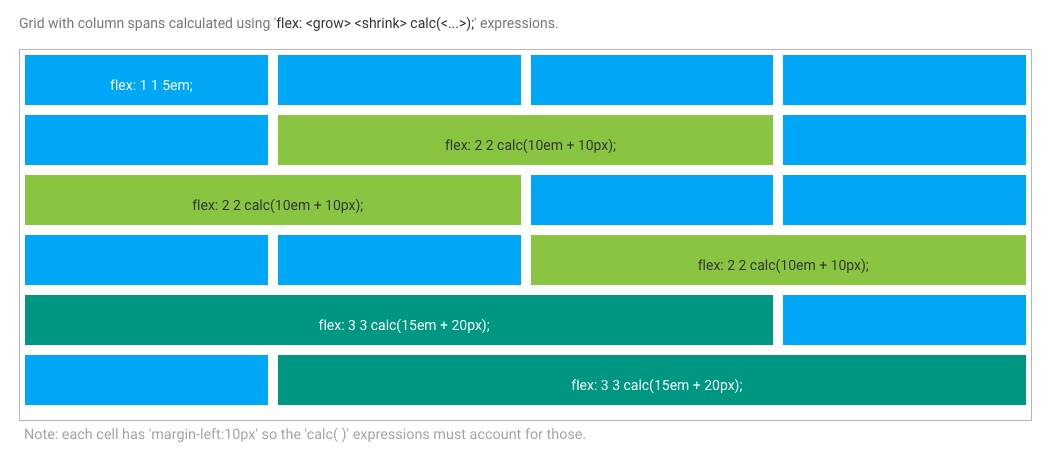
\includegraphics[width=12.1cm, height=9cm]{pwa/responsive/flex-layout/flex-layout-grid}
The following is the code which produces the above:
\\
\\
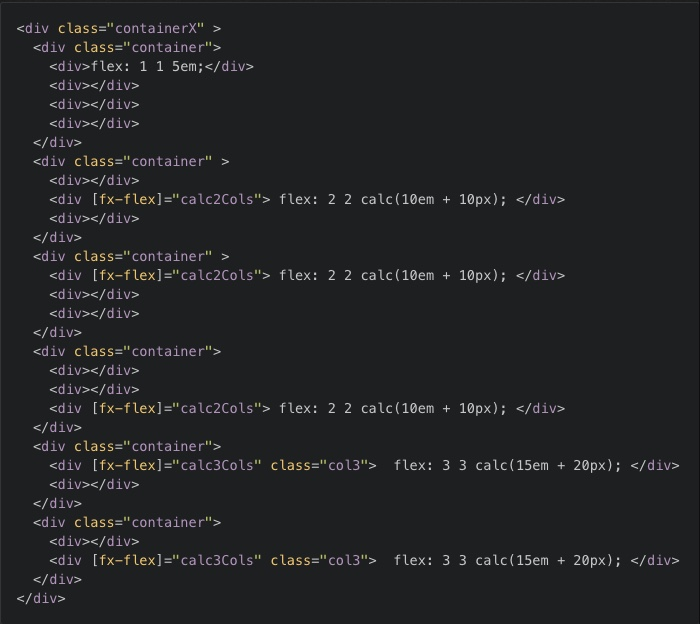
\includegraphics[width=12.1cm, height=9cm]{pwa/responsive/flex-layout/flex-layout-code}


\section{ Pixel Grid Container Layout }

Now that we have introduced Flex Layout and our designs call for three elements:
\begin{enumerate}
  \item Code Viewer
  \item Pixel Grid
  \item Color Picker
\end{enumerate}

\subsection{ Anticipate for Future Components }

We know that we will have three components that will be set up side by side.
On our main page component, which will contain all three, we will set the
following three fxLayout directives:
\begin{verbatim}
  fxLayout="row"
  fxLayout.xs="column"
  fxFlexFill
\end{verbatim}

The above is pretty straight forward. On screens not extra small, the layout
will be flex row. When the screen is extra small, the layout will be column.
With regards to fxFlexFill, it will populate the host element with the following:


\begin{tabular}{@{} l *4c @{}}
\toprule
 \multicolumn{1}{c}{Key} & Value \\
\midrule
 margin & 0         \\
 width  & 100\%     \\
 height & 100\%     \\
 min-width & 100\%  \\
 min-height & 100\% \\
\end{tabular}
\footnote{Taken from documentation here:
https://github.com/angular/flex-layout/wiki/fxFlexFill-API}

\subsection{ Adding FxLayout to Pixel Grid Page }

\subsubsection{ Add Flex Layout to App }
\begin{verbatim}
  npm i --save @angular/flex-layout
\end{verbatim}

\subsubsection{ Add Flex Layout to Pixel Grid Page Module }
\begin{lstlisting}
+import { FlexLayoutModule } from '@angular/flex-layout';

+    FlexLayoutModule,
\end{lstlisting}

\maketitle{}
\section{ Creating a Dumb Component }

\subsection {Outline}

\begin{enumerate}
  \item Create a UI dumb component in Lib folder
    \begin{enumerate}
      \item Use ClI to generate module
      \item Use ClI to generate component
    \end{enumerate}
  \item Import module into appropriate page
  \item Add component to page html
  \item Add proper styling to the illColorPicker
\end{enumerate}

\subsection {Create a UI Dumb Component in Lib Folder}
This is a dumb component, it should be created in the UI folder.
\footnote{Please reference the chapter discussing UI architecture for why
that is.}

\begin{lstlisting}
ng g lib color-picker --routing --directory="ui"
ng g component color-picker -a=color-picker --export
\end{lstlisting}

\subsection{ Add Color Picker to Pixel Grid Page Component }
Let's import our ill color picker into our Pixel Grid page.

\begin{lstlisting}
// pixel-grid-page.module.ts
+ import { IllColorPickerModule } from "@ill/ill-color-picker";
// in imports array
+ IllColorPickerModule
\end{lstlisting}

In addition, let's add the ill-color-picker component to our html.
\begin{lstlisting}
+ <ill-color-picker></ill-color-picker>
\end{lstlisting}

\subsection{ Add Styling Element to Create Basic  }
Let's add a basic width and height for out element.
\begin{lstlisting}
.IllColorPicker {
  display: flex;
  flex-direction: column;
  width: 200px;
  height: 100%;
}
\end{lstlisting}

\maketitle{}
\section{ Setting up Schematics Using Angular CLI }

In any project, one is ineviatbley going to have their architecture. It would
be extremely beneficial for one to create their own schematics. Primarily so,
that with a singular command line input, one would be able to generate all of
the files they need.

Schematics can be used to easily introduce and enforce project wide conventions.
This will easily ramp up time for new developers, as well as diminish time
spent on project for current developers.

\subsection{ Download Schematics Globally }
\begin{lstlisting}
  npm install -g @angular-devkit/schematics-cli
\end{lstlisting}

\subsection{ Create a file-directory Schematics }
While the application we are building specifically for this book is a pixel
illustrator, in practice the conventions we set up for this app, will be used
across the app. In a previous chapter we mentioned we mentioned the following
folder/file structure:
\\
\\
\begin{forest}
  [libs
    [common
      [animations
      ]
      [assets
      ]
      [core
       [auth]
       [guards]
       [pipes]
       [validators]
      ]
      [models
      ]
      [testing
      ]
      [ui
      ]
      [utils
      ]
      [styles
      ]
      [vendor
      ]
    ]
  ]
\end{forest}

If we do not enforce this using schematics, it can very difficult for other
teams to follow this folder structure. In addition, it will take quite a bit of
time to solve at high level.


\begin{lstlisting}
  schematics blank --name=px-schematics
\end{lstlisting}

\subsection{ Understanding Rules and Trees }
A Tree is a data structure that contains a base \footnote{A set of files that already exists}
and a staging area \footnote{A list of changes to be applied to the base}.

A Rule is a function that takes a Tree and returns another Tree. A RuleFactory
are functions that create a Rule.

The blank RuleFactory that we have so far:

\begin{lstlisting}
  import { Rule, SchematicContext, Tree } from '@angular-devkit/schematics';

  // You don't have to export the function as default. You can also have more
  // than one rule factory per file.

  export function pxSchematics(options: any): Rule {
    return (tree: Tree, _context: SchematicContext) => {
      tree.create(options.name || 'hello', 'world');
      return tree;
    };
  }

\end{lstlisting}

\mybox{
The options argument is an object that can be seen as the input of the factory.
From the CLI, it is the command line arguments the user passed. From another
schematic, it’s the options that were passed in by that schematic.
}

\subsubsection{ Tree Deepdive}
There are four methods that directly create a change in a Tree:
\begin{enumerate}
  \item create
  \item delete
  \item rename
  \item overwrite
\end{enumerate}

Similar to how we used create as an example above, to create a file, we also
have the option to use the schematic to delete, rename, or overwrite a file.

\subsubsection{ Generating a Folder using Schematics }

\maketitle{}
\section{ Schematics Deep Dive }

In the previous chapter we have created a px-schematics schematics. The first
thing that we are going to want to modify is the collection.json file for
px-schematics. Let's add an alias for 'px', as well as create a description.

\subsection{ Creating an Alias and Description }
\begin{lstlisting}
  "px-schematics": {
    "description": "Schematic for generating app folder structure",
    "aliases": ["app"],
    "factory": "./px-schematics/index#pxSchematics"
  }
\end{lstlisting}

\subsection{ Using NPM Link for development }
Being that we do not have an npm module yet, there is a super easy way to hook
up our custom schematic, to the actual Angular Schematics. Go into the root
of your project. For instance, for me that would be:
\begin{verbatim}
/Users/charlie/angularPixelillustrator
\end{verbatim}

Ok, so let's run:
\begin{verbatim}
npm link px-schematics
\end{verbatim}

\subsubsection{ What NPM Link Actually Does? }
When we ran npm link px-schematics, it automatically targeted our px-schematics
folder, and
\begin{lstlisting}
  /Users/charlie/angularpixelillustrator/node_modules/px-schematics ->
  /Users/charlie/.npm-global/lib/node_modules/px-schematics ->
  /Users/charlie/angularpixelillustrator/libs/px-schematics
\end{lstlisting}

\subsection{ Creating a schema.json for px-schematics }
The schema.json works like a regular schema, telling the CLI(command line
interface) what options can be used. In order to add a schema that is specific
for a collection create a schema.json file in you collection root. E.g.:
\begin{verbatim}
cd libs/px-schematics/src/px-schematics; touch schema.json;
\end{verbatim}

\begin{lstlisting}
  {
    "$schema": "http://json-schema.org/schema",
    "id": "px-schematics",
    "title": "Add px-schematics support to a app directory",
    "type": "object",
    "properties": {
      "name": {
        "type": "string",
        "description": "Name of the folder to contain files",
        "$default": {
          "$source": "argv",
          "index": 0
        }
      }
    }
  }
\end{lstlisting}
If we look at our schema.json file, we will notice, that it contains a couple
of important points. One is that a type field, string in our instance. Second,
that it has the familiar description key/value. In addition, we have created
name as a default. Therefore if we were to pass our schema an option, without
giving it a flag \footnote{For instance: \mybox{px angularPixelillustrator}}
then it will execute it by default.

\subsection{ Change Folder Architecture }
We are going to want to brace for future collections. So let's create a
collections folder to put our schematics into.
\begin{verbatim}
mdkir collections; mv px-schematics collections
\end{verbatim}

We are also going to modify our collections.json config to let schematics know
that we have our own schematics file. Our collections.json for px-schematics
should look like the following:

\begin{lstlisting}
{
  "$schema": "../node_modules/@angular-devkit/schematics/collection-schema.json",
  "schematics": {
    "px-schematics": {
      "description": "Schematic for generating app folder structure",
      "aliases": ["px"],
      "schema": "./collections/px-schematics/schema.json",
      "factory": "./collections/px-schematics"
    }
  }
}
\end{lstlisting}

\maketitle{}
\section{px schematics}

Now that we have deep dived into creating a schematic. We have the particulars
with regards to our application. We would like to architect a folder structure
that might include some repeat files, such as our app logo.

\mybox{
\subsection{A Word to the Wise}
First off, there is a need to run npm run build within the repo, everytime
that you go ahead and create a schematic. Otherwise, it will not work as
expected.
}

\subsection{Create a Files Directory}
Within our px-schematics, let's create a files directory:
\\
\\
\begin{forest}
  [libs
    [common
      [animations
      ]
      [assets
      ]
      [core
       [auth]
       [guards]
       [pipes]
       [validators]
      ]
      [models
      ]
      [testing
      ]
      [ui
      ]
      [utils
      ]
      [styles
      ]
      [vendor
      ]
    ]
  ]
\end{forest}

Due to how Angular Schematics works, we can go ahead and create a folder
directory as is, and supplant it within our app. We are going to create the
following folder directory with placeholder files for our app.

\maketitle{}
\section{ Nrwl Schematics }

We have gone into a deep dive with regards to creating custom schematics.
However, being that we are working with Nrwl schematics, there is a slightly
easier way for us to set up custom schematics within our app. It does tighly
couple our schematics with nrwl schematics, and for that reason I didn't like
it at first. However, after thinking about it, re-factoring the schematics to
be custom schematics wouldn't be the worst thing to happen.

In the previous chapters we created a schematic called the px-schematics. All it
did was generate files. For this task, we decided to go ahead and create our own
custom angular schematics. However, let's say we wanted to create our own
custom schematics, that made use of one of schematics nrwl already has available
for us, then it would definitely make sense to use the Workspace Specific
Schematics.

\subsection{ Workspace Specific Schematics }
\subsubsection{Generate a workspace specific schematic}
\begin{verbatim}
ng g workspace-schematic data-access
\end{verbatim}

Go to /tools/schematics/data-access/index.ts, where we will add in our custom
code.

\subsubsection{ Adding in External Schematics}
\begin{lstlisting}
externalSchematic('@nrwl/schematics', 'lib', {
  name: name,
  directory: schema.directory,
  tags: schema.directory ? `state, ${schema.directory}` : 'state, aero',
}),
externalSchematic('@nrwl/schematics', 'ngrx', {
  name: name,
  module,
  directory: '+state',
  facade: true,
}),
externalSchematic('@schematics/angular', 'service', {
  name: name,
  path: 'data-access',
  sourceDir: normalize(sourceDir),
  directory: schema.directory,
  app: schema.name,
}),
externalSchematic('@schematics/angular', 'interface', {
  name: name,
  path: 'data-access',
  sourceDir: normalize(sourceDir),
  directory: schema.directory,
  app: schema.name,
}),
\end{lstlisting}

First we include lib, so that we can choose which directory our schematics
should go in. Next we include ngrx, so that state is automatically generated
when we create a data-access. As part of our data access, we would like to
create a service as well, that will act as our liason between our GraphQL
requests, and our actual app. In addition, we will be creating an interface
file that will be used across all parts of our app. \footnote{Feel free to refer
back to the chapter on interfaces.}

\subsubsection{ Adding GraphQL Files }
One of the wonderful things about the Angular ecosystem, that schematics,
follows, is the amount of cookie cutter code. Creating your own schematics at
first can be daunting, however, the more we deep dive, we will find that we have
learnt the bulk of scheamtics. That is file generation and templating.

\maketitle{}
\section{ Color Picker }

Let's go through the steps again, being that we are creating our second
component. Part of learning is not only discovery, but maintenance. As discussed
in the preface, whenever we have the chance to repeat steps we have discussed
once before, we will re-iterate them on a high level for memory sake.

\subsection{ Outline of what needs to be done }
\begin{enumerate}
  \item Create a UI dumb component for color picker in Lib folder
    \begin{enumerate}
      \item Should be generated in app folder in UI folder.
      \item Use ClI to generate module
      \item Use ClI to generate component
    \end{enumerate}
  \item Import module into pixel-grid page
  \item Add component to pixel-grid page html
  \item Add proper styling to the illColorPicker
\end{enumerate}

\subsection{ CLI - Creation of Module and Component with Routing }
First, let's create our component in the lib folder of our app.

\begin{lstlisting}
ng g lib color-picker --routing --directory="dealworks/ui"
ng g component color-picker -a=color-picker --export
\end{lstlisting}

\subsection{ Add Color Picker to Pixel Grid Page Component }
Let's import our ill color picker into our Pixel Grid page.

\begin{lstlisting}
// pixel-grid-page.module.ts
+ import { IllColorPickerModule } from ``@ill/ill-color-picker';
// in imports array
+ IllColorPickerModule
\end{lstlisting}

In addition, let's add the ill-color-picker component to our html.
\begin{lstlisting}
+ <ill-color-picker></ill-color-picker>
\end{lstlisting}

\subsection{ Add Styling Element to Create Basic  }
Let's add a basic width and height for out element.
\begin{lstlisting}
.IllColorPicker {
  display: flex;
  flex-direction: column;
  width: 200px;
  height: 100%;
}
\end{lstlisting}

\end{document}